% UCL Thesis LaTeX Template
%  (c) Ian Kirker, 2014
% 
% This is a template/skeleton for PhD/MPhil/MRes theses.
%
% It uses a rather split-up file structure because this tends to
%  work well for large, complex documents.
% We suggest using one file per chapter, but you may wish to use more
%  or fewer separate files than that.
% We've also separated out various bits of configuration into their
%  own files, to keep everything neat.
% Note that the \input command just streams in whatever file you give
%  it, while the \include command adds a page break, and does some
%  extra organisation to make compilation faster. Note that you can't
%  use \include inside an \include-d file.
% We suggest using \input for settings and configuration files that
%  you always want to use, and \include for each section of content.
% If you do that, it also means you can use the \includeonly statement
%  to only compile up the section you're currently interested in.
% You might also want to put figures into their own files to be \input.

% For more information on \input and \include, see:
%  http://tex.stackexchange.com/questions/246/when-should-i-use-input-vs-include


% Formatting rules for theses are here: 
%  http://www.ucl.ac.uk/current-students/research_degrees/thesis_formatting
% Binding and submitting guidelines are here:
%  http://www.ucl.ac.uk/current-students/research_degrees/thesis_binding_submission

% This package goes first and foremost, because it checks all 
%  your syntax for mistakes and some old-fashioned LaTeX commands.
% Note that normally you should load your documentclass before 
%  packages, because some packages change behaviour based on
%  your document settings.
% Also, for those confused by the RequirePackage here vs usepackage
%  elsewhere, usepackage cannot be used before the documentclass
%  command, while RequirePackage can. That's the only functional
%  difference.
\RequirePackage[l2tabu, orthodox]{nag}


% ------ Main document class specification ------
% The draft option here prevents images being inserted,
%  and adds chunky black bars to boxes that are exceeding 
%  the page width (to show that they are).
% The oneside option can optionally be replaced by twoside if
%  you intend to print double-sided. Note that this is
%  *specifically permitted* by the UCL thesis formatting
%  guidelines.
%
% Valid options in terms of type are:
%  phd
%  mres
%  mphil
%\documentclass[12pt,phd,draft,a4paper,twoside]{ucl_thesis}
\documentclass[12pt,phd,a4paper,twoside]{ucl_thesis}


% Package configuration:
%  LaTeX uses "packages" to add extra commands and features.
%  There are quite a few useful ones, so we've put them in a 
%   separate file.
% -------- Packages --------

% This package just gives you a quick way to dump in some sample text.
% You can remove it -- it's just here for the examples.
\usepackage{blindtext}

% This package means empty pages (pages with no text) won't get stuff
%  like chapter names at the top of the page. It's mostly cosmetic.
\usepackage{emptypage}

% The graphicx package adds the \includegraphics command,
%  which is your basic command for adding a picture.
\usepackage{graphicx}

% This command is provided by the graphicx package, and 
%  controls the default dpi resolution of images you use.
%  72 is the default, but 300 is more normal, and 600 is
%  as good as you can expect to be able to get on normal paper.
\pdfimageresolution=300


% The float package improves LaTeX's handling of floats,
%  and also adds the option to *force* LaTeX to put the float
%  HERE, with the [H] option to the float environment.
\usepackage{float}

% The amsmath package enhances the various ways of including
%  maths, including adding the align environment for aligned
%  equations.
\usepackage{amsmath}

\usepackage{bm} % for \bm bold math command for matrices.

% Use these two packages together -- they define symbols
%  for e.g. units that you can use in both text and math mode.
\usepackage{gensymb}
\usepackage{textcomp}
% You may also want the units package for making little
%  fractions for unit specifications.
%\usepackage{units}


% The setspace package lets you use 1.5-sized or double line spacing.
\usepackage{setspace}
\setstretch{1.5}

% That just does body text -- if you want to expand *everything*,
%  including footnotes and tables, use this instead:
%\renewcommand{\baselinestretch}{1.5}


% PGFPlots is either a really clunky or really good way to add graphs
%  into your document, depending on your point of view.
% There's waaaaay too much information on using this to cover here,
%  so, you might want to start here:
%   http://pgfplots.sourceforge.net/
%  or here:
%   http://pgfplots.sourceforge.net/pgfplots.pdf
%\usepackage{pgfplots}
%\pgfplotsset{compat=1.3} % <- this fixed axis labels in the version I was using

% PGFPlotsTable can help you make tables a little more easily than
%  usual in LaTeX.
% If you're going to have to paste data in a lot, I'd suggest using it.
%  You might want to start with the manual, here:
%  http://pgfplots.sourceforge.net/pgfplotstable.pdf
%\usepackage{pgfplotstable}

% These settings are also recommended for using with pgfplotstable.
%\pgfplotstableset{
%	% these columns/<colname>/.style={<options>} things define a style
%	% which applies to <colname> only.
%	empty cells with={--}, % replace empty cells with '--'
%	every head row/.style={before row=\toprule,after row=\midrule},
%	every last row/.style={after row=\bottomrule}
%}


% The mhchem package provides chemistry formula typesetting commands
%  e.g. \ce{H2O}
%\usepackage[version=3]{mhchem}

% And the chemfig package gives a weird command for adding Lewis 
%  diagrams, for e.g. organic molecules
%\usepackage{chemfig}

% The linenumbers command from the lineno package adds line numbers
%  alongside your text that can be useful for discussing edits 
%  in drafts.
% Remove or comment out the command for proper versions.
%\usepackage[modulo]{lineno}
% \linenumbers 


% Alternatively, you can use the ifdraft package to let you add
%  commands that will only be used in draft versions
%\usepackage{ifdraft}

% For example, the following adds a watermark if the draft mode is on.
%\ifdraft{
%  \usepackage{draftwatermark}
%  \SetWatermarkText{\shortstack{\textsc{Draft Mode}\\ \strut \\ \strut \\ \strut}}
%  \SetWatermarkScale{0.5}
%  \SetWatermarkAngle{90}
%}


% The multirow package adds the option to make cells span 
%  rows in tables.
\usepackage{multirow}


% Subfig allows you to create figures within figures, to, for example,
%  make a single figure with 4 individually labeled and referenceable
%  sub-figures.
% It's quite fiddly to use, so check the documentation.
%\usepackage{subfig}

% The natbib package allows book-type citations commonly used in
%  longer works, and less commonly in science articles (IME).
% e.g. (Saucer et al., 1993) rather than [1]
% More details are here: http://merkel.zoneo.net/Latex/natbib.php
%\usepackage{natbib}

% The bibentry package (along with the \nobibliography* command)
%  allows putting full reference lines inline.
%  See: 
%   http://tex.stackexchange.com/questions/2905/how-can-i-list-references-from-bibtex-file-in-line-with-commentary
\usepackage{bibentry} 

% The isorot package allows you to put things sideways 
%  (or indeed, at any angle) on a page.
% This can be useful for wide graphs or other figures.
%\usepackage{isorot}

% The caption package adds more options for caption formatting.
% This set-up makes hanging labels, makes the caption text smaller
%  than the body text, and makes the label bold.
% Highly recommended.
\usepackage[format=hang,font=small,labelfont=bf]{caption}

% If you're getting into defining your own commands, you might want
%  to check out the etoolbox package -- it defines a few commands
%  that can make it easier to make commands robust.
\usepackage{etoolbox}





% This declares the unit "animals". Also redefined days to be whole word *(not sure if thats what is needed.
\usepackage{siunitx}
\DeclareSIUnit{\animals}{animals}
\DeclareSIUnit{\day}{day}




% Package to provide subfigures
\usepackage{subcaption}



% Package to provide comment environment
\usepackage{verbatim}

% This is included in KnitrSettings so that it is included in other tex documents.
% \usepackage{color}




% Sets up links within your document, for e.g. contents page entries
%  and references, and also PDF metadata.
% You should edit this!
%%
%% This file uses the hyperref package to make your thesis have metadata embedded in the PDF, 
%%  and also adds links to be able to click on references and contents page entries to go to 
%%  the pages.
%%

% Some hacks are necessary to make bibentry and hyperref play nicely.
% See: http://tex.stackexchange.com/questions/65348/clash-between-bibentry-and-hyperref-with-bibstyle-elsart-harv
\usepackage{bibentry}
\makeatletter\let\saved@bibitem\@bibitem\makeatother
\makeatletter\let\@bibitem\saved@bibitem\makeatother
\makeatletter

\makeatother
    


% And then some settings in separate files.
% These settings are from:
%  http://mintaka.sdsu.edu/GF/bibliog/latex/floats.html

% They give LaTeX more options on where to put your figures, and may
%  mean that fewer of your figures end up at the tops of pages far
%  away from the thing they're related to.

% Alters some LaTeX defaults for better treatment of figures:
% See p.105 of "TeX Unbound" for suggested values.
% See pp. 199-200 of Lamport's "LaTeX" book for details.

%   General parameters, for ALL pages:
\renewcommand{\topfraction}{0.9}	% max fraction of floats at top
\renewcommand{\bottomfraction}{0.8}	% max fraction of floats at bottom

%   Parameters for TEXT pages (not float pages):
\setcounter{topnumber}{2}
\setcounter{bottomnumber}{2}
\setcounter{totalnumber}{4}     % 2 may work better
\setcounter{dbltopnumber}{2}    % for 2-column pages
\renewcommand{\dbltopfraction}{0.9}	% fit big float above 2-col. text
\renewcommand{\textfraction}{0.07}	% allow minimal text w. figs

%   Parameters for FLOAT pages (not text pages):
\renewcommand{\floatpagefraction}{0.7}	% require fuller float pages
% N.B.: floatpagefraction MUST be less than topfraction !!
\renewcommand{\dblfloatpagefraction}{0.7}	% require fuller float pages

% remember to use [htp] or [htpb] for placement,
% e.g. 
%  \begin{figure}[htp]
%   ...
%  \end{figure} % For things like figures and tables


\addbibresource{epilit.bib}

   % For bibliographies

% Title Settings
\setcounter{secnumdepth}{3}
\setcounter{tocdepth}{3}
\title{The role of social ecology in Chiropteran pathogen richness and zoonotic potential}
\author{Tim C. D. Lucas}
\department{Centre for Mathematics and Physics in the Life Sciences and Experimental Biology }


\begin{document}



\nobibliography*
% This is a dumb trick that works with the bibentry package to let
%  you put bibliography entries whereever you like.
% I used this to put references to papers a chapter's work was 
%  published in at the end of that chapter.
% For more information, see: http://stefaanlippens.net/bibentry

% If you haven't finished making your full BibTex file yet, you
%  might find this useful -- it'll just replace all your
%  citations with little superscript notes.
% Uncomment to use.
%\renewcommand{\cite}[1]{\emph{\textsuperscript{[#1]}}}

% At last, content! Remember filenames are case-sensitive and 
%  *must not* include spaces.
\maketitle
%\makedeclaration

\begin{abstract} % 300 word limit

\lettr{P}athogens make up a huge proportion of global diversity and their role in disease strongly affects human disease, economics and development as well as having an important ecological role.
However, the factors that control the number of pathogen species are poorly understood.
In this thesis I examine the role population structure and density in maintaining these high levels of diversity in the face of interpathogen competition.
Throughout the thesis I focus on bats as a case study for more general disease processes as they have highly varied social structures and have emerged as important reservoires for zoonotic viruses such as Ebola, SARS, Hendra and Nipah.

In Chapter \ref{ch:empirical}





\end{abstract}

\begin{acknowledgements}
Acknowledge all the things!
\end{acknowledgements}

\setcounter{tocdepth}{2} 
% Setting this higher means you get contents entries for
%  more minor section headers.

\tableofcontents
\listoffigures
\listoftables




\chapter{Introductory Material}
\label{chapterlabel1}

\section{Pathogen richness and the impacts of zoonotic diseases}

\tmpsection{General intro}


\tmpsection{This diversity poses a zoonotic risk} %significance

Over 60\% of newly emerged diseases are zoonotic (acquired from animals) with wild animals being the predominant source \cite{jones2008global, woolhouse2006host, taylor2001risk}.
Zoonotic diseases can be extremely virulent with viruses such as Nipah  and Ebola having case fatality rates over 50\% \cite{luby2009recurrent, lefebvre2014case}.
Furthermore these pathogens can have large economic costs.
For example, SARS is estimated to have cost \$40 billion \cite{knobler2004learning}.
In particular these impacts can have huge effects on lower-income economies.
For example, both Liberia and Guinea experienced negative per capita growth rates of -2\% due to the Ebola epidemic in 2014 \cite{ebolaWorldbank, ebola2015worldbank}.
More generally, death rates per 1,000 people living with AIDS are up to ten times higher in developing countries than in Europe and North America \cite{granich2015trends}.
The global richness of pathogens is large but mostly unknown \cite{poulin2014parasite}.
Recent studies suggest that the global number of mammalian virus species is of the order of hundreds of thousands \cite{anthony2013strategy} while only 3,000 virus species, across all taxonomic groups, are currently described \cite{ICTV}.
This large pool of unknown pathogens presents a continuing risk of new pathogens spilling over into humans.


\tmpsection{Pathogen diversity has an important role in zoonotic diseases and we can optimise surveillance if we understand it}

Surveillance of zoonotic diseases is crucial for reducing the health impacts of these diseases.
In particular it is important to categorise and describe diseases before they spill over into humans.
For example, SARS was not identified until months into the pandemic \cite{drosten2003identification}. 
It is also important to improve our ability to predict when outbreaks will occur. 
For example, if it is known that there is \textit{i})~a higher disease prevalence in a given host species than normal, or \textit{ii})~a greater-than-usual abundance of a species that is a known reservoir of a high risk zoonotic disease, or \textit{iii})~increased contacts between humans and a pathogen reservoir, preparations can be made for a potential outbreak in that area.

However, funds for zoonotic disease surveillance are limited and so efforts must be optimised.
Knowing which species are likely to have many pathogens allows us to sample and identify potentially zoonotic viruses efficiently.
Suggested factors that might control pathogen richness include individual, environmental and population level traits.
Individual traits that have been studied include body mass and longevity.
Increased body mass is expected to increase pathogen richness as large bodies provide more resource for pathogens to consume and potentially more niches for them to occupy \cite{kamiya2014determines, arneberg2002host, poulin1995phylogeny, gomez2015diversity, bordes2008bat}.
Increased longevity is also expected to increase pathogen richness by increasing the number of pathogens a host encounters in its lifetime \cite{nunn2003comparative, ezenwa2006host, luis2013comparison}. 
Environmental factors may also play a role. 
Latitude has been studied as a proxy for environmental factors \cite{poulin2010latitudinal, kamiya2014determines}.
It is predicted that warmer climates promote species richness via metabolic mechanisms or by increasing the rate of evolution \cite{brown2004toward, dunn2010global, rohde1992latitudinal}.
Furthermore, population level traits that affect the dynamics of disease spread have also been studied.
Animal density \cite{kamiya2014determines, nunn2003comparative, arneberg2002host}, sociality \cite{bordes2007rodent, vitone2004body, altizer2003social, ezenwa2006host} and population structure \cite{nunes2006localized, maganga2014bat, gay2014parasite, turmelle2009correlates} have all been predicted to increase pathogen richness by increasing the rate of spread of new pathogens.
Finally, species with larger range sizes are expected to have higher pathogen richness as they experience a wider range of environments and have more sympatric host species \cite{kamiya2014determines, nunn2003comparative}.
These relationships can provide a basis for predicting which species will have high pathogen richness and should be prioritised for sampling and surveillance.

However, without a better mechanistic understanding of how pathogen richness is created and maintained it is difficult to predict how pathogen richness, and therefore zoonotic disease risk, will respond to global change.
Competition between pathogens can occur by different mechanisms: immunological mechanisms such as cross-immunity or shared immune response \cite{fenton2010applying} and ecological mechanisms such as removal of susceptible hosts by death \cite{rohani2003ecological} or competition for internal host resources \cite{griffiths2014analysis}.
As in ecological systems, competition leads us to the expectation that competitive exclusion occurs \cite{bremermann1989competitive, martcheva2013competitive, ackleh2003competitive, ackleh2014robust, turner2002impact}.
Therefore, the large number of coexisting parasite species needs an explanation.



\section{Influence of population size and structure on pathogen richness}


\tmpsection{Theoretical evidence that structure and density increase richness}

\subsection{Single-pathogen models}
% Structure + single path theory

In an unstructured, or well-mixed, population, epidemiological interactions --- events in which pathogens can potentially be transmitted --- occur randomly between individuals; an individual is equally likely to interact with any other individual.
In contrast, in a structured population, epidemiological interactions are not random.
This non-randomness can arise for many different reasons.
For example, the geographic distribution of individuals or social groups can both cause individuals to be more likely to interact with certain individuals than others.
Furthermore, different processes can structure a population depending on how pathogens are transmitted.
In the case of a sexually transmitted disease, epidemiological interactions only occur between mating individuals and the mating systems of the species will govern which individuals interact.
In contrast, if a pathogen is transmitted through the environment, by persisting in a water source for example, epidemiological interactions can occur between individuals that are never in close proximity to each other.
In these different cases, the processes by which population structure forms are different. %todo refs.

There is a large literature on the role of population structure on single-disease dynamics, as reviewed by \textcite{pastor2015epidemic}, driven by applications to human health as well as computer viruses \cite{pastor2001epidemic} and the social spread of information \cite{goffman1964generalization}.
In particular, work has concentrated on how population structure affects the basic reproduction number, $R_0$ \cite{colizza2007invasion, barthelemy2010fluctuation, wu2013threshold, may2001infection, pastor2001epidemic}.
Formally, $R_0$ is the average number of individuals infected by a single infected individual entering a na\"ive population where no individuals have previously acquired immunity to the pathogen of interest.
More intuitively, $R_0$ combines relevant parameters to yield a threshold above which a disease is expected to infect a significant proportion of the population \cite{may1979population, anderson1979population}.
Below the threshold, only small outbreaks that quickly die out are expected.
% Density + single path theory

The roles of population size and density in the dynamics of single pathogens are also well established \cite{may1979population, anderson1979population, heesterbeek2002brief, lloyd2005should}.
Broadly, larger populations can maintain a disease more easily by having a larger pool of susceptible individuals (individuals without acquired immunity) and having a greater number of new susceptible individuals enter the population by birth or immigration \cite{may1979population, anderson1979population}.
High density populations are expected to have a greater number of contacts between individuals and so promote the spread of a pathogen.
However, there is much discussion about if, and when, the number of contacts might scale independently of density \cite{mccallum2001should}.

\subsection{Multi-pathogen models}
% multi path is important
While the majority of theoretical work considers single pathogens, with models examining whether a pathogen can spread and persist in a population, much less work has been done on multiple pathogen systems.
Studies have found tens \cite{anthony2013strategy} or even hundreds \cite{anthony2015non} of virus species in a single host species.
%This suggests that the global number of mammalian virus species is of the order of hundreds of thousands \cite{anthony2013strategy} while recent large databases include nearly 2,000 pathogens from approximately 400 wild animal hosts \cite{wardeh2015database}.
Therefore ignoring inter-pathogen competition is an oversimplification.

% structure and multi theory
A number of studies have considered the case where two pathogens spread concurrently and examine which pathogen infects more individuals.
These studies have found that increased population structure reduces dominance of the more competitive strain \cite{van2014domination, poletto2013host, poletto2015characterising}.
However, this again reveals little about how pathogen communities form and what factors control total pathogen richness.
Far fewer papers explicitly study long term coexistence of two or more pathogens.
Those that do commonly find that competitive exclusion is likely \cite{castillo1995dynamics, bremermann1989competitive, martcheva2013competitive, ackleh2003competitive, ackleh2014robust, turner2002impact}.
Mechanisms that have been shown to allow pathogen coexistence include superinfection \cite{may1994superinfection, li2010age}, density-dependent deaths \cite{ackleh2003competitive, kirupaharan2004coexistence} and differing transmission routes \cite{allen2003dynamics}.

% density + multi theory
The specific role of density on the ability of pathogens to coexist has not been theoretically studied though it is commonly found to promote pathogen richness in comparative empirical studies \cite{kamiya2014determines, nunn2003comparative, arneberg2002host}.
The few papers that have directly studied how coexistence of pathogens responds to population structure have found that population structure can allow pathogens to coexist even though competitive exclusion would occur in a fully mixed population \cite{qiu2013vector, allen2004sis, nunes2006localized}.
Furthermore, genetic diversity has been shown to be maximised at intermediate levels of population structure \cite{campos2006pathogen}.
The roles of population structure and social group size have been examined in comparative studies \cite{maganga2014bat, gay2014parasite, turmelle2009correlates, altizer2003social, bordes2007rodent, ezenwa2006host, rifkin2012animals, vitone2004body}.
There is much disagreement between these studies.
Population structure has been shown to promote \cite{maganga2014bat, turmelle2009correlates} and inhibit pathogen richness \cite{gay2014parasite}.
Similarly, group size has been shown to promote \cite{rifkin2012animals, bordes2007rodent} and inhibit \cite{ezenwa2006host} pathogen richness.
While increased group size should generally decrease population structure, the literature is rarely clear on the relationships between these and other variables.



\tmpsection{Specific intro}

\section{Bats as reservoirs of zoonotic diseases}

\tmpsection{Bats are a particular culprit of this risk, and have unknown diversity and interesting population structure.} %context

In recent decades bats have been implicated in a number of high profile zoonotic outbreaks such as Nipah \cite{field2001natural, halpin2011pteropid}, Ebola \cite{leroy2005fruit}, SARS \cite{li2005bats} and Hendra \cite{field2001natural}.
These outbreaks have led to much research on whether bats are a particularly important source of zoonotic disease \cite{luis2013comparison, olival2015bats, wang2011mass} and examinations of factors, such as flight, social living and longevity, that might predispose them to being reservoirs of zoonotic viruses \cite{calisher2006bats, o2014bat, dobson2005links, racey2015uniqueness, kuzmin2011bats}.
Given that bats are the second largest order of mammals \cite{wilson2005mammal}, we may expect them to be the source of many viruses simply through weight of numbers \cite{luis2013comparison}.
The broad conclusions are that while bats do host more zoonotic virus species than other groups \cite{luis2013comparison} they do not host more virus species per host species \cite{olival2015bats}.


Many factors of bat populations make them epidemiologically interesting.
They have highly varied and sometimes complex social structures \cite{kerth2008causes}.
Some species are largely solitary or live in very small groups --- e.g., \emph{Lasiurus borealis} \cite{shump1982lasiurus} --- while other species live in colonies of millions of individuals --- e.g., \emph{Pteropus scapulatus} \cite{birt2008little}.
These groups can be very stable \cite{kerth2011bats, mccracken1981social}.
Further complexity arises due to their propensity for seasonal migration \cite{fleming2003ecology, richter2008first, cryan2014continental} and seasonally changing social organisation such as maternity roosts, hibernation roosts and swarming sites \cite{kerth2008causes}.
Finally, their ability to fly means that populations can be well mixed across large distances \cite{peel2013continent, petit1999male}, though this is highly variable with some species having limited dispersal \cite{wilmer1994extreme}.

However, the population density of many bat species, particularly tree roosting species, is unknown \cite{clement2013estimating}.
As they are small, nocturnal and difficult to identify in flight, estimating their density is incredibly difficult without disruptive and time-consuming roost surveys \cite{kloepper2016estimating, humphrey1971photographic, sabol1995technique}.
Furthermore, bat densities are generally estimated by counting bats in roosts and dividing this number by area which assumes all roosts have been surveyed \cite{speakman1991minimum, zahn2006population, moreno2004colony}. 
As density is associated with pathogen richness \cite{kamiya2014determines} and central to epidemiological models \cite{may1979population, anderson1979population} this leaves large gaps in our understanding of disease processes in this taxon.

\tmpsection{Bats are hard to detect etc.}




\section{Thesis overview}

In this thesis I examined the role of population structure and density on pathogen richness.
I used bats as a case study throughout due to their interesting social structure and importance as zoonotic	reservoirs.
I combined empirical, comparative studies with simulation models.
This allowed me to study specific mechanisms while linking my theoretical insights to real-world, empirical tests of hypotheses.


\tmpsection{Chapter 2}

First, in Chapter~\ref{ch:empirical}, I empirically tested the hypothesis that population structure is associated with pathogen richness (measured as known viral richness) in wild bat populations.
To ensure robust results I used two measures of population structure --- the number of subspecies and gene flow --- and a larger data set than previous studies.
For both measures I found that bat species with more structured populations have more known viruses.
This relationship is still present after controlling for study bias and phylogenetic nonindependence.
I also tested for relationships between body mass and pathogen richness, and range size and pathogen richness, and found strong support for larger bodied bats carrying more viruses and mixed support for range size promoting pathogen richness.

\tmpsection{Chapter 3}

In Chapter~\ref{ch:sims1}, I examined one specific mechanism by which population structure may promote increased pathogen richness.
I tested whether increased population structure can allow newly evolved pathogen strains to invade and persist more easily.
I modelled bat populations as individual-based, stochastic metapopulations and examined the competition dynamics of two identical pathogen strains.
I tested two factors related to host population structure: dispersal rate and the number of links between colonies.
I found that increased dispersal rate significantly increased the probability of a newly evolved pathogen invading and persisting in the population.
However, this was only the case at intermediate transmission rates.
I did not find a significant difference in invasion probability due to the number of links between colonies.

\tmpsection{Chapter 4}

Next, I examined the relationships between a number of elements of population structure (Chapter~\ref{ch:sims2}).
I clarified the interdependence between range size, population size and density.
I also noted that population size can be decomposed into colony size and the number of colonies.
Using the same model as in Chapter~\ref{ch:sims1}, I then tested which of these factors are most important in promoting pathogen richness.
Specifically I tested which factor most strongly promotes the invasion and establishment of newly evolved pathogens.
I found that population size is more important than population density and that colony size is the important component of population size.

\tmpsection{Chapter 5}

Given the importance of host population size and density on pathogen richness it is important to have good population estimates for wild bat populations.
However, there are currently very few measurements of bat population size due to their small size, nocturnal habit and difficulties in identification.
Therefore I aimed to develop a method for estimating bat population size from acoustic data, specifically data collected by the iBats project \cite{jones2011indicator}.
In Chapter~\ref{ch:grem} I developed a generally applicable method --- based on random encounter models \cite{rowcliffe2008estimating, yapp1956theory} --- for estimating population sizes of animal populations using camera traps or acoustic detectors.
I used spatial simulations to test the method for biases and to assess its precision.
I found that the method is unbiased and precise as long as a reasonable amount of data is collected.


\tmpsection{Chapter 6: Conclusions}

%to do Conclusions chapter
Finally, in Chapter~\ref{ch:discussion}, I discuss broader conclusions, applications and implications of my results.
I also discuss potential future directions for research.














\chapter{Does network structure of bat populations promote viral diversity?}
\label{chapterlabel2}

\clearpage
\section{Abstract}

\subsubsection{One or two sentences providing a basic introduction to the field}
% comprehensible to a scientist in any discipline.
An increasingly large fraction of emerging diseases come from animals and these diseases have a huge impact on human health.
The chance that a new disease will come from any particularly wild host species increases with the diversity of pathogens in that species.
However, the factors that control pathogen diversity in wild populations are still unknown.



\subsubsection{Two to three sentences of more detailed background}
% comprehensible to scientists in related disciplines.

% Add mechanistic vs empirical
Host species traits such as population density, longevity, body size and population structure have been shown to correlate with pathogen diversity.
However, our mechanistic understanding of how population structure (i.e. non random contacts across the population creating barriers to disease spread) affects pathogen diversity is poor.
Greater mechanistic understanding is needed to clarify the exact causal role population structure has in controlling pathogen diversity.
Mechanistic models are also likely to be more robust to transfering understanding between taxa and predicting changes. % !!! Not great.

Typically it is assumed that well-connected populations promote disease spread (high $R_0$) and therefore promote pathogen diversity.
However, if competition is strong endemic pathogens will dominate and prevent new diseases from invading and spreading.
In a structured population, stochastic effects could create areas of low prevalence of the endemic disease, allowing new diseases to invade.

We consider bats as a case study as they have been implicated in a number of recent, high profile diseases such as Ebola, SARS, Hendra and Nipah.
Bats have varied social structures and so the structure of populations could be one way to prioritize zoonotic disease surveillance in this group.

\subsubsection{One sentence clearly stating the general problem (the gap)}
% being addressed by this particular study.
It is unknown whether population structure allows escape from competition and therefore high diversity.

We hypothesise that low dispersal rates and a low number of connections in a metapopulation network will allow invading pathogens to establish more readily. 

\subsubsection{One sentence summarizing the main result}
%  (with the words “here we show” or their equivalent).
I find that neither population connectedness nor dispersal rate affect the probability that a new pathogen will invade into a population.

\subsubsection{Two or three sentences explaining what the main result reveals in direct comparison to what was thought to be the case previously}
% or how the main result adds to previous knowledge
The common assumption that factors causing high $R_0$ allow new pathogens to invade and therefore increase pathogen diversity is not supported by our study.
Instead we find that changes in population structure that would affect $R_0$ do not affect the probability of invasion of a new pathogen.


\subsubsection{One or two sentences to put the results into a more general context.}
This result means that large scale population structure does not seem to control pathogen diversity.
This also implies that population structure is not a useful proxy for pathogen diversity with respect to zoonotic disease surveillance, for example in bats.


\subsubsection{Two or three sentences to provide a broader perspective, }
% readily comprehensible to a scientist in any discipline.





%%%%%%%%%%%%%%%%%%%%%%%%%%%%%%%%%%%%%%%%%%%%%%%%%%%%%%%%%%%%%%%%%%%%%%%%%%%%%%%%%%%%%%%%%%%%%%%%%%%%%%%%%%%%%%%%%%%%%%%%%%%%%%%%%%%%%%%%%%%%%%%%%%%%%%%%%%%

\clearpage
\section{Introduction}

%%%%%%%%%%%%%%%%%%%%%%%%%%%%%%%%%%%%%%%%%%%%%%%%%%%%%%%%%%%%%%%%%%%%%%%%%%%%%%%%%%%%%%%%%%%%%%%%%%%%%%%%%%%%%%%%%%%%%%%%%%%%%%%%%%%%%%%%%%%%%%%%%%%%%%%%%%%




\subsection{General Intro}
%%%%%%%%%%%%%%%%%%%%%%%%%%%%%%
% A basic introduction to the field,
% comprehensible to a scientist in any discipline.


\subsubsection{Why is pathogen diversity important?}

The diversity of pathogens in a wild animal species strongly affects the chance that a disease from that species will infect humans.
As over 50\% of emerging infectious diseases have an animal source  \cite{jones2008global}, understanding and predicting this process is a global health priority.
However, the factors that control the diversity of pathogens in a wild animal population are still unclear.


\subsubsection{We know some factors that correlate with pathogen diversity}
A number of host traits have been shown to correlate with pathogen richness including body size  \cite{}, longevity  \cite{} and social structure  \cite{}.
However, studies are often contradictory due to small sample sizes, noisey data and because empirical relationships often do not generalise across taxa.
Furthermore, the correlation between many traits makes it hard to clearly distnguish which factors are important.
Knowing the factors that correlate with pathogen richness also does not tell us how it controls richness. 
Mechanisms by which a trait could increase pathogen diversity include promoting the evolution of new strains within a species, reduction of the rate of parasite extinction and an increased probability of pathogen invasion.



\subsubsection{But we do not understand the mechanistic processes}

We largely do not understand the mechanisms behind how these traits control pathogen diversity.




\subsubsection{We cannot assume high $R_0$ gives high diversity}
The processes by which a disease spreads through a population are very well studied.
One commonly taken assumption is that factors that promote high disease spread automatically promotes high diversity.
However, this ignores competitive mechanisms such as cross-immunity and depletion of susceptible hosts.
If competitive mechanisms are strong, then pathogens in populations structured such that $R_0$ will be high will be able to easily out-compete invading pathogens.
If competitive mechanisms are weak, then high $R_0$ will enable the invasion of new pathogens and allow higher pathogen diversity.




\subsection{Specific Intro}
%%%%%%%%%%%%%%%%%%%%%%%%%%%%%%
% more detailed background}
% comprehensible to scientists in related disciplines.


\subsubsection{Population structure could be important}
One host-species trait that has been largely understudied with respect to pathogen diversity is population structure.
Population structure has been comprehensively studied with respect to single or competing epidemics in human populations, wildlife populations and technological networks.
However, as explained above, the assumption that population structures that yield high $R_0$ will also give high pathogen diversity is unfounded.



\subsubsection{Network structure has been studied}
 
% Analytical models

Studies of the role of population structure on pathogen diversity have been in very simple systems.
These have been so simple that empirical data cannot easily be applied to them to predict pathogen diversity of real wild animal populations.
There is a need for models that can be carefully and fully explored, while still capturing the complexities of the real world.

Analytical models have different outcomes for well mixed populations: infinite diversity out competitive exclusion.
When competitive exclusion ours, population structure has sometimes been shown to allow coexistence.



Competing epidemics

  \cite{poletto2013host, poletto2015characterising, karrer2011competing}

Single pathogen epidemics






\subsubsection{Empirical evidence that structure might affect diversity}


Maganga \emph{et al.} found that distribution fragmentation predicts viral richness   \cite{maganga2014bat}, but   \cite{gay2014parasite} finds the opposite relationship. 
While the dataset in   \cite{gay2014parasite} is larger, the analysis in   \cite{maganga2014bat} is much more focused on fragmentation.

Genetic correlates of population structure have also been used.
Turmelle \emph{et al.}   \cite{turmelle2009correlates}, in a small analysis, find that high $F_{st}$ (i.e. a structured population) correlates with high richness.



\subsubsection{Types of population structure}

How structured a population is can be defined in many ways on many scales.
The most relevant scale is that of an epidemiological population.
This is the population within which a pathogen can spread in an epidemiologically relevant time period (years or decades).
It is therefore closely related to a population as defined by population genetics, but with movement defined on a shorter time scale.

The epidemiological contacts within the population can be examined at the individual level (as in contact network epidemiology) or larger scales.
We consider the metapopulation network the most appropriate.
Ignoring the metapopulation assumes a fully mixed population which is unlikely.
Trying to study the contact network relies detailed individual level detail which is not available.
Metapopulation models consider a network of small subpopulations. 
Within subpopulations, epidemiological contacts are fully mixed and relatively fast.
Between subpopulations, epidemiological contacts are dependant on an underlying network structure and relatively slow.
The network underlying the metapopulation is made up of nodes representing the subpopulations, and edges which represent movement between subpopulations.
Animals, and therefore infection, can only move between two subpopulations if they are connected by an edge.

There are two factors that affect how structured a population is, given this model framework.
Firstly, dispersal is the rate at which individuals move between subpopulations.
Secondly, the metapopulation network structure controls population structure.
The simplest measure of how structured the network is the average number of edges each node has.
In the extremes, all subpopulations could be either connected to all other subpopulations or only connected to one or two other subpopulations.
However, other measures that take into account second-order structure in the network are also often used.




\subsubsection{Why bats}
Bats (Order Chiroptera) have, over the last decade, become a focus for disease research  \cite{calisher2006bats, hughes2007emerging}.
Recently they have been implicated in a number of high profile diseases such as Ebola, SARS, Hendra and Nipah  \cite{calisher2006bats, li2005bats}.


\subsubsection{Describe bats}

Bats have an unusual variety of social structures.
Group living ranges from colonies 10--1 million \cite{jones2009pantheria}.



\subsection{The gap}
%%%%%%%%%%%%%%%%%%%%%%%%%%%%%%
% One sentence clearly stating the general problem
% being addressed by this particular study.
% By this stage, must have defined/introduced all terms used within.

We have very abstract, simplified models that predict zero or infinite diversity depending on specifics.
These cannot be easily applied to real data.
they also do not easily predict quantitative or even relative diversity as they often predict either zero or infinite diversity with nothing in between.

We need models that can quantitatively or at least relatively predict diversity in a populations.
This requires a middle ground of model diversity.

Furthermore there are few studies that aim to predict bat pathogen diversity.
There are no studies that directly model bat pathogen diversity.

Specifically we use these models to test the affects of population structure on the ability of a new pathogen to invade a population.
We test two aspects of structure, dispersal rate and connectedness of the metapopulation network.


\subsection{What I did}
%%%%%%%%%%%%%%%%%%%%%%%%%%%%%%


I have run epidemiological simulations based broadly on real world bat populations.
Although still simplified, the model is complex enough that if good measurements of bat populations could be found, simulations of the real world bat population could be run.




\subsection{What I found}
%%%%%%%%%%%%%%%%%%%%%%%%%%%%%%
% One sentence summarizing the main result
% (with the words “here we show” or their equivalent).


\begin{table}[t]
\begin{tabular}{>{\it}lp{8cm}l}
\normalfont{Term} & Definition & Synonyms \\
\hline
Metapopulation & A group of colonies with rare movement of animals between them. Closed to outside migration. & Network\\
Subpopulation & A group of animals. Social interactions within a colony is likely high. & Node, colony\\
Dispersal & Movement from one colony to another  & Migration\\
Population & A closed group of animals. No epidemiological affects from outside the group on epidemiological timescale (years -- decades.) & \\
Pathogen diversity & The number of species or strains of pathogens in a host & Pathogen richness\\
Connectedness &  & \\

\end{tabular}
\caption{Glossary of terms}
\label{t:glossary}
\end{table}


%%%%%%%%%%%%%%%%%%%%%%%%%%%%%%%%%%%%%%%%%%%%%%%%%%%%%%%%%%%%%%%%%%%%%%%%%%%%%%%%%%%%%%%%%%%%%%%%%%%%%%%%%%%%%%%%%%%%%%%%%%%%%%%%%%%%%%%%%%%%%%%%%%%%%%%%%%%

\clearpage
\section{Methods}

%%%%%%%%%%%%%%%%%%%%%%%%%%%%%%%%%%%%%%%%%%%%%%%%%%%%%%%%%%%%%%%%%%%%%%%%%%%%%%%%%%%%%%%%%%%%%%%%%%%%%%%%%%%%%%%%%%%%%%%%%%%%%%%%%%%%%%%%%%%%%%%%%%%%%%%%%%%


\subsection{Metapopulation model}





\subsubsection{Two pathogen SIR model}

We examine a multpathogen SIR model. 
This is a compartment model with individuals being classed as susceptible, infected or recovered with immunity (Figure~\ref{f:sir}).
Susceptible individuals are counted in class $S$.
There are three infected classes, $I_1$, $I_2$ and $I_{12}$, being individuals infected with pathogen 1, pathogen 2 or both respectively.
Recovered individuals, $R$, are immune to both pathogens, even if they have only been infected with one.
Furthermore, recovery from a pathogen moves an individual straight into the recovered class, even if the individual is infected with both pathogen.
This modelling choice allows the model to be easily expanded to included more than two pathogens.
The assumption of immediate recovery from all other diseases is likely to be quite accurate for very closely related pathogens as is being studied here as once an acquired immune response is activated, all infections are likely to be cleared quickly.
The coinfection rate is adjusted compared to the first infection rate by a factor $\alpha$.

Birth and death rates are assumed to be equal, $b = d$.


\begin{figure}[b]
\centering

  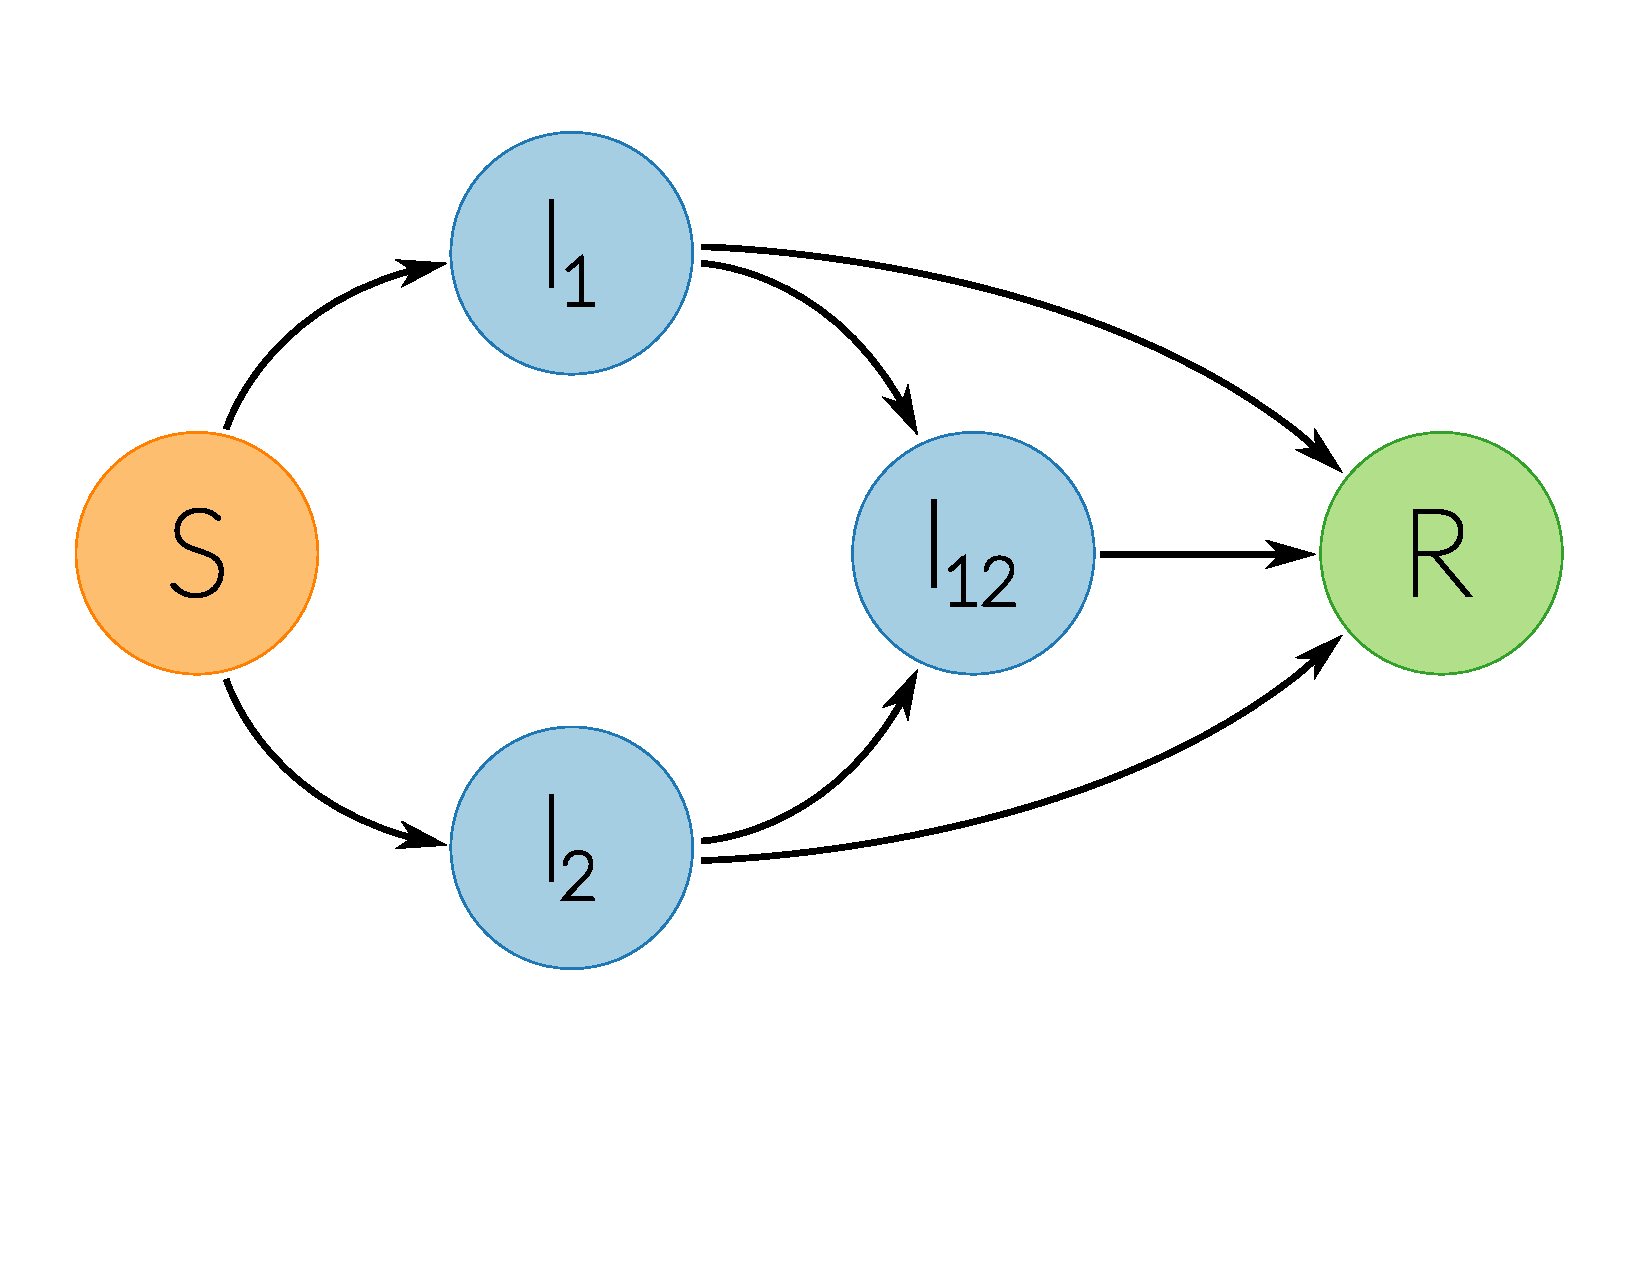
\includegraphics[width=0.4\textwidth]{imgs/SIRoption1.pdf}
  \caption{The SIR model used.}
  \label{f:sir}
\end{figure}

\subsubsection{Metapopulation}

The population is divided into a number of subpopulations.
This metapopulation is modelled as a network with subpopulations being nodes and dispersal between subpopulations being indicated by edges (Figure~\ref{f:net})
Individuals with a subpopulation interact randomly so that the subpopulation is fully mixed.
However, dispersal between subpopulations occurs at a rate $\lambda$.
Individuals can only disperse to subpopulations connected to theirs in the network.
The rate of dispersal is not affected by the number of edges a subpopulation has (the degree of the subpopulation).
So the dispersal rate from a subpopulation $m$ with degree $k_m$ to subpopulation $n$ is $\frac{\lambda}{k_m}$.
Note this rate is independant of the degree of subpopulation $n$.


\subsubsection{Stochastic simulations}

We examine this model using stochastic, continuous time simulations using the Gillespie algorithm.
At each step in the simulation we calculate the rate that each possible event might occur.
One event is then randomly chosen, weighted by it's rate
\begin{align}
  p(\text{event } i) = \frac{r_i}{\sum_i r_i}
\end{align}
where $r_i$ is the rate that event $i$ occurs.
Finally, the length of the time step, $\delta$, is drawn from an exponential distribution 
\begin{align}
  \delta \sim \operatorname{Exp}\left(\sum_i r_i  \right).
\end{align}
This means that the length of each simulation is stochastic. 
We define the number of events we wish to simulate instead.

We can now write down the rates of all events. I define $I^+_p$ to be the sum of all classes that are infectious with pathogen $p$, for example $I^+_1 = I_1 + I_{12}$. Assuming asexual reproduction, that all classes reproduce at the same rate and that individuals are born into the susceptible class we get
\begin{align}
P\left( S_{nt^\prime} = S_{nt} +1\right) &= b\left( S_{nt}+\sum_q I_{qnt} + R_{nt}\right) 
\end{align}
where $P\left( S_{nt^\prime} = S_{nt} +1\right)$ is the probability that the number of susceptibles in subpopulation $n$ will increase by 1 (a single birth) the short time interval $t$ to $t^\prime$ and $\sum_q I_{qnt}$ is the sum of all infection classes $q \in {1, 2, 12}$.
The rates of death, given a death rate $d$ are given by
\begin{align}
P\left( S_{nt^\prime} = S_{nt}-1 \right) &= dS_{nt} \\
P\left( I_{qnt^\prime} = I_{qnt}-1 \right) &= dI_{qnt}\\
P\left( R_{nt^\prime} = R_{nt}-1 \right) &= dR_{nt}.
\end{align}
Infection of a susceptible with either pathogen 1 or 2, $S \rightarrow I_p$ where $p\in \{1,2\}$, is given by
\begin{align}
P\left( I_{pnt^\prime} = I_{pnt}+1, S_{nt^\prime} = S_{nt}-1 \right) &= \beta S_{nt}I^+_{pnt},
\end{align}
while coinfection, given a crossimmunity factor $\alpha$, is given by
\begin{align}
P\left( I_{12,nt^\prime} = I_{12,nt}+1,\: I_{pnt^\prime} = I_{pnt}-1\right) = \alpha\beta I_{nt}I^+_{pnt}.
\end{align}
The probability of migration from colony $m$ (with degree $k_m$) to colony $n$, given a dispersal rate $\lambda$ is given by
\begin{align}
P\left(S_{nt^\prime}=S_{nt}+1,\: S_{mt^\prime} = S_{mt}-1\right) &= \frac{\lambda S_{mt}}{k_m-1}\\
P\left(I_{qnt^\prime}=I_{qnt}+1,\: I_{qmt^\prime} = I_{qmt}-1\right) &= \frac{\lambda I_{qmt}}{k_m}\\
P\left(R_{nt^\prime}=S_{nt}+1,\: R_{mt^\prime} = R_{mt}-1\right) &= \frac{\lambda R_{mt}}{k_m}.
\end{align}
Finally, recovery from any infectious class occurs at a rate $\gamma$
\begin{align}
P\left( I_{qnt^\prime} = I_{qnt}-1,\: R_{nt^\prime} = R_{nt}+1 \right) &= \gamma I_{qnt}.
\end{align}



In each simulation the population is seeded with 200 infected individuals of disease 1 in each colony. 
Disease 1 is then allowed to spread and reach equilibrium. 
After 40,000 events, 10 individuals infected with disease 2 are added to one colony. 
After another 10,000 events the invasion of disease 2 is considered successful if any individuals with the disease still remain.



\subsection{Parameter selection}

The values used for the independant variables are chosen to highlight the affects of these variables. 
The network structure is synthetically created to be either fully or minimally connected (i.e. a ring). 
10 subpopulations was selected as a trade off between computation time and a network complicated enough that structure might have an effect. 
This value is artificially small compared to wildlife populations. 

Dispersal values are $\lambda = 0.1, 0.01 and 0.001$ dispersals per year. 
$\lambda = 0.1$ relates to individuals moving between colonies on average twice per lifetime. 
Therefore exclusively juevinile dispersal would have dispersal rates similar to this. 
Otherwise it relates to dispersal being a rare event with animals often staying in a colony for many years.
$\lambda = 0.01$ relates to 20\% of individuals dispersing once in their lifetime.
This value is therefore close to male-biased dispersal, with female philopatry. 
Finally, $lambda = 0.001$ relates to 2\% of invididuals dispersing in their lifetime.
This therefore relates to a population that does not habitually disperse.



The fixed parameters used are chosen to roughly reflect realistic wild bat populations. 
The death rate $d$ is set as 0.05 per year giving a generation time of 20 years.
The birth rate $b$ is set to be equal to $d$ so that the population size is stable.
The recovery rate $\gamma$ is set to 0.1 giving a average infection duration of 10 years. 
This is therefore a chronic infection. 
It is very difficult to directly estimate infection durations in wild populations.
But it seems that these infections might be long lasting \cite{}.

Cross immunity is set to 0.1 so that an individual infected with one disease is 90\% less likely to be infected with another.
This is a rather arbitrary value.
However, the model assumes complete cross immunity after infection.
Furthermore, the rationale of some modelling choices is that the invading species might be a newly speciated strain of the endemic species.
Therefore cross immunity is likely to be very strong.





Three values of the transmission rate $\beta$ are used, 2, 5 and 10.


\subsection{Dispersal}
%%%%%%%%%%%%%%%%%%%%%%%%%%%%%%



\subsection{Network structure}
%%%%%%%%%%%%%%%%%%%%%%%%%%%%%%


\begin{figure}[b]
\centering
        \begin{subfigure}[b]{0.35\textwidth}
                \centering
		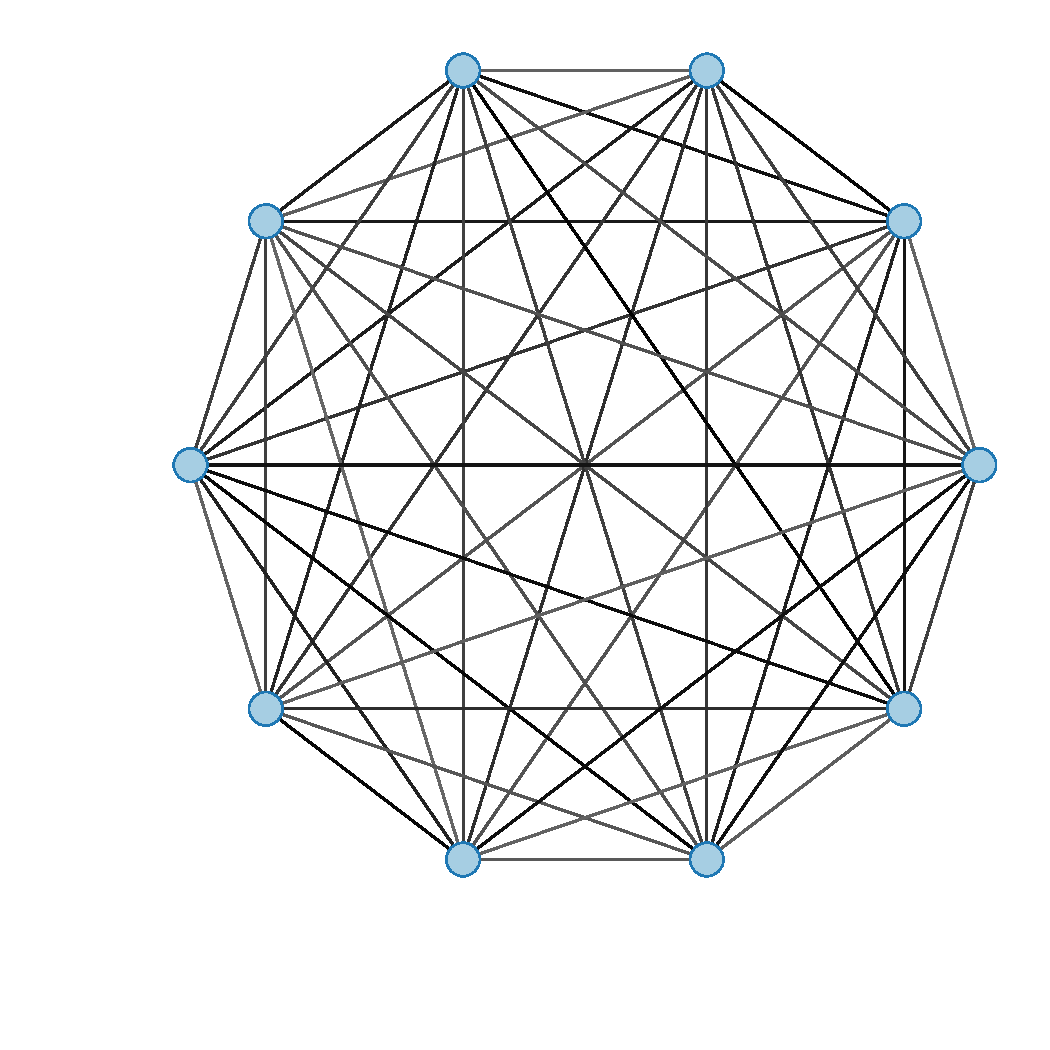
\includegraphics[width=1\textwidth]{imgs/fullyConnected.pdf}
                \caption{High $\bar{k}$}
                \label{fig:fullyConnected}
        \end{subfigure}
        ~ 
	\begin{subfigure}[b]{0.35\textwidth}
                \centering
		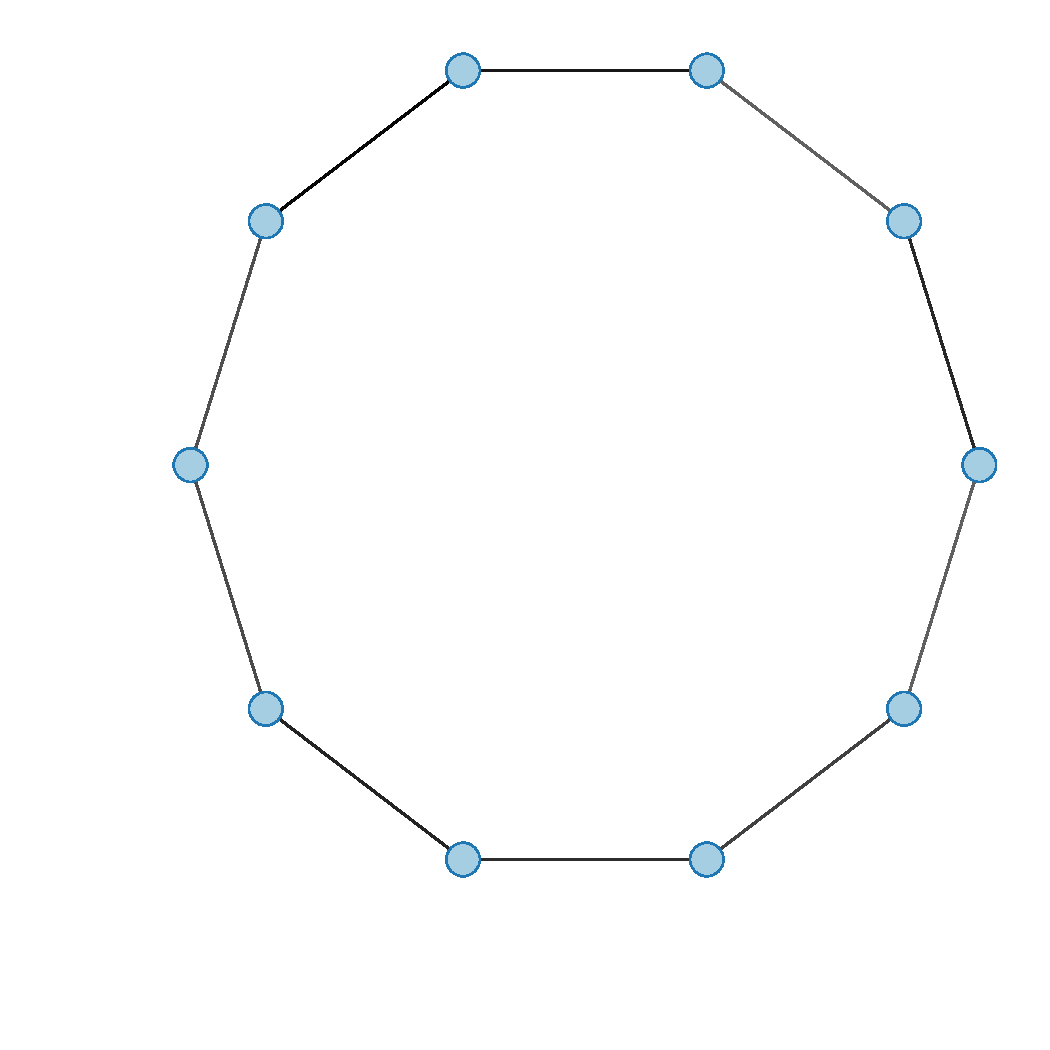
\includegraphics[width=1\textwidth]{imgs/minimallyConnected.pdf}
                \caption{Low $\bar{k}$}
                \label{fig:minimallyConnected}
        \end{subfigure}%%

\caption[Network topologies used to test whether network connectedness influences pathogen invasion]{The two network topologies used to test whether network connectedness influences a viruses ability to invade. Dispersal is held constant between the two topologies.}
\label{f:net}
\end{figure}






%%%%%%%%%%%%%%%%%%%%%%%%%%%%%%%%%%%%%%%%%%%%%%%%%%%%%%%%%%%%%%%%%%%%%%%%%%%%%%%%%%%%%%%%%%%%%%%%%%%%%%%%%%%%%%%%%%%%%%%%%%%%%%%%%%%%%%%%%%%%%%%%%%%%%%%%%%%

\clearpage
\section{Results}

%%%%%%%%%%%%%%%%%%%%%%%%%%%%%%%%%%%%%%%%%%%%%%%%%%%%%%%%%%%%%%%%%%%%%%%%%%%%%%%%%%%%%%%%%%%%%%%%%%%%%%%%%%%%%%%%%%%%%%%%%%%%%%%%%%%%%%%%%%%%%%%%%%%%%%%%%%%




\subsection{Dispersal}
%%%%%%%%%%%%%%%%%%%%%%%%%%%%%%


The proportion of invasions was not different across dispersal rates. This was true at all transmission levels ($\chi^2$ test. $\beta = 2$: $\chi^2 = 4.19$, $df = 2$, $p = 0.12$. $\beta = 5$: $\chi^2 = 1.27$, $df = 2$, $p = 0.53$. $\beta = 10$: $\chi^2 = 0.01$, $df = 2$, $p = 0.996$)


\begin{figure}[b]
\centering
        \begin{subfigure}[b]{0.35\textwidth}
                \centering
		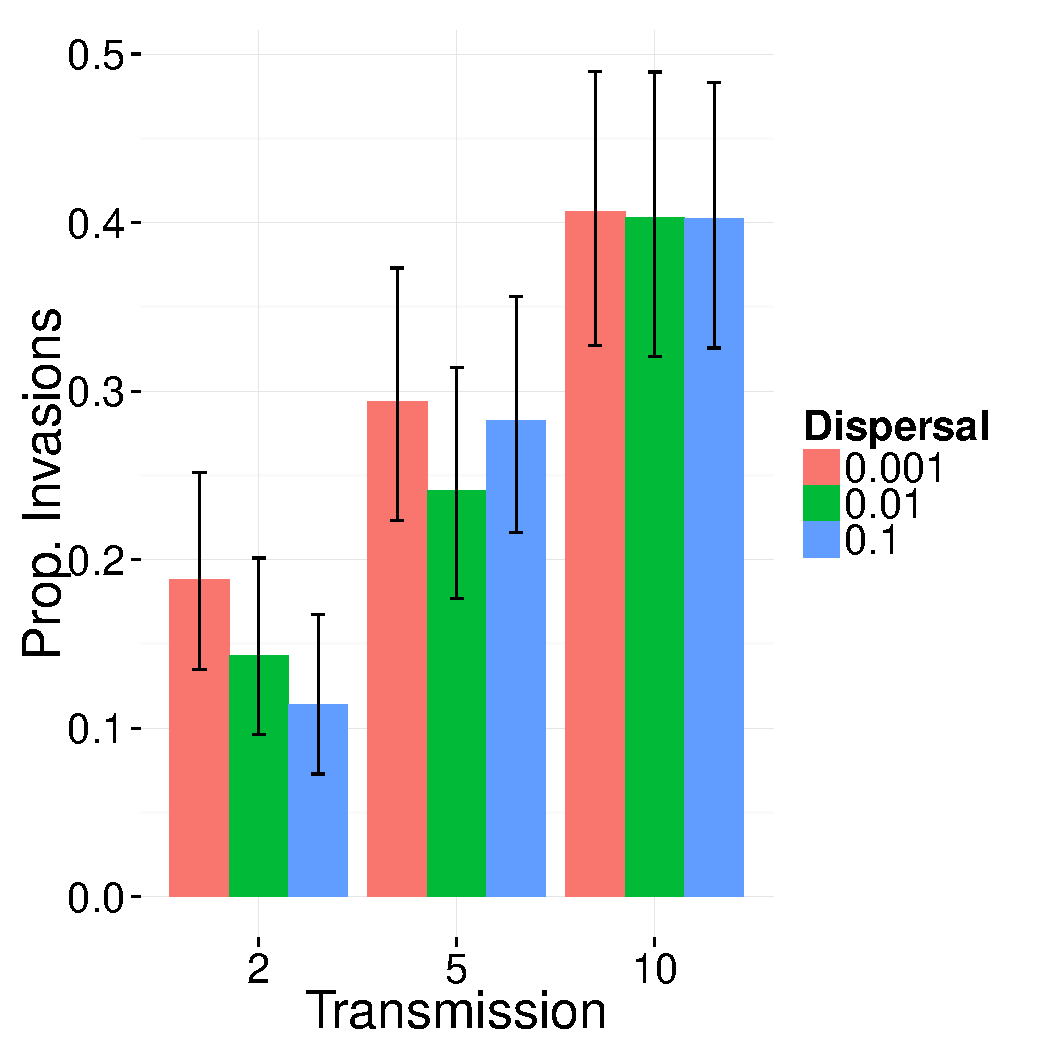
\includegraphics[width=1\textwidth]{imgs/fig150327.pdf}
                \caption{}
                \label{fig:dispersalProbs}
        \end{subfigure}
        ~ 
	\begin{subfigure}[b]{0.35\textwidth}
                \centering
		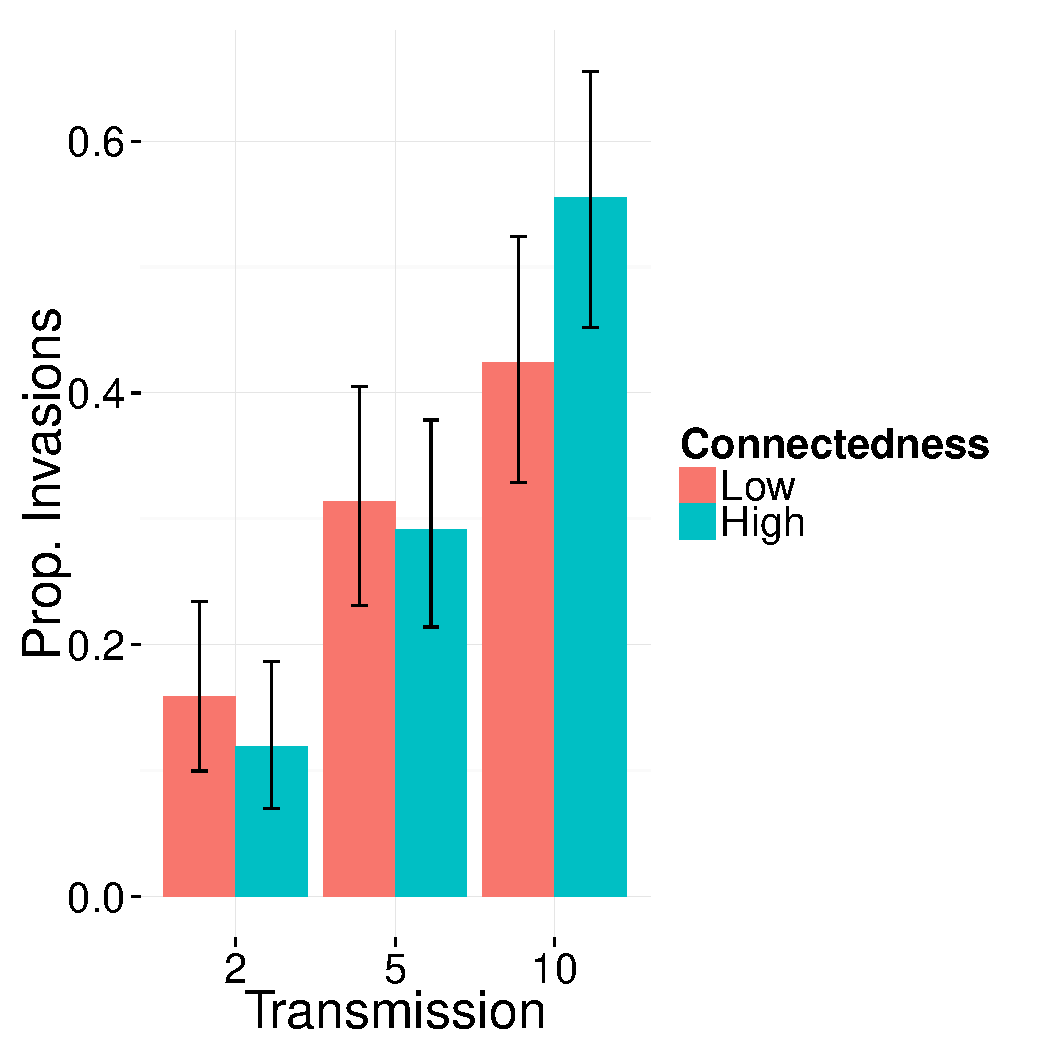
\includegraphics[width=1\textwidth]{imgs/figs.pdf}
                \caption{}
                \label{fig:structureProbs}
        \end{subfigure}%%

\caption[Invasion probability]{The probability of successful invasion. For three different transmission rates, the probability of invasion success does not change between different a) dispersal rates or b) network structures. Error bars are 95\% confidence intervals. Other parameters are kept constant at: $N = 10,\, \bar{n} = 3000,\, b = d = 0.05,\, \gamma = 0.1,\, \alpha = 0.1$. When dispersal is varied, the population structure is fully connected. When population structure is varied, $\lambda = 0.01$.}
\label{f:dist}
\end{figure}


\subsection{Network structure}
%%%%%%%%%%%%%%%%%%%%%%%%%%%%%%

The proportion of invasions was not different between highly connected and largely unconnected metapopulations. This was true at all transmission levels ($\chi^2$ test. $\beta = 2$: $\chi^2 = 0.54$, $df = 1$, $p = 0.46$. $\beta = 5$: $\chi^2 = 0.06$, $df = 1$, $p = 0.81$. $\beta = 10$: $\chi^2 = 3.01$, $df = 1$, $p = 0.08$)

 




%%%%%%%%%%%%%%%%%%%%%%%%%%%%%%%%%%%%%%%%%%%%%%%%%%%%%%%%%%%%%%%%%%%%%%%%%%%%%%%%%%%%%%%%%%%%%%%%%%%%%%%%%%%%%%%%%%%%%%%%%%%%%%%%%%%%%%%%%%%%%%%%%%%%%%%%%%%

\clearpage
\section{Discussion}

%%%%%%%%%%%%%%%%%%%%%%%%%%%%%%%%%%%%%%%%%%%%%%%%%%%%%%%%%%%%%%%%%%%%%%%%%%%%%%%%%%%%%%%%%%%%%%%%%%%%%%%%%%%%%%%%%%%%%%%%%%%%%%%%%%%%%%%%%%%%%%%%%%%%%%%%%%%




%%%%%%%%%%%%%%%%%%%%%%%%%%%%%%%%%%%%%%%%%%%%%%%%%%%%%%%%%%%%%%%%%%%%%%%%%%%%%%%%%%%%%%%%%%%%%%%%%%%%%%%%%%%%%%%%%%%%%%%%%%%%%%%%%%%%%%%%%%%%%%%%%%%%%%%%%%%

\clearpage
\section{Appendix}

%%%%%%%%%%%%%%%%%%%%%%%%%%%%%%%%%%%%%%%%%%%%%%%%%%%%%%%%%%%%%%%%%%%%%%%%%%%%%%%%%%%%%%%%%%%%%%%%%%%%%%%%%%%%%%%%%%%%%%%%%%%%%%%%%%%%%%%%%%%%%%%%%%%%%%%%%%%

\begin{table}[b!]

\begin{tabular}{lp{5.6cm}p{4.3cm}l}
 & Explanation & Units&Value\\
\hline
$S$ & Susceptible individuals &&\\
$I_q$ & Infectious with diseases $q$ &&\\
$I^+_p$ & Sum of classes infected with pathogen $p$ &\\
$N$ & Number of colonies&& 10\\
$\bar{n}$ & Mean colony starting size && 3000\\
$\beta$ & Transmission rate & Transmission events per year per individual& 2, 5, 10\\
$\gamma$ & Recovery rate & Recovery events per year. & 0.1\\
$\lambda$ & Dispersal & Dispersal events per day per individual& 0.001--0.1\\
$b$ & Birth rate & Births per year per individual& 0.05\\
$d$ & Death rate & Deaths per year per individual & 0.05\\
$d_I$ & Infectious death rate & Additional deaths per day per individual&\\
$\rho$ & No. pathogens && 2\\
$p$ &  Pathogen index i.e. $p\in\{1,2\}$ for pathogens 1 and 2 & &\\
$q$ & Disease class i.e., $q\in\{1,2,12\}$&\\
$\mathcal{V}$ & Neighourhood of a node &&\\
$t, t^\prime$ & Time and time plus waiting time i.e., $t+\delta$ & Days&\\
$k_i$ & Degree of node $i$ &&\\
$\delta$ & Waiting time until next event & Days&\\
$\alpha$ & Cross immunity & Proportion& 0.1\\
$n, m$ & Colony index &&\\
$\bm{A}_{mn}$ & Adjacency matrix. & Distance &\\
$\mu$ & Maximum distance for edge to exist & km& 40, 100\\
$\sigma$ & Invading pathogen seed size & & 10\\
$r_i$ & The rate that event $i$ occurs. & Days$^{-1}$&\\
&&&\\
\end{tabular}
\caption{All symbols used.}
\label{t:params}
\end{table}







\chapter{Does ecological and epidemiological seasonality promote viral diversity?}
\label{chapterlabel3}
\clearpage







\section{Abstract}


\tmpsection{One or two sentences providing a basic introduction to the field}
% comprehensible to a scientist in any discipline.
\lettr{B}ats are an important reservoire of zoonotic diseases.
It is still unclear what factors determine the number of pathogens a wild bat species carries.
But once understood, these factors could provide a way to priorities surveillance of bat populations.


\tmpsection{Two to three sentences of more detailed background}
% comprehensible to scientists in related disciplines.


\tmpsection{One sentence clearly stating the general problem (the gap)}
% being addressed by this particular study.


\tmpsection{One sentence summarising the main result}
%  (with the words “here we show” or their equivalent).


\tmpsection{Two or three sentences explaining what the main result reveals in direct comparison to what was thought to be the case previously}
% or how the main result adds to previous knowledge


\tmpsection{One or two sentences to put the results into a more general context.}



\tmpsection{Two or three sentences to provide a broader perspective, }
% readily comprehensible to a scientist in any discipline.



%%%%%%%%%%%%%%%%%%%%%%%%%%%%%%%%%%%%%%%%%%%%%%%%%%%%%%%%%%%%%%%%%%%%%%%%%%%%%%%%%%%%%%%%%%%%%%%%%%%%%%%%%%%%%%%%%%%%%%%%%%%%%%%%%%%%%%%%%%%%%%%%%%%%%%%%%%%

\clearpage
\section{Introduction}

%%%%%%%%%%%%%%%%%%%%%%%%%%%%%%%%%%%%%%%%%%%%%%%%%%%%%%%%%%%%%%%%%%%%%%%%%%%%%%%%%%%%%%%%%%%%%%%%%%%%%%%%%%%%%%%%%%%%%%%%%%%%%%%%%%%%%%%%%%%%%%%%%%%%%%%%%%%





%%%%%%%%%%%%%%%%%%%%%%%%%%%%%%%%%%%%%%%%%%%%%%%%%%%%%%%%%%%%%%%%%%%%%%%%%%%%%%%%%%%%%%%%%%%%%%%%%%%%%%%%%%%%%%%%%%%%%%%%%%%%%%%%%%%%%%%%%%%%%%%%%%%%%%%%%%%

%\clearpage
\section{Methods}

%%%%%%%%%%%%%%%%%%%%%%%%%%%%%%%%%%%%%%%%%%%%%%%%%%%%%%%%%%%%%%%%%%%%%%%%%%%%%%%%%%%%%%%%%%%%%%%%%%%%%%%%%%%%%%%%%%%%%%%%%%%%%%%%%%%%%%%%%%%%%%%%%%%%%%%%%%%

























































To measure pathogen richness I used data from \cite{luis2013comparison}. 
These simply include known infections of a bat species with a pathogen species. 
Only species with at least one pathogen were included in the analysis.
Rows with host species that were not identified to species level were removed.
Many viruses were not identified to species level or their identified species was not in the ICTV virus taxonomy \cite{ICTV}.
I counted a virus if it was the only virus, for that host species, in the lowest taxonomic level identified in the ICTV taxonomy.
That is, if a host carries an unknown Paramyxoviridae virus, then it must carry at least one Paramyxoviridae virus.
If a host carries an unknown Paramyxoviridae virus and a known Paramyxoviridae virus, then it is hard to confirm that the unknown virus is not another record of the known virus.
In this case, this would be counted as one virus species.






\begin{knitrout}\footnotesize
\definecolor{shadecolor}{rgb}{0.969, 0.969, 0.969}\color{fgcolor}\begin{figure}[t]

{\centering 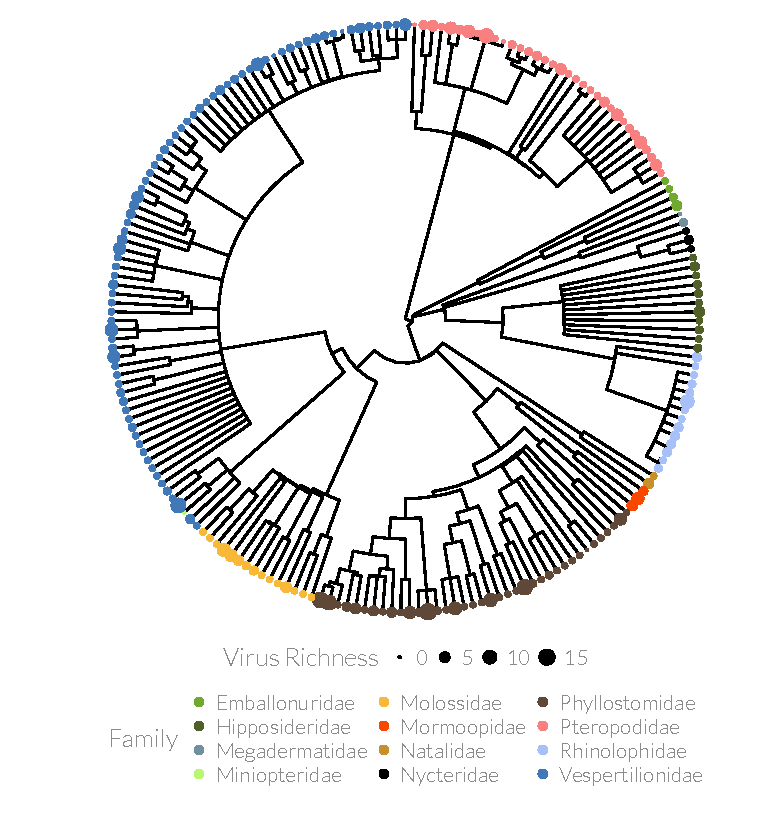
\includegraphics[width=\textwidth]{figure/treePlot-1} 

}

\caption[Pruned phylogeny with dot size showing number of pathogens and colour showing family]{Pruned phylogeny with dot size showing number of pathogens and colour showing family.}\label{fig:treePlot}
\end{figure}


\end{knitrout}












I used two measures of population structure. 
$F_{ST}$ and the number of subspecies.
The number of subspecies was counted using the Wilson and Reeder taxonomy \cite{wilson2005mammal}.
$F_{ST}$ and other measures were collated from the literature.
Studies are from a wide range of spatial scales, from local ($\sim\SI{10}{\kilo\metre}$) to continental.
As $F_{ST}$ inevitably increases with spatial scale I controlled for this by only using data from studies where a large proportion of the species range was studied.
I used the ratio of the furthest distance between $F_{ST}$ samples to the width of the species range and only used studies if this ratio was greater than 0.3.
To allow comparison between different measures ($F_{ST}, \phi_{ST}$) and data from different molecular regions I converted all data to diploid gene flow.
WILL ADD EXTRA METHODS LATER.
These two measures of population structure were analysed separately as the number of subspecies has 196 data points while there is only $F_{ST}$ data for $\sim 30$ bat species.

To control for study bias I collected the number of Pubmed and Google Scholar citations for each bat species including synonyms from ITIS \cite{itis} via the taxize package \cite{chamberlain2013taxize}.
The counts were scraped using the rvest package \cite{rvest}.
I log transformed these variables as they were strongly right skewed.
The log number of citations on Pubmed and Google scholar were highly correlated (pgls: $t$ = 19.32, df = 194, $p$ = 0).
The results here are for analyses using only Google Scholar citations.
See the appendix for analyses run using Pubmed citations.

Measures of body mass are taken from Pantheria \cite{jones2009pantheria} and primary literature \cite{canals2005relative, arita1993rarity, lopez2014echolocation, orr2013does, , lim2001bat, aldridge1987turning, ma2003dietary, owen2003home, henderson2008movements, heaney2012nyctalus, oleksy2015high, zhang2009recent}. 
\emph{Pipistrellus pygmaeus} was assigned the same mass as \emph{P. pipistrellus} as they indistinguishable by mass.
Body mass measurements were log transformed due to the strong right skew.
Distribution size was estimated by downloading range maps for all species from IUCN \cite{} and were also logged due to right skew.

%Pubmed was scraped on pubmedScrapeDate and Google Scholar was scraped on scholarScrapeDate

To control for phylogenetic nonindependance I used the best-supported phylogeny from \cite{fritz2009geographical} which is the supertree from \cite{bininda2007delayed} with names updated to match the Wilson \& Reeder taxonomy \cite{wilson2005mammal}.
Phylogenetic manipulation was performed using the ape package \cite{ape}.
The importance of the phylogeny on each variable separately was estimated using \cite{phytools}.








%\clearpage







\begin{knitrout}\footnotesize
\definecolor{shadecolor}{rgb}{0.969, 0.969, 0.969}\color{fgcolor}\begin{figure}[t]

{\centering 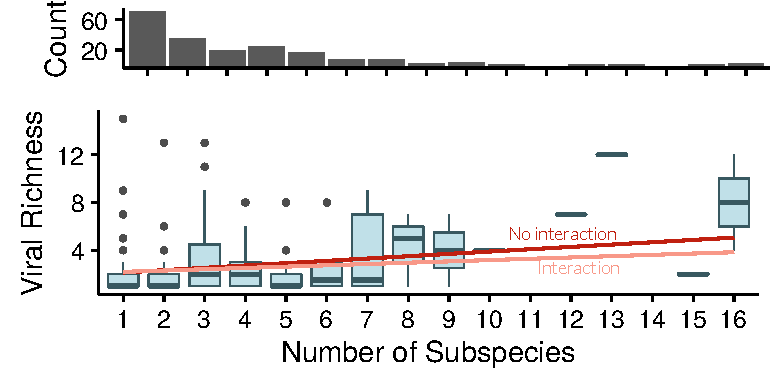
\includegraphics[width=0.8\textwidth]{figure/boxplot-1} 

}

\caption[Number of virus species against number of subspecies]{Number of virus species against number of subspecies. 
Data within a number of subspecies are plotted as boxplots with the dark bar showing the median, the box showing the interquartile range, vertical lines showing the range and outliers shown as seperate points.
Regression lines are from multivariate phylogenetic models with other independant variables set at their median value.
The models shown are thos with (pink) and without (red) an interaction between study effort and number of subspecies.
}\label{fig:boxplot}
\end{figure}


\end{knitrout}









\begin{knitrout}\footnotesize
\definecolor{shadecolor}{rgb}{0.969, 0.969, 0.969}\color{fgcolor}\begin{figure}[t]

{\centering 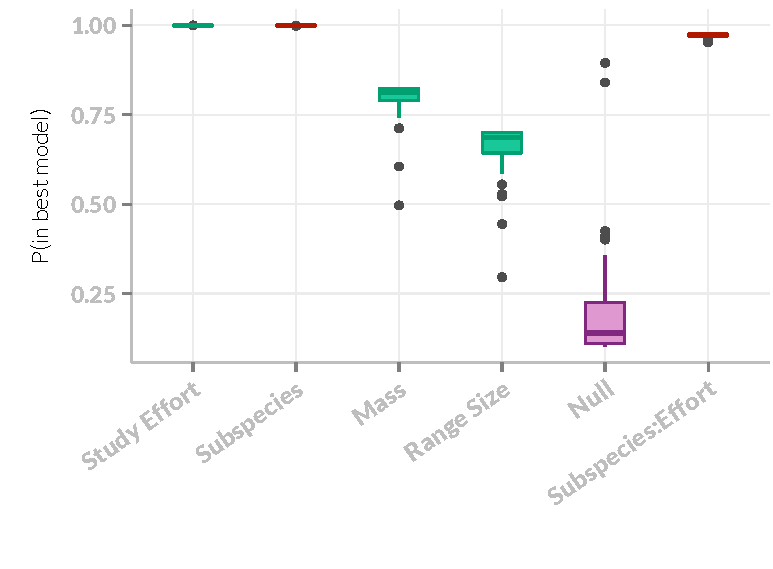
\includegraphics[width=0.8\textwidth]{figure/ITPlots-1} 

}

\caption[Akaika variable weights for number of subspecies analysis]{Akaika variable weights for number of subspecies analysis. The probability that each variable will be in the best model if the data were recollected is shown for each of the bootstrap analyses. The purple ``Null'' box is a uniform random variable used as a null. Population structure (Number of subspecies) and the interaction between subspecies and study effort, shown in red, are more likely to be in the best model than this random variable.}\label{fig:ITPlots}
\end{figure}


\end{knitrout}






\clearpage





%%%%%%%%%%%%%%%%%%%%%%%%%%%%%%%%%%%%%%%%%%%%%%%%%%%%%%%%%%%%%%%%%%%%%%%%%%%%%%%%%%%%%%%%%%%%%%%%%%%%%%%%%%%%%%%%%%%%%%%%%%%%%%%%%%%%%%%%%%%%%%%%%%%%%%%%%%%
%%%% FST ANALYSIS                                                                                                                                  %%%%%%%%
%%%%%%%%%%%%%%%%%%%%%%%%%%%%%%%%%%%%%%%%%%%%%%%%%%%%%%%%%%%%%%%%%%%%%%%%%%%%%%%%%%%%%%%%%%%%%%%%%%%%%%%%%%%%%%%%%%%%%%%%%%%%%%%%%%%%%%%%%%%%%%%%%%%%%%%%%%%






















\begin{knitrout}\footnotesize
\definecolor{shadecolor}{rgb}{0.969, 0.969, 0.969}\color{fgcolor}\begin{figure}[t]

{\centering 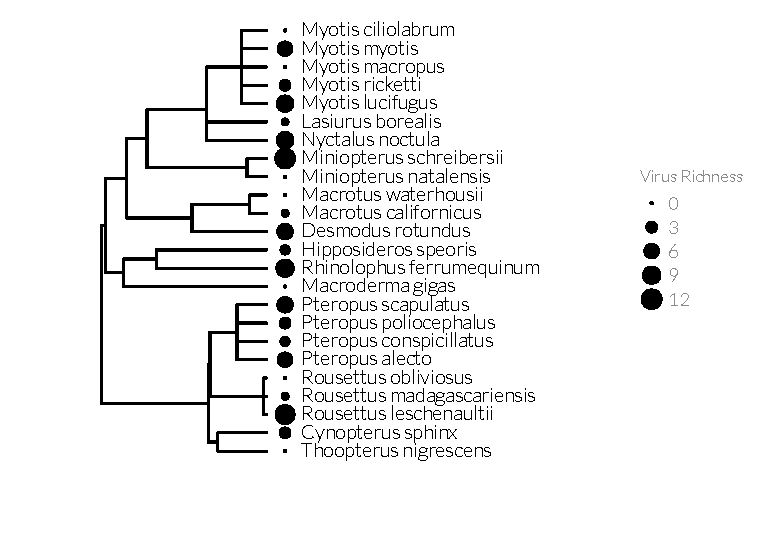
\includegraphics[width=\textwidth]{figure/fstTreePlot-1} 

}

\caption[Pruned phylogeny with dot size showing number of pathogens and colour showing family]{Pruned phylogeny with dot size showing number of pathogens and colour showing family.}\label{fig:fstTreePlot}
\end{figure}


\end{knitrout}

\begin{knitrout}\footnotesize
\definecolor{shadecolor}{rgb}{0.969, 0.969, 0.969}\color{fgcolor}

{\centering 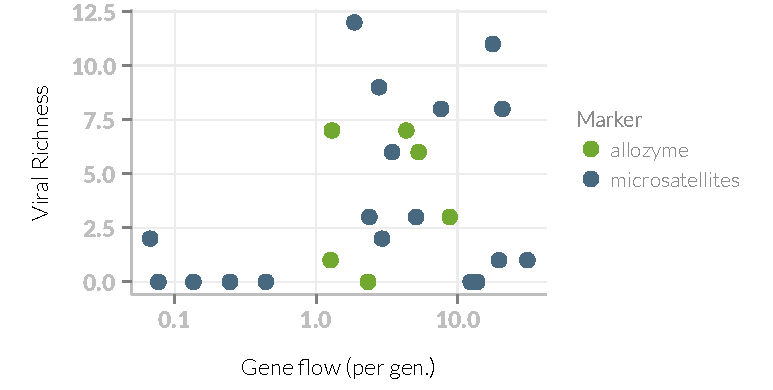
\includegraphics[width=0.8\textwidth]{figure/fstRawData-1} 

}



\end{knitrout}













\begin{knitrout}\footnotesize
\definecolor{shadecolor}{rgb}{0.969, 0.969, 0.969}\color{fgcolor}\begin{figure}[t]

{\centering 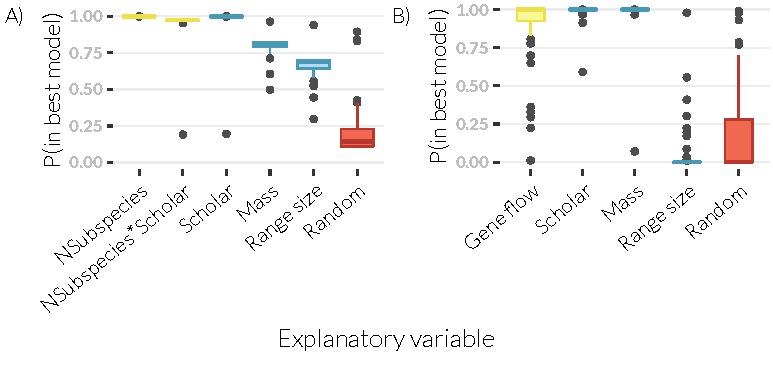
\includegraphics[width=0.8\textwidth]{figure/fstITPlots-1} 

}

\caption{Akaika variable weights for $F_{ST}$ analysis. The probability that each variable will be in the best model if the data were recollected is shown for each of the bootstrap analyses. The purple ``Null'' box is a uniform random variable used as a null. Population structure ($F_{ST}$), shown in red, is much less likely to be in the best model than this random variable.}\label{fig:fstITPlots}
\end{figure}


\end{knitrout}










$F_{ST}$ studies are conducted at a range of spatial scales, but $F_{ST}$ often increases with distance studied \cite{}.
To minimise the effects of this I only used data from studies that cover 20\% of the diameter of the species range.
This is a largely arbitrary value that could be considered to reflect a `global' estimate of $F_{ST}$ while keeping a reasonable number of datapoints available.
I calculated the diameter of the species range by finding the furthest apart points in the IUCN species range \cite{} even if the range is split into multiple polygons.
The width covered by each study was the distance between the most distant sampling sites.
When this was not explicit in the paper, the centre of the lowest level of geographic area was used.



\subsection{Statistical analysis}

Statistical analysis for both dependant variables were conducted using a information theory/model averaging approach \cite{burnham2002model} specifically following \cite{whittingham2005habitat, whittingham2006we}.
I chose a credible set of models including all combinations of independent variables.
In the analysis using the number of subspecies dependant variable I also included an interaction term between study effort and number of subspecies as I believe \emph{a priori} that this interaction may be present.
The interaction was only included in models with both study effort and number of subspecies as an individual term.

I fitted phylogenetic regressions using caper \cite{nmle} to all models.
In each case I simultaneously fitted the $\lambda$ parameter as this avoids mispecifying the model \cite{revell2010phylogenetic}.
$\kappa$ and $\delta$ were constrained to one.

As the number of data points is close to or much less than the number of variables times 40 I calculated small sample corredted AIC (AICc) for each model and then calculated Akaiki weights.
This value can be interpreted as the probability that a model would be the best model if the data were recollected.
For each variable, the sum of the Akaiki weights for models containing that variable are summed.
This value can be interpreted as the probability that the given variable is in the best model.
Following \cite{whittingham2005habitat} I included a uniformally random variable as a null variable as even unimportant variables can have Akaiki weights significantly greater than zero.
The whole analysis was run 50 times, resampling the random variable each time.
We calculated $\bar{AICc}$ by averaging AICc scores within models.
$\Delta\text{AICc}$ was calculated as $\text{min}(\bar{AICc}) - \bar{AICc}$, not the mean of the individual $\Delta\text{AICc}$ scores, to guarantee that the best model has $\Delta\text{AICc} = 0$.


Plots were created with a combination of \cite{ggplot2, palettetown, dotwhisker, ggtree}
%%%%%%%%%%%%%%%%%%%%%%%%%%%%%%%%%%%%%%%%%%%%%%%%%%%%%%%%%%%%%%%%%%%%%%%%%%%%%%%%%%%%%%%%%%%%%%%%%%%%%%%%%%%%%%%%%%%%%%%%%%%%%%%%%%%%%%%%%%%%%%%%%%%%%%%%%%%

\clearpage
\section{Results}

%%%%%%%%%%%%%%%%%%%%%%%%%%%%%%%%%%%%%%%%%%%%%%%%%%%%%%%%%%%%%%%%%%%%%%%%%%%%%%%%%%%%%%%%%%%%%%%%%%%%%%%%%%%%%%%%%%%%%%%%%%%%%%%%%%%%%%%%%%%%%%%%%%%%%%%%%%%

\subsection{Number of Subspecies}
\tmpsection{More descriptive}

After data cleaning there was data for 196 bat species in 11 families.
The number of described virus species for a bat host ranged up to 15 viruses in \emph{Carollia perspicillata}.
Figure~\ref{fig:treePlot} shows the phylogeny used and the number of viruses for each species.
The mean number of viruses across families is fairly constant with a lower range of 1.67 for Nycteridae.
The highest mean is Mormoopidae with 5 virus species per bat species, but this is based on a sample size of 3.
The Phyllostomidae have the second highest mean (n = 37) of 3.49.

The small change in mean pathogen richness across families and the lack of clear pattern in Figure~\ref{fig:treePlot} implies that viral richness is not strongly phylogenetic. 
This is corroborated by the small estimated size of $\lambda$ ($\lambda$ = , $p$ = ).
This fact implies that other factors must control pathogen richness.
It also implies that pathogens are not directly inherited down the phylogeny, although this is to be expected by the fast evolution of viruses.

Of the explanatory variables, the number of subspecies has no phylogenetic autocorrelation ($\lambda$ = , $p$ = ), study effort has weak but significant autocorrelation ($\lambda$ = , $p$ = ) and mass is strongly phylogenetic ($\lambda$ = , $p$ = ).

\tmpsection{Model results}
%See Figure \ref{fig:plotSubspeciesCoefs} for a display of estimated coefficients for the two models using number of viruses as the response variable. 
The main model with mass, study effort and number of subspecies as predictors found study effort to be highly significant ($\beta = $ NA, $p = $ \ensuremath{1.05\times 10^{-8}}). 
The number of subspecies was marginally significant ($\beta = $ NA, $p = $ 0.02). 
The effect of nonindependance due to phylogeny was very small ($\lambda = $ 0.09, $p = $ 0.02).

The interaction term between study effort and number of subspecies, when included, was significant ($\beta = $ 0.14, $p = $ \ensuremath{2.99\times 10^{-3}}).



\subsection{$F_{ST}$}











%\begin{table}[t]
%  \rowcolors{2}{gray!25}{white}
%  \begin{tabular}{lrr}
% \hline
%  Covariate & Estimate (95\% CI) & $p$ value\\
%  \hline
%  Number of subspecies & tableM[2,1] (tableM[2, 2] -- tableM[2, 3]) & tableM[2, 4]\\
%  Mass & tableM[3,1] (tableM[3, 2] -- tableM[3, 3]) & tableM[3, 4]\\
%  Study effort & tableM[4,1] (tableM[4, 2] -- tableM[4, 3]) & tableM[4, 4]\\
%  Intercept & tableM[1,1] (tableM[1, 2] -- tableM[1, 3]) & tableM[1, 4]\\
%  \end{tabular}
%\caption{Table of parameter estimates.}
%\label{t:params}
%\end{table}


\begin{table}[t]
\rowcolors{2}{gray!25}{white}
\begin{tabular}{>{\small}lrrrr}

\normalsize{Model} & $\bar{\text{AICc}}$ & $\Delta$AICc & $w_i$ & $\sum w_i$\\
\hline
log(Scholar)*NSubspecies + rand & 
896 & 0.00 &
0.14 & 0.14\\
log(Scholar)*NSubspecies & 
896 & 0.15 &
0.13 & 0.27\\
log(Scholar)*NSubspecies + rand + log(Mass) & 
896 & 0.15 &
0.13 & 0.40\\
log(Scholar)*NSubspecies  + log(Mass) & 
896 & 0.35 &
0.12 & 0.52\\
log(Scholar)*NSubspecies  + log(Mass) + log(RangeSize) & 
897 & 0.95 &
0.09 & 0.61\\
log(Scholar)*NSubspecies  + rand + log(RangeSize) & 
898 & 2.03 &
0.05 & 0.66\\
log(Scholar)*NSubspecies  + log(RangeSize) & 
898 & 2.15 &
0.05 & 0.71\\
log(Scholar) + NSubspecies & 
898 & 2.35 &
0.04 & 0.75\\
log(Scholar) + NSubspecies + log(Mass) & 
899 & 2.51 &
0.04 & 0.79
\end{tabular}
\caption{
Model selection results. 
$\bar{\text{AICc}}$ is the mean AICc score across 50 resamplings of the null random variable. 
$\Delta$AICc is the $\bar{\text{AICc}}$ score minus the lowest score. 
$w_i$ is the Akaike weight and can be interpreted as the probability that the model is the best model (of those in the plausible set).
$\sum w_i$ is the cumulative sum of the Akaike weights.}
\label{t:subsmodels}
\end{table}




%%%%%%%%%%%%%%%%%%%%%%%%%%%%%%%%%%%%%%%%%%%%%%%%%%%%%%%%%%%%%%%%%%%%%%%%%%%%%%%%%%%%%%%%%%%%%%%%%%%%%%%%%%%%%%%%%%%%%%%%%%%%%%%%%%%%%%%%%%%%%%%%%%%%%%%%%%%

\clearpage
\section{Discussion}  

%%%%%%%%%%%%%%%%%%%%%%%%%%%%%%%%%%%%%%%%%%%%%%%%%%%%%%%%%%%%%%%%%%%%%%%%%%%%%%%%%%%%%%%%%%%%%%%%%%%%%%%%%%%%%%%%%%%%%%%%%%%%%%%%%%%%%%%%%%%%%%%%%%%%%%%%%%%
















\clearpage




















\chapter{Does social structure affect viral diversity in wild bat populations?}
\label{chapterlabel4}











\section{Abstract}


\tmpsection{One or two sentences providing a basic introduction to the field}
% comprehensible to a scientist in any discipline.
\lettr{A}n increasingly large fraction of emerging diseases come from animals \cite{jones2008global, taylor2001risk} and these diseases have a huge impact on human health.
The chance that a new disease will come from any particularly wild host species increases with the diversity of pathogens in that species.
However, the factors that control pathogen diversity in wild populations are still unknown.



\tmpsection{Two to three sentences of more detailed background}
Population density is known to increase pathogen richness while theory suggests that population structure may also play a role.
However, these factors, along with population abundance, are intrinsically linked; reducing density reduces contacts between individuals.
In group living species, this is particularly true, with group size and the number of groups and distribution size contributing to total animal density. 
As these factors are completely interdependant, it is very difficult to study them empirically e.g. in a comparative frame work.

\tmpsection{One sentence clearly stating the general problem (the gap)}
% being addressed by this particular study.

It is unknown whether it is specifically density that controls pathogen diversity or whether density merely correlates with population structure, group size or population size (abundance).


\tmpsection{One sentence summarising the main result}
%  (with the words “here we show” or their equivalent).
Here I use metapopulation SIR models to test whether it is density \emph{per se} that increases the ability of a new pathogen to invade as apposed to colony size, population abundance or population structure.



\tmpsection{Two or three sentences explaining what the main result reveals in direct comparison to what was thought to be the case previously}
% or how the main result adds to previous knowledge



\tmpsection{One or two sentences to put the results into a more general context.}

\tmpsection{Two or three sentences to provide a broader perspective, }
% readily comprehensible to a scientist in any discipline.





%%%%%%%%%%%%%%%%%%%%%%%%%%%%%%%%%%%%%%%%%%%%%%%%%%%%%%%%%%%%%%%%%%%%%%%%%%%%%%%%%%%%%%%%%%%%%%%%%%%%%%%%%%%%%%%%%%%%%%%%%%%%%%%%%%%%%%%%%%%%%%%%%%%%%%%%%%%


\section{Introduction}

%%%%%%%%%%%%%%%%%%%%%%%%%%%%%%%%%%%%%%%%%%%%%%%%%%%%%%%%%%%%%%%%%%%%%%%%%%%%%%%%%%%%%%%%%%%%%%%%%%%%%%%%%%%%%%%%%%%%%%%%%%%%%%%%%%%%%%%%%%%%%%%%%%%%%%%%%%%




\tmpsection{General Intro}
%%%%%%%%%%%%%%%%%%%%%%%%%%%%%%
% A basic introduction to the field,
% comprehensible to a scientist in any discipline.

Zoonotic diseases are an increasingly important source of human infectious diseases \cite{jones2008global, woolhouse2006host, taylor2001risk}.
The diversity of pathogens in wild animal populations is huge and largely unknown \cite{poulin2014parasite}.
The factors that allow large numbers of pathogen species to coexist in a host \cite{anthony2013strategy, anthony2013strategy} are still unclear.
It is likely that population level factors such as population density, range size and population structure have an important role in controlling pathogen community dynamics.
Global change is strongly peturbing wild animal populations, but without clear mechanistic models of how these populations maintain pathogen species richness, we can not predict how pathogen communities, and the risks of zoonotic outbreaks, will change in the coming decades.





\tmpsection{Specific Intro}
%%%%%%%%%%%%%%%%%%%%%%%%%%%%%%
% more detailed background}
% comprehensible to scientists in related disciplines.

\tmpsection{Theoretical background}
Variables that describe populations, such as population density and structure, are well established as having a central role in pathogen dynamics \cite{colizza2007invasion, barthelemy2010fluctuation, colizza2007invasion,  wu2013threshold, may1979population, anderson1979population}.
More recently, the role of the population has been examined with respect to pathogen richness and the coexistence of competing pathogens \cite{qiu2013vector, allen2004sis, nunes2006localized}.
Yet even in theoretical studies there is confusion as to how exactly we should measure populations.
There is disagreement on whether population density (individuals per unit area) should be preferred over population abundance (number of individuals) \cite{begon2002clarification} and how exactly area should be incorporated \cite{begon2002clarification}. 


\tmpsection{Density/abundance in comparative research}
With the increase of novel zoonotic pathogens \cite{} attention has turned to comparatively assessing the factors that are associated with high or low pathogen richness in wild animal species \cite{morand review}.
Here again there is little clarity on the relationship between a number of species measurements.
Population density is commonly studied \cite{} as is range size \cite{}.
However it is rarely if ever acknowledge that these two values are intrinsically linked by $d = N/a$ where $d$ is density, $N$ is the population size and $a$ is area.
In contrast, abundance has never been directly studied as a predictor of pathogen richness.
This is  a glaring omission as abundance more closely aligns with the ``island-biogeography'' class of mechanisms posited to explain pathogen richness \cite{}.
Furthermore, abundance is considered the more relevant measure in terms of pathogen dynamics, especially when area cannot be assumed to be constant \cite{begon} as is commonly the case in wild populations, especially in the face of global warming and habitat degradation.

\tmpsection{Populatiion structure in comparative research}
It is clear that individuals of an animal species are not randomly distributed in space: social groups are common \cite{} and geographic boundaries reduce contacts between isolated populations.
In social species, measures such as global population density are largely meaningless with respect to the number of infectious contacts individuals may have.
Rather, contacts are based on group size and rates of movements between groups.
Two aspects of non-random transmission have been studied in particular: group size \cite{nunn and others} and global measures of population structure including genetic measures and measures derived from distribution shapes (\textcite{gay, maganga, turmelle} and see Chapter \ref{ch:}).
Again however, the relationships between these terms and more the more global terms mentioned above are rarely examined.
Population abundance can be decomposed into two components, the number of groups and the average size of a group with $N = nm$ where $n$ is group size and $m$ is the number of groups.
The amount of movement between is largely dependant on the distance between groups.
This depends on the number of groups per area $m/a$ or $N/na$ and the average distance between groups, if groups are randomly distributed in space scales as $something$.

\tmpsection{But reaction to climate change, and predictions depend on which factor is actually important}


Importantly, these factors, although interrelated, will respond differently to global change and the response will be species dependant.
Some species may suffer large range contractions, and therefore large falls in absolute abundance, while their density remains fairly constant.
Other species might be expected to retain their distribution but have a depressed population density across their range.
Similarly with population structure, species particularly affected by habitat fragmentation can expect increased reduced movement of individuals between groups, while other species may be most affected by a reduction in group size.
Furthermore, different mechanisms of maintenance and creation of pathogen richness will respond to changes in these factors differently as well.
If pathogen richness ultimately depends on the ``island size'' of the host population, then falls in population abundance will reduce pathogen richness the most.
If local group size affects the ability of new pathogens to invade (Chapter \ref{ch:sim1}) then changes in group size are likely to be most important.
Finally, if increased population structure allows pathogens to coexist (\parencite{qiu2013vector, allen2004sis, nunes2006localized} and Chapter \ref{ch:}) increase habitat fragmentation could be expected to increase pathogen richness.

As these factors are likely to be correlated, correlative comparative studies will struggle to distinguish between them.
Furthermore, even if factors are supported or rejected, the specific mechanisms by which the promote pathogen richness will remain unknown, and these may suggest different responses to global change.
Furthermore, mechanistic models are expected to be more predictive into the future and into hitherto unseen parameter space.




\tmpsection{The gap}
%%%%%%%%%%%%%%%%%%%%%%%%%%%%%%

Therefore there is great need to mechanistic models that try to disentangle the interplay between these many factors: density, abundance, range size, population structure, group size and the number of groups.

\tmpsection{What I did and found}
%%%%%%%%%%%%%%%%%%%%%%%%%%%%%%


% One sentence summarising the main result
% (with the words “here we show” or their equivalent).








%%%%%%%%%%%%%%%%%%%%%%%%%%%%%%%%%%%%%%%%%%%%%%%%%%%%%%%%%%%%%%%%%%%%%%%%%%%%%%%%%%%%%%%%%
%%%% Constant density size. 
%%%%%%%%%%%%%%%%%%%%%%%%%%%%%%%%%%%%%%%%%%%%%%%%%%%%%%%%%%%%%%%%%%%%%%%%%%%%%%%%%%%%%%%%%







%%%%%%%%%%%%%%%%%%%%%%%%%%%%%%%%%%%%%%%%%%%%%%%%%%%%%%%%%%%%%%%%%%%%%%%%%%%%%%%%%%%%%%%%%
%%%% Constant density 2. 
%%%%%%%%%%%%%%%%%%%%%%%%%%%%%%%%%%%%%%%%%%%%%%%%%%%%%%%%%%%%%%%%%%%%%%%%%%%%%%%%%%%%%%%%%









%%%%%%%%%%%%%%%%%%%%%%%%%%%%%%%%%%%%%%%%%%%%%%%%%%%%%%%%%%%%%%%%%%%%%%%%%%%%%%%%%%%%%%%%%
%%%% Constant Population. 
%%%%%%%%%%%%%%%%%%%%%%%%%%%%%%%%%%%%%%%%%%%%%%%%%%%%%%%%%%%%%%%%%%%%%%%%%%%%%%%%%%%%%%%%%








\begin{knitrout}\footnotesize
\definecolor{shadecolor}{rgb}{0.969, 0.969, 0.969}\color{fgcolor}\begin{figure}[t]

{\centering 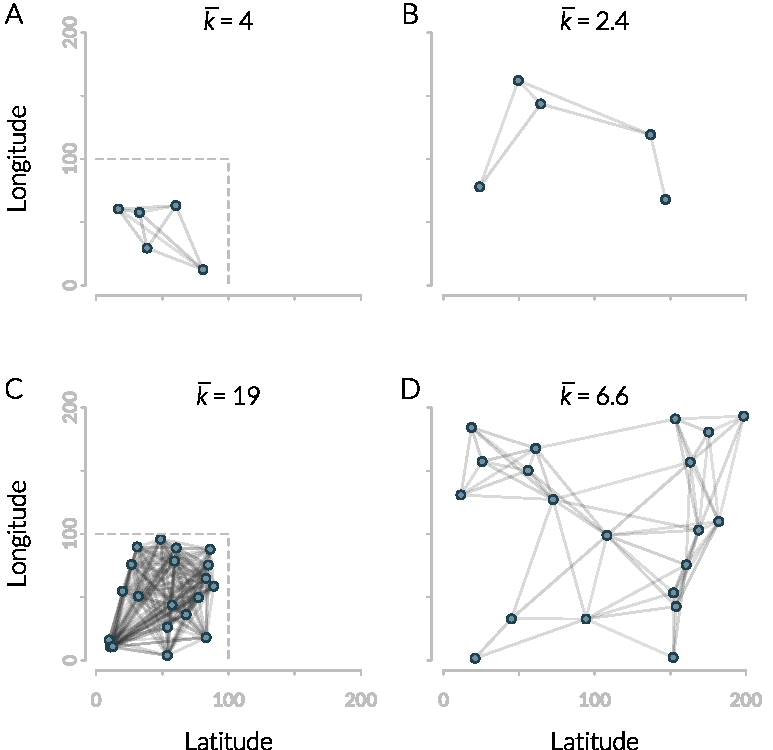
\includegraphics[width=0.9\textwidth]{figure/colonyNetworkPlots-1} 

}

\caption[Example metapopulation networks]{
Examples of the metapopulation networks used.
They show the smallest number of colonies (five) and the default (20).
They also show the default ($10^4\,\text{km}^2$, grey dashed lines) and largest areas ($4\times10^4\,\text{km}^2$, full plot), though all networks are plotted on the largest area.
As area increases, the number of connections each subpopulation has decreases as seen by the changes in mean degree, $\bar{k}$.
}\label{fig:colonyNetworkPlots}
\end{figure}


\end{knitrout}




%%%%%%%%%%%%%%%%%%%%%%%%%%%%%%%%%%%%%%%%%%%%%%%%%%%%%%%%%%%%%%%%%%%%%%%%%%%%%%%%%%%%%%%%%%%%%%%%%%%%%%%%%%%%%%%%%%%%%%%%%%%%%%%%%%%%%%%%%%%%%%%%%%%%%%%%%%%


\section{Methods}

%%%%%%%%%%%%%%%%%%%%%%%%%%%%%%%%%%%%%%%%%%%%%%%%%%%%%%%%%%%%%%%%%%%%%%%%%%%%%%%%%%%%%%%%%%%%%%%%%%%%%%%%%%%%%%%%%%%%%%%%%%%%%%%%%%%%%%%%%%%%%%%%%%%%%%%%%%%

%%




\subsection{Metapopulation model}

\tmpsection{Overview}


I used two-pathogen, metapopulation SIR model to compare the roles of demograhic parameters on pathogen species richness.
Specifically I let two identical pathogens (and endemic pathogen and an invading pathogen) compete.
I used presistence or not of the second pathogen as my response variable.
I test whether population abundance is more important than population density.
I then test whether colony size or the number of colonies is the more important component of population abundance.
The multpathogen SIR model is identical to that in Chapter \ref{ch:sims1} and is implemented in R \cite{R}.



In each simulation the population is seeded with 20 individuals infected with pathogen 1 in each colony. 
Pathogen 1 is then allowed to spread and reach equilibrium. 
After \ensuremath{7\times 10^{5}} events, 5 individuals infected with pathogen 2 are added to one colony. 
After another \ensuremath{3\times 10^{5}} events the invasion of pathogen 2 is considered successful if any individuals with pathogen 2 still remain.

\subsection{Dependant variables}

Three dependant variables were varied: colony size, number of colonies and area.
From these parameters, population abundance and population density can be calculated.
The default values of these parameters was a population size of 8000 individuals split into 20 colonies of 400.
The default area of the simulations was 

Three sets of simulations were run.
First, colony size was varied using values 100, 200, 400, 800 and \ensuremath{1.6\times 10^{3}}.
The number of colonies was kept constant and so population abundance varied with colony size.
Area was scaled to keep population density constant. 
Secondly, number of colonies (and therefore population abundance) was varied and again area was varied to keep density constant.
5, 10, 20, 40 and 80 colonies were used.
Finally, colony size and number of colonies were kept constant (therefore keeping population abundance constant) and area was varied alone to alter population density. 
The values of area used were \ensuremath{4\times 10^{4}}, \ensuremath{2\times 10^{4}}, \ensuremath{10^{4}}, \ensuremath{5\times 10^{3}} and \ensuremath{2.5\times 10^{3}} which gave density values of 0.2, 0.4, 0.8, 1.6 and 3.2.

The affects of area occur through changing the metapopulation network.
The metapopulation structure was created for each simulation by randomly placing colonies in space.
The spatial scale of the simulations vary between \ensuremath{2.5\times 10^{3}} and \ensuremath{4\times 10^{4}} km$^2$ (space is given in kilometers even though they are oin fact arbitrary units for simplicity).
This corresponds to square areas with sides of 50 to 200 km).
Dispersal can only occur between two colonies if they are within 100 kilometers of each other i.e. they are connected nodes in the metapopulation network.
The number of connections each colony has is called its degree, $k$.
How well connected the metapopulation network is overall is measured by the mean degree, $\bar{k}$.
This does not guarentee that the population is fully connected but as the endemic pathogen is seeded in all colonies, the invading pathogen cannot be seeded into a fully susceptible colony.
This was considered more realistic than repeatedly resampling the population until a fully connected population occured.
Given this setup, simulations with low densities had relatively unconnected metapopulation networks.






\subsection{Other Parameters}
%TODO switch all b's to d or something else, so that b can be used for regression coeficients. In all eqns in +ch2 as well.

The fixed parameters used are chosen to roughly reflect realistic wild bat populations. 
The death rate $\Lambda$ is set as 0.05 per year giving a generation time of 20 years.
The birth rate is set to be equal to $\mu$ so that the population size is stable.
The recovery rate $\gamma$ is set to 1 giving a average infection duration of 1 years. 
This is therefore a long lasting infection but not a chronic infection. 
It is very difficult to directly estimate infection durations in wild populations but it seems that these infections might sometimes be long lasting \cite{peel2012henipavirus, plowright2015ecological}.
However, other studies have found much shorter infectious periods \cite{amengual2007temporal}.
These shorter lived in infections are studied further here as preliminary simulations found that they could not persist in the relatively small populations being modelled here.

Cross immunity is set to 0.1 so that an individual infected with one pathogen is 90\% less likely to be infected with another.
This is a rather arbitrary value.
However, the rationale of the model is that the invading species might be a newly speciated strain of the endemic species.
Furthermore, the model assumes complete cross immunity after recovery from infection.
Therefore cross immunity to coinfection is likely to be very strong as well.


The population size of each subpopulation is set to 3,000. 
This is appropriate for many bat species \cite{jones2009pantheria}, especially the large, frugivorous \emph{Pteropodidae} that have been particularly associated with recent zoonotic diseases.


Three values of the transmission rate $\beta$ are used, 0.1, 0.2 and 0.3.
All simulations are run under all three transmission rates as this is a fundamental parameter that changes the broad dynamics of the pathogens.


\subsection{Statistical comparisons}

I tested two hypotheses.
Firstly I tested the hypothesis that an increase in population abundance creates a stronger increase in invasion probability (of the second pathogen) than an equal increase in population density.
Secondly I tested the hypothesis that ana increase in colony size creates a stronger increase in invasion probability an an equal increase in number of colonies.
To statistically test these hypotheses I combined the results from different simulations and fitted multiple logistic regressions, centering and scaling the dependant variables.
Specifically, I fitted the model $\text{invasion} = b_1 \text{density} + b_2 \text{colony size} + b_3 \text{number of colonies} + c + \epsilon$ where $c$ is a fitted intercept and $\epsilon$ is a binomially distributed error term.
To test the first hypothesis I compared the size (and 95\% confidence intervals) of $b_1$ to $b_2$ and $b_3$.
To test the second hypothesis I compared $b_2$ to $b_3$.








%%%%%%%%%%%%%%%%%%%%%%%%%%%%%%%%%%%%%%%%%%%%%%%%%%%%%%%%%%%%%%%%%%%%%%%%%%%%%%%%%%%%%%%%%%%%%%%%%%%%%%%%%%%%%%%%%%%%%%%%%%%%%%%%%%%%%%%%%%%%%%%%%%%%%%%%%%%


\section{Results}

%%%%%%%%%%%%%%%%%%%%%%%%%%%%%%%%%%%%%%%%%%%%%%%%%%%%%%%%%%%%%%%%%%%%%%%%%%%%%%%%%%%%%%%%%%%%%%%%%%%%%%%%%%%%%%%%%%%%%%%%%%%%%%%%%%%%%%%%%%%%%%%%%%%%%%%%%%%






















\begin{knitrout}\footnotesize
\definecolor{shadecolor}{rgb}{0.969, 0.969, 0.969}\color{fgcolor}\begin{figure}[t]

{\centering 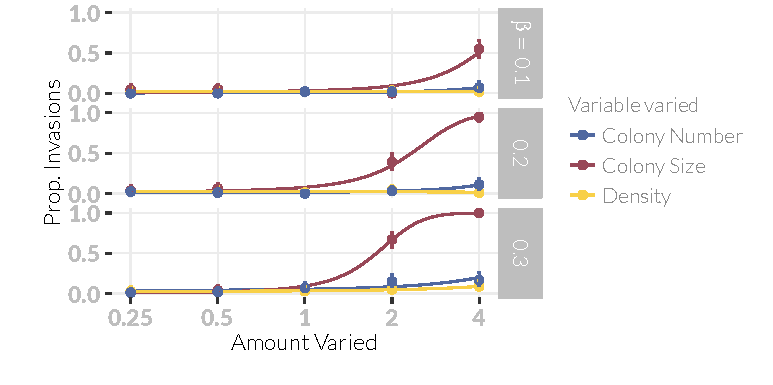
\includegraphics[width=\textwidth]{figure/plotValueChangeMeans-1} 

}

\caption[Comparison of the probability of invasion when population size is altered by changing colony size or colony number.]{
Comparison of the effect of colony size, colony number and area on probability of invasion.
Default values are: colony number = 20, colony size = 400 and density = 0.8 animals per unit area.
The $x$-axis shows the relative change in each of these values ($\times 0.25, 0.5, 1, 2$ and $4$).
For colony size and number, area is altered  so that density remains constant.
For density, population size is constant at 8,000 and area is altered.
Relationships are shown seperately for each transmission value.
Each point is the mean of 
inline{each} simulations and bars are 95\% confidence intervals.
}\label{fig:plotValueChangeMeans}
\end{figure}


\end{knitrout}





\begin{knitrout}\footnotesize
\definecolor{shadecolor}{rgb}{0.969, 0.969, 0.969}\color{fgcolor}\begin{figure}[t]

{\centering 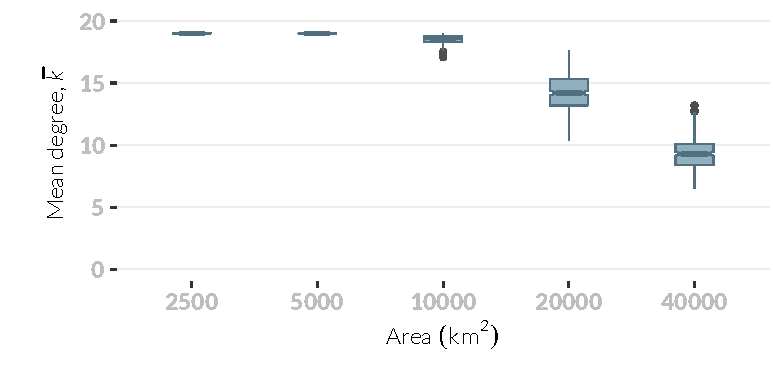
\includegraphics[width=0.8\textwidth]{figure/plotK-1} 

}

\caption[Change in average network degree with increasing area]{
Change in average metapopulation network degree ($\bar{k}$) with increasing area. 
Bars show the median, boxes show the interquartile range, vertical lines show and range and grey dots indicate outlier values.
Notches indicate the 95\% confidence interval of the mean.
}\label{fig:plotK}
\end{figure}


\end{knitrout}





\begin{table}

\caption[Regression results]{
Regression results comparing affects of colony size, colony number and area.
Coefficients are from multiple logistic regressions with invasion as the dependant variable and all independant variables being scaled and centred.
Colony size and colony number were varied while keeping density equal while density was varied by changing area while keeping population size equal.
$p$ is for test against the null hypothesis that  $b = 0$.
}
\label{t:regrCoefs}
\centering
\begin{tabular}{@{}rlrrr@{}}
\toprule
$\beta$ & \emph{Variable} & \emph{Estimate} ($b$) & (95\% \emph{CI}) & $p$\\
\midrule
0.1   &    Intercept     & \ensuremath{-3.52} & (\ensuremath{-3.87}, \ensuremath{-3.2}) & $< 10^{-5}$ \\
      &    Colony Size   & 1.07 & (0.75, 1.49) & $< 10^{-5}$ \\
      &    Colony Number & 0.35 & (\ensuremath{-0.02}, 0.79) & 0.08 \\
      &    Density       & 0.01 & (\ensuremath{-0.66}, 0.52) & 0.97 \\[1em]
0.2   &    Intercept     & \ensuremath{-2.84} & (\ensuremath{-3.12}, \ensuremath{-2.58}) & $< 10^{-5}$ \\
      &    Colony Size   & 2.11 & (1.71, 2.6) & $< 10^{-5}$ \\
      &    Colony Number & 0.51 & (0.16, 0.95) & \ensuremath{9\times 10^{-3}} \\
      &    Density       & \ensuremath{-0.31} & (\ensuremath{-0.96}, 0.19) & 0.29 \\[1em]
0.3   &    Intercept     & \ensuremath{-2.11} & (\ensuremath{-2.34}, \ensuremath{-1.9}) & $< 10^{-5}$ \\
      &    Colony Size   & 2.74 & (2.35, 3.16) & $< 10^{-5}$ \\
      &    Colony Number & 0.25 & (0.04, 0.48) & 0.02 \\
      &    Density       & 0.27 & (\ensuremath{-0.06}, 0.57) & 0.09 \\

\bottomrule



\end{tabular}



\end{table}



%%%%%%%%%%%%%%%%%%%%%%%%%%%%%%%%%%%%%%%%%%%%%%%%%%%%%%%%%%%%%%%%%%%%%%%%%%%%%%%%%%%%%%%%%%%%%%%%%%%%%%%%%%%%%%%%%%%%%%%%%%%%%%%%%%%%%%%%%%%%%%%%%%%%%%%%%%%


\section{Discussion}

%%%%%%%%%%%%%%%%%%%%%%%%%%%%%%%%%%%%%%%%%%%%%%%%%%%%%%%%%%%%%%%%%%%%%%%%%%%%%%%%%%%%%%%%%%%%%%%%%%%%%%%%%%%%%%%%%%%%%%%%%%%%%%%%%%%%%%%%%%%%%%%%%%%%%%%%%%%

\subsection{Restate the gap and the main result}

Empirical studies on the role of population structure on the are equivocal and cannot examine the specific mechanisms by which pathogen communities are created and maintained.
I have used mechanistic, metapopulation models to test whether increased population structure can promote pathogen richness by facilitating invasion of new pathogens.



\subsection{Link results to consequences}

\subsubsection{Population structure does not affect pathogen richness}

Probably because dynamics are dominated by local processes.
This goes against many predictions that increasing $R_0$ increases pathogen richness.
Further work could examine reduced col  ony sizes to test when global structure become more important.
Measures of population structure should not be used to predict zoonotic potential.

\subsubsection{Dispersal does not affect pathogen richness}



\subsubsection{Network connectedness does not affect pathogen richness}

This is in direct contrast to \cite{campos2006pathogen}. 
However, the model in \cite{campos2006pathogen} is a contact network, so increasing the connectedness increases the chance of succesful transmission events for the first few transmission generations.
This lends support to the idea that I found now affect of connectedness due to the dominance of local dynamics.

Network connectedness can be seen as a function of average dispersal distance, density and colony size.
A high density species with small colony sizes must have colonies relatively close together.
Therefore colonies would be more likely to be connected for a given dispersal distance. 


\subsection{Discuss assumptions}

\subsubsection{Complete cross-immunity}

I have assumed that once recovered, individuals are immune to both pathogens. 
Furthermore, when a coinfected individual recovers from one pathogen, it immediately recovers from the other as well.
This is probably a fairly reasonable assumption given that I am modelling a newly evolved strain.
However, further work could relax this assumption using a model similar to \cite{poletto2015characterising} which contains additional classes for `infected with pathogen one, immune to pathogen two' and `infected with pathogen two, immune to pathogen one'.
The model here was formulated such that the study of systems with greater than two pathogens is still computationally feasible while a model such as used in \cite{poletto2015characterising} contains $3^\rho$ classes for a system with $\rho$ pathogen species.
This quickly becomes computationally restrictive.

\subsubsection{Identical strains}

Many papers on pathogen richness have focussed on the evolution of pathogen traits and have considered a trade off between transmission rate and virulence \cite{nowak1994superinfection, nowak1994superinfection} or infectious period \cite{poletto2013host}.
However, here we are interested in host traits.
Therefore we have assumed that pathogen strains are identical.
It is clear however that there are a number of factors that affect pathogen richness and our focus on host population structure does not imply that pathogen traits are not important.



%%%%%%%%%%%%%%%%%%%%%%%%%%%%%%%%%%%%%%%%%%%%%%%%%%%%%%%%%%%%%%%%%%%%%%%%%%%%%%%%%%%%%%%%%%%%%%%%%%%%%%%%%%%%%%%%%%%%%%%%%%%%%%%%%%%%%%%%%%%%%%%%%%%%%%%%%%%


%\section{Appendix}

%%%%%%%%%%%%%%%%%%%%%%%%%%%%%%%%%%%%%%%%%%%%%%%%%%%%%%%%%%%%%%%%%%%%%%%%%%%%%%%%%%%%%%%%%%%%%%%%%%%%%%%%%%%%%%%%%%%%%%%%%%%%%%%%%%%%%%%%%%%%%%%%%%%%%%%%%%%

%\begin{table}[b!]
%
%\begin{tabular}{lp{5.6cm}p{4.3cm}l}
% & Explanation & Units&Value\\
%\hline
%$S$ & Susceptible individuals &&\\
%$I_q$ & Infectious with diseases $q$ &&\\
%$I^+_p$ & Sum of classes infected with pathogen $p$ &\\
%$N$ & Number of colonies&& 10\\
%$\bar{n}$ & Mean colony starting size && 3000\\
%$\beta$ & Transmission rate & Transmission events per year per individual& 2, 5, 10\\
%$\gamma$ & Recovery rate & Recovery events per year. & 0.1\\
%$\lambda$ & Dispersal & Dispersal events per day per individual& 0.001--0.1\\
%$b$ & Birth rate & Births per year per individual& 0.05\\
%$d$ & Death rate & Deaths per year per individual & 0.05\\
%$d_I$ & Infectious death rate & Additional deaths per day per individual&\\
%$\rho$ & No. pathogens && 2\\
%$p$ &  Pathogen index i.e. $p\in\{1,2\}$ for pathogens 1 and 2 & &\\
%$q$ & Disease class i.e., $q\in\{1,2,12\}$&\\
%$\mathcal{V}$ & Neighbourhood of a node &&\\
%$t, t^\prime$ & Time and time plus waiting time i.e., $t+\delta$ & Days&\\
%$k_i$ & Degree of node $i$ &&\\
%$\delta$ & Waiting time until next event & Days&\\
%$\alpha$ & Cross immunity & Proportion& 0.1\\
%$n, m$ & Colony index &&\\
%%$\bm{A}_{mn}$ & Adjacency matrix. & Distance &\\
%$\mu$ & Maximum distance for edge to exist & km& 40, 100\\
%$\sigma$ & Invading pathogen seed size & & 10\\
%$r_i$ & The rate that event $i$ occurs. & Days$^{-1}$&\\
%&&&\\
%\end{tabular}
%\caption{All symbols used.}
%\label{t:params2}
%\end{table}
%
%





\chapter[gREM for estimating animal density]{A generalised random encounter model for estimating animal density with remote sensor data}
\label{chapterlabel5}







  



\section{Abstract}
\lettr{W}ildlife monitoring technology is advancing rapidly and the use of remote sensors such as camera traps and acoustic detectors is becoming common in both the terrestrial and marine environments.
Current methods to estimate abundance or density require individual recognition of animals or knowing the distance of the animal from the sensor, which is often difficult.
A method without these requirements, the random encounter model (REM), has been successfully applied to estimate animal densities from count data generated from camera traps.
However, count data from acoustic detectors do not fit the assumptions of the REM due to the directionality of animal signals.

We developed a generalised REM (gREM), to estimate absolute animal density from count data from both camera traps and acoustic detectors.
We derived the gREM for different combinations of sensor detection widths and animal signal widths (a measure of directionality).
We tested the accuracy and precision of this model using simulations of different combinations of sensor detection widths and animal signal widths, number of captures, and models of animal movement. 

We find that the gREM produces accurate estimates of absolute animal density for all combinations of sensor detection widths and animal signal widths.
However, larger sensor detection and animal signal widths were found to be more precise.
While the model is accurate for all capture efforts tested, the precision of the estimate increases with the number of captures.
We found no effect of different animal movement models on the accuracy and precision of the gREM.  

We conclude that the gREM provides an effective method to estimate absolute animal densities from remote sensor count data over a range of sensor and animal signal widths.
The gREM is applicable for count data obtained in both marine and terrestrial environments, visually or acoustically (e.g., big cats, sharks, birds, echolocating bats and cetaceans).
As sensors such as camera traps and acoustic detectors become more ubiquitous, the gREM will be increasingly useful for monitoring unmarked animal populations across broad spatial, temporal and taxonomic scales. 

\section{Introduction}


The density of animal populations is one of the fundamental measures in ecology and conservation and has important implications for a range of issues, such as sensitivity to stochastic fluctuations \cite{wright1983stochastic} and extinction risk \cite{purvis2000predicting}.
Monitoring animal population changes in response to anthropogenic pressure is becoming increasingly important as humans rapidly modify habitats and change climates \cite{everatt2014trophic}.
Sensor technology, such as camera traps \cite{karanth1995estimating, rowcliffe2008surveys} and acoustic detectors \cite{acevedo2006using, walters2012continental} are widely used to monitor changes in animal populations as they are efficient, relativity cheap and non-invasive, allowing for surveys over large areas and long periods \cite{rowcliffe2008surveys, kessel2014review, walters2013challenges}.
However, converting sampled count data into estimates of density is problematic as detectability of animals needs to be accounted for \cite{anderson2001need}.

Existing methods for estimating animal density often require additional information that is often unavailable.
For example, capture-mark-recapture methods \cite{karanth1995estimating, borchers2014continuous} require recognition of individuals, and distance methods \cite{harris2013applying} require estimates of how far away individuals are from the sensor \cite{barlow2005estimates, marques2011estimating}.
When individuals cannot be told apart, an extension of occupancy modelling can be used to estimate absolute abundance \cite{royle2003estimating}.
However, as the model is originally formulated to estimate occupancy,  count information is simplified to presence--absence data.
Assumptions about the distribution of individuals (e.g.
a poisson distribution) must also be made \cite{royle2003estimating} which may be a poor assumption for nonrandomly distributed species.
Furthermore repeat, independent surveys must be performed and the definition of a site can be difficult, especially for wide-ranging species \cite{mackenzie2005designing}.

%More recently, the development of the random encounter model (REM), a modification of an ideal gas model \cite{yapp1956theory, Hutchinson_Waser_2007}, has enabled animal densities to be estimated from unmarked individuals of a known speed, and with known sensor detection parameters     \cite{rowcliffe2008estimating}.
The REM method has been successfully applied to estimate animal densities from camera trap surveys \cite{zero2013monitoring}.
However, extending the REM method to other types of sensors (e.g., acoustic detectors) is more problematic, because the original derivation assumes a relatively narrow sensor width (up to $\pi/2$ radians) and that the animal is equally detectable irrespective of its heading \cite{rowcliffe2008estimating}. 

Whilst these restrictions are not problematic for most camera trap makes (e.g., Reconyx, Cuddeback), the REM cannot be used to estimate densities from camera traps with a wider sensor width (e.g.
canopy monitoring with fish eye lenses, \cite{brusa2014increasing}).
Additionally, the REM method is not useful in estimating densities from acoustic survey data as acoustic detector angles are often wider than $\pi/2$ radians.  Acoustic detectors are designed for a range of diverse tasks and environments \cite{kessel2014review}, which naturally leads to a wide range of sensor detection widths and detection distances.
In addition to this, calls emitted by many animals are directional \cite{blumstein2011acoustic}, breaking the assumption of the REM method. 

There has been a sharp rise in interest around passive acoustic detectors in recent years, with a 10 fold increase in publications in the decade between 2000 and 2010 \cite{kessel2014review}.
Acoustic monitoring is being developed to study many aspects of ecology, including the interactions of animals and their environments \cite{blumstein2011acoustic, rogers2013density}, the presence and relative abundances of species \cite{marcoux2011local}, biodiversity of an area \cite{depraetere2012monitoring}, and monitoring population trends \cite{walters2013challenges}. 

Acoustic data suffers from many of the problems associated with data from camera trap surveys in that individuals are often unmarked, making capture-mark-recapture methods more difficult to use \cite{marques2013estimating}.
In some cases the distance between the animal and the sensor is known, for example when an array of sensors is deployed and the position of the animal is estimated by triangulation \cite{lewis2007sperm}.
In these situations distance-sampling methods can be applied \cite{buckland2008estimating}.
However, in many cases distance estimation is not possible, for example when single sensors are deployed, a situation typical in the majority of terrestrial acoustic surveys  \cite{buckland2008estimating}.
In these cases, only relative measures of local abundance can be calculated, and not absolute densities.
This means that comparison of populations between species and sites is problematic without assuming equal detectability \cite{schmidt2003count, walters2013challenges}.
Equal detectability is unlikely because of differences in environmental conditions, sensor type, habitat, and species biology. 

In this study, we create a generalised REM (gREM) as an extension to the camera trap model of \cite{rowcliffe2008estimating}, to estimate absolute density from count data from acoustic detectors, or camera traps, where the sensor width can vary from 0 to $2\pi$ radians, and the signal given from the animal can be directional.
We assessed the accuracy and precision of the gREM within a simulated environment, by varying the sensor detection widths, animal signal widths, number of captures and models of animal movement.
We use the simulation results to recommend best survey practice for estimating animal densities from remote sensors. 

\section{Methods}

\subsection{Analytical Model}

The REM presented by \cite{rowcliffe2008estimating} adapts the gas model to count data collected from camera trap surveys.
The REM is derived assuming a stationary sensor with a detection width less than $\pi/2$ radians.
However, in order to apply this approach more generally, and in particular to stationary acoustic detectors, we need both to relax the constraint on sensor detection width, and allow for animals with directional signals.
Consequently, we derive the gREM for any detection width, $ \theta$, between 0 and $2\pi$ with a detection distance $r$ giving a circular sector within which animals can be captured (the detection zone) (Figure~\ref{f:AngleDef}).
Additionally, we model the animal as having an associated signal width $\alpha$ between 0 and $2\pi$  (Figure~\ref{f:AngleDef}, see Appendix S1 for a list of symbols).
We start deriving the gREM with the simplest situation, the gas model where $\theta =  2\pi$ and $ \alpha =  2\pi$. 



\begin{figure}[t]
        \centering
	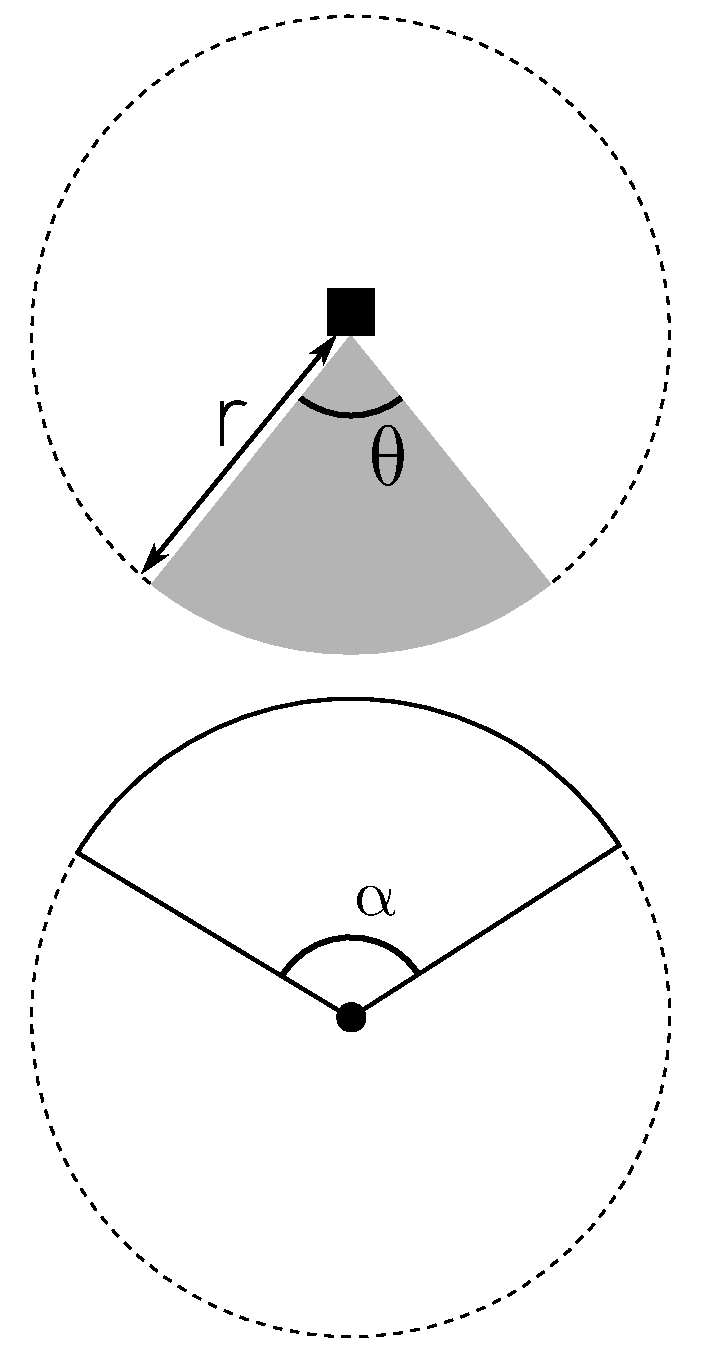
\includegraphics[width=4cm]{imgs/lucas_et_al_figure1.pdf}

\caption[Representation of sensor detection width and animal signal width]{
Representation of sensor detection width and animal signal width.
The filled square and circle represent a sensor and an animal, respectively; $\theta$, sensor detection width (radians); $r$, sensor detection distance; dark grey shaded area, sensor detection zone; $\alpha$, animal signal width (radians).
Dashed lines around the filled square and circle represents the maximum extent of $\theta$ and $\alpha$, respectively.} 
\label{f:AngleDef}
\end{figure}



\subsubsection{Gas Model}

Following \cite{yapp1956theory}, we derive the gas model where sensors can capture animals in any direction and animal signals are detectable from any direction ($\theta =  2\pi$ and $ \alpha =  2\pi$).
We assume that animals are in a homogeneous environment, and move in straight lines of random direction with velocity $v$.
We allow that our stationary sensor can capture animals at a detection distance $r$ and that if an animal moves within this detection zone they are captured with a probability of one; while outside this zone, animals are never captured.

In order to derive animal density, we need to consider relative velocity from the reference frame of the animals.
Conceptually, this requires us to imagine that all animals are stationary and randomly distributed in space, while the sensor moves with velocity $v$.
If we calculate the area covered by the sensor during the survey period, we can estimate the number of animals the sensor should capture.
As a circle moving across a plane, the area covered by the sensor per unit time is $2rv$.
The expected number of captures, $z$, for a survey period of $t$, with an animal density of $D$ is $z = 2rvtD$.
To estimate the density we rearrange to get $D = z/2rvt$.
Note that as $z$ is the number of encounters, not individuals, the possibility of repeated detections of the same individual is accounted for \cite{Hutchinson_Waser_2007}.


\subsubsection{gREM derivations for different detection and signal widths}
Different combinations of $\theta$ and $\alpha$ would be expected to occur (e.g., sensors have different detection widths and animals have different signal widths).
For different combinations $\theta$ and $\alpha$, the area covered per unit time is no longer given by $2rv$.
Instead of the size of the sensor detection zone having a diameter of $2r$, the size changes with the approach angle between the sensor and the animal.
The width of the area within which an animal can be detected is called the profile, $p$.
The size of $p$ depends on the signal width, detector width and the angle that the animal approaches the sensor.
The size of the profile (averaged across all approach angles) is defined as the average profile $\bar{p}$.
However, different combinations of $\theta$ and $\alpha$ need different equations to calculate $\bar{p}$. 




\begin{knitrout}\footnotesize
\definecolor{shadecolor}{rgb}{0.969, 0.969, 0.969}\color{fgcolor}\begin{figure}[t]

{\centering 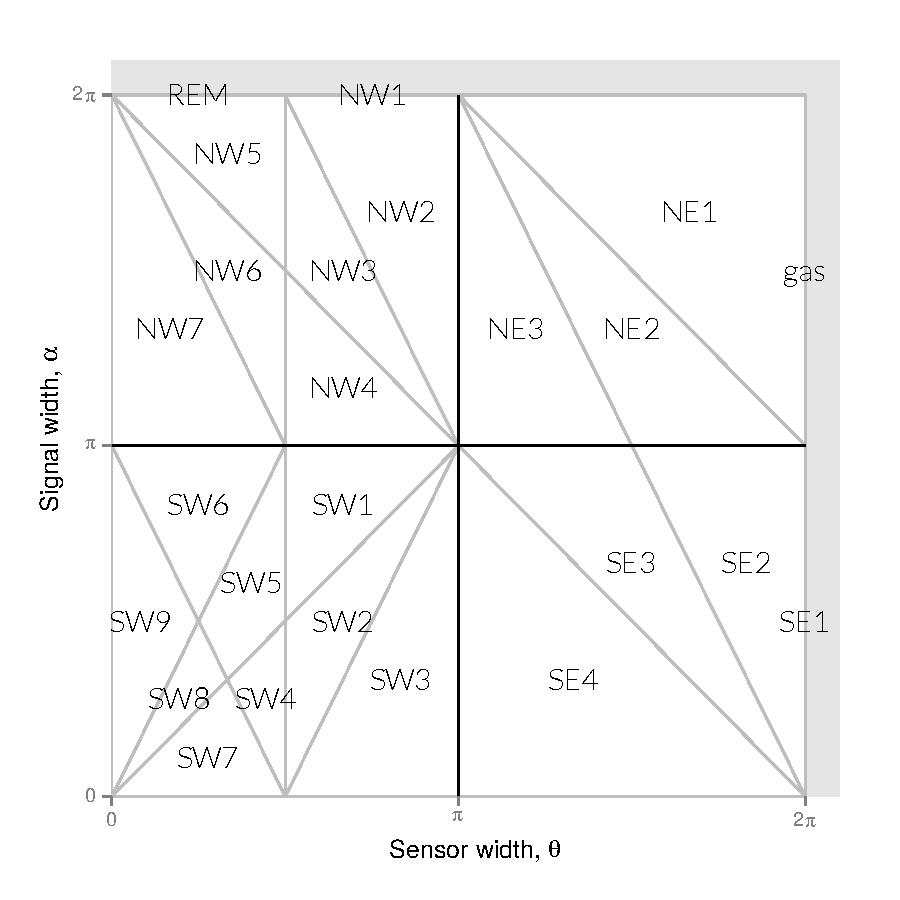
\includegraphics[width=0.6\textwidth]{figure/equalRegions-1} 

}

\caption[Locations where derivation of the average profile $\bar{p}$ is the same]{
Locations where derivation of the average profile $\bar{p}$ is the same for different combinations of sensor detection and animal signal widths.
Symbols within each polygon refer to each gREM submodel named after their compass point, except for Gas and REM which highlight the position of these previously derived models within the gREM.
Symbols on the edge of the plot are for submodels where $\alpha, \theta = 2\pi$
}\label{fig:equalRegions}
\end{figure}


\end{knitrout}

%\begin{figure}
%\centering
%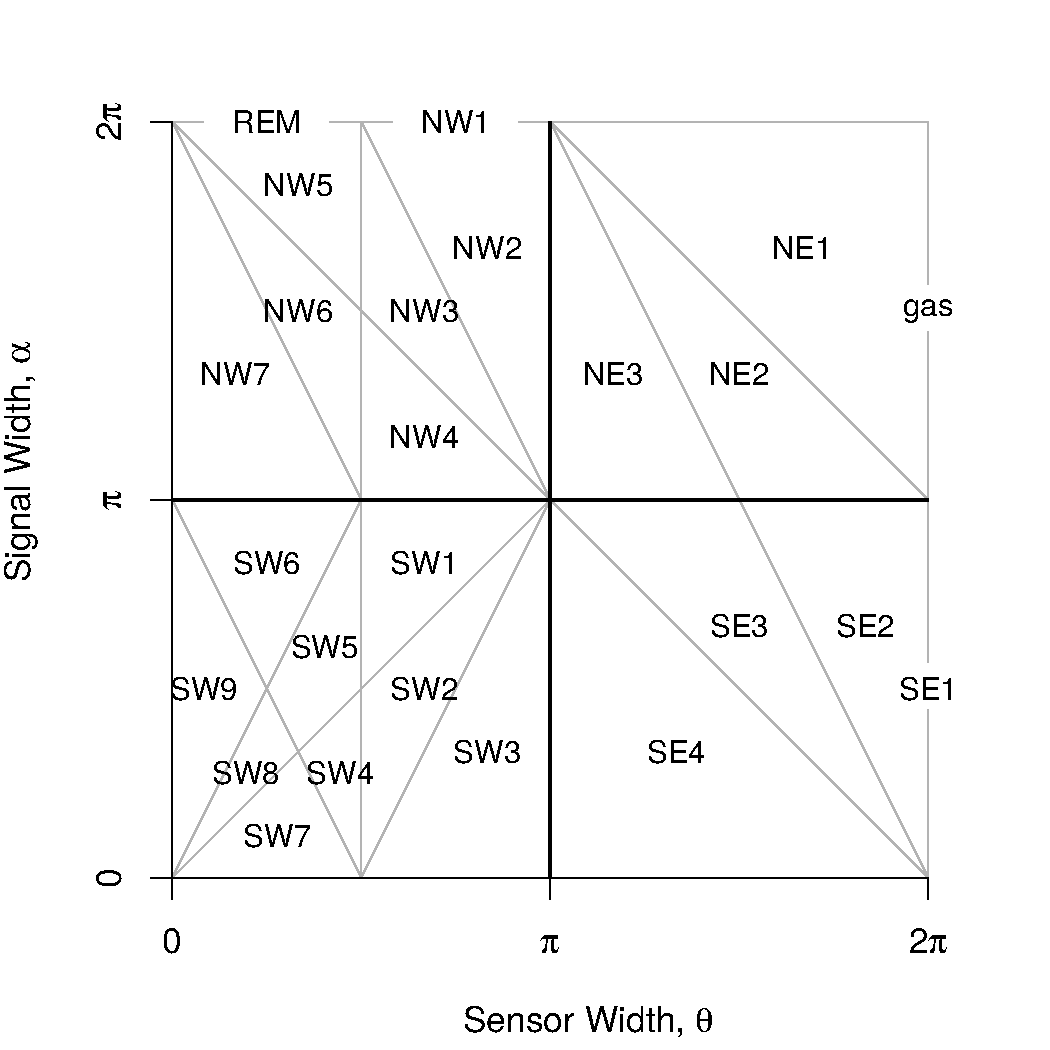
\includegraphics[width=7cm]{imgs/lucas_et_al_figure2.pdf}
%\caption[Locations where derivation of the average profile $\bar{p}$ is the same]{
%Locations where derivation of the average profile $\bar{p}$ is the same for different combinations of sensor detection and animal signal widths.
%Symbols within each polygon refer to each gREM submodel named after their compass point, except for Gas and REM which highlight the position of these previously derived models within the gREM.
%Symbols on the edge of the plot are for submodels where $\alpha, \theta = 2\pi$}
%\label{f:equalRegions}
%\end{figure}

We have identified the parameter space for the combinations of $\theta$ and $\alpha$ for which the derivation of the equations are the same (defined as sub-models in the gREM) (Figure~\ref{fig:equalRegions}).
For example, the gas model becomes the simplest gREM sub-model (upper right in Figure~\ref{fig:equalRegions}) and the REM from \cite{rowcliffe2008estimating} is another gREM sub-model where $\theta<\pi/2$ and $\alpha = 2\pi$.
We derive one gREM sub-model SE2 as an example below, where $2 \pi - \alpha/2 < \theta < 2\pi ,\; 0 < \alpha <\pi$ (see Appendix S2 for derivations of all gREM sub-models).
Any estimate of density would require prior knowledge of animal velocity, $v$ and animal signal width, $\alpha$ taken from other sources, for example existing literature \cite{brinklov2011, carbone2005far}.
Sensor width, $\theta$, and detection distance, $r$ would also need to be measured or obtained from manufacturer specifications \cite{holderied2003echolocation, adams2012you}.


\subsubsection{Example derivation of SE2}

In order to calculate $\bar{p}$, we have to integrate over the focal angle, $x_1$ (Figure~\ref{f:x1AndInt}a).
This is the angle taken from the centre line of the sensor.
Other focal angles are possible ($x_2$, $x_3$, $x_4$) and are used in other gREM sub-models (see Appendix S2).
As the size of the profile depends on the approach angle, we present the derivation across all approach angles.
When the sensor is directly approaching the animal $x_1  = \pi/2$.

Starting from $x_1 = \pi/2$ until $\theta/2 + \pi/2 - \alpha/2$, the size of the profile is $2r\sin \alpha/2$ (Figure~\ref{f:x1AndInt}b).
During this first interval, the size of $\alpha$ limits the width of the profile.
When the animal reaches $x_1$  = $\theta/2 + \pi/2 - \alpha/2$ (Figure~\ref{f:x1AndInt}c), the size of the profile is $r\sin( \alpha/2) + r\cos( x_1  - \theta/2)$ and the size of $\theta$ and $\alpha$ both limit the width of the profile (Figure~ \ref{f:x1AndInt}c).
Finally, at $x_1  = 5\pi/2 - \theta/2  - \alpha/2$ until $x_1  = 3\pi/2$, the width of the profile is again $2r\sin\alpha/2$ (Figure~ \ref{f:x1AndInt}d) and the size of $\alpha$ again limits the width of the profile. 


\begin{figure}[t]
	\centering
	\subfloat[\label{f:intx1}]{
		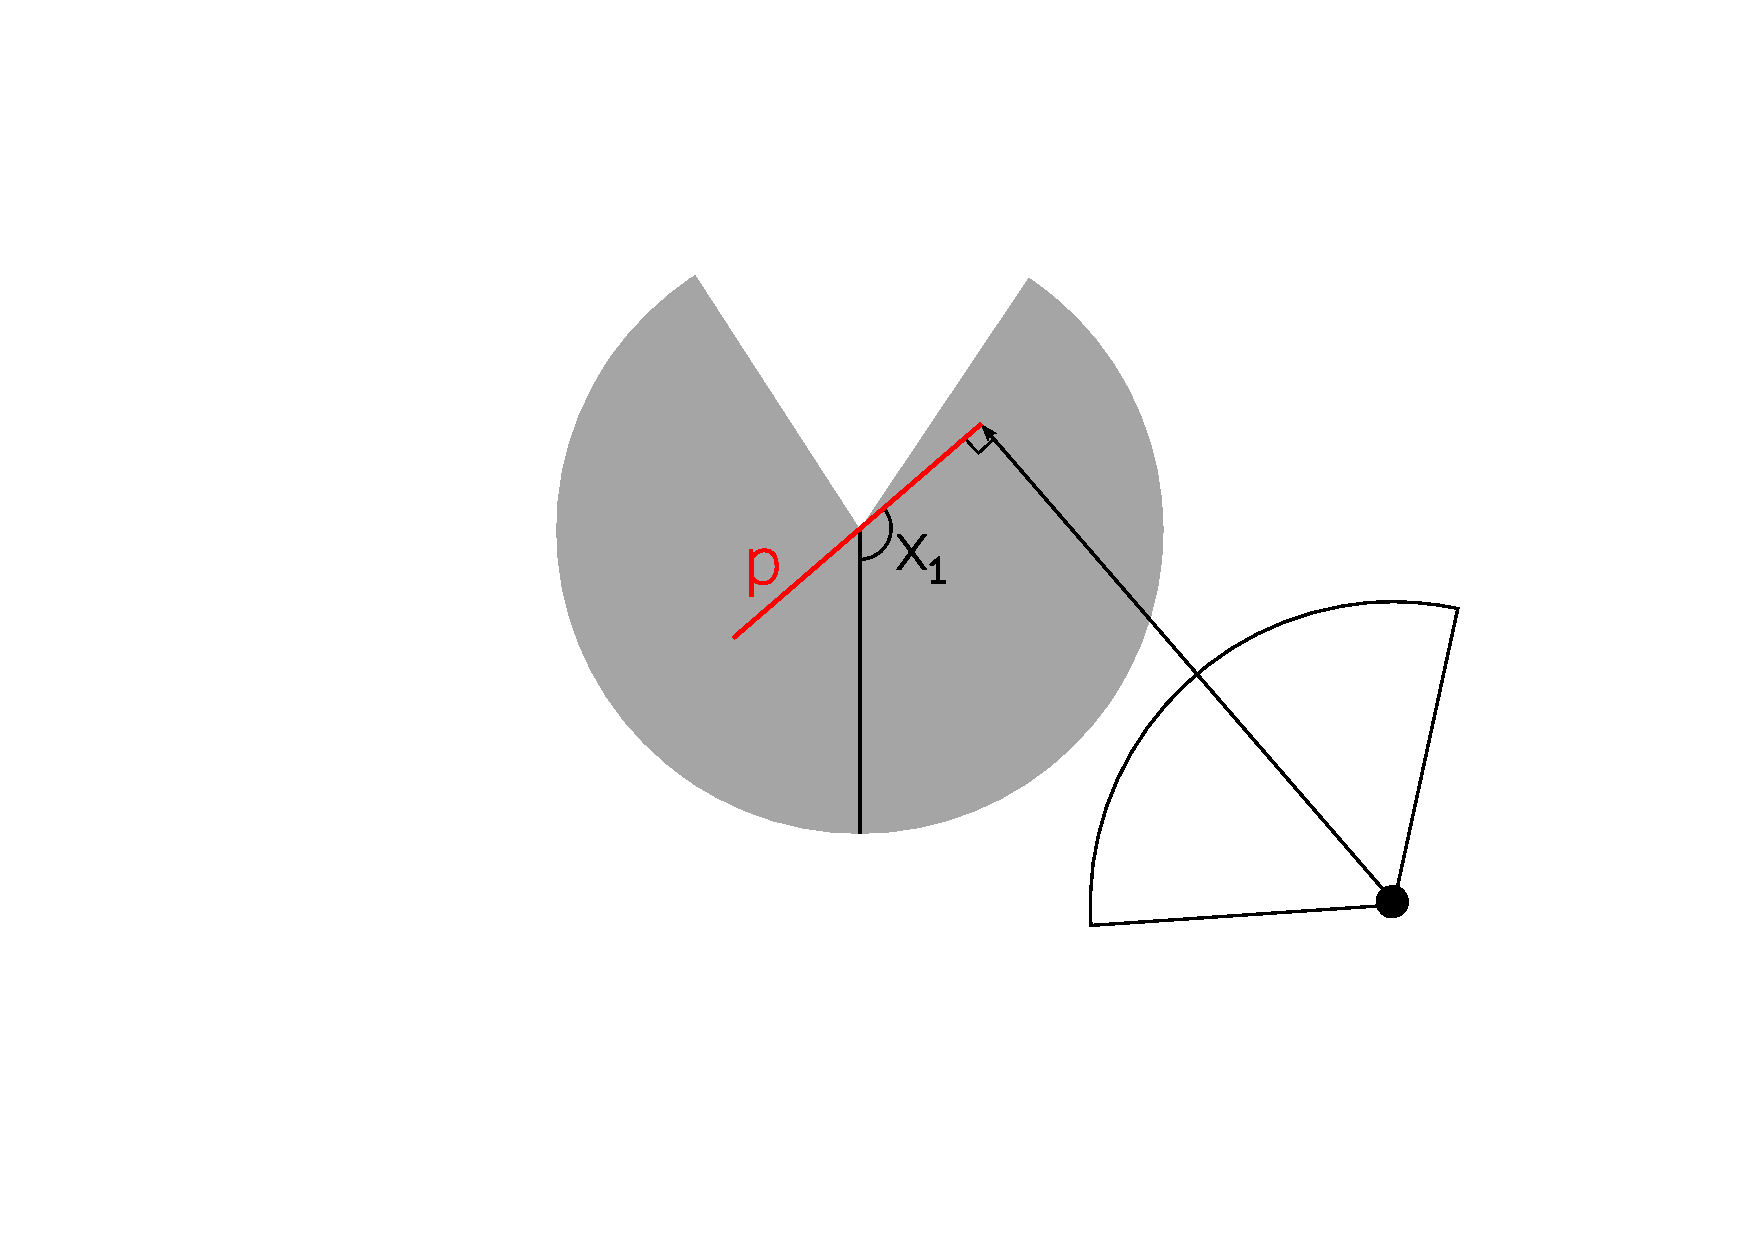
\includegraphics[trim = 20mm 40mm 20mm 10mm, width=70mm]{imgs/x1.pdf}
  }
  \subfloat[\label{f:int1}]{
		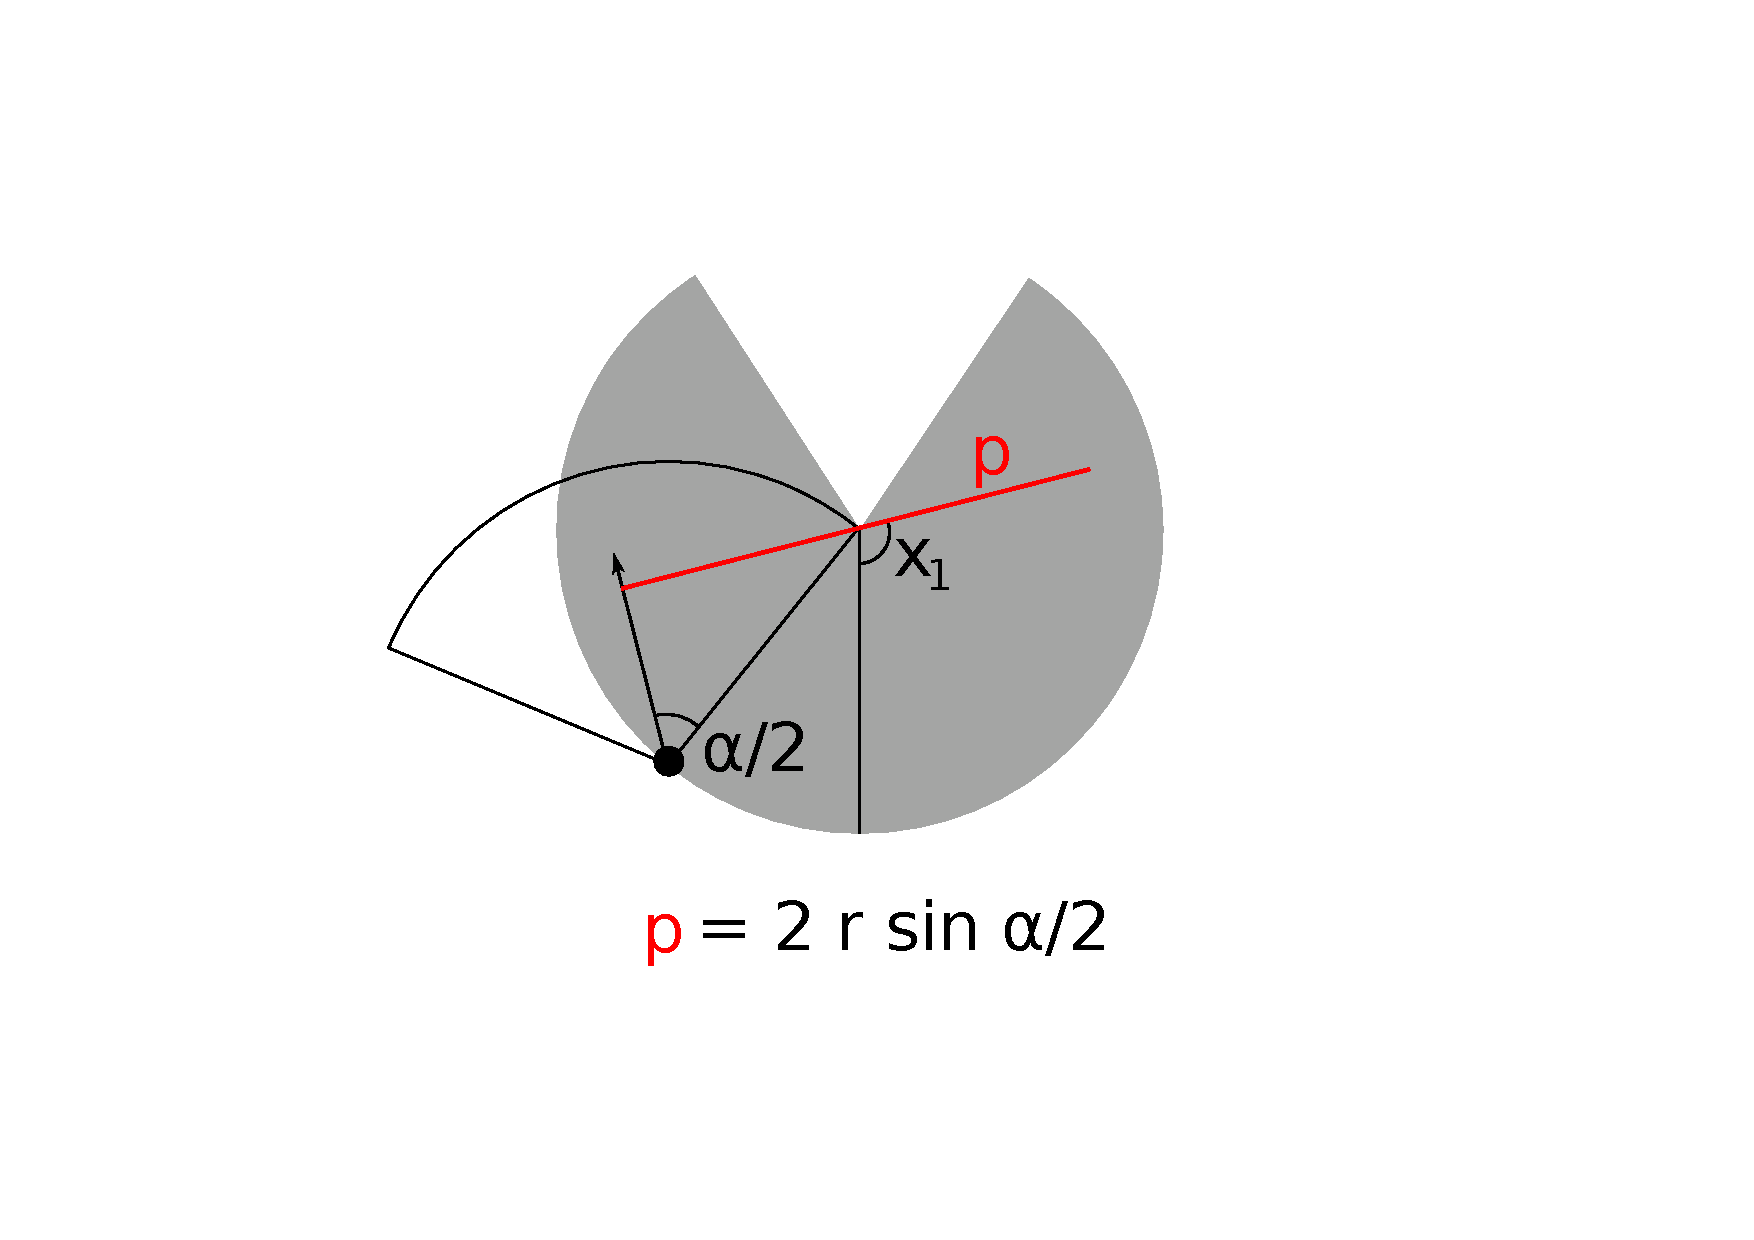
\includegraphics[trim = 20mm 40mm 20mm 10mm, width=70mm]{imgs/firstIntegral.pdf}
  }
  
  \subfloat[\label{f:int2}]{
		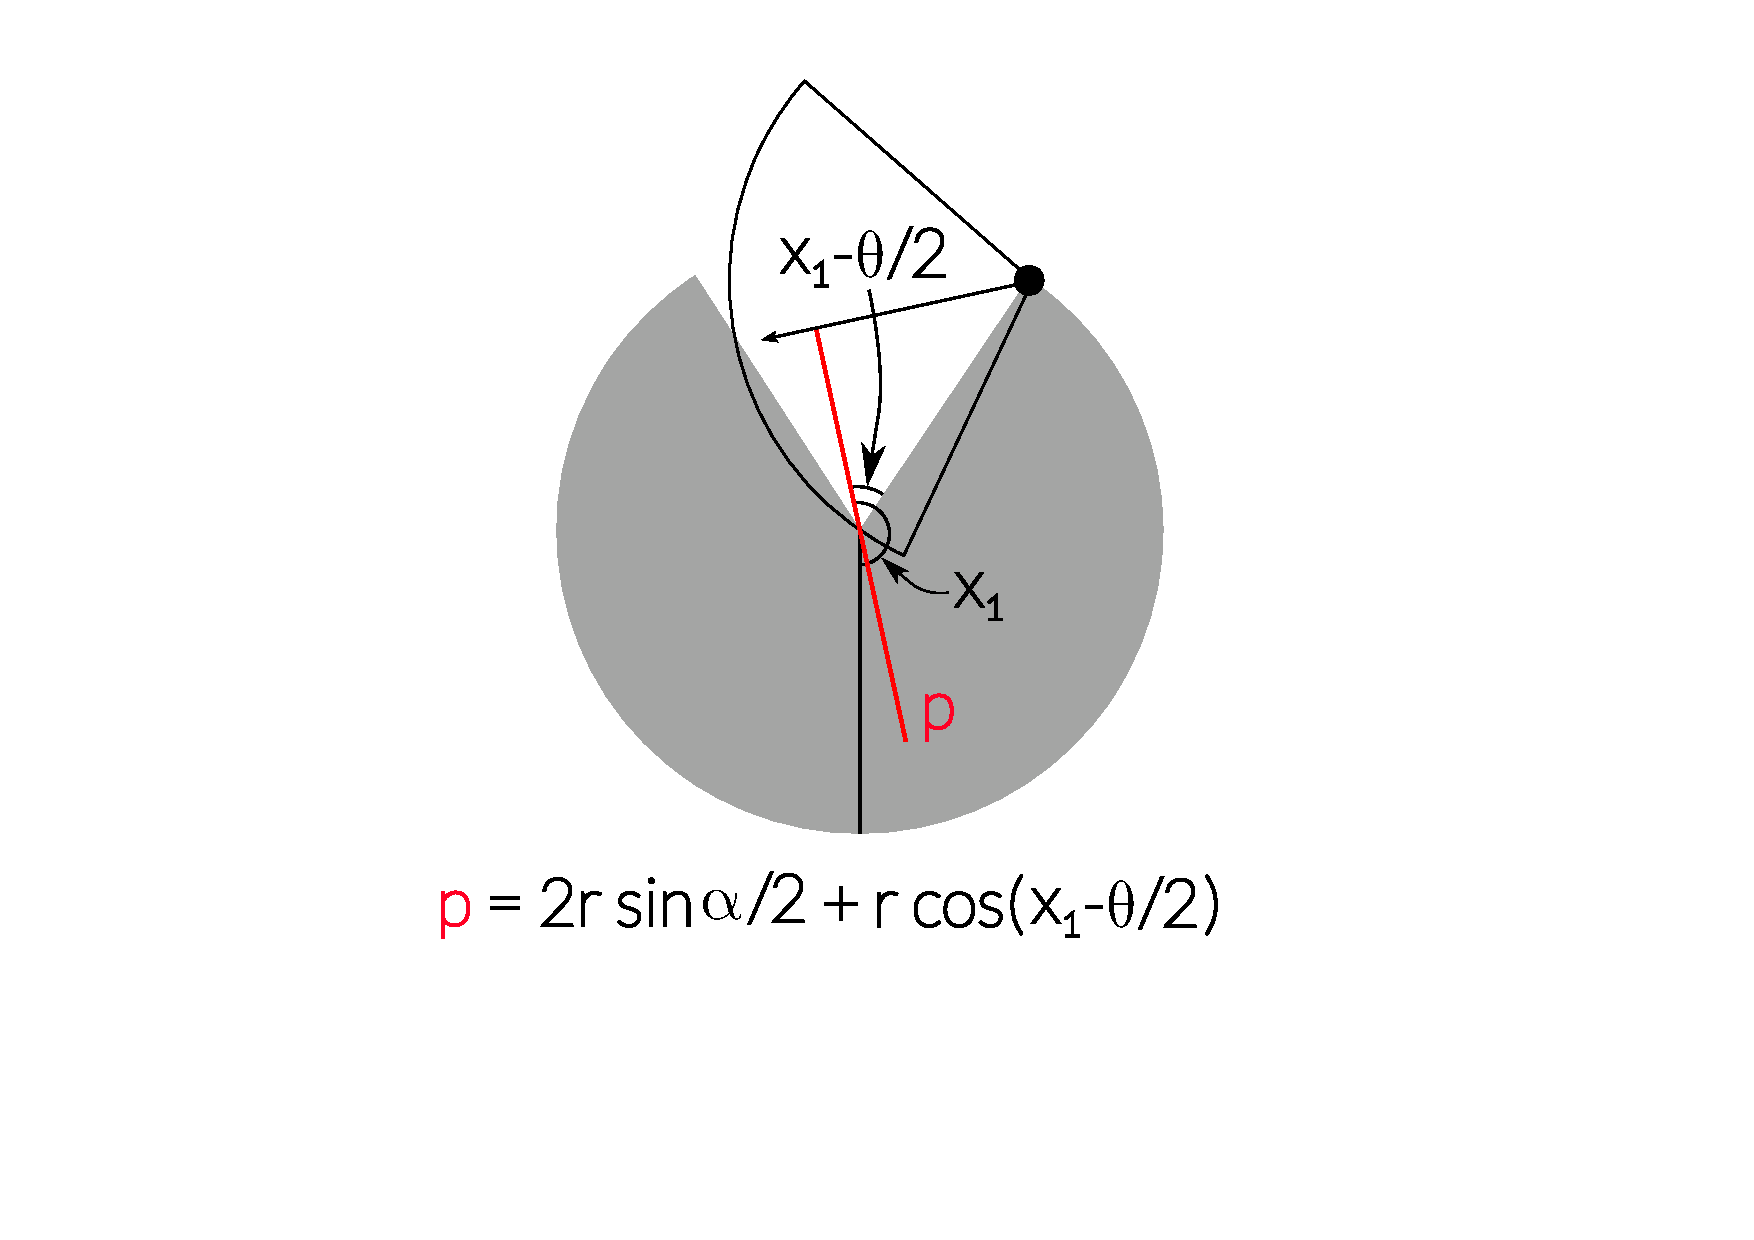
\includegraphics[trim = 20mm 40mm 20mm 10mm, width=70mm]{imgs/secondIntegral.pdf}
  }
  \subfloat[\label{f:int3}]{
		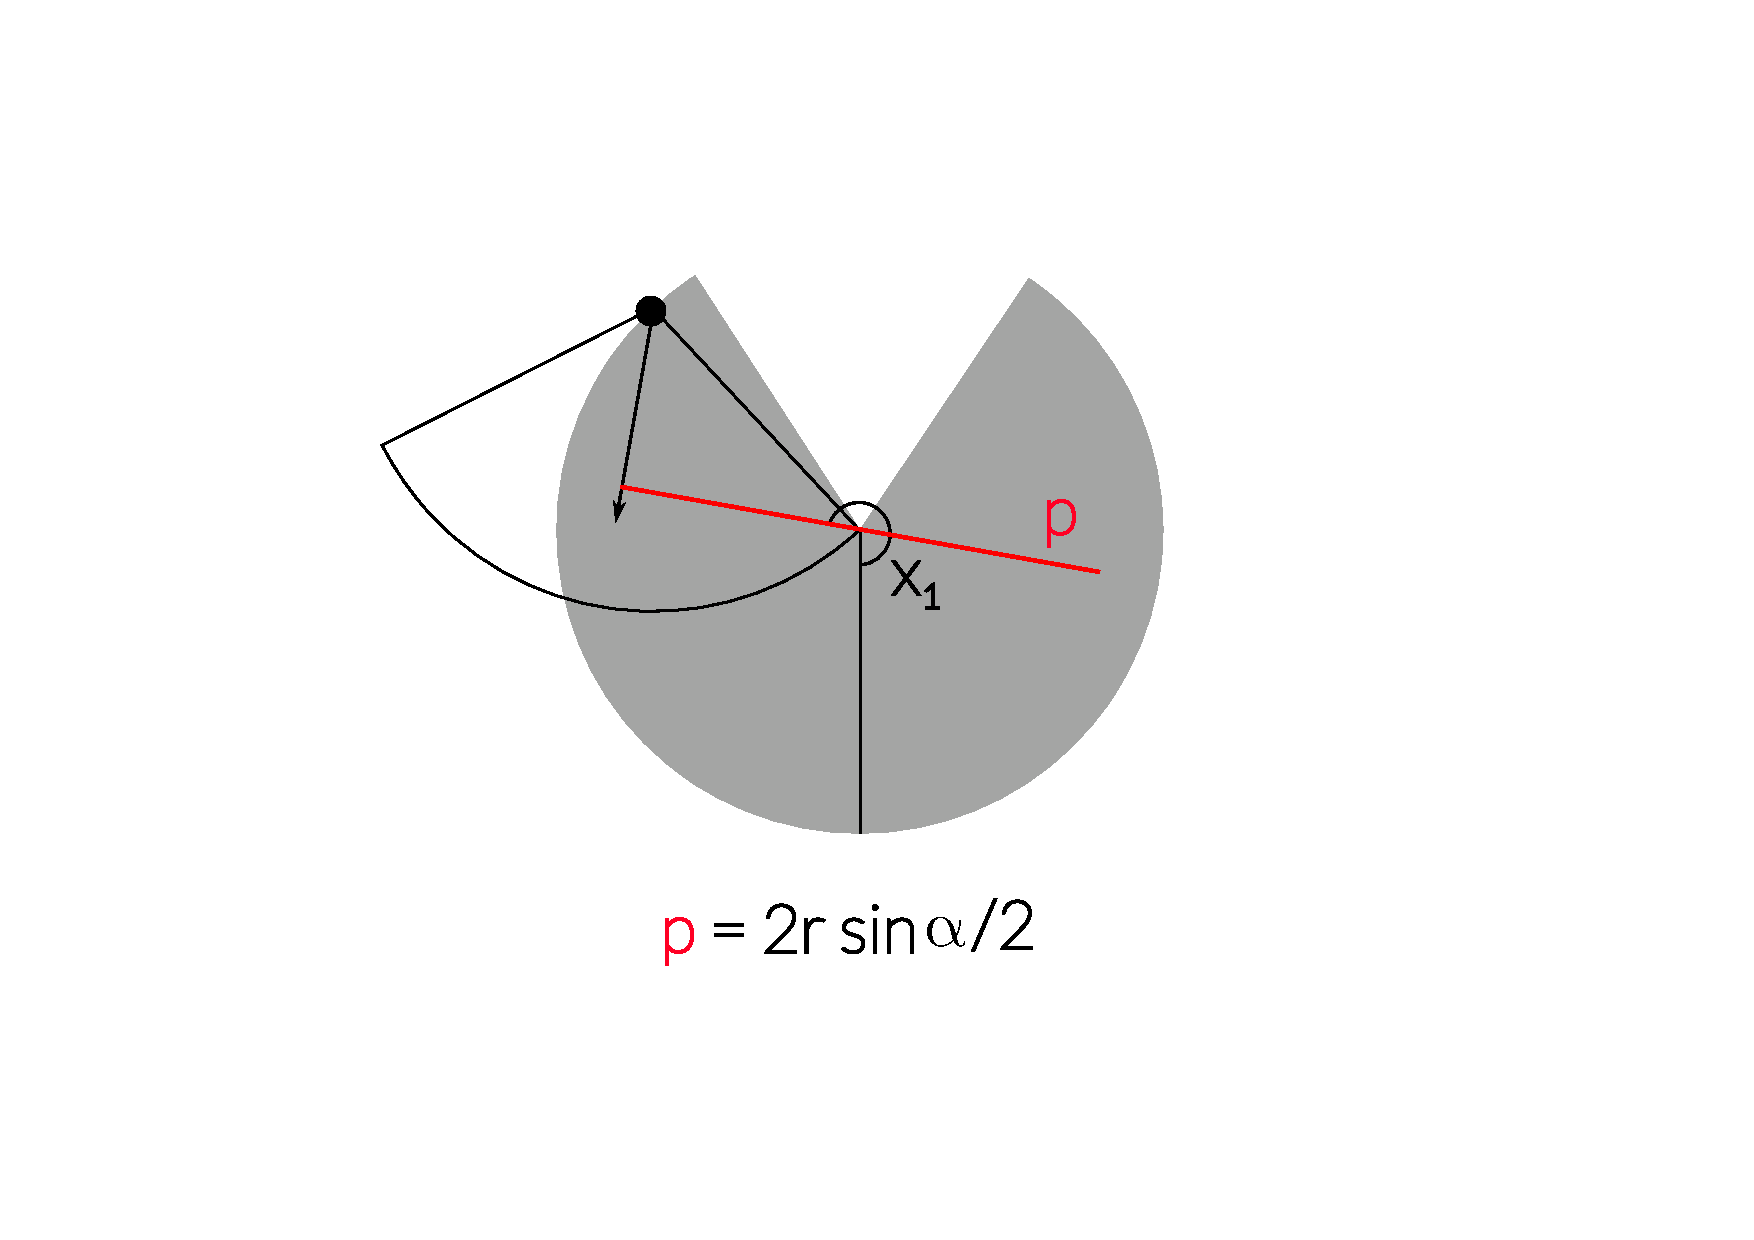
\includegraphics[trim = 20mm 40mm 20mm 10mm, width=70mm]{imgs/thirdIntegral.pdf}
  }

	%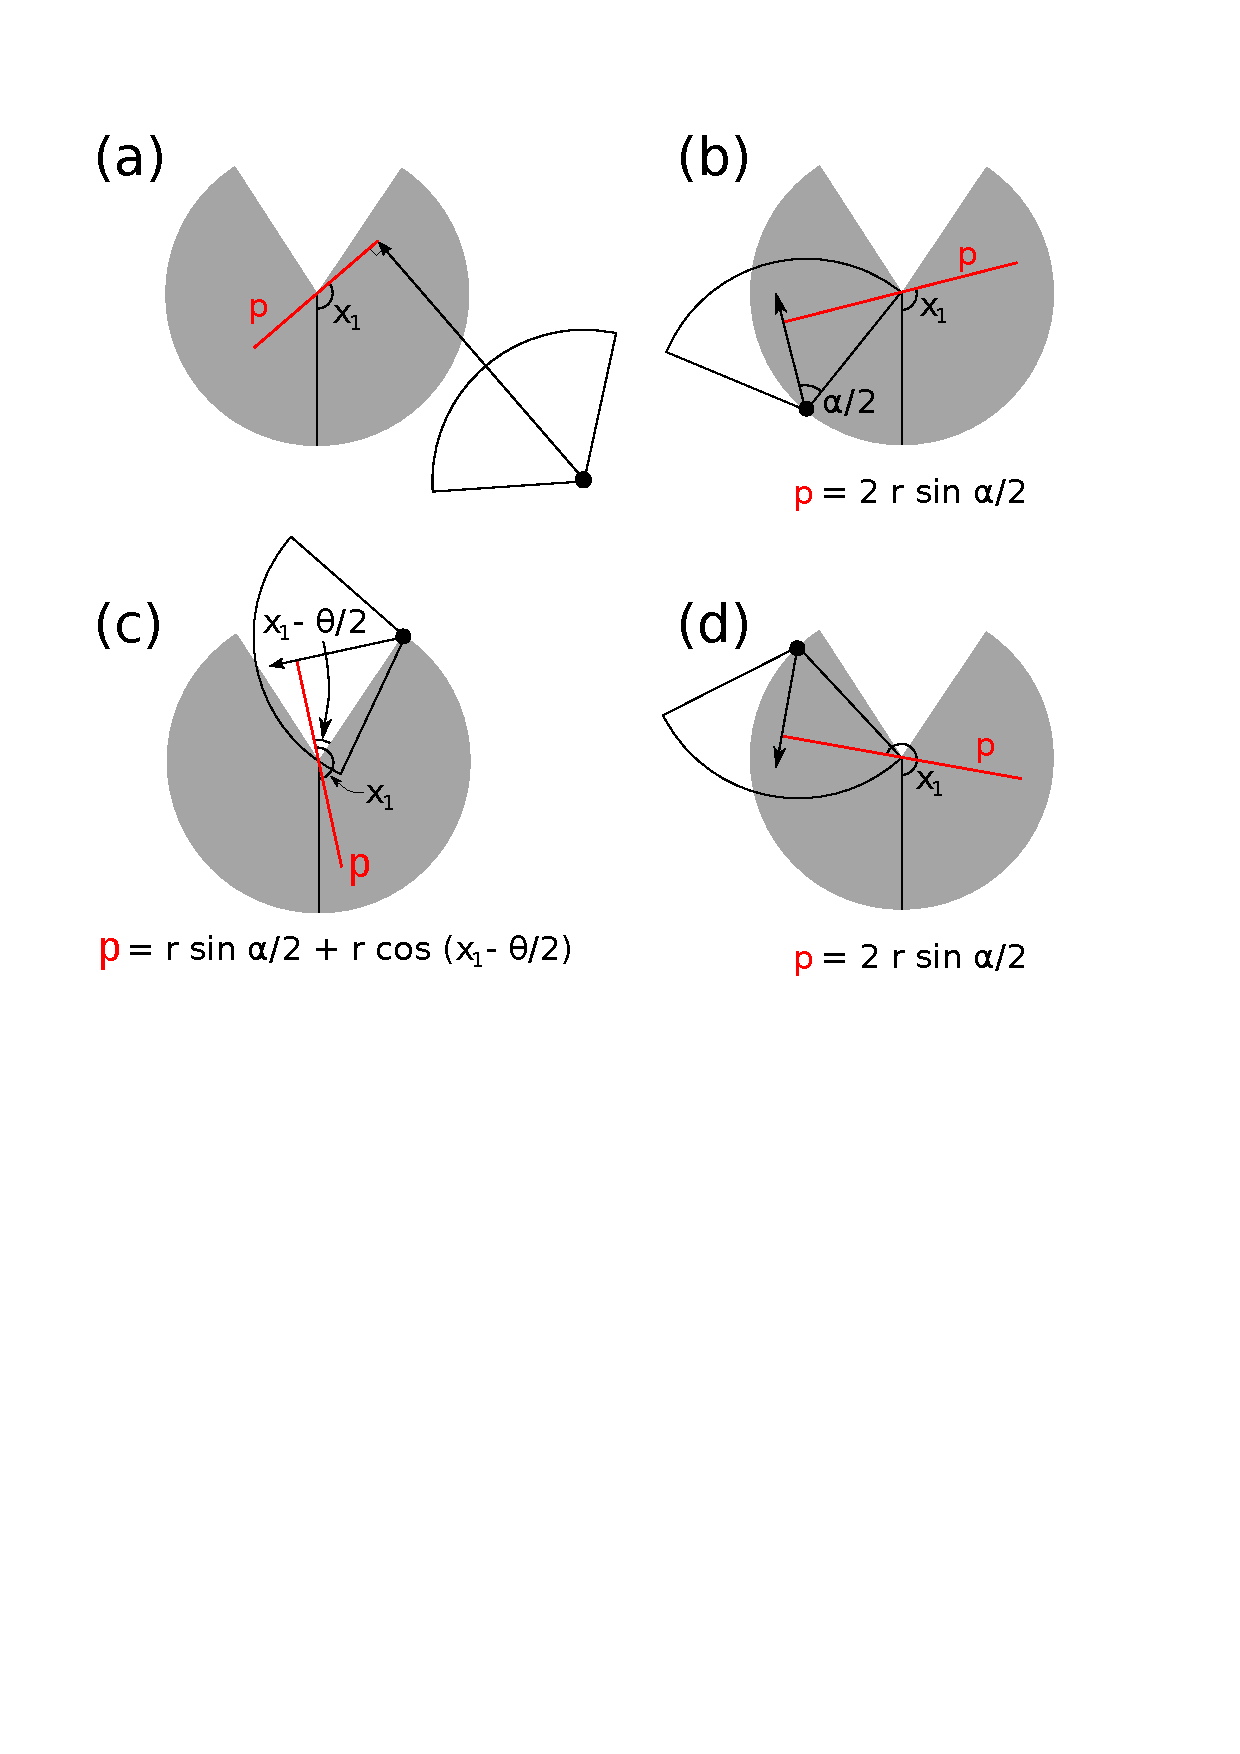
\includegraphics[width=7cm]{imgs/lucas_et_al_figure3.pdf}
\caption[An overview of the derivation of the average profile $\bar{p}$ for the gREM submodel SE2]{
An overview of the derivation of the average profile $\bar{p}$ for the gREM submodel SE2, where (a) shows the location of the profile $p$ (the line an animal must pass through in order to be captured) in red and the focal angle, $x_1$, for an animal (filled circle), its signal (unfilled sector), and direction of movement (shown as an arrow).
The detection zone of the sensor is shown as a filled grey sector with a detection distance of $r$.
The vertical black line within the circle shows the direction the sensor is facing.
The derivation of $p$ changes as the animal approaches the sensor from different directions (shown in b-d), where (b) is the derivation of $p$ when $x_1$ is in the interval $\lbrack\frac{\pi}{2}, \frac{\pi}{2} + \frac{\theta}{2} - \frac{\alpha}{2}\rbrack$, (c)  $p$ when $x_1$ is in the interval $\lbrack\frac{\pi}{2} + \frac{\theta}{2} - \frac{\alpha}{2}, \frac{5 \pi}{2} - \frac{\theta}{2} - \frac{\alpha}{2} \rbrack$ and (d) $p$ when $x_1$ is in the interval $\lbrack\frac{5 \pi}{2} - \frac{\theta}{2} - \frac{\alpha}{2}, \frac{3 \pi}{2}\rbrack$, where $\theta$, sensor detection width; $\alpha$, animal signal width.
The resultant equation for $p$ is shown beneath b-d.
The average profile $\bar{p}$ is the size of the profile averaged across all approach angles.}
\label{f:x1AndInt}

\end{figure}

The profile width $p$ for $\pi$ radians of rotation (from directly towards the sensor to directly behind the sensor) is completely characterised by the three intervals (Figure \ref{f:x1AndInt}b--d).
Average profile width $\bar{p}$ is calculated by integrating these profiles over their appropriate intervals of $x_1$ and dividing by $\pi$ which gives

\begin{align}
    \bar{p} &=\frac{1}{\pi} \left(\int\limits_{\frac{\pi}{2}}^{\frac{\pi}{2} + \frac{\theta}{2} - \frac{\alpha}{2}}2 r \sin{\frac{\alpha}{2} }\;\mathrm{d}x_1+\int\limits_{\frac{\pi}{2} + \frac{\theta}{2} - \frac{\alpha}{2}}^{\frac{5 \pi}{2} - \frac{\theta}{2} - \frac{\alpha}{2}}r \sin{\frac{\alpha}{2} } + r \cos{\left (x_1 - \frac{\theta}{2} \right )}\;\mathrm{d}x_1\right.\notag\\
 &\left.+\int\limits_{\frac{5 \pi}{2} - \frac{\theta}{2} - \frac{\alpha}{2}}^{\frac{3 \pi}{2}}2 r \sin{\frac{\alpha}{2} }\;\mathrm{d}x_1\right) \label{e:SE2int}  \\
     &= \frac{r}{\pi} \left(\theta \sin{\frac{\alpha}{2} } - \cos{\frac{\alpha}{2} } + \cos{\left (\frac{\alpha}{2} + \theta \right )}\right) \label{e:SE2result}
\end{align}

We then use this expression to calculate density
\begin{equation}
\label{e:gas}
D = z/vt\bar{p}.
\end{equation}


Rather than having one equation that describes $\bar{p}$ globally, the gREM must be split into submodels due to discontinuous changes in $p$ as $\alpha$ and $\beta$ change.
These discontinuities can occur for a number of reasons such as a profile switching between being limited by $\alpha$ and $\theta$, the difference between very small profiles and profiles of size zero, and the fact that the width of a sector stops increasing once the central angle reaches $\pi$ radians (i.e., a semi-circle is just as wide as a full circle).
As an example, if $\alpha$ is small, there is an interval between Figure \ref{f:x1AndInt}c and \ref{f:x1AndInt}d where the `blind spot' would prevent animals being detected giving $p=0$.
This would require an extra integral in our equation, as simply putting our small value of $\alpha$ into \ref{e:SE2int} would not give us this integral of $p=0$.

gREM submodel specifications were done by hand, and the integration was done using SymPy \cite{sympy} in Python (Appendix S3).
The gREM submodels were checked by confirming that: (1) submodels adjacent in parameter space were equal at the boundary between them; (2) submodels that border $ \alpha = 0$ had $p = 0$ when $ \alpha = 0$; (3) average profile widths $\bar{p}$ were between 0 and $2r$ and; (4) each integral, divided by the range of angles that it was integrated over, was between 0 and $2r$.
The scripts for these tests are included in Appendix S3 and the R \cite{R} implementation of the gREM is given in Appendix S4.  

\subsection{Simulation Model}

We tested the accuracy and precision of the gREM by developing a spatially explicit simulation of the interaction of sensors and animals using different combinations of sensor detection widths, animal signal widths, number of captures, and models of animal movement.
One hundred simulations were run where each consisted of a  \SI{7.5}{\kilo\meter} by \SI{7.5}{\kilo\meter} square with periodic boundaries.
A stationary sensor of radius $r$, \SI{10}{\meter}, was set up in the exact centre of each simulated study area, covering seven sensor detection widths $\theta$, between 0 and $2\pi$ ($2/9\pi$, $4/9\pi$, $6/9\pi$, $8/9\pi$, $10/9\pi$, $14/9\pi$, and $2\pi$).
Each sensor was set to record continuously and to capture animal signals instantaneously from emission.
Each simulation was populated with a density of \SI{70}{\animals\per\kilo\meter\squared}, calculated from the equation in \cite{damuth1981population} as the expected density of mammals weighing \SI{1}{\gram}.
This density therefore represents a reasonable estimate of density of individuals, given that the smallest mammal is around \SI{2}{\gram} \cite{jones2009pantheria}.
A total of 3937 individuals per simulation were created which were placed randomly at the start of the simulation. 11 signal widths $\alpha$ between 0 and $\pi$ were used ($1/11\pi$, $2/11\pi$, $3/11\pi$, $4/11\pi$, $5/11\pi$, $6/11\pi$, $7/11\pi$, $8/11\pi$, $9/11\pi$, $10/11\pi$, $\pi$). 

Each simulation lasted for $N$ steps (14400) of duration $T$ (15 minutes) giving a total duration of 150 days.
The individuals moved within each step with a distance $d$, with an average speed, $v$.
The distance, $d$, was sampled from a normal distribution with mean distance, $\mu_d = vT$, and standard deviation, $\sigma_d = vT/10$, where the standard deviation was chosen to scale with the average distance travelled.
An average speed, $v = $ \SI{40}{\kilo\meter \per \day}, was chosen based on the largest day range of terrestrial animals \cite{carbone2005far}, and represents the upper limit of realistic speeds.
At the end of each step, individuals were allowed to either remain stationary for a time step (with a given probability, $S$), or change direction where the change in direction has a uniform distribution in the interval $\left[-A, A\right]$.
This resulted in seven different movement models where: (1) simple movement, where $S$ and $A$ = 0; (2) stop-start movement, where (i) $S$ = 0.25, $A$ = 0, (ii) $S$ = 0.5, $A$ = 0, (iii) $S$ = 0.75, $A$ = 0; (3) correlated random walk movement, where (i) $S$ = 0, $A$ = $\pi/3$, (ii) $S$ = 0, $A$ = $2\pi/3$, iii) $S$ = 0, $A$ = $\pi$.
Individuals were counted as they moved into the detection zone of the sensor per simulation. 

We calculated the estimated animal density from the gREM by summing the number of captures per simulation and inputting these values into the correct gREM submodel.
The accuracy of the gREM was determined by comparing the true simulation density with the estimated density.
Precision of the gREM was determined by the standard deviation of estimated densities.
We used this method to compare the accuracy and precision of all the gREM submodels.
As these submodels are derived for different combinations of $\alpha$ and $\theta$, the accuracy and precision of the submodels was used to determine the impact of different values of $\alpha$ and $\theta$. 

The influence of the number of captures and animal movement models on accuracy and precision was investigated using four different gREM submodels representative of the range $\alpha$ and $\theta$ values (submodels NW1, SW1, NE1, and SE3, Figure~\ref{fig:equalRegions}).
From a random starting point we ran the simulation until a range of different capture numbers were recorded (from 10 to 100 captures), recorded the length of time this took, and estimated the animal density for each of the four sub-models.
These estimated densities were compared to the true density to assess the impact on the accuracy and precision of the gREM.
We calculated the coefficient of variation in order to compare the precision of the density estimates from simulations with different expected numbers of captures.
The gREM also assumes that individuals move continuously with straight-line movement (simple movement model) and we therefore assessed the impact of breaking the gREM assumptions.
We used the four submodels to compare the accuracy and precision of a simple movement model, stop-start movement models (using different average amounts of time spent stationary), and random walk movement models.
Finally, as the parameters ($\alpha$, $\beta$, $r$ and $v$) are likely to be measured with error, we compared true simulation densities to densities estimated with parameters with errors of $0\%$, $\pm 5\%$ and $\pm 10\%$, for all gREM submodels.


\section{Results}

\subsection{Analytical model}

The equation for $\bar{p}$ has been newly derived for each submodel in the gREM, except for the gas model and REM which have been calculated previously.
However, many models, although derived separately, have the same expression for $\bar{p}$.
Figure~\ref{f:equalModelResults} shows the expression for $\bar{p}$ in each case.
The general equation for density, \ref{e:gas}, is used with the correct value of $\bar{p}$ substituted.
Although more thorough checks are performed in Appendix S3, it can be seen that all adjacent expressions in Figure~\ref{f:equalModelResults} are equal when expressions for the boundaries between them are substituted in.






\begin{figure}
	\centering
	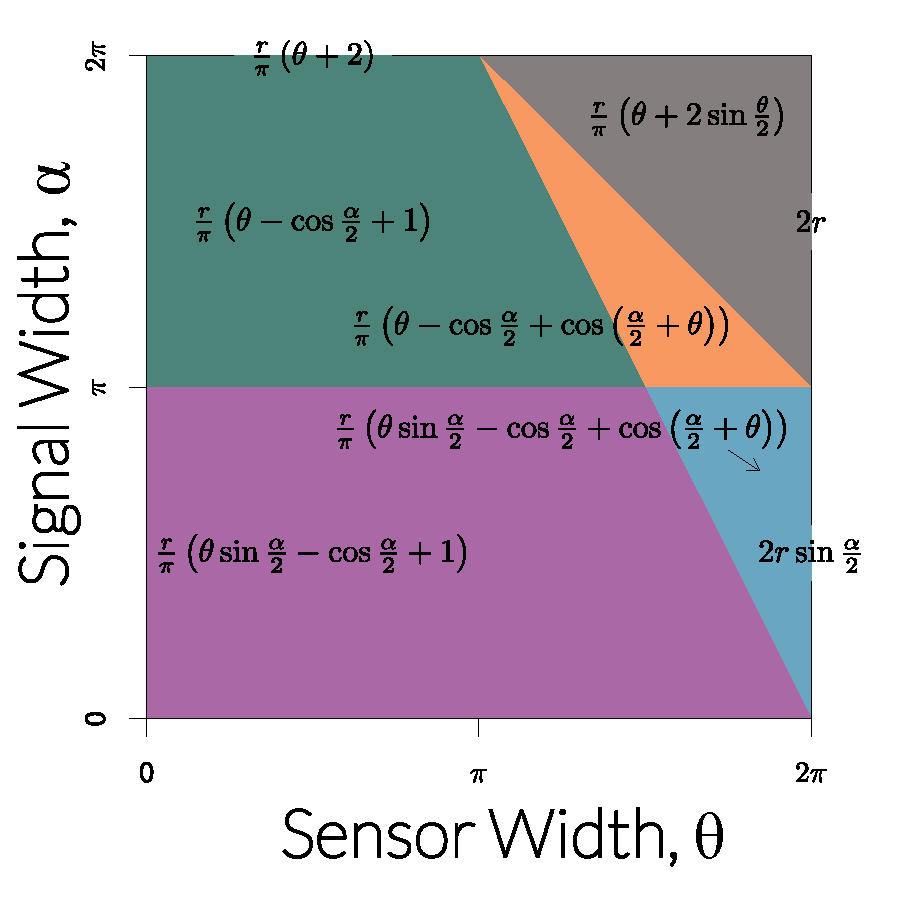
\includegraphics[width=7cm]{imgs/equalRegionsExpressions.pdf}
	\caption[Expressions for the average profile width]{
Expressions for the average profile width, $\bar{p}$, given a range of sensor and signal widths.
Despite independent derivation within each block, many models result in the same expression.
These are collected together and presented as one block of colour.
Expressions on the edge of the plot are for submodels with $\alpha, \theta = 2\pi$. }
	\label{f:equalModelResults}
\end{figure}


\subsection{Simulation model}

\subsubsection{gREM submodels}
All gREM submodels showed a high accuracy, i.e., the median difference between the estimated and true values was less than 2\% across all models (Figure~\ref{fig:gremSubmods}).
However, the precision of the submodels do vary, where the gas model is the most precise and the SW7 sub model the least precise, having the smallest and the largest interquartile range, respectively (Figure~\ref{fig:gremSubmods}).
The standard deviation of the error between the estimated and true densities is strongly related to both the sensor and signal widths (Appendix S5), such that larger widths have lower standard deviations (greater precision) due to the increased capture rate of these models.



\begin{knitrout}\footnotesize
\definecolor{shadecolor}{rgb}{0.969, 0.969, 0.969}\color{fgcolor}\begin{figure}[t]

{\centering 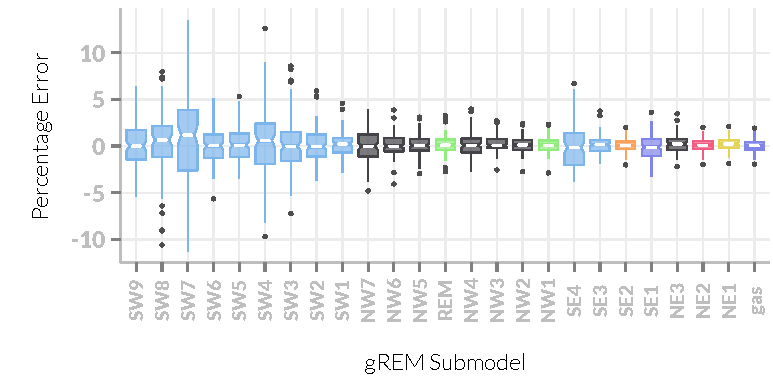
\includegraphics[width=\textwidth]{figure/gremSubmods-1} 

}

\caption[Simulation model results of the accuracy and precision for gREM submodels]{
Simulation model results of the accuracy and precision for gREM submodels.
The percentage error between estimated and true density for each gREM sub model is shown within each box plot, where the white line represents the median percentage error across all simulations, boxes represent the middle 50\% of the data, whiskers represent variability outside the upper and lower quartiles with outliers plotted as individual points.
Notches indicate 95\% confidence intervals.
Box colours correspond to the expressions for average profile width $\bar{p}$ given in Figure \ref{f:equalModelResults}. 
}\label{fig:gremSubmods}
\end{figure}


\end{knitrout}

%\begin{figure}[t]
%	\centering
%	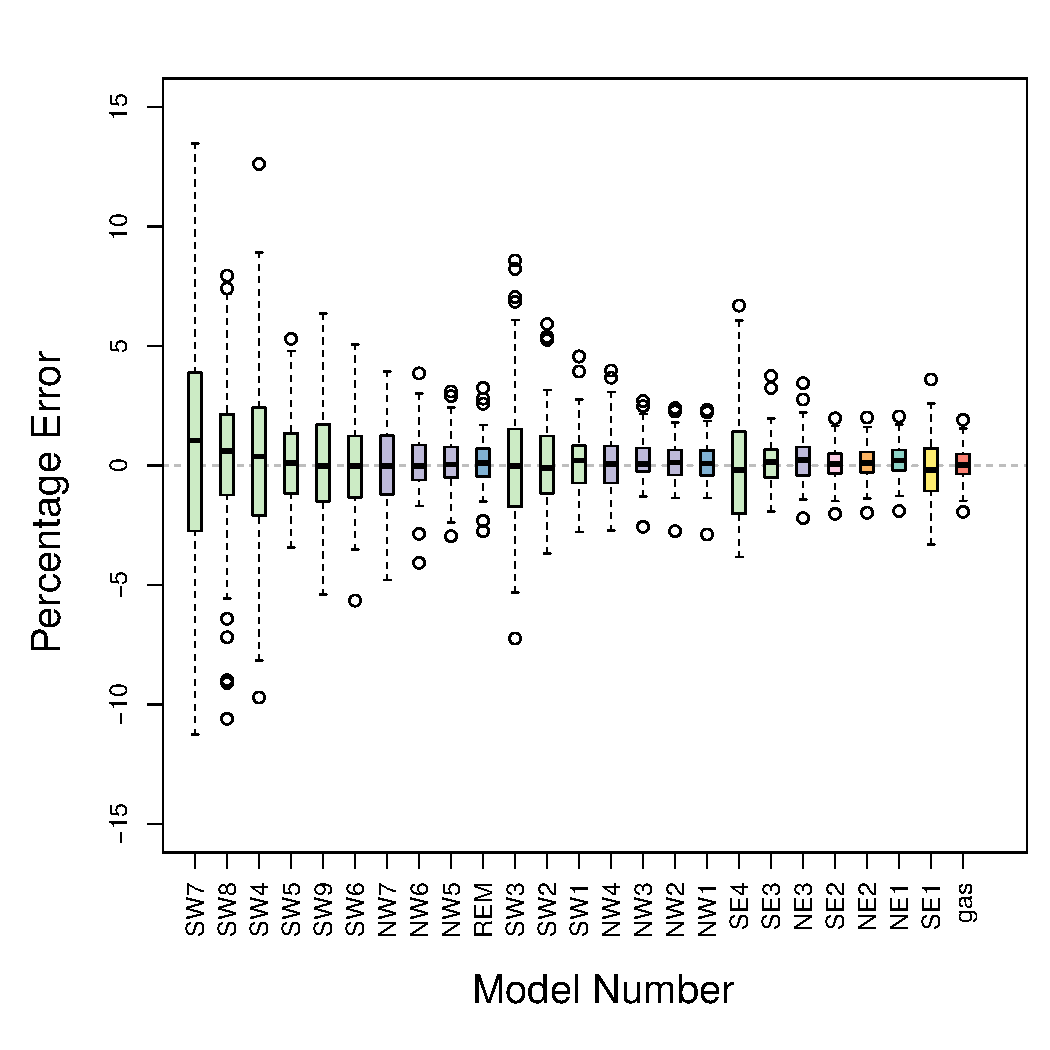
\includegraphics[width=7cm]{imgs/lucas_et_al_figure5.pdf}
%       	\caption[Simulation model results of the accuracy and precision for gREM submodels]{Simulation model results of the accuracy and precision for gREM submodels.
%The percentage error between estimated and true density for each gREM sub model is shown within each box plot, where the black line represents the median percentage error across all simulations, boxes represent the middle 50\% of the data, whiskers represent variability outside the upper and lower quartiles with outliers plotted as individual points.
%Box colours correspond to the expressions for average profile width $\bar{p}$ given in Figure 4.        
%} 
%	\label{f:ModelBias}
%\end{figure}

\subsubsection{Number of captures}

Within the four gREM submodels tested (NW1, SW1, SE3, NE1), the accuracy was not strongly affected by the number of captures.
The median difference between the estimated and true values was less than 15\% across all capture rates (Figure~\ref{fig:Captures}).
However, the precision was dependent on the number of captures across all four of the gREM submodels, where precision increases as number of captures increases, as would be expected for any statistical estimate (Figure~\ref{fig:Captures}).
For all gREM submodels, the the coefficient of variation falls to 10\% at 100 captures. 



\begin{knitrout}\footnotesize
\definecolor{shadecolor}{rgb}{0.969, 0.969, 0.969}\color{fgcolor}\begin{figure}[t]

{\centering 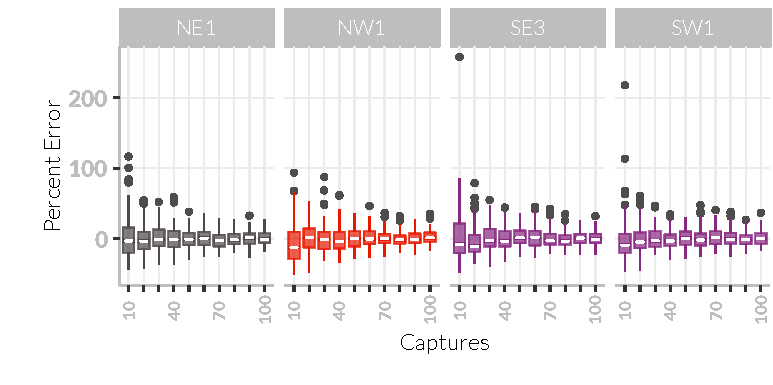
\includegraphics[width=0.8\textwidth]{figure/Captures-1} 

}

\caption[Simulation model results of the accuracy and precision of four gREM submodels]{
Simulation model results of the accuracy and precision of four gREM submodels (NW1, SW1, SE3 and NE1) given different numbers of captures.
The percentage error between estimated and true density within each gREM sub model for capture rate is shown within each box plot, where the white line represents the median percentage error across all simulations, boxes represent the middle 50\% of the data, whiskers represent variability outside the upper and lower quartiles with outliers plotted as individual points.
Notches show the 95\% confidence interval.
Sensor and signal widths vary between submodels.
The numbers beneath each plot represent the coefficient of variation.
The colour of each box plot corresponds to the expressions for average profile width $\bar{p}$ given in Figure \ref{f:equalModelResults}. 
}\label{fig:Captures}
\end{figure}


\end{knitrout}

%\begin{figure}[t]
%  \centering
%	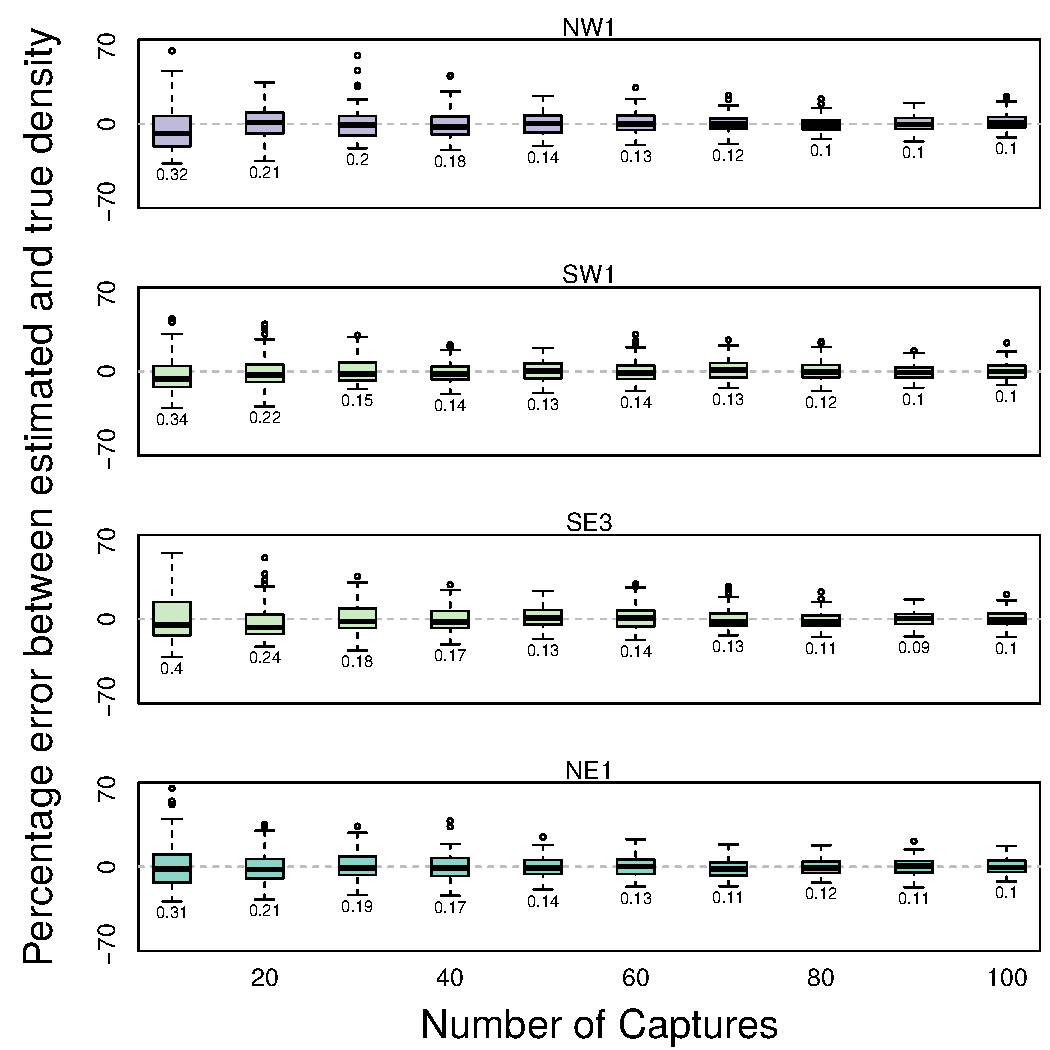
\includegraphics[width=7cm]{imgs/lucas_et_al_figure6.pdf}
%\caption[Simulation model results of the accuracy and precision of four gREM submodels]{
%Simulation model results of the accuracy and precision of four gREM submodels (NW1, SW1, SE3 and NE1) given different numbers of captures.
%The percentage error between estimated and true density within each gREM sub model for capture rate is shown within each box plot, where the black line represents the median percentage error across all simulations, boxes represent the middle 50\% of the data, whiskers represent variability outside the upper and lower quartiles with outliers plotted as individual points.
%Sensor and signal widths vary between submodels.
%The numbers beneath each plot represent the coefficient of variation.
%The colour of each box plot corresponds to the expressions for average profile width $\bar{p}$ given in Figure 4. }            
%\label{f:Captures}
%\end{figure}

\subsubsection{Movement models}

Within the four gREM submodels tested (NW1, SW1, SE3, NE1), neither the accuracy or precision was affected by the average amount of time spent stationary.
The median difference between the estimated and true values was less than 2\% for each category of stationary time (0, 0.25, 0.5 and 0.75) (Figure~\ref{fig:movtFig}).
Altering the maximum change in direction in each step (0, $\pi/3$, $2\pi/3$, and $\pi$) did not affect the accuracy or precision of the four gREM submodels (Figure~\ref{fig:movtFig}). 

\subsubsection{Impact of parameter error}

The percentage error in the density estimates across all parameters and gREM submodels shows a similar response for under and over estimated parameters, suggesting the accuracy is reasonable with respect to parameter error (Appendix S6).
The impact of parameter error on the precision of the density estimate varies across gREM submodels and parameters, where $\alpha$ shows the largest variation including the largest values.
However, in all cases the percentage error in the density estimate is not more than 5\% greater than the error in the parameter estimate (Appendix S6).



\begin{knitrout}\footnotesize
\definecolor{shadecolor}{rgb}{0.969, 0.969, 0.969}\color{fgcolor}\begin{figure}[t]

{\centering 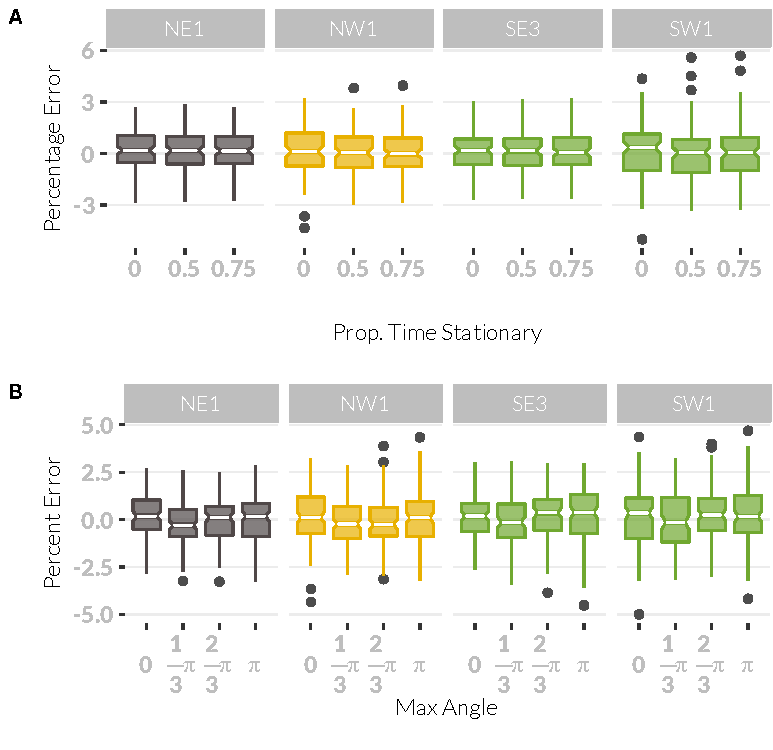
\includegraphics[width=0.7\textwidth]{figure/movtFig-1} 

}

\caption[Simulation model results of the accuracy and precision of four gREM submodels]{
Simulation model results of the accuracy and precision of four gREM submodels (NW1, SW1, SE3 and NE1) given different movement models where (a) average amount of time spent stationary (stop-start movement) and (b) maximum change in direction at each step (correlated random walk model).
The percentage error between estimated and true density within each gREM sub model for the different movement models is shown within each box plot, where the white line represents the median percentage error across all simulations, boxes represent the middle 50\% of the data, whiskers represent variability outside the upper and lower quartiles with outliers plotted as individual points.
Notches in boxplots show the 95\% confidence for the median.
The simple model is represented where time and maximum change in direction equals 0.
The colour of each box plot corresponds to the expressions for average profile width $\bar{p}$ given in Figure 4.
}\label{fig:movtFig}
\end{figure}


\end{knitrout}

                  
%%%% ------- Discussion ---------%%%%
\section{Discussion}

\subsection{Analytical model}

We have developed the gREM such that it can be used to estimate density from acoustic sensors and camera traps.
This has entailed a generalisation of the gas model and the REM in \cite{rowcliffe2008estimating} to be applicable to any combination of sensor width  $\theta$ and signal directionality $\alpha$.
We emphasise that the approach is robust to multiple detections of the same individual.
We have used simulations to show, as a proof of principle, that these models are accurate and precise. 

There are a number of possible extensions to the gREM which could be developed in the future.
The original gas model was formulated for the case where both animals and sensor are moving \cite{Hutchinson_Waser_2007}.
Indeed any of the models which have animals that are equally detectable in all directions ($\alpha = 2\pi$) can be trivially expanded by replacing animal speed $v$ with $v + v_s$ where $v_s$ is the speed of the sensor.
However, when the animal has a directional call the extension becomes less simple.
The approach would be to calculate again the mean profile width.
However, for each angle of approach, one would have to average the profile width for an animal facing in any direction (i.e., not necessarily moving towards the sensor) weighted by the relative velocity of that direction.
There are a number of situations where a moving detector and animal could occur, e.g.
an acoustic detector towed from a boat when studying porpoises \cite{kimura2014acoustic} or surveying echolocating bats from a moving car \cite{jones2011indicator}. 

Interesting but unstudied problems impacting the gREM are firstly, edge effects caused by sensor trigger delays (the delay between sensing an animal and attempting to record the encounter) \cite{rovero2013camera}, and secondly, sensors which repeatedly turn on an off during sampling \cite{jones2011indicator}.
The second problem is particularly relevant to acoustic detectors which record ultrasound by time expansion.
Here ultrasound is recorded for a set time period and then slowed down and played back, rendering the sensor 'deaf' periodically during sampling.
Both of these problems may cause biases in the gREM, as animals can move through the detection zone without being detected.
As the gREM assumes constant surveillance, the error created by switching the sensor on and off quickly will become more important if the sensor is only on for short periods of time.
We recommend that the gREM is applied to constantly sampled data, and the impacts of breaking these assumptions on the gREM should be further explored. 

\subsection{Accuracy, Precision and Recommendations for Best Practice}
Based on our simulations, we believe that the gREM has the potential to produce accurate estimates for many different species, using either camera traps or acoustic detectors.
However, the precision of the gREM differed between submodels.
For example, when the sensor and signal width were small, the precision of the model was reduced.
Therefore when choosing a sensor for use in a gREM study, the sensor detection width should be maximised.
If the study species has a narrow signal directionality, other aspects of the study protocol, such as length of the survey, should be used to compensate. 

The precision of the gREM is greatly affected by the number of captures.
The coefficient of variation falls dramatically between 10 and 60 captures and then after this continues to slowly reduce.
At 100 captures the submodels reach 10\% coefficient of variation, considered to be a very good level of precision and better than many previous studies \cite{thomas2012passive, o2003crouching, foster2012critique}.  The length of surveys in the field will need to be adjusted so that enough data can be collected to reach this precision level.
Populations of fast moving animals or populations with high densities will require less survey effort than those species that are slow moving or have populations with low densities. 

We found that the sensitivity of the gREM to inaccurate parameter estimates was both predictable and reasonable (Appendix S6), although this varies between different parameters and gREM submodels.
Whilst care should be taken in parameter estimation when analysing both acoustic and camera trap data, acoustic data poses particular problems.
For acoustic surveys, estimates of $r$ (detection distance) can be measured directly or calculated using sound attenuation models \cite{holderied2003echolocation}, while the sensor angle is often easily measured \cite{adams2012you} or found in the manufacturer's specifications.
When estimating animal movement speed $v$, only the speed of movement during the survey period should be used.
The signal width is the most sensitive parameter to inaccurate estimates (Appendix S6) and is also the most difficult to measure.  While this parameter will typically be assumed to be $2\pi$ for camera trap surveys, fewer estimates exist for acoustic signal widths.
Although signal width has been measured for echolocating bats using arrays of microphones \cite{brinklov2011}, more work should be done on obtaining estimates for a range of acoustically surveyed species.



\subsection{Limitations}

Although the REM has been found to be effective in field tests \cite{rowcliffe2008estimating, zero2013monitoring}, the gREM requires further validation by both field tests and simulations.
For example, capture-mark-recapture methods could be used alongside the gREM to test the accuracy under field conditions \cite{rowcliffe2008estimating}.
While we found no effect of the movement model on the accuracy or precision of the gREM, the models we have used in our simulations to validate the gREM are still simple representations of true animal movement.
Animal movement may be highly nonlinear and often dependent on multiple factors such as behavioural state and existence of home ranges \cite{smouse2010stochastic}.
Therefore testing the gREM against real animal data, or further simulations with more complex movement models, would be beneficial.

The assumptions of our simulations may require further consideration, for example we have assumed an equal density across the study area.
However, in a field environment the situation may be more complex, with additional variation coming from local changes in density between sensor sites.
Athough unequal densities should theoretically not affect accuracy \cite{Hutchinson_Waser_2007}, it will affect precision and further simulations should be used to quantify this effect.
Additionally, we allowed the sensor to be stationary and continuously detecting, negating the triggering, and non-continuous recording issues that could exist with some sensors and reduce precision or accuracy.
Finally, in the simulation animals moved at the equivalent of the largest day range of terrestrial animals \cite{carbone2005far}.
Slower speed values should not alter the accuracy of the gREM, but precision would be affected since slower speeds produce fewer records.
The gREM was both accurate and precise for all the movement models we tested (stop-start movement and correlated random walks).

A feature of the gREM is that it does not fit a statistical model to estimate detection probability as occupancy models and distance sampling do \cite{royle2003estimating, barlow2005estimates, marques2011estimating}.
Instead it explicitly models the process, with animals only being detected if they approach the sensor from a suitable direction.
Other processes that affect detection probability could be included in the model to improve realism.

\subsection{Implications for ecology and conservation}

The gREM is applicable for count data obtained either visually or acoustically in both marine and terrestrial environments, and is suitable for taxa including echolocating bats \cite{walters2012continental}, songbirds \cite{buckland2006point}, whales \cite{marques2011estimating} and forest primates \cite{hassel2008reliable}.
Many of these taxa contain critically endangered species and monitoring their populations is of conservation interest.
For example, current methods of density estimation for the threatened Franciscana dolphin (\emph{Pontoporia blainvillei}) may result in underestimation of their numbers \cite{crespo2010abundance}.
In addition, using gREM may be easier than other methods for measuring the density of animals which may be useful in quantifying ecosystem services, such as songbirds with a known positive influence on pest control \cite{jirinec2011roosting}.

The gREM will aid researchers to study species with non-invasive methods such as remote sensors, which allows for large, continuous monitoring projects with limited human resources \cite{kelly2012noninvasive}.
The gREM is also suitable  for species that are sensitive to human contact or are difficult or dangerous to catch \cite{thomas2012passive}.
As sensors such as camera traps and acoustic detectors become more ubiquitous, the gREM will be increasingly useful for monitoring unmarked animal populations across broad spatial, temporal and taxonomic scales.


%%%% ------- Acknowledgments ---------%%%%
%\section{Acknowledgments}
%We thank Hilde Wilkinson-Herbot, Chris Carbone, Francois Balloux, Andrew Cunningham, Steve Hailes, Richard Glennie and an anonymous referee for comments on previous versions of the manuscript.
%This study was funded through CoMPLEX PhD studentships at University College London supported by BBSRC and EPSRC (EAM and TCDL) and The Darwin Initiative (Awards 15003, 161333, EIDPR075), NERC (NE/H525003/1), and The Leverhulme Trust (Philip Leverhulme Prize) for KEJ.

%%%% ------- Data Accessibility ---------%%%%
%\section{Data Accessibility}

%The code used in this chapter is available on Github at \url{https://github.com/timcdlucas/lucasMoorcroftManuscript/tree/postPeerReview}.




\chapter{General Conclusions}
\label{chapterlabel4}

\lettr{M}y conclusions.
% This just dumps some pseudolatin in so you can see some text in place.
\blindtext




\addcontentsline{toc}{chapter}{Appendices}




% The \appendix command resets the chapter counter, and changes the chapter numbering scheme to capital letters.
%\chapter{Appendices}
\appendix

% I switched the order so chapter 2 \includes chapter3
\chapter{Appendix: A comparative test of the role of population structure in determining pathogen richness}
\chaptermark{Appendix: A comparative test of population structure and pathogen richness}
\label{empirAppendix}











%%-------------------------------------------------------------------------------%%
%% Give full data tables for both analyses.
%%-------------------------------------------------------------------------------%%










\begin{landscape}

% latex table generated in R 3.2.4 by xtable 1.8-2 package
% Thu Apr 14 16:07:10 2016
\begingroup\tiny
\begin{longtable}{@{}llrrrrrrrrrr@{}}
\caption{Raw species for both number of subspecies analyses} \\ 
  \toprule
Family & Binomial & Virus Sp. & Subspecies & Gene Flow & Mass & Range Size & Scholar & PubMed & Range Width & Dmax & Reference \\ 
  &  &  &  &  & (g) & ($\times 10^{9}$km$^2$) &  &  & (km) & (km) &  \\ 
   \midrule\endhead 
Megadermatidae & \emph{Macroderma gigas} & 0 &  & 0.25 & 124.37 & 1078.95 & 769 & 13 & 3609.23 & 3148 & \cite{wilmer1999genetic} \\ 
  Miniopteridae & \emph{Miniopterus natalensis} & 0 &  & 0.08 & 10.43 & 3784.83 & 180 & 5 & 6657.28 & 1706 & \cite{miller2003strong} \\ 
  Miniopteridae & \emph{Miniopterus schreibersii} & 12 &  & 1.86 & 11.46 & 3707.97 & 3090 & 64 & 7050.77 & 2649 & \cite{witsenburg2015haemosporidian} \\ 
  Phyllostomidae & \emph{Macrotus waterhousii} & 0 &  & 2.33 & 16.27 & 802.74 & 594 & 15 & 4298.38 & 935 & \cite{burns2014correlates} \\ 
  Pteropodidae & \emph{Rousettus obliviosus} & 0 &  & 13.76 & 45.32 & 1.67 & 52 & 0 & 174.92 & 160 & \cite{goodman2010phylogeny} \\ 
  Pteropodidae & \emph{Thoopterus nigrescens} & 0 &  & 0.14 & 66.12 & 182.87 & 52 & 0 & 1388.27 & 620 & \cite{burns2014correlates} \\ 
  Vespertilionidae & \emph{Myotis ciliolabrum} & 0 &  & 12.38 & 4.89 & 1388.27 & 592 & 5 & 2150.93 & 473 & \cite{burns2014correlates} \\ 
  Vespertilionidae & \emph{Myotis macropus} & 0 &  & 0.44 & 9.8 & 1326.85 & 214 & 0 & 3644.70 & 883 & \cite{burns2014correlates} \\ 
  Hipposideridae & \emph{Hipposideros speoris} & 2 & 1 & 0.07 & 10.39 & 1225.28 & 603 & 9 & 2801.74 & 1175 & \cite{chinnasamy2013genetic} \\ 
  Phyllostomidae & \emph{Desmodus rotundus} & 7 & 1 & 1.29 & 33.16 & 17726.52 & 6810 & 265 & 9314.10 & 2252 & \cite{burns2014correlates} \\ 
  Phyllostomidae & \emph{Macrotus californicus} & 1 & 1 & 1.26 & 11.83 & 643.20 & 808 & 15 & 2139.83 & 590 & \cite{burns2014correlates} \\ 
  Pteropodidae & \emph{Cynopterus sphinx} & 3 & 6 & 5.08 & 44.71 & 6456.51 & 1620 & 53 & 6821.48 & 3915 & \cite{burns2014correlates} \\ 
  Pteropodidae & \emph{Pteropus alecto} & 6 & 4 & 5.31 & 610.13 & 1354.21 & 1530 & 49 & 5064.99 & 2961 & \cite{webb1996mobility} \\ 
  Pteropodidae & \emph{Pteropus conspicillatus} & 2 & 2 & 2.92 & 760.71 & 219.53 & 465 & 15 & 3294.68 & 993 & \cite{fox2006population} \\ 
  Pteropodidae & \emph{Pteropus poliocephalus} & 3 & 1 & 8.80 & 702.78 & 249.32 & 1950 & 54 & 1844.19 & 721 & \cite{webb1996mobility} \\ 
  Pteropodidae & \emph{Pteropus scapulatus} & 7 & 1 & 4.34 & 380.35 & 3038.11 & 707 & 19 & 4053.21 & 2625 & \cite{burns2014correlates} \\ 
  Pteropodidae & \emph{Rousettus leschenaultii} & 11 & 3 & 17.73 & 84.88 & 6764.79 & 848 & 0 & 6795.10 & 3828 & \cite{burns2014correlates} \\ 
  Pteropodidae & \emph{Rousettus madagascariensis} & 1 & 1 & 31.12 & 65.72 & 292.74 & 135 & 2 & 1483.04 & 1366 & \cite{burns2014correlates} \\ 
  Rhinolophidae & \emph{Rhinolophus ferrumequinum} & 9 & 7 & 2.78 & 22.59 & 9747.14 & 5070 & 85 & 12178.06 & 9670 & \cite{burns2014correlates} \\ 
  Vespertilionidae & \emph{Lasiurus borealis} & 1 & 1 & 19.61 & 12.33 & 4881.50 & 3460 & 28 & 4185.94 & 2198 & \cite{vonhofgenetic} \\ 
  Vespertilionidae & \emph{Myotis lucifugus} & 8 & 5 & 7.64 & 7.8 & 12040.88 & 9720 & 298 & 6671.21 & 5173 & \cite{vonhof2015range} \\ 
  Vespertilionidae & \emph{Myotis myotis} & 6 & 2 & 3.45 & 25.59 & 3874.58 & 8880 & 137 & 4377.75 & 2786 & \cite{burns2014correlates} \\ 
  Vespertilionidae & \emph{Myotis ricketti} & 3 & 1 & 2.38 & 22.5 & 987.18 & 421 & 11 & 2741.15 & 2272.57 & \cite{lu2013phylogeography} \\ 
  Vespertilionidae & \emph{Nyctalus noctula} & 8 & 4 & 20.71 & 28.48 & 8033.97 & 4670 & 37 & 10238.26 & 4015 & \cite{burns2014correlates} \\ 
  Emballonuridae & \emph{Rhynchonycteris naso} & 1 & 1 &  & 4.14 & 11508.83 & 607 & 2 &  &  &  \\ 
  Emballonuridae & \emph{Saccolaimus flaviventris} & 1 & 1 &  & 45.25 & 6053.68 & 342 & 3 &  &  &  \\ 
  Emballonuridae & \emph{Taphozous melanopogon} & 4 & 5 &  & 25.99 & 5624.37 & 503 & 15 &  &  &  \\ 
  Emballonuridae & \emph{Taphozous perforatus} & 2 & 4 &  & 24.43 & 2114.92 & 264 & 5 &  &  &  \\ 
  Hipposideridae & \emph{Aselliscus stoliczkanus} & 1 & 1 &  & 6.09 & 1362.32 & 128 & 9 &  &  &  \\ 
  Hipposideridae & \emph{Hipposideros armiger} & 5 & 4 &  & 49.99 & 4475.41 & 656 & 26 &  &  &  \\ 
  Hipposideridae & \emph{Hipposideros bicolor} & 1 & 7 &  & 8.39 & 1584.43 & 371 & 4 &  &  &  \\ 
  Hipposideridae & \emph{Hipposideros caffer} & 3 & 4 &  & 9.46 & 6348.39 & 458 & 6 &  &  &  \\ 
  Hipposideridae & \emph{Hipposideros cineraceus} & 1 & 2 &  & 3.84 & 2203.63 & 164 & 0 &  &  &  \\ 
  Hipposideridae & \emph{Hipposideros commersoni} & 1 & 1 &  & 89.99 & 513.16 & 429 & 0 &  &  &  \\ 
  Hipposideridae & \emph{Hipposideros diadema} & 2 & 15 &  & 46.9 & 3318.84 & 472 & 4 &  &  &  \\ 
  Hipposideridae & \emph{Hipposideros lankadiva} & 1 & 1 &  & 44.76 & 712.59 & 188 & 2 &  &  &  \\ 
  Hipposideridae & \emph{Hipposideros larvatus} & 2 & 5 &  & 19.95 & 3287.88 & 398 & 7 &  &  &  \\ 
  Hipposideridae & \emph{Hipposideros pomona} & 2 & 3 &  & 6.2 & 2840.90 & 226 & 5 &  &  &  \\ 
  Megadermatidae & \emph{Megaderma lyra} & 2 & 2 &  & 39.27 & 6042.09 & 1370 & 32 &  &  &  \\ 
  Molossidae & \emph{Chaerephon plicatus} & 2 & 5 &  & 21.83 & 2462.34 & 62 & 0 &  &  &  \\ 
  Molossidae & \emph{Chaerephon pumilus} & 4 & 1 &  & 10.98 & 7240.27 & 177 & 0 &  &  &  \\ 
  Molossidae & \emph{Cynomops abrasus} & 1 & 4 &  & 35.39 & 10671.17 & 143 & 2 &  &  &  \\ 
  Molossidae & \emph{Cynomops planirostris} & 1 & 1 &  & 12.84 & 11450.26 & 138 & 0 &  &  &  \\ 
  Molossidae & \emph{Eumops auripendulus} & 1 & 2 &  & 28.49 & 14106.77 & 343 & 2 &  &  &  \\ 
  Molossidae & \emph{Eumops glaucinus} & 1 & 2 &  & 36.2 & 11385.12 & 545 & 5 &  &  &  \\ 
  Molossidae & \emph{Eumops perotis} & 1 & 3 &  & 50.97 & 11695.63 & 859 & 5 &  &  &  \\ 
  Molossidae & \emph{Molossops neglectus} & 1 & 1 &  & 11 & 6515.61 & 166 & 0 &  &  &  \\ 
  Molossidae & \emph{Molossus molossus} & 7 & 7 &  & 13.7 & 15767.72 & 2220 & 68 &  &  &  \\ 
  Molossidae & \emph{Molossus rufus} & 9 & 1 &  & 120 & 14800.28 & 629 & 11 &  &  &  \\ 
  Molossidae & \emph{Mops condylurus} & 3 & 4 &  & 26.59 & 9123.92 & 310 & 5 &  &  &  \\ 
  Molossidae & \emph{Nyctinomops laticaudatus} & 1 & 5 &  & 13.12 & 13101.23 & 511 & 11 &  &  &  \\ 
  Molossidae & \emph{Nyctinomops macrotis} & 1 & 1 &  & 16.38 & 15743.81 & 641 & 8 &  &  &  \\ 
  Molossidae & \emph{Tadarida brasiliensis} & 5 & 9 &  & 12.61 & 13833.40 & 5400 & 131 &  &  &  \\ 
  Molossidae & \emph{Tadarida teniotis} & 1 & 2 &  & 28.07 & 3743.23 & 1160 & 7 &  &  &  \\ 
  Mormoopidae & \emph{Mormoops megalophylla} & 3 & 4 &  & 16.09 & 3738.69 & 806 & 9 &  &  &  \\ 
  Mormoopidae & \emph{Pteronotus davyi} & 5 & 3 &  & 9.52 & 3471.86 & 680 & 2 &  &  &  \\ 
  Mormoopidae & \emph{Pteronotus parnellii} & 7 & 9 &  & 19.59 & 8592.98 & 2400 & 128 &  &  &  \\ 
  Natalidae & \emph{Natalus stramineus} & 1 & 6 &  & 5.68 & 4.47 & 675 & 4 &  &  &  \\ 
  Natalidae & \emph{Natalus tumidirostris} & 4 & 3 &  & 6.3 & 1593.55 & 19 & 0 &  &  &  \\ 
  Nycteridae & \emph{Nycteris gambiensis} & 3 & 1 &  & 7.13 & 1860.95 & 62 & 0 &  &  &  \\ 
  Nycteridae & \emph{Nycteris nana} & 1 & 1 &  & 6.98 & 2938.13 & 42 & 0 &  &  &  \\ 
  Nycteridae & \emph{Nycteris thebaica} & 1 & 8 &  & 9.2 & 14397.36 & 625 & 7 &  &  &  \\ 
  Phyllostomidae & \emph{Anoura caudifer} & 1 & 1 &  & 10.81 & 8856.50 & 177 & 0 &  &  &  \\ 
  Phyllostomidae & \emph{Anoura geoffroyi} & 9 & 3 &  & 15.15 & 7791.08 & 1140 & 11 &  &  &  \\ 
  Phyllostomidae & \emph{Artibeus cinereus} & 3 & 1 &  & 12.7 & 3466.55 & 463 & 3 &  &  &  \\ 
  Phyllostomidae & \emph{Artibeus fimbriatus} & 1 & 1 &  & 63.89 & 1480.43 & 477 & 4 &  &  &  \\ 
  Phyllostomidae & \emph{Artibeus jamaicensis} & 12 & 13 &  & 43.63 & 1932.23 & 3950 & 68 &  &  &  \\ 
  Phyllostomidae & \emph{Artibeus lituratus} & 13 & 3 &  & 59.3 & 14235.95 & 2800 & 64 &  &  &  \\ 
  Phyllostomidae & \emph{Artibeus phaeotis} & 5 & 4 &  & 11.69 & 3737.37 & 354 & 0 &  &  &  \\ 
  Phyllostomidae & \emph{Carollia brevicauda} & 2 & 1 &  & 14.85 & 10749.19 & 22 & 0 &  &  &  \\ 
  Phyllostomidae & \emph{Carollia perspicillata} & 15 & 1 &  & 19.23 & 13796.36 & 4040 & 126 &  &  &  \\ 
  Phyllostomidae & \emph{Carollia subrufa} & 2 & 1 &  & 15.84 & 212.26 & 230 & 0 &  &  &  \\ 
  Phyllostomidae & \emph{Chrotopterus auritus} & 1 & 1 &  & 78.26 & 13116.79 & 955 & 4 &  &  &  \\ 
  Phyllostomidae & \emph{Diaemus youngi} & 1 & 1 &  & 36.71 & 13059.18 & 725 & 11 &  &  &  \\ 
  Phyllostomidae & \emph{Diphylla ecaudata} & 1 & 1 &  & 28.11 & 8092.44 & 1010 & 13 &  &  &  \\ 
  Phyllostomidae & \emph{Glossophaga commissarisi} & 1 & 3 &  & 9.15 & 3716.73 & 406 & 7 &  &  &  \\ 
  Phyllostomidae & \emph{Glossophaga morenoi} & 1 & 3 &  & 8.54 & 327.07 & 146 & 0 &  &  &  \\ 
  Phyllostomidae & \emph{Glossophaga soricina} & 8 & 5 &  & 9.97 & 14858.41 & 3460 & 90 &  &  &  \\ 
  Phyllostomidae & \emph{Leptonycteris curasoae} & 1 & 1 &  & 25.27 & 840.36 & 1280 & 19 &  &  &  \\ 
  Phyllostomidae & \emph{Leptonycteris nivalis} & 1 & 1 &  & 24.26 & 949.99 & 678 & 5 &  &  &  \\ 
  Phyllostomidae & \emph{Lonchophylla robusta} & 1 & 1 &  & 13.72 & 1116.13 & 248 & 0 &  &  &  \\ 
  Phyllostomidae & \emph{Lonchophylla thomasi} & 1 & 1 &  & 7.09 & 8383.35 & 282 & 0 &  &  &  \\ 
  Phyllostomidae & \emph{Lonchorhina aurita} & 1 & 2 &  & 15.38 & 11577.00 & 509 & 3 &  &  &  \\ 
  Phyllostomidae & \emph{Lophostoma brasiliense} & 1 & 1 &  & 9.76 & 8095.48 & 226 & 0 &  &  &  \\ 
  Phyllostomidae & \emph{Lophostoma silvicolum} & 2 & 4 &  & 32.29 & 12138.52 & 398 & 2 &  &  &  \\ 
  Phyllostomidae & \emph{Micronycteris megalotis} & 1 & 1 &  & 6.4 & 12094.01 & 806 & 0 &  &  &  \\ 
  Phyllostomidae & \emph{Mimon crenulatum} & 1 & 4 &  & 13.91 & 11136.33 & 596 & 3 &  &  &  \\ 
  Phyllostomidae & \emph{Phyllostomus discolor} & 2 & 2 &  & 36.7 & 12498.39 & 1610 & 54 &  &  &  \\ 
  Phyllostomidae & \emph{Phyllostomus hastatus} & 13 & 2 &  & 91.44 & 12629.83 & 2380 & 38 &  &  &  \\ 
  Phyllostomidae & \emph{Platyrrhinus helleri} & 4 & 2 &  & 13.44 & 11318.77 & 523 & 2 &  &  &  \\ 
  Phyllostomidae & \emph{Platyrrhinus lineatus} & 1 & 2 &  & 24.34 & 5807.57 & 685 & 12 &  &  &  \\ 
  Phyllostomidae & \emph{Sturnira lilium} & 7 & 8 &  & 20.19 & 15289.33 & 2440 & 36 &  &  &  \\ 
  Phyllostomidae & \emph{Sturnira ludovici} & 1 & 3 &  & 21 & 2234.37 & 493 & 2 &  &  &  \\ 
  Phyllostomidae & \emph{Tonatia bidens} & 1 & 1 &  & 27.7 & 3599.57 & 508 & 0 &  &  &  \\ 
  Phyllostomidae & \emph{Trachops cirrhosus} & 1 & 3 &  & 36.9 & 12642.87 & 1230 & 16 &  &  &  \\ 
  Phyllostomidae & \emph{Uroderma bilobatum} & 4 & 3 &  & 16.28 & 12796.60 & 1210 & 6 &  &  &  \\ 
  Phyllostomidae & \emph{Vampyrodes caraccioli} & 1 & 2 &  & 35.89 & 8345.54 & 344 & 0 &  &  &  \\ 
  Pteropodidae & \emph{Cynopterus brachyotis} & 5 & 8 &  & 33.87 & 2699.82 & 1120 & 33 &  &  &  \\ 
  Pteropodidae & \emph{Dobsonia anderseni} & 1 & 1 &  & 233.99 & 46.53 & 30 & 0 &  &  &  \\ 
  Pteropodidae & \emph{Dobsonia moluccensis} & 1 & 1 &  & 447.64 & 878.25 & 168 & 2 &  &  &  \\ 
  Pteropodidae & \emph{Eidolon dupreanum} & 3 & 1 &  & 297.58 & 460.03 & 159 & 5 &  &  &  \\ 
  Pteropodidae & \emph{Eidolon helvum} & 7 & 3 &  & 254.61 & 11803.17 & 1640 & 68 &  &  &  \\ 
  Pteropodidae & \emph{Eonycteris spelaea} & 5 & 4 &  & 58.7 & 3525.63 & 1030 & 11 &  &  &  \\ 
  Pteropodidae & \emph{Epomophorus gambianus} & 1 & 2 &  & 134.59 & 3791.20 & 295 & 4 &  &  &  \\ 
  Pteropodidae & \emph{Epomophorus wahlbergi} & 1 & 1 &  & 93.59 & 4999.93 & 511 & 13 &  &  &  \\ 
  Pteropodidae & \emph{Epomops dobsonii} & 1 & 1 &  & 122.08 & 1367.02 & 22 & 0 &  &  &  \\ 
  Pteropodidae & \emph{Epomops franqueti} & 2 & 1 &  & 118.99 & 4539.60 & 515 & 7 &  &  &  \\ 
  Pteropodidae & \emph{Hypsignathus monstrosus} & 2 & 1 &  & 336.97 & 2860.59 & 697 & 9 &  &  &  \\ 
  Pteropodidae & \emph{Macroglossus minimus} & 1 & 4 &  & 16.3 & 3590.25 & 551 & 5 &  &  &  \\ 
  Pteropodidae & \emph{Micropteropus pusillus} & 3 & 1 &  & 25.38 & 5380.92 & 313 & 4 &  &  &  \\ 
  Pteropodidae & \emph{Myonycteris torquata} & 1 & 1 &  & 44.92 & 4524.08 & 442 & 5 &  &  &  \\ 
  Pteropodidae & \emph{Pteropus admiralitatum} & 1 & 4 &  & 306.46 & 75.83 & 39 & 0 &  &  &  \\ 
  Pteropodidae & \emph{Pteropus dasymallus} & 1 & 5 &  & 491.86 & 38.78 & 350 & 3 &  &  &  \\ 
  Pteropodidae & \emph{Pteropus giganteus} & 2 & 4 &  & 824.85 & 4003.76 & 1510 & 49 &  &  &  \\ 
  Pteropodidae & \emph{Pteropus hypomelanus} & 4 & 16 &  & 435.61 & 524.21 & 591 & 28 &  &  &  \\ 
  Pteropodidae & \emph{Pteropus lylei} & 5 & 1 &  & 319.75 & 106.83 & 346 & 9 &  &  &  \\ 
  Pteropodidae & \emph{Pteropus neohibernicus} & 1 & 2 &  & 1017.37 & 672.55 & 85 & 0 &  &  &  \\ 
  Pteropodidae & \emph{Pteropus rufus} & 2 & 1 &  & 792 & 185.37 & 310 & 9 &  &  &  \\ 
  Pteropodidae & \emph{Pteropus vampyrus} & 1 & 6 &  & 1027.54 & 1940.63 & 1340 & 40 &  &  &  \\ 
  Pteropodidae & \emph{Rousettus aegyptiacus} & 8 & 6 &  & 134 & 3888.09 & 2680 & 121 &  &  &  \\ 
  Pteropodidae & \emph{Rousettus amplexicaudatus} & 1 & 5 &  & 74.37 & 4281.50 & 436 & 3 &  &  &  \\ 
  Pteropodidae & \emph{Syconycteris australis} & 1 & 7 &  & 17.6 & 1054.00 & 618 & 4 &  &  &  \\ 
  Rhinolophidae & \emph{Rhinolophus affinis} & 1 & 9 &  & 13.7 & 5505.76 & 457 & 8 &  &  &  \\ 
  Rhinolophidae & \emph{Rhinolophus blasii} & 2 & 4 &  & 10.29 & 3410.28 & 469 & 3 &  &  &  \\ 
  Rhinolophidae & \emph{Rhinolophus eloquens} & 2 & 2 &  & 19.15 & 711.92 & 59 & 0 &  &  &  \\ 
  Rhinolophidae & \emph{Rhinolophus euryale} & 2 & 2 &  & 9.25 & 2989.98 & 1300 & 3 &  &  &  \\ 
  Rhinolophidae & \emph{Rhinolophus hildebrandtii} & 1 & 1 &  & 25.99 & 3184.50 & 106 & 2 &  &  &  \\ 
  Rhinolophidae & \emph{Rhinolophus hipposideros} & 1 & 6 &  & 4.57 & 6256.45 & 3450 & 19 &  &  &  \\ 
  Rhinolophidae & \emph{Rhinolophus lepidus} & 1 & 5 &  & 5.46 & 3509.10 & 203 & 2 &  &  &  \\ 
  Rhinolophidae & \emph{Rhinolophus macrotis} & 3 & 6 &  & 6.18 & 2338.40 & 202 & 3 &  &  &  \\ 
  Rhinolophidae & \emph{Rhinolophus mehelyi} & 1 & 2 &  & 14.03 & 1978.08 & 747 & 5 &  &  &  \\ 
  Rhinolophidae & \emph{Rhinolophus pearsonii} & 3 & 2 &  & 11.55 & 3176.33 & 83 & 0 &  &  &  \\ 
  Rhinolophidae & \emph{Rhinolophus pusillus} & 3 & 9 &  & 5.15 & 3970.82 & 259 & 9 &  &  &  \\ 
  Rhinolophidae & \emph{Rhinolophus rouxii} & 3 & 2 &  & 12.25 & 864.10 & 159 & 0 &  &  &  \\ 
  Rhinolophidae & \emph{Rhinolophus sinicus} & 3 & 2 &  & 11.4 & 2169.00 & 256 & 15 &  &  &  \\ 
  Vespertilionidae & \emph{Antrozous pallidus} & 1 & 7 &  & 22.24 & 4367.60 & 2650 & 28 &  &  &  \\ 
  Vespertilionidae & \emph{Barbastella barbastellus} & 1 & 2 &  & 8.31 & 3803.51 & 2540 & 11 &  &  &  \\ 
  Vespertilionidae & \emph{Corynorhinus townsendii} & 1 & 5 &  & 10.3 & 4596.89 & 2250 & 3 &  &  &  \\ 
  Vespertilionidae & \emph{Eptesicus brasiliensis} & 1 & 4 &  & 9.2 & 12912.90 & 600 & 2 &  &  &  \\ 
  Vespertilionidae & \emph{Eptesicus diminutus} & 1 & 2 &  & 5.99 & 2385.96 & 207 & 0 &  &  &  \\ 
  Vespertilionidae & \emph{Eptesicus furinalis} & 1 & 4 &  & 7.7 & 16292.71 & 726 & 6 &  &  &  \\ 
  Vespertilionidae & \emph{Eptesicus fuscus} & 7 & 12 &  & 17.49 & 13169.33 & 9780 & 405 &  &  &  \\ 
  Vespertilionidae & \emph{Eptesicus serotinus} & 4 & 10 &  & 23.09 & 12118.86 & 3980 & 56 &  &  &  \\ 
  Vespertilionidae & \emph{Euderma maculatum} & 1 & 1 &  & 16.17 & 2104.99 & 1110 & 5 &  &  &  \\ 
  Vespertilionidae & \emph{Glauconycteris argentata} & 1 & 1 &  & 9.3 & 3996.26 & 34 & 0 &  &  &  \\ 
  Vespertilionidae & \emph{Histiotus montanus} & 1 & 3 &  & 12.5 & 4225.09 & 410 & 4 &  &  &  \\ 
  Vespertilionidae & \emph{Histiotus velatus} & 1 & 1 &  & 11.32 & 2635.15 & 320 & 5 &  &  &  \\ 
  Vespertilionidae & \emph{Ia io} & 1 & 1 &  & 49.3 & 1506.49 & 6810 & 2 &  &  &  \\ 
  Vespertilionidae & \emph{Lasionycteris noctivagans} & 1 & 1 &  & 11.02 & 10110.81 & 2480 & 33 &  &  &  \\ 
  Vespertilionidae & \emph{Lasiurus blossevillii} & 1 & 4 &  & 22 & 19046.13 & 1010 & 2 &  &  &  \\ 
  Vespertilionidae & \emph{Lasiurus cinereus} & 2 & 3 &  & 27.06 & 21071.17 & 3800 & 35 &  &  &  \\ 
  Vespertilionidae & \emph{Lasiurus ega} & 1 & 5 &  & 12.2 & 15726.17 & 751 & 6 &  &  &  \\ 
  Vespertilionidae & \emph{Lasiurus egregius} & 1 & 1 &  & 14.2 & 1322.64 & 92 & 0 &  &  &  \\ 
  Vespertilionidae & \emph{Lasiurus intermedius} & 1 & 2 &  & 22.96 & 1748.79 & 471 & 0 &  &  &  \\ 
  Vespertilionidae & \emph{Lasiurus seminolus} & 1 & 1 &  & 9.88 & 1193.52 & 384 & 0 &  &  &  \\ 
  Vespertilionidae & \emph{Lasiurus xanthinus} & 1 & 1 &  & 7.18 & 1737.40 & 177 & 0 &  &  &  \\ 
  Vespertilionidae & \emph{Miniopterus inflatus} & 1 & 2 &  & 14.9 & 2349.94 & 164 & 4 &  &  &  \\ 
  Vespertilionidae & \emph{Miniopterus magnater} & 2 & 2 &  & 14.14 & 3160.92 & 133 & 5 &  &  &  \\ 
  Vespertilionidae & \emph{Miniopterus pusillus} & 3 & 1 &  & 8.95 & 1106.94 & 122 & 4 &  &  &  \\ 
  Vespertilionidae & \emph{Miniopterus schreibersii} & 12 & 16 &  & 11.46 & 3707.97 & 3090 & 64 &  &  &  \\ 
  Vespertilionidae & \emph{Miniopterus tristis} & 1 & 5 &  & 15.17 & 733.06 & 48 & 0 &  &  &  \\ 
  Vespertilionidae & \emph{Murina leucogaster} & 2 & 2 &  & 7.54 & 616.31 & 447 & 12 &  &  &  \\ 
  Vespertilionidae & \emph{Myotis albescens} & 1 & 1 &  & 5.69 & 14595.01 & 545 & 4 &  &  &  \\ 
  Vespertilionidae & \emph{Myotis austroriparius} & 1 & 1 &  & 7.35 & 832.90 & 751 & 5 &  &  &  \\ 
  Vespertilionidae & \emph{Myotis blythii} & 2 & 4 &  & 23.82 & 6194.60 & 1500 & 6 &  &  &  \\ 
  Vespertilionidae & \emph{Myotis californicus} & 2 & 4 &  & 4.39 & 3984.79 & 1290 & 6 &  &  &  \\ 
  Vespertilionidae & \emph{Myotis chinensis} & 1 & 1 &  & 41.99 & 2263.22 & 141 & 3 &  &  &  \\ 
  Vespertilionidae & \emph{Myotis dasycneme} & 2 & 1 &  & 15.16 & 5424.34 & 1750 & 10 &  &  &  \\ 
  Vespertilionidae & \emph{Myotis daubentonii} & 2 & 7 &  & 7.63 & 14654.91 & 3670 & 53 &  &  &  \\ 
  Vespertilionidae & \emph{Myotis evotis} & 2 & 6 &  & 6.91 & 3163.30 & 1410 & 5 &  &  &  \\ 
  Vespertilionidae & \emph{Myotis grisescens} & 1 & 1 &  & 10.84 & 853.02 & 1520 & 7 &  &  &  \\ 
  Vespertilionidae & \emph{Myotis horsfieldii} & 1 & 5 &  & 6.05 & 2562.28 & 103 & 0 &  &  &  \\ 
  Vespertilionidae & \emph{Myotis leibii} & 1 & 1 &  & 5.22 & 1423.17 & 725 & 0 &  &  &  \\ 
  Vespertilionidae & \emph{Myotis levis} & 1 & 2 &  & 5.49 & 1393.86 & 259 & 3 &  &  &  \\ 
  Vespertilionidae & \emph{Myotis macrodactylus} & 1 & 3 &  & 7.48 & 682.55 & 319 & 6 &  &  &  \\ 
  Vespertilionidae & \emph{Myotis mystacinus} & 2 & 3 &  & 5.9 & 4972.35 & 2530 & 15 &  &  &  \\ 
  Vespertilionidae & \emph{Myotis nattereri} & 2 & 2 &  & 7.25 & 5867.92 & 2940 & 27 &  &  &  \\ 
  Vespertilionidae & \emph{Myotis nigricans} & 3 & 4 &  & 11 & 14380.23 & 1710 & 23 &  &  &  \\ 
  Vespertilionidae & \emph{Myotis occultus} & 1 & 1 &  & 8.79 & 996.79 & 193 & 0 &  &  &  \\ 
  Vespertilionidae & \emph{Myotis riparius} & 1 & 1 &  & 4.57 & 14110.14 & 440 & 0 &  &  &  \\ 
  Vespertilionidae & \emph{Myotis septentrionalis} & 4 & 1 &  & 7.82 & 4946.39 & 1520 & 13 &  &  &  \\ 
  Vespertilionidae & \emph{Myotis thysanodes} & 1 & 4 &  & 8.49 & 3472.25 & 1260 & 8 &  &  &  \\ 
  Vespertilionidae & \emph{Myotis velifer} & 1 & 5 &  & 9.82 & 1953.95 & 1720 & 19 &  &  &  \\ 
  Vespertilionidae & \emph{Myotis volans} & 2 & 4 &  & 8.71 & 4711.97 & 1080 & 7 &  &  &  \\ 
  Vespertilionidae & \emph{Myotis yumanensis} & 1 & 6 &  & 5.15 & 4063.52 & 1230 & 7 &  &  &  \\ 
  Vespertilionidae & \emph{Nyctalus leisleri} & 1 & 2 &  & 12.47 & 5170.69 & 2220 & 9 &  &  &  \\ 
  Vespertilionidae & \emph{Nyctalus plancyi} & 1 & 2 &  & 19.7 & 1917.71 & 75 & 6 &  &  &  \\ 
  Vespertilionidae & \emph{Nycticeius humeralis} & 1 & 3 &  & 9.12 & 2883.26 & 1440 & 9 &  &  &  \\ 
  Vespertilionidae & \emph{Philetor brachypterus} & 1 & 1 &  & 12 & 1317.15 & 84 & 0 &  &  &  \\ 
  Vespertilionidae & \emph{Pipistrellus abramus} & 3 & 1 &  & 5.87 & 3842.25 & 859 & 22 &  &  &  \\ 
  Vespertilionidae & \emph{Pipistrellus ceylonicus} & 1 & 7 &  & 8.05 & 2290.09 & 175 & 0 &  &  &  \\ 
  Vespertilionidae & \emph{Pipistrellus hesperus} & 1 & 2 &  & 3.56 & 2655.91 & 950 & 0 &  &  &  \\ 
  Vespertilionidae & \emph{Pipistrellus kuhlii} & 1 & 3 &  & 6.07 & 10723.12 & 1360 & 12 &  &  &  \\ 
  Vespertilionidae & \emph{Pipistrellus nathusii} & 3 & 1 &  & 7.44 & 5886.19 & 2250 & 11 &  &  &  \\ 
  Vespertilionidae & \emph{Pipistrellus pipistrellus} & 6 & 2 &  & 5.3 & 11497.40 & 6420 & 83 &  &  &  \\ 
  Vespertilionidae & \emph{Pipistrellus pygmaeus} & 1 & 1 &  & 5.3 & 1954.26 & 1880 & 12 &  &  &  \\ 
  Vespertilionidae & \emph{Pipistrellus subflavus} & 1 & 4 &  & 5.74 & 4264.01 & 1680 & 0 &  &  &  \\ 
  Vespertilionidae & \emph{Plecotus auritus} & 3 & 5 &  & 8.19 & 6533.49 & 5430 & 34 &  &  &  \\ 
  Vespertilionidae & \emph{Rhogeessa parvula} & 1 & 1 &  & 4.37 & 448.91 & 147 & 0 &  &  &  \\ 
  Vespertilionidae & \emph{Scotophilus kuhlii} & 7 & 7 &  & 20.31 & 5226.24 & 377 & 5 &  &  &  \\ 
  Vespertilionidae & \emph{Scotophilus nigrita} & 2 & 2 &  & 27.34 & 2195.99 & 142 & 0 &  &  &  \\ 
  Vespertilionidae & \emph{Tylonycteris pachypus} & 2 & 5 &  & 4.1 & 4170.18 & 428 & 8 &  &  &  \\ 
  Vespertilionidae & \emph{Vespertilio murinus} & 2 & 2 &  & 15.42 & 15732.73 & 2280 & 9 &  &  &  \\ 
  Vespertilionidae & \emph{Vespertilio sinensis} & 1 & 5 &  & 24.3 & 1566.06 & 216 & 0 &  &  &  \\ 
   \bottomrule
\label{A-rawData}
\end{longtable}
\endgroup

\end{landscape}

%%-------------------------------------------------------------------------------%%
%% Read full model selection results for both analyses and make tables.
%%-------------------------------------------------------------------------------%%












\begin{landscape}
% latex table generated in R 3.2.4 by xtable 1.8-2 package
% Thu Apr 14 14:15:00 2016
\begin{table}[ht]
\centering
\caption{
  Model selection results for number of subspecies analysis. 
  $\bar{\text{AICc}}$ is the mean AICc score across 
inline{nBoots} resamplings of the null random variable. 
  $\Delta$AICc is the model's $\bar{\text{AICc}}$ score minus $\text{min}(\bar{\text{AICc}})$. 
  $w$ is the Akaike weight and can be interpreted as the probability that the model is the best model (of those in the plausible set).
  $\sum w$ is the cumulative sum of the Akaike weights.
  log(Scholar)*NSubspecies implies the interaction term between study effort and number of subspecies.
  } 
\label{A-modelWeights}
\begingroup\tiny
\begin{tabular}{@{}lrrrr@{}}
  \toprule
Model & $\bar{\text{AICc}}$ & $\Delta$AICc & $w$ & $\sum w$ \\ 
  \midrule
log(Scholar)*NSubspecies + log(Scholar) + NSubspecies + log(Mass) + log(RangeSize) & 882.33 & 0.00 & 0.38 & 0.38 \\ 
  log(Scholar)*NSubspecies + log(Scholar) + NSubspecies + log(Mass) & 883.71 & 1.39 & 0.19 & 0.57 \\ 
  log(Scholar)*NSubspecies + log(Scholar) + NSubspecies + log(Mass) + rand & 884.56 & 2.24 & 0.12 & 0.70 \\ 
  log(Scholar)*NSubspecies + log(Scholar) + NSubspecies & 885.47 & 3.14 & 0.08 & 0.78 \\ 
  log(Scholar)*NSubspecies + log(Scholar) + NSubspecies + log(RangeSize) & 885.51 & 3.18 & 0.08 & 0.86 \\ 
  log(Scholar)*NSubspecies + log(Scholar) + NSubspecies + log(RangeSize) + rand & 886.27 & 3.94 & 0.05 & 0.91 \\ 
  log(Scholar)*NSubspecies + log(Scholar) + NSubspecies + rand & 886.28 & 3.95 & 0.05 & 0.96 \\ 
  log(Scholar) + NSubspecies + log(Mass) + log(RangeSize) & 889.26 & 6.93 & 0.01 & 0.97 \\ 
  log(Scholar) + NSubspecies + log(Mass) + log(RangeSize) + rand & 890.13 & 7.80 & 0.01 & 0.98 \\ 
  log(Scholar) + NSubspecies + log(Mass) & 890.66 & 8.34 & 0.01 & 0.99 \\ 
  log(Scholar) + NSubspecies + log(Mass) + rand & 891.59 & 9.26 & 0.00 & 0.99 \\ 
  log(Scholar) + NSubspecies & 892.30 & 9.98 & 0.00 & 0.99 \\ 
  log(Scholar) + NSubspecies + log(RangeSize) & 892.31 & 9.98 & 0.00 & 1.00 \\ 
  log(Scholar) + NSubspecies + log(RangeSize) + rand & 893.15 & 10.82 & 0.00 & 1.00 \\ 
  log(Scholar) + NSubspecies + rand & 893.19 & 10.86 & 0.00 & 1.00 \\ 
  log(Scholar) + log(Mass) + log(RangeSize) & 897.19 & 14.86 & 0.00 & 1.00 \\ 
  log(Scholar) + log(Mass) + log(RangeSize) + rand & 898.05 & 15.72 & 0.00 & 1.00 \\ 
  log(Scholar) + log(Mass) & 898.36 & 16.03 & 0.00 & 1.00 \\ 
  log(Scholar) + log(RangeSize) & 899.13 & 16.80 & 0.00 & 1.00 \\ 
  log(Scholar) & 899.20 & 16.87 & 0.00 & 1.00 \\ 
  log(Scholar) + log(Mass) + rand & 899.26 & 16.94 & 0.00 & 1.00 \\ 
  log(Scholar) + log(RangeSize) + rand & 899.95 & 17.63 & 0.00 & 1.00 \\ 
  log(Scholar) + rand & 900.06 & 17.73 & 0.00 & 1.00 \\ 
  NSubspecies + log(Mass) + log(RangeSize) + rand & 906.60 & 24.27 & 0.00 & 1.00 \\ 
  NSubspecies + log(Mass) + log(RangeSize) & 907.03 & 24.70 & 0.00 & 1.00 \\ 
  NSubspecies + log(RangeSize) & 914.05 & 31.73 & 0.00 & 1.00 \\ 
  NSubspecies + log(RangeSize) + rand & 914.85 & 32.52 & 0.00 & 1.00 \\ 
  NSubspecies + log(Mass) & 920.11 & 37.79 & 0.00 & 1.00 \\ 
  NSubspecies + log(Mass) + rand & 921.06 & 38.73 & 0.00 & 1.00 \\ 
  NSubspecies & 923.37 & 41.04 & 0.00 & 1.00 \\ 
  NSubspecies + rand & 924.26 & 41.94 & 0.00 & 1.00 \\ 
  log(Mass) + log(RangeSize) & 924.61 & 42.28 & 0.00 & 1.00 \\ 
  log(Mass) + log(RangeSize) + rand & 924.68 & 42.35 & 0.00 & 1.00 \\ 
  log(RangeSize) & 931.53 & 49.20 & 0.00 & 1.00 \\ 
  log(RangeSize) + rand & 932.35 & 50.02 & 0.00 & 1.00 \\ 
  log(Mass) & 941.11 & 58.78 & 0.00 & 1.00 \\ 
  log(Mass) + rand & 942.07 & 59.75 & 0.00 & 1.00 \\ 
  Intercept only & 943.72 & 61.39 & 0.00 & 1.00 \\ 
  rand & 944.64 & 62.31 & 0.00 & 1.00 \\ 
   \bottomrule
\end{tabular}
\endgroup
\end{table}


\end{landscape}

% latex table generated in R 3.2.4 by xtable 1.8-2 package
% Thu Apr 14 13:04:31 2016
\begin{table}[ht]
\centering
\caption{
  Model selection results for number of effective gene flow analysis. 
  $\bar{\text{AICc}}$ is the mean AICc score across 
inline{nBoots} resamplings of the null random variable. 
  $\Delta$AICc is the model's $\bar{\text{AICc}}$ score minus $\text{min}(\bar{\text{AICc}})$. 
  $w$ is the Akaike weight and can be interpreted as the probability that the model is the best model (of those in the plausible set).
  $\sum w$ is the cumulative sum of the Akaike weights.
  } 
\label{A-fstModelWeights}
\begingroup\scriptsize
\begin{tabular}{@{}lrrrr@{}}
  \toprule
Model & $\bar{\text{AICc}}$ & $\Delta$AICc & $w$ & $\sum w$ \\ 
  \midrule
log(Scholar) + Gene Flow + log(Mass) & 70.57 & 0.00 & 1.00 & 1.00 \\ 
  log(RangeSize) & 104.66 & 34.09 & 0.00 & 1.00 \\ 
  log(Mass) & 105.62 & 35.06 & 0.00 & 1.00 \\ 
  Gene Flow + log(Mass) & 107.45 & 36.88 & 0.00 & 1.00 \\ 
  rand & 110.97 & 40.40 & 0.00 & 1.00 \\ 
  log(Mass) + rand & 113.96 & 43.40 & 0.00 & 1.00 \\ 
  Gene Flow + log(Mass) + rand & 116.98 & 46.41 & 0.00 & 1.00 \\ 
  Gene Flow + rand & 118.94 & 48.37 & 0.00 & 1.00 \\ 
  log(Scholar) + log(Mass) + rand & 120.29 & 49.72 & 0.00 & 1.00 \\ 
  log(Scholar) + Gene Flow + log(Mass) + rand & 122.68 & 52.11 & 0.00 & 1.00 \\ 
  log(Scholar) + log(Mass) + log(RangeSize) + rand & 124.08 & 53.52 & 0.00 & 1.00 \\ 
  log(Scholar) + rand & 125.67 & 55.10 & 0.00 & 1.00 \\ 
  log(RangeSize) + rand & 126.07 & 55.50 & 0.00 & 1.00 \\ 
  log(Scholar) + log(Mass) & 126.52 & 55.95 & 0.00 & 1.00 \\ 
  log(Scholar) & 126.62 & 56.05 & 0.00 & 1.00 \\ 
  log(Mass) + log(RangeSize) + rand & 127.51 & 56.94 & 0.00 & 1.00 \\ 
  log(Scholar) + log(Mass) + log(RangeSize) & 128.01 & 57.44 & 0.00 & 1.00 \\ 
  log(Scholar) + log(RangeSize) & 128.11 & 57.54 & 0.00 & 1.00 \\ 
  log(Scholar) + log(RangeSize) + rand & 128.94 & 58.38 & 0.00 & 1.00 \\ 
  log(Scholar) + Gene Flow & 129.13 & 58.56 & 0.00 & 1.00 \\ 
  log(Scholar) + Gene Flow + log(Mass) + log(RangeSize) + rand & 129.14 & 58.57 & 0.00 & 1.00 \\ 
  log(Scholar) + Gene Flow + rand & 129.18 & 58.61 & 0.00 & 1.00 \\ 
  Gene Flow + log(RangeSize) + rand & 129.29 & 58.72 & 0.00 & 1.00 \\ 
  log(Mass) + log(RangeSize) & 129.50 & 58.93 & 0.00 & 1.00 \\ 
  log(Scholar) + Gene Flow + log(Mass) + log(RangeSize) & 130.80 & 60.24 & 0.00 & 1.00 \\ 
  log(Scholar) + Gene Flow + log(RangeSize) & 130.92 & 60.35 & 0.00 & 1.00 \\ 
  Gene Flow + log(Mass) + log(RangeSize) + rand & 131.18 & 60.61 & 0.00 & 1.00 \\ 
  Gene Flow + log(Mass) + log(RangeSize) & 131.85 & 61.28 & 0.00 & 1.00 \\ 
  log(Scholar) + Gene Flow + log(RangeSize) + rand & 132.59 & 62.02 & 0.00 & 1.00 \\ 
  Gene Flow + log(RangeSize) & 133.12 & 62.56 & 0.00 & 1.00 \\ 
  Gene Flow & 135.79 & 65.22 & 0.00 & 1.00 \\ 
  Intercept only & 136.23 & 65.66 & 0.00 & 1.00 \\ 
   \bottomrule
\end{tabular}
\endgroup
\end{table}








%%-------------------------------------------------------------------------------%%
%% Read and plot bat clocks rocks tree.
%%-------------------------------------------------------------------------------%%









\begin{knitrout}\footnotesize
\definecolor{shadecolor}{rgb}{0.969, 0.969, 0.969}\color{fgcolor}\begin{figure}[t]

{\centering 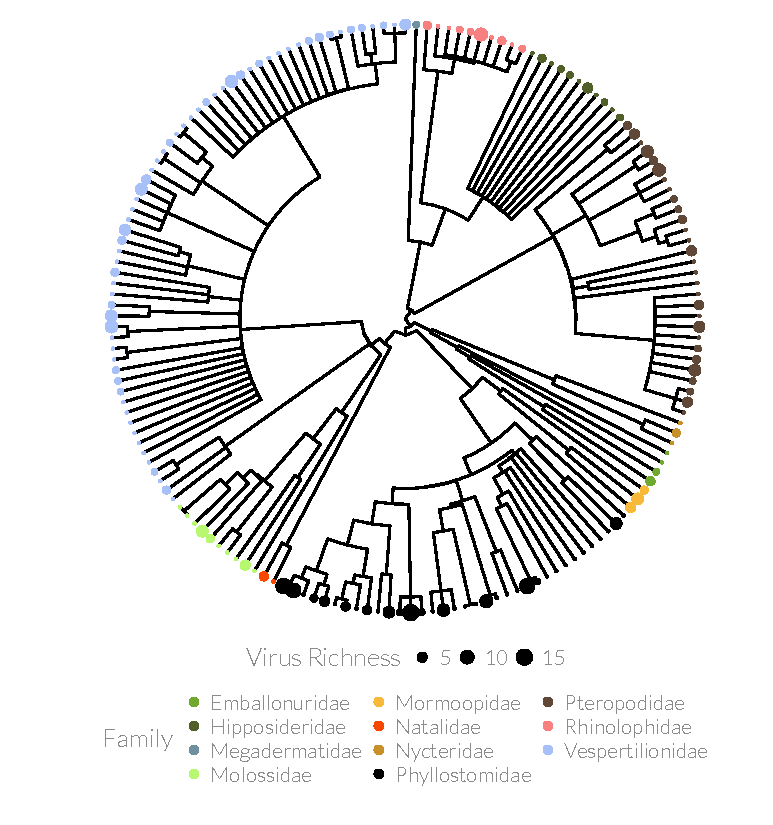
\includegraphics[width=1\textwidth,trim = 0cm 0cm 0cm 0cm]{figures/A-treePlot2-1} 

}

\caption[Pruned alternative phylogeny with dot size showing number of pathogens and colour showing family.]{
Phylogeny from \textcite{jones2005bats} (version 2) pruned to include all species used in the number of subspecies analysis.
Dot size shows the number of known viruses for that species and colour shows family.
Analyses run with this phylogeny gave qualitatively similar results to analyses using the phylogeny from \cite{bininda2007delayed}.
}\label{fig:treePlot2}
\end{figure}


\end{knitrout}









% Chapter 3 Appendix
\chapter{Appendix: Understanding how population structure affects pathogen richness in a mechanistic model of bat populations}
\chaptermark{Appendix: Population structure and pathogen richness: a mechanistic model}
\label{sims1Appendix}
%--------------------------------------------------------------------------------------------------------------------------------%
% Code for "Appendix C: Understanding how population structure affects pathogen richness in a mechanistic model of bat populations"
% Appendix for Chapter 3 of thesis "The role of population structure and size in determining bat pathogen richness"
% by Tim CD Lucas
%
% NB The file is numbered Appendix2 as Chapter 3 was previously Chapter 2 in the thesis.
%
%---------------------------------------------------------------------------------------------------------------------------------%


















% --------------------------------------------------------------------------- %
% Invading pathogen plots
% --------------------------------------------------------------------------- %




\begin{knitrout}\footnotesize
\definecolor{shadecolor}{rgb}{0.969, 0.969, 0.969}\color{fgcolor}\begin{figure}[t]

{\centering 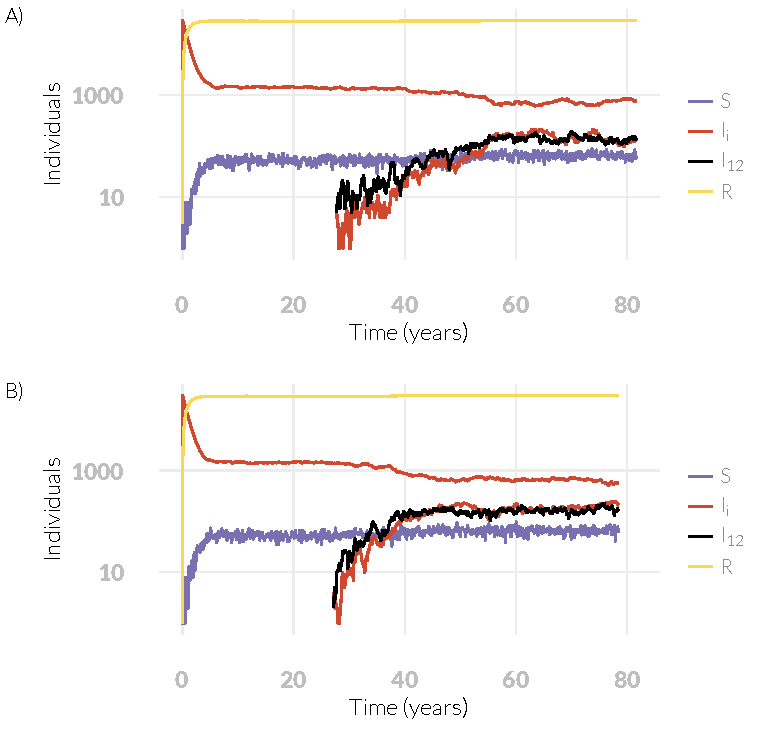
\includegraphics[width=\textwidth]{figure/A-plotsInvade-1} 

}

\caption[
Examples of simulated SIR dynamics with successfull invasions
]{
Two examples (A and B) of a successful invasion plotted on a logged $y$-axis.
The lines are coloured such that blue represents susceptibles, brown represents individuals infected with one pathogen (the two seperate brown lines are Pathogen 1 and 2), black represents co-infected individuals and yellow represents recovered and immune individuals.
Pathogen 2 is seeded after \SI{300000} events (approximately 30 years).
Simulations are run on a fully-connected network.
Parameter values are: dispersal rate = 0.1, transmission rate = 0.2.
All other parameters are as stated in Table~\ref{t:params}.
}\label{fig:plotsInvade}
\end{figure}


\end{knitrout}



% --------------------------------------------------------------------------- %
% No invasion plots
% --------------------------------------------------------------------------- %







\begin{knitrout}\footnotesize
\definecolor{shadecolor}{rgb}{0.969, 0.969, 0.969}\color{fgcolor}\begin{figure}[t]

{\centering 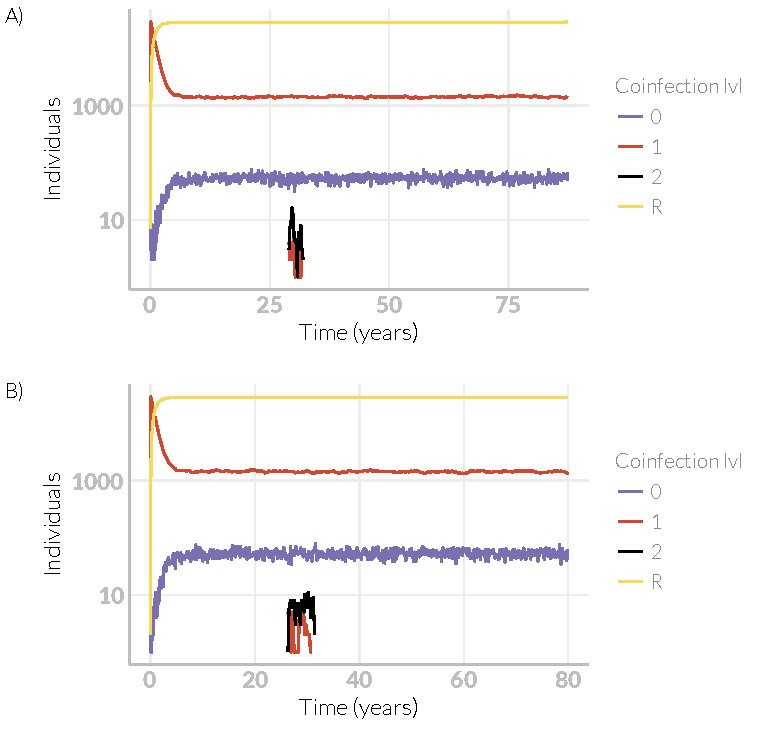
\includegraphics[width=\textwidth]{figure/A-plotsNoInvade-1} 

}

\caption[
Examples of simulated SIR dynamics with unsuccessfull invasions
]{
Two examples (A and B) of an unsuccessful invasion plotted on a logged $y$-axis.
The lines are coloured such that blue represents susceptibles, brown represents individuals infected with one pathogen (the two separate brown lines are Pathogen 1 and 2), black represents co-infected individuals and yellow represents recovered and immune individuals.
Pathogen 2 is seeded after \SI{300000} events (approximately 30 years).
It can be seen that after seeding Pathogen 2, there is a very short period before extinction as opposed to a long fade out of disease.
Simulations are run on a fully-connected network.
Parameter values are: dispersal rate = 0.1, transmission rate = 0.2.
All other parameters are as stated in Table~\ref{t:params}.
}\label{fig:plotsNoInvade1}
\end{figure}

\begin{figure}[t]

{\centering 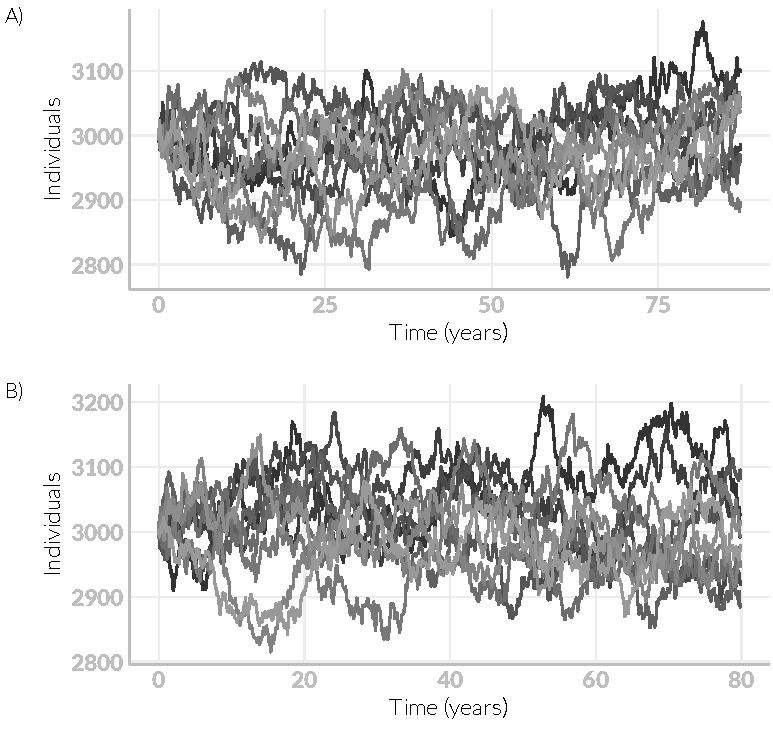
\includegraphics[width=0.8\textwidth]{figure/A-plotsNoInvade-2} 

}

\caption[
Examples of colony size dynamics
]{
Two examples (A and B) of the change in colony sizes throughout a simulation (note the truncated $y$-axis).
The size of each colony changes as a random walk.
However, given the length of the simulations, there is little risk of colonies going extinct or becoming very large.
Birth and death rate are equal and set to 0.05, giving a generation time of 20 years.
The metapopulation network is fully-connected and the dispersal rate is 0.1 per year.
The starting colony size is \SI{3000}.
}\label{fig:plotsNoInvade2}
\end{figure}


\end{knitrout}














% ------------------------------------------------------------------ %
% Topology Sims
% ------------------------------------------------------------------ %

















% ------------------------------------------------ %
% Raw data tables
% ------------------------------------------------ %








































\clearpage
% latex table generated in R 3.3.1 by xtable 1.8-2 package
% Mon Jul 25 00:04:16 2016
\begin{table}[ht]
\centering
\caption[
Raw data for dispersal simulations
  ]{
Raw data for dispersal simulations.
The relevant parameters are shown along with the number of invasions and the number of simulations.
$\beta$ is the transmission rate.
} 
\label{B-disp}
\begingroup\small
\begin{tabular}{@{}rrrr@{}}
  \toprule
$\beta$ & Dispersal & Invasions & Sims \\ 
  \midrule
0.1 & 0.000 & 0 & 100 \\ 
  0.1 & 0.001 & 1 & 101 \\ 
  0.1 & 0.010 & 0 & 100 \\ 
  0.1 & 0.100 & 0 & 99 \\ 
  0.2 & 0.000 & 4 & 100 \\ 
  0.2 & 0.001 & 42 & 126 \\ 
  0.2 & 0.010 & 41 & 126 \\ 
  0.2 & 0.100 & 63 & 123 \\ 
  0.3 & 0.000 & 47 & 100 \\ 
  0.3 & 0.001 & 113 & 125 \\ 
  0.3 & 0.010 & 113 & 126 \\ 
  0.3 & 0.100 & 112 & 124 \\ 
  0.4 & 0.000 & 75 & 100 \\ 
  0.4 & 0.001 & 96 & 100 \\ 
  0.4 & 0.010 & 98 & 100 \\ 
  0.4 & 0.100 & 96 & 100 \\ 
   \bottomrule
\end{tabular}
\endgroup
\end{table}





% latex table generated in R 3.3.1 by xtable 1.8-2 package
% Mon Jul 25 00:04:16 2016
\begin{table}[ht]
\centering
\caption[
Raw data for topology simulations
  ]{
Raw data for topology simulations.
The relevant parameters are shown along with the number of invasions and the number of simulations.
$\beta$ is the transmission rate.
} 
\label{B-topo}
\begingroup\small
\begin{tabular}{@{}rllr@{}}
  \toprule
$\beta$ & Topology & Invasions & Sims \\ 
  \midrule
0.1 & Unconnected & 0 & 100 \\ 
  0.1 & Minimally & 1 & 101 \\ 
  0.1 & Fully & 1 & 99 \\ 
  0.2 & Unconnected & 4 & 100 \\ 
  0.2 & Minimally & 30 & 100 \\ 
  0.2 & Fully & 28 & 100 \\ 
  0.3 & Unconnected & 47 & 100 \\ 
  0.3 & Minimally & 94 & 100 \\ 
  0.3 & Fully & 88 & 100 \\ 
  0.4 & Unconnected & 75 & 100 \\ 
  0.4 & Minimally & 97 & 100 \\ 
  0.4 & Fully & 99 & 100 \\ 
   \bottomrule
\end{tabular}
\endgroup
\end{table}









% Chapter 5 Appendix
\chapter{Appendix: A generalised random encounter model for estimating animal density with remote sensor data}
\chaptermark{Appendix: A generalised random encounter model for estimating animal density}
\label{gremAppendix}
  

\clearpage
\section{Table of symbols}

%move to appendix
\begin{table}[h!]
\centering
\begin{tabular}{lll}
Symbol 	& Description & Units\\\hline
$\theta$	& Sensor width & \SI{}{\radian} \\
$\alpha$	& Animal signal width & \SI{}{\radian} \\
$x_i$	        & Focal angle, $i \in \{1,2,3,4\} $ 	& \SI{}{\radian}\\
$r$ 		& Detection distance & \SI{}{\meter}\\
$\bar{p}$ 		& Average profile width & \SI{}{\meter}\\
$p$ 		& A specific profile width & \SI{}{\meter}\\
$v$		& Velocity & \SI{}{\meter\per\second}\\
$t$		& Time & \SI{}{\second}\\
$z$		& Number of detections & -\\
$D$		& Animal density & \SI{}{\per\meter\squared} \\
$T$ 		& Step length & \SI{}{\second}\\
$N$ 		& Number of steps per simulation & -\\
$d$ 		& Distance moved in a time step & \SI{}{\meter}\\
$S$ 		& Probability of remaining stationary & -\\
$A$ 		& Maximum turning angle & \SI{}{\radian}\\
\\
\end{tabular}
\caption{List of symbols used to describe the gREM and simulations. `-' means the quantity has no units.}
\label{t:paras}
\end{table}

\clearpage

\section{Supplementary Methods}
\subsection{Introduction}
\lettr{T}hese supplementary methods derive all the models used. 
For continuity, the gas model derivation is included here as well as in the main text. 
The calculation of all integrals use in the gREM is included in the Python script S3. 



\subsection{Gas model} \label{gas}

Following \cite{yapp1956theory}, we derive the gas model where sensors can capture animals in any direction and animal signals are detectable from any direction ($ \theta =  2\pi$ and $ \alpha =  2\pi$).
We assume that animals are in a homogeneous environment, and move in straight lines of random direction with velocity $v$.
We allow that our stationary sensor can capture animals at a detection distance $r$ and that if an animal moves within this detection zone they are captured with a probability of one, while animals outside the zone are never captured.




\begin{figure}[t]
  \centering
{
  \subfloat[$x_1$\label{fig:x1}]{
    \centering
    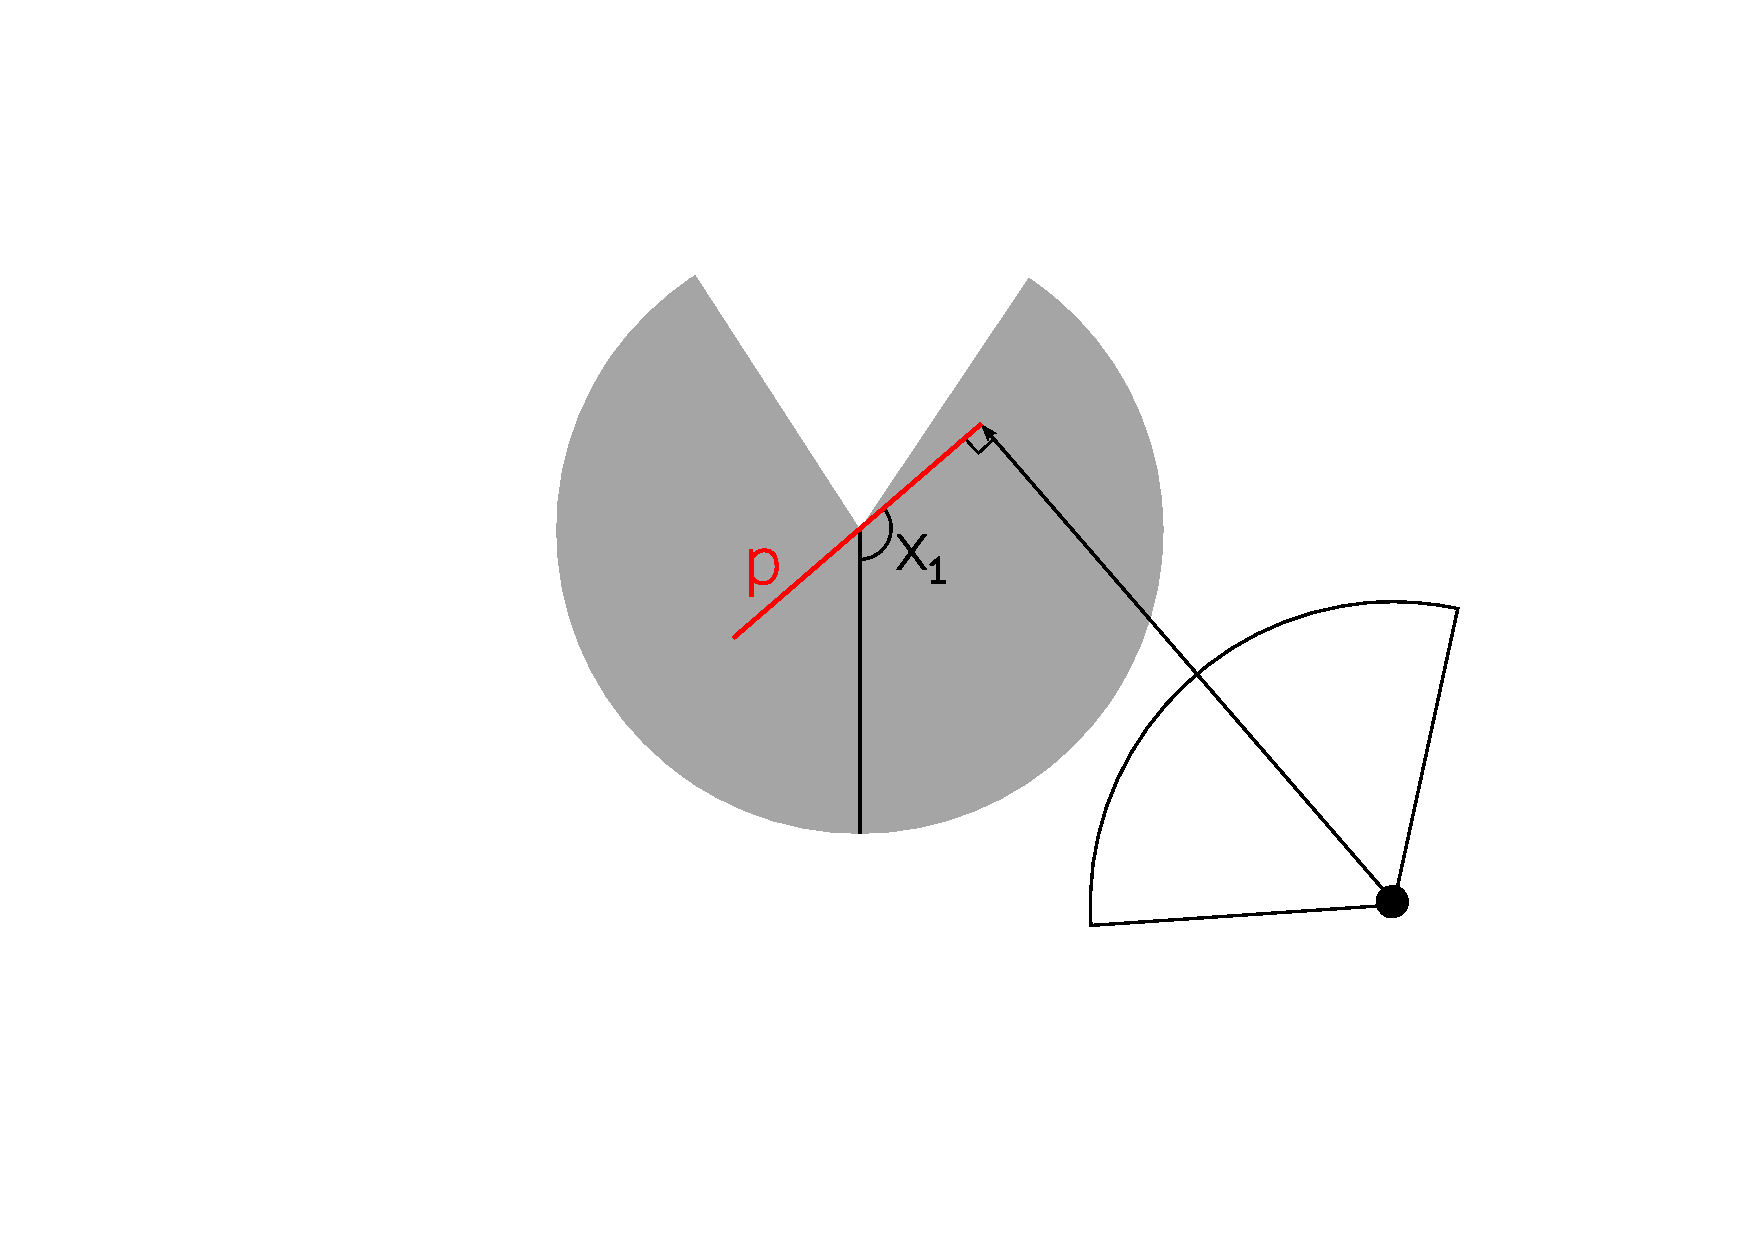
\includegraphics[width=.44\textwidth, trim=2cm 1cm 2cm 3cm]{imgs/x1.pdf}
  }
  \subfloat[$x_2$\label{fig:x2}]{
    \centering
    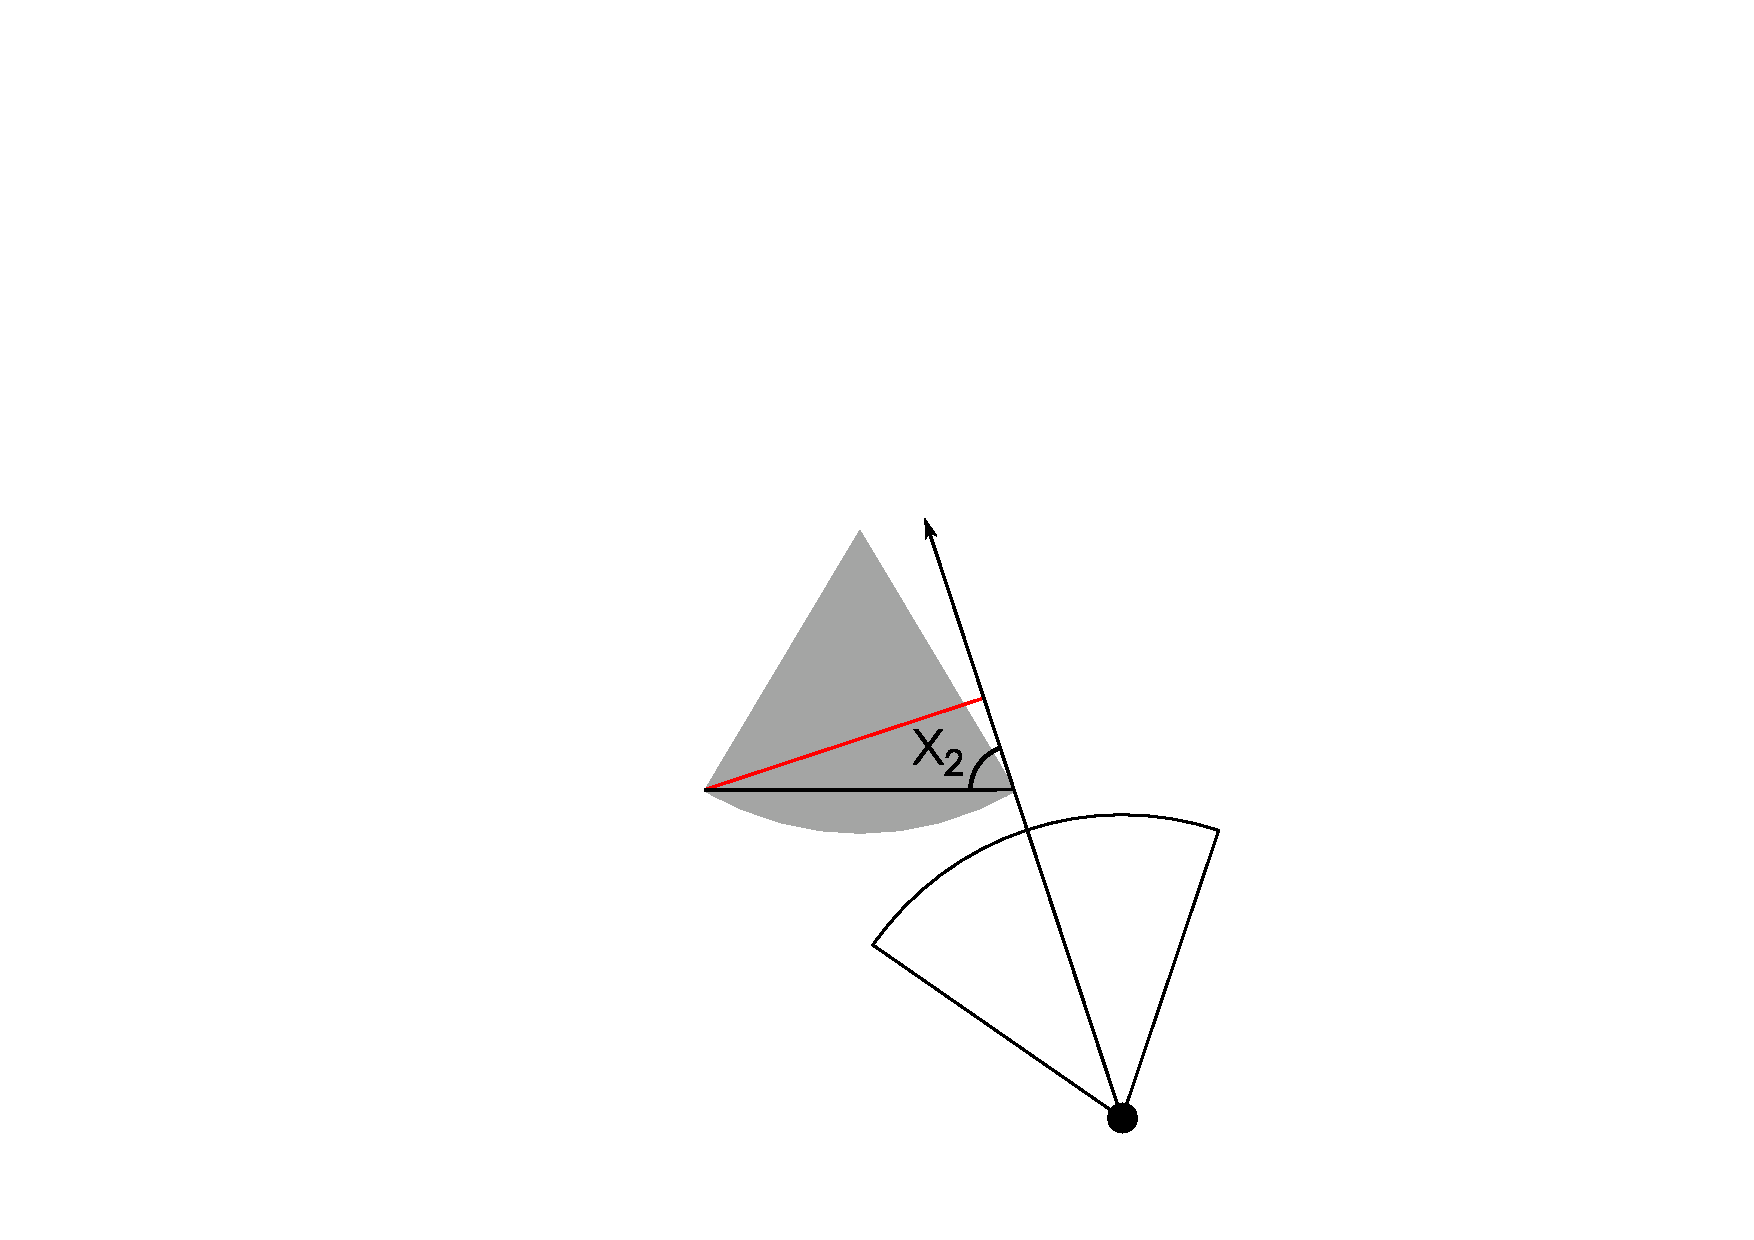
\includegraphics[width=.29\textwidth, trim=9cm 2cm 9cm 6cm]{imgs/x2.pdf}
  }
  
  \subfloat[$x_3$\label{fig:x3}]{
    \centering
    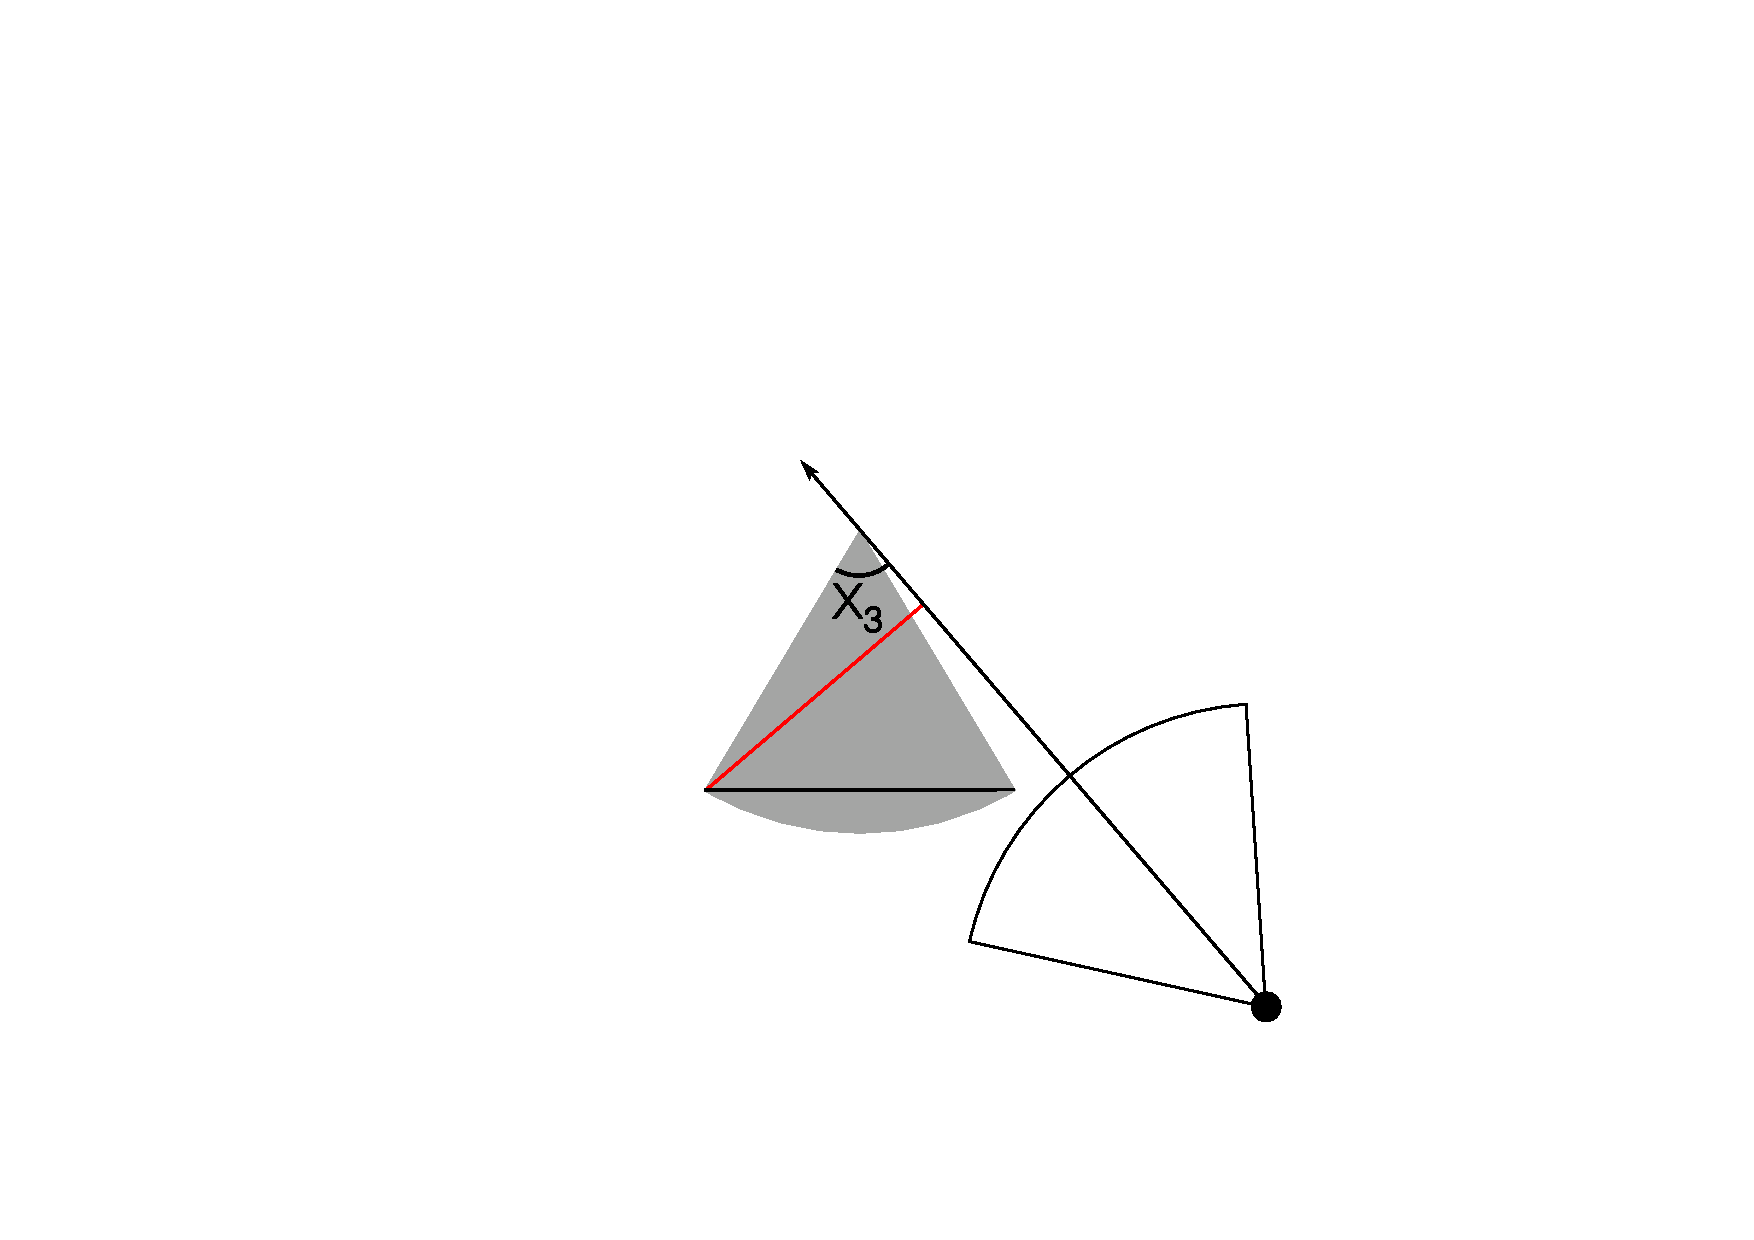
\includegraphics[width=.29\textwidth, trim=9cm 2cm 9cm 6cm]{imgs/x3.pdf}
  }
  \subfloat[$x_4$\label{fig:x4}]{
    \centering
    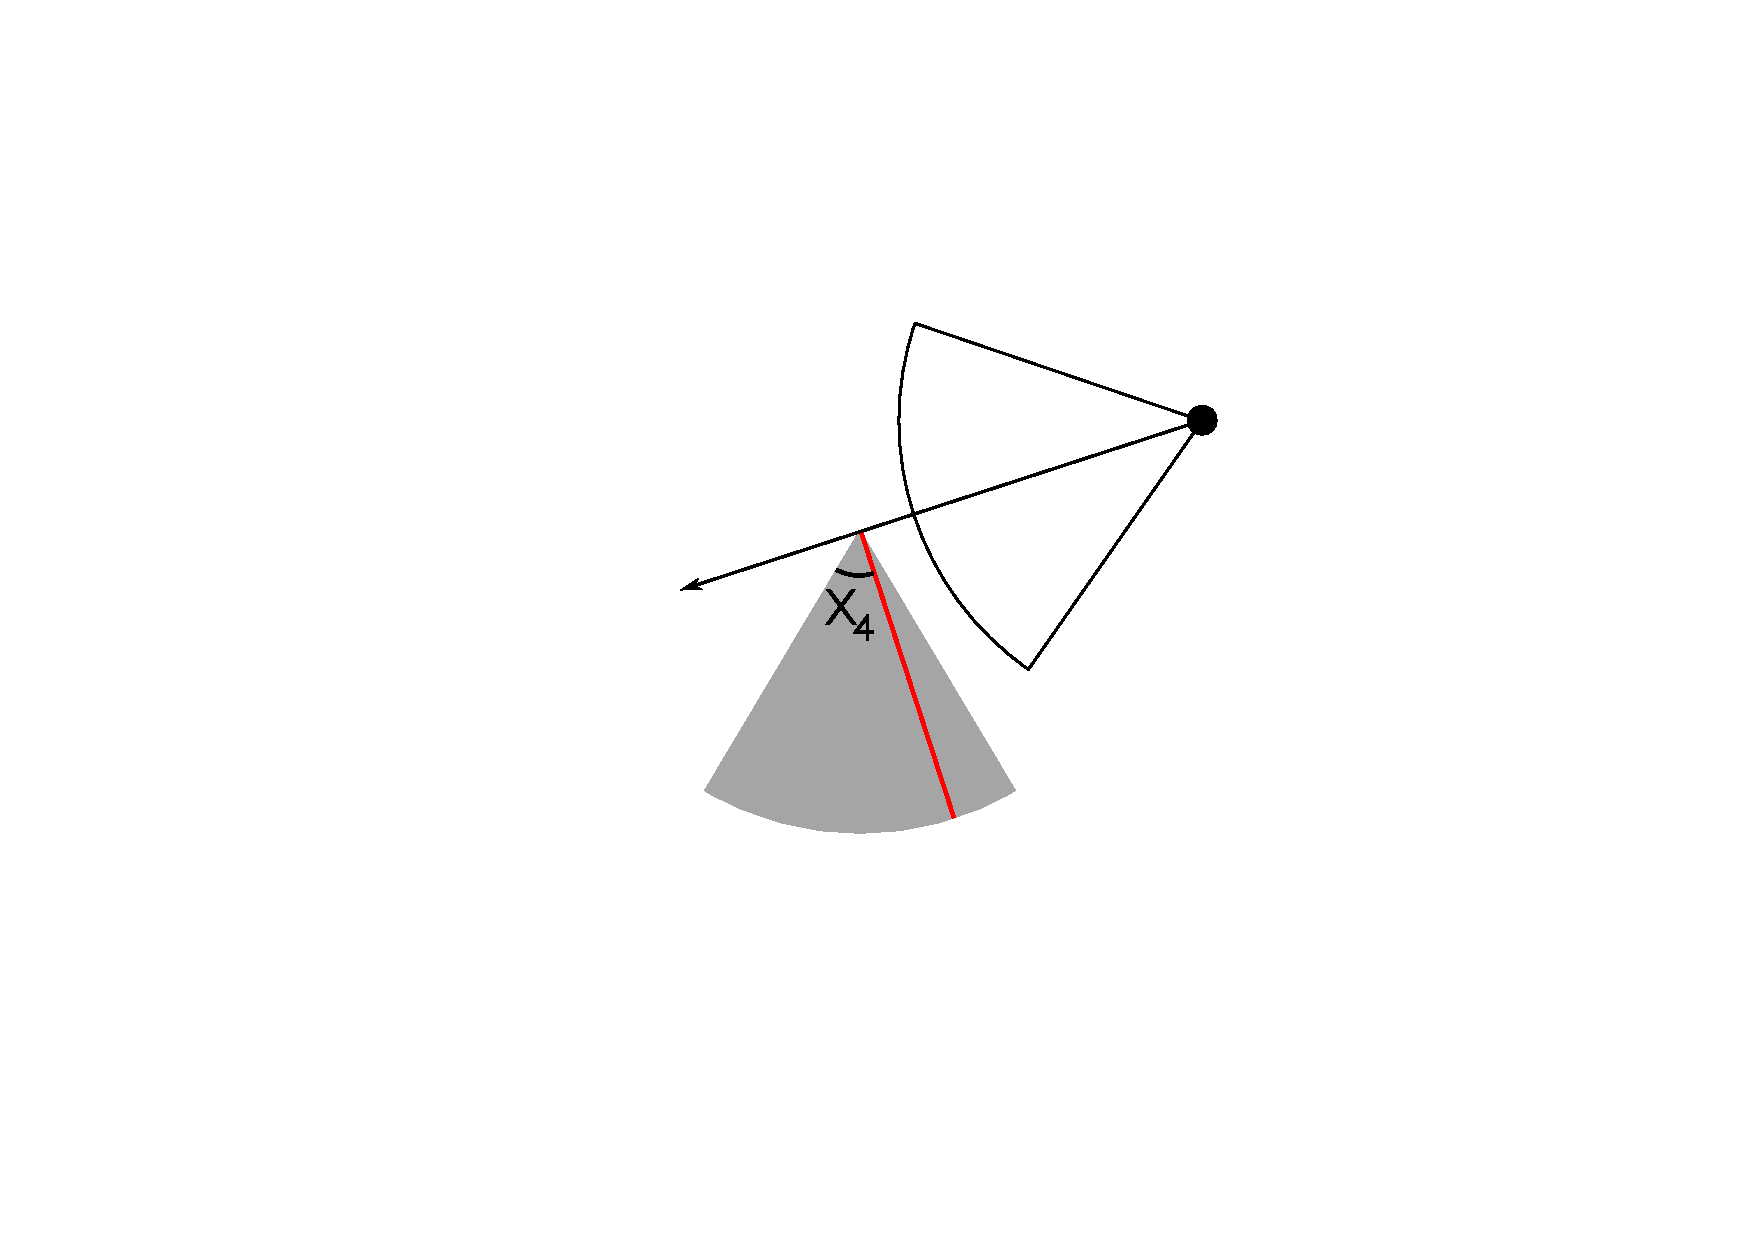
\includegraphics[width=.29\textwidth, trim=7cm 2cm 11cm 6cm]{imgs/x4.pdf}
  }
}
\caption[The location of the focal angles $x_{i\in[1,4]}$]{
The location of the focal angles $x_{i\in[1,4]}$.
$x_1$ is used in SE and NE models (including the gas model).
$x_2$ -- $x_4$ are used in NW and SW models.
The sector shaped detection region is shown in grey.
Animals are filled black circles and the animal signal is an unfilled sector.
The animals direction of movement is indicated with an arrow.
The profile $p$ is shown with a red line.
(a) Animal is directly approaching the sensor at $x_1$ = $\frac{\pi}{2}$.
(b) Animal is directly approaching the sensor at $x_2$ = $\frac{\pi}{2}$.
$x_2$ then decreases until the profile is perpendicular to the edge of the detection region.
(c) When the profile is perpendicular to the edge of the detection region, $x_3 = \theta$.
(d) $x_4$ measures the angle between the left side of the detection region and the profile.}

\label{fig:xis}
\end{figure}



In order to derive animal density, we need to consider relative velocity from the reference frame of the animals.
Conceptually, this requires us to imagine that all animals are stationary and randomly distributed in space, while the sensor moves with velocity $v$.
If we calculate the area covered by the sensor during the survey period we can estimate the number of animals the sensor should capture.
As a circle moving across a plane, the area covered by the sensor per unit time is $2rv$.
The number of expected captures, $z$, for a survey period of $t$, with an animal density of $D$ is $z = 2rvtD$.
To estimate the density, we rearrange to get $D = z/2rvt$.

\subsubsection{gREM derivations for different detection and signal widths}
Different combinations of $\theta$ and $\alpha$ would be expected to occur (\emph{e.g.}, sensors have different detection widths and animals have different signal widths).
For different combinations $\theta$ and $\alpha$, the area covered per unit time is no longer given by $2rv$.
Instead of the size of the sensor detection zone having a diameter of $2r$, the size changes with the approach angle between the sensor and the animal.
For any given signal width and detector width and depending on the angle that the animal approaches the sensor, the width of the area within which an animal can be detected is called the profile, $p$.
The size of the profile (averaged across all approach angles) is defined as the average profile $\bar{p}$.
However, different combinations of $\theta$ and $\alpha$ need different equations to calculate $\bar{p}$.
This $\bar{p}$ is the only thing that changes 

We have identified the parameter space for the combinations of $\theta$ and $\alpha$ for which the derivation of the equations are the same (defined as sub-models in the gREM) (Figure~\ref{fig:equalRegions}).
For example, the gas model becomes the simplest gREM sub-model (upper right in Figure~\ref{fig:equalRegions}) and the REM from \cite{rowcliffe2008estimating} is another gREM sub-model where $\theta<\pi/2$ and $\alpha = 2\pi$.

Models with $\theta = 2\pi$ are described first (the gas model described above and SE1).
Then models with $\theta > \pi$ are described (NE then SE).
Finally models with $\theta < \pi$ (NW then SW) are described.

\subsection{Model SE1} \label{SE1}
SE1 is very similar to the gas model except that because $\alpha \le \pi$ the profile width is no longer $2r$ but is instead limited by the width of the animal signal.
We therefore get a profile width of $2r\sin(\alpha/2)$ instead.

\begin{align}
    \bar{p}_{\text{\tiny{SE1}}} =&\frac{1}{\pi} \int\limits_{\frac{\pi}{2}}^{\frac{3 \pi}{2}}2 r \sin{\left (\frac{\alpha}{2} \right )}\;\mathrm{d}x_{1}\label{pSE1Def}\\
    \bar{p}_{\text{\tiny{SE1}}}  =& 2 r \sin{\left (\frac{\alpha}{2} \right )}\label{pSE1Sln}
\end{align}
This profile is integrated over the interval $[\frac{\pi}{2}, \frac{3\pi}{2}]$ which is $\pi$ radians of rotation starting with the animal moving directly towards the sensor (Figure~\ref{fig:xis}a).

\subsection{ Models NE1--3} \label{NE}

When the detection zone is not a circle, we have more complex profiles  and need to explicitly write functions for the width of the profile for every approach angle.
We then use these functions to find the average profile width $\bar{p}$ for all approach angles by integrating across all $2\pi$ angles of approach and dividing by $2\pi$.




\begin{figure}[t]
  \centering
{
  \subfloat[\label{fig:NELimit}]{
    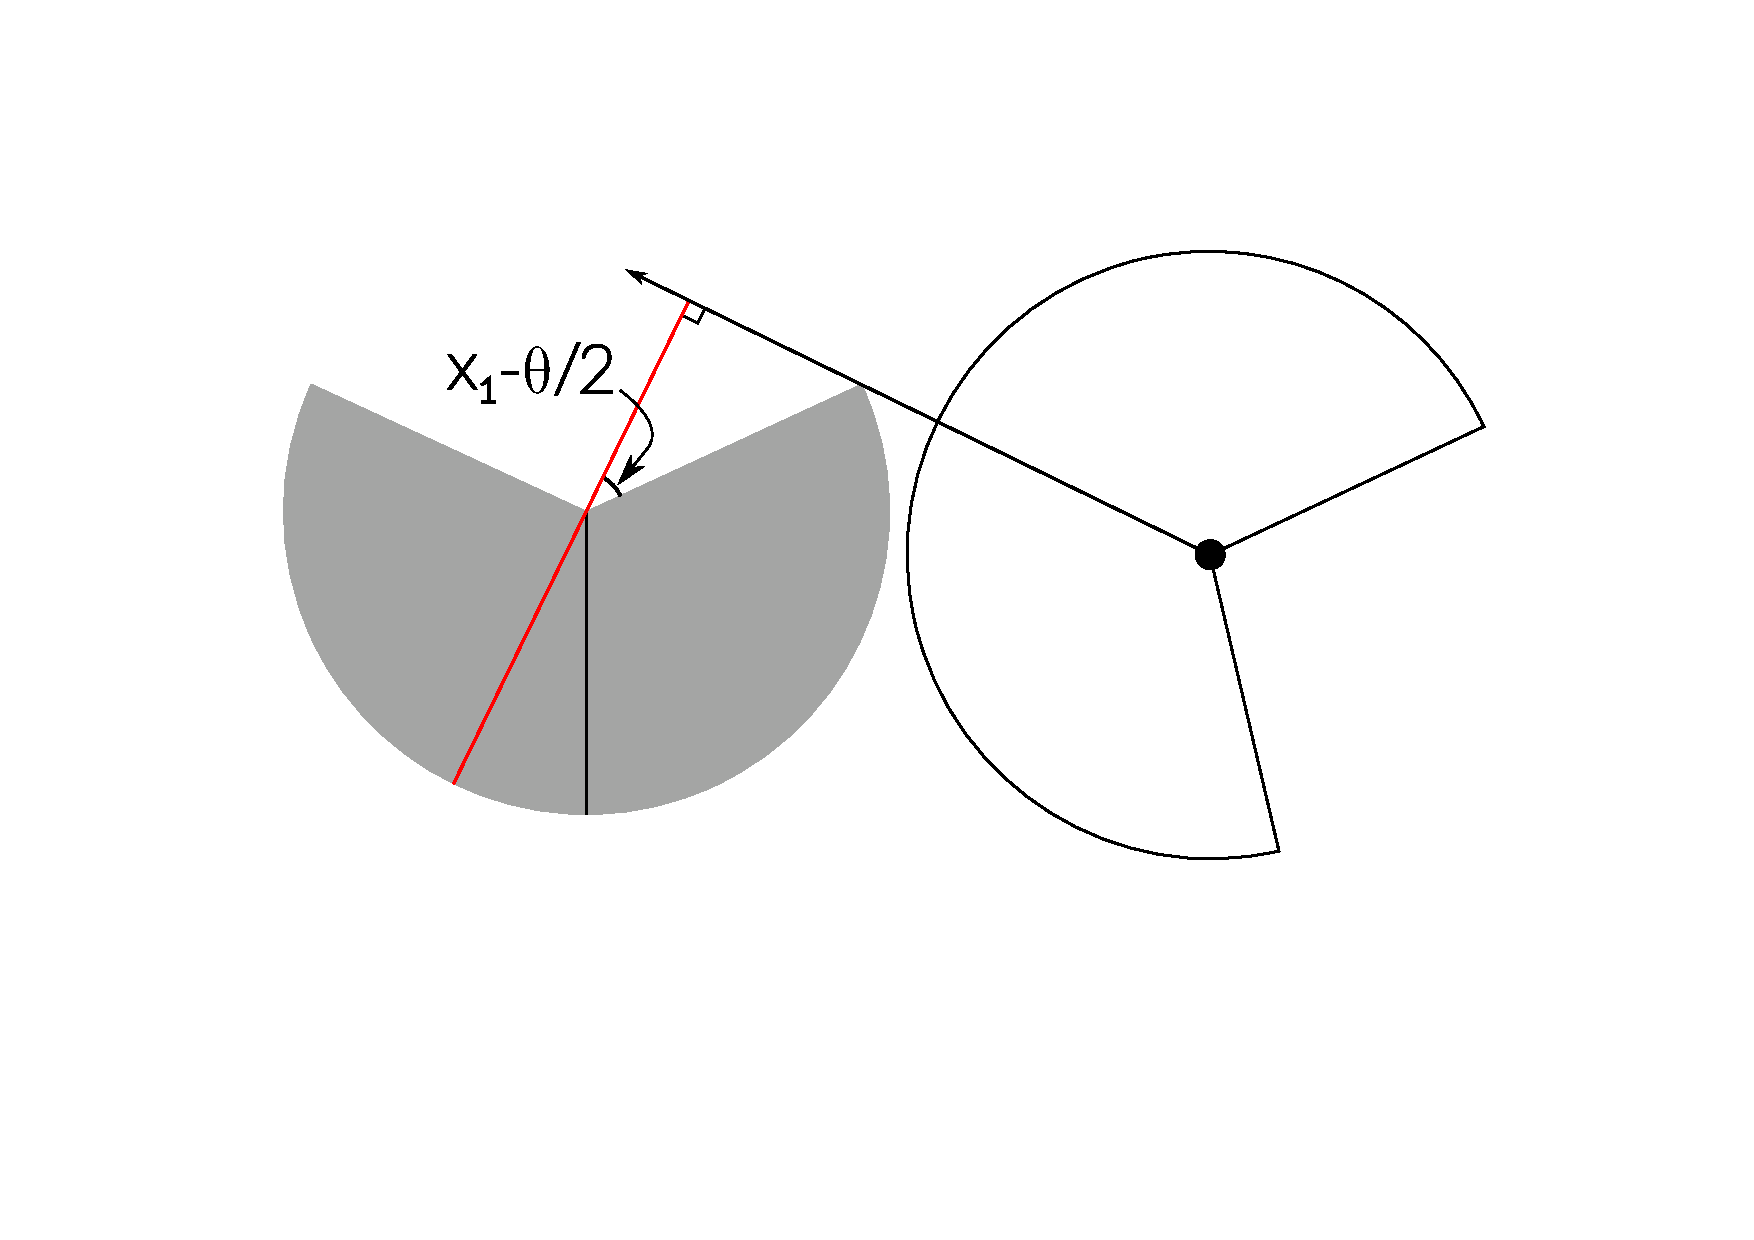
\includegraphics[width=.3\textwidth, trim=5cm 3cm 4cm 1cm]{imgs/ne2.pdf}
  } 
  \subfloat[\label{fig:NE3third}]{
    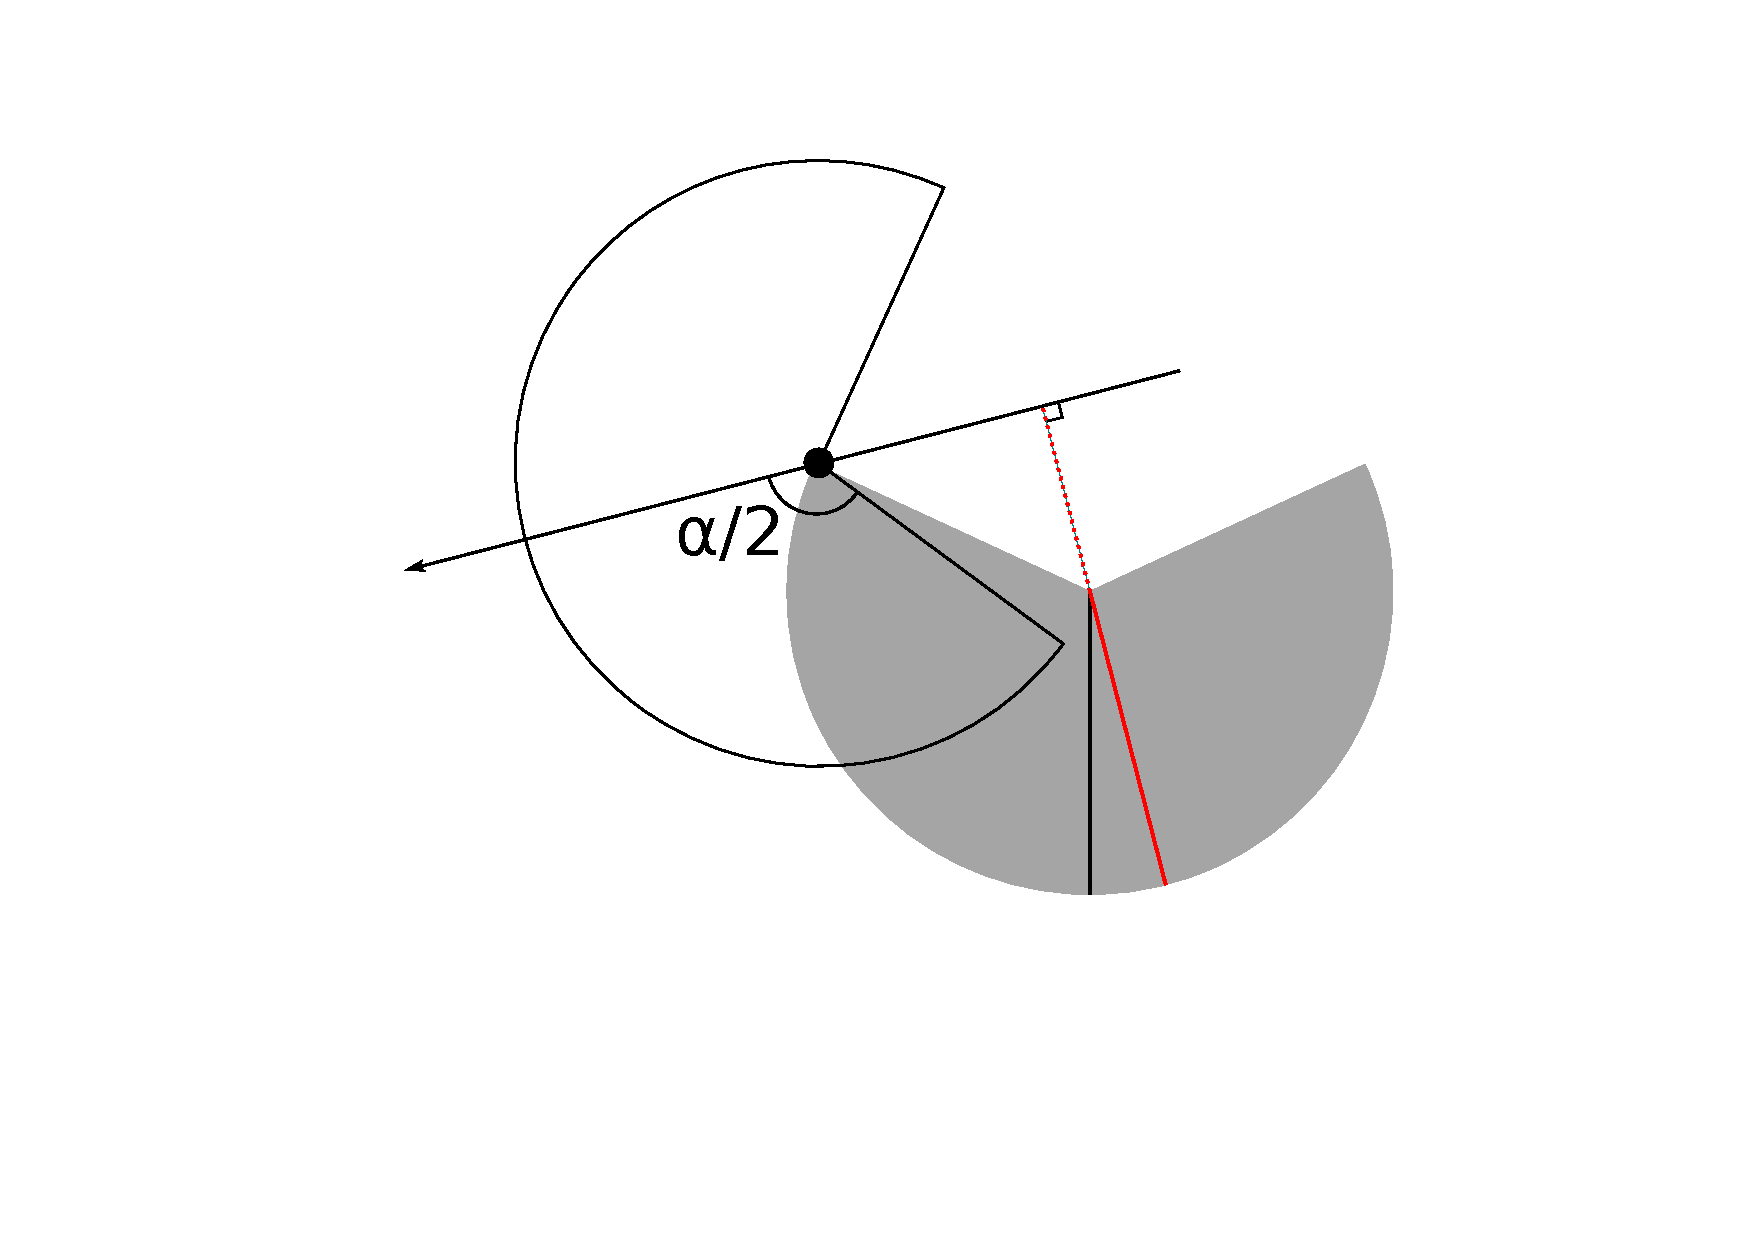
\includegraphics[width=.3\textwidth, trim=4cm 2cm 6cm 0cm]{imgs/ne33.pdf}
  }
  \subfloat[\label{fig:NE3fourth}]{
    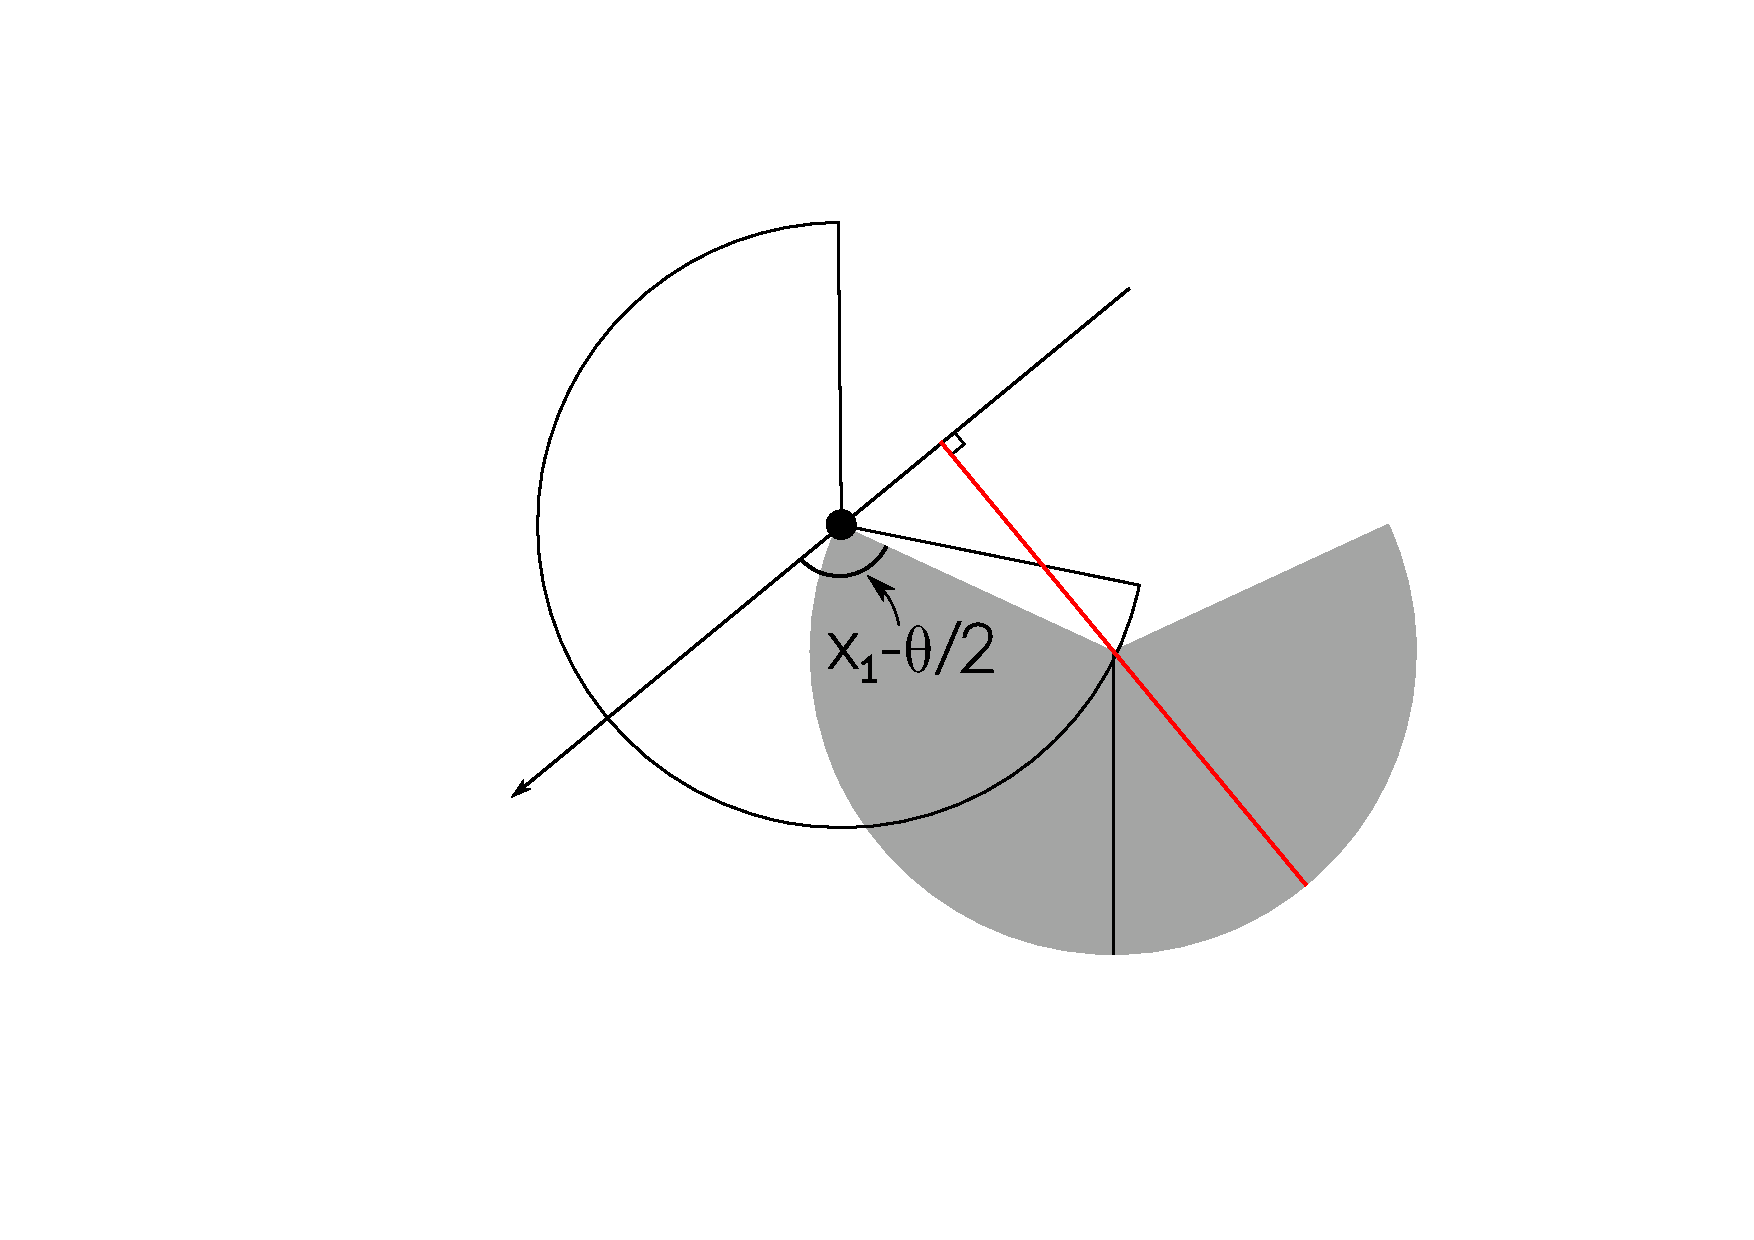
\includegraphics[width=.3\textwidth, trim=5cm 1cm 4cm 1cm]{imgs/ne34.pdf}
  }
}
\caption[Three of the integrals in NE models]{
Three of the integrals in NE models.
The sector shaped detection region is shown in grey.
Animals are filled black circles and the animal signal is an unfilled sector.
The animals direction of movement is indicated with an arrow.
The profile $p$ is shown with a red line.
Dashed red lines indicate areas where animals cannot be detected.
(a) The second integral in NE with width $r + r\cos(x_1 - \theta/2)$.
(b) The third integral in NE3.
$\alpha/2$ is labelled.
As it is small, animals to the right of the detector cannot be detected.
(c) After further rotation, $\alpha/2$ is now bigger than the angle shown and animals to the right of the detector can again be detected.
}
\label{fig:NE}
\end{figure}


\begin{figure}[t]
        \centering
        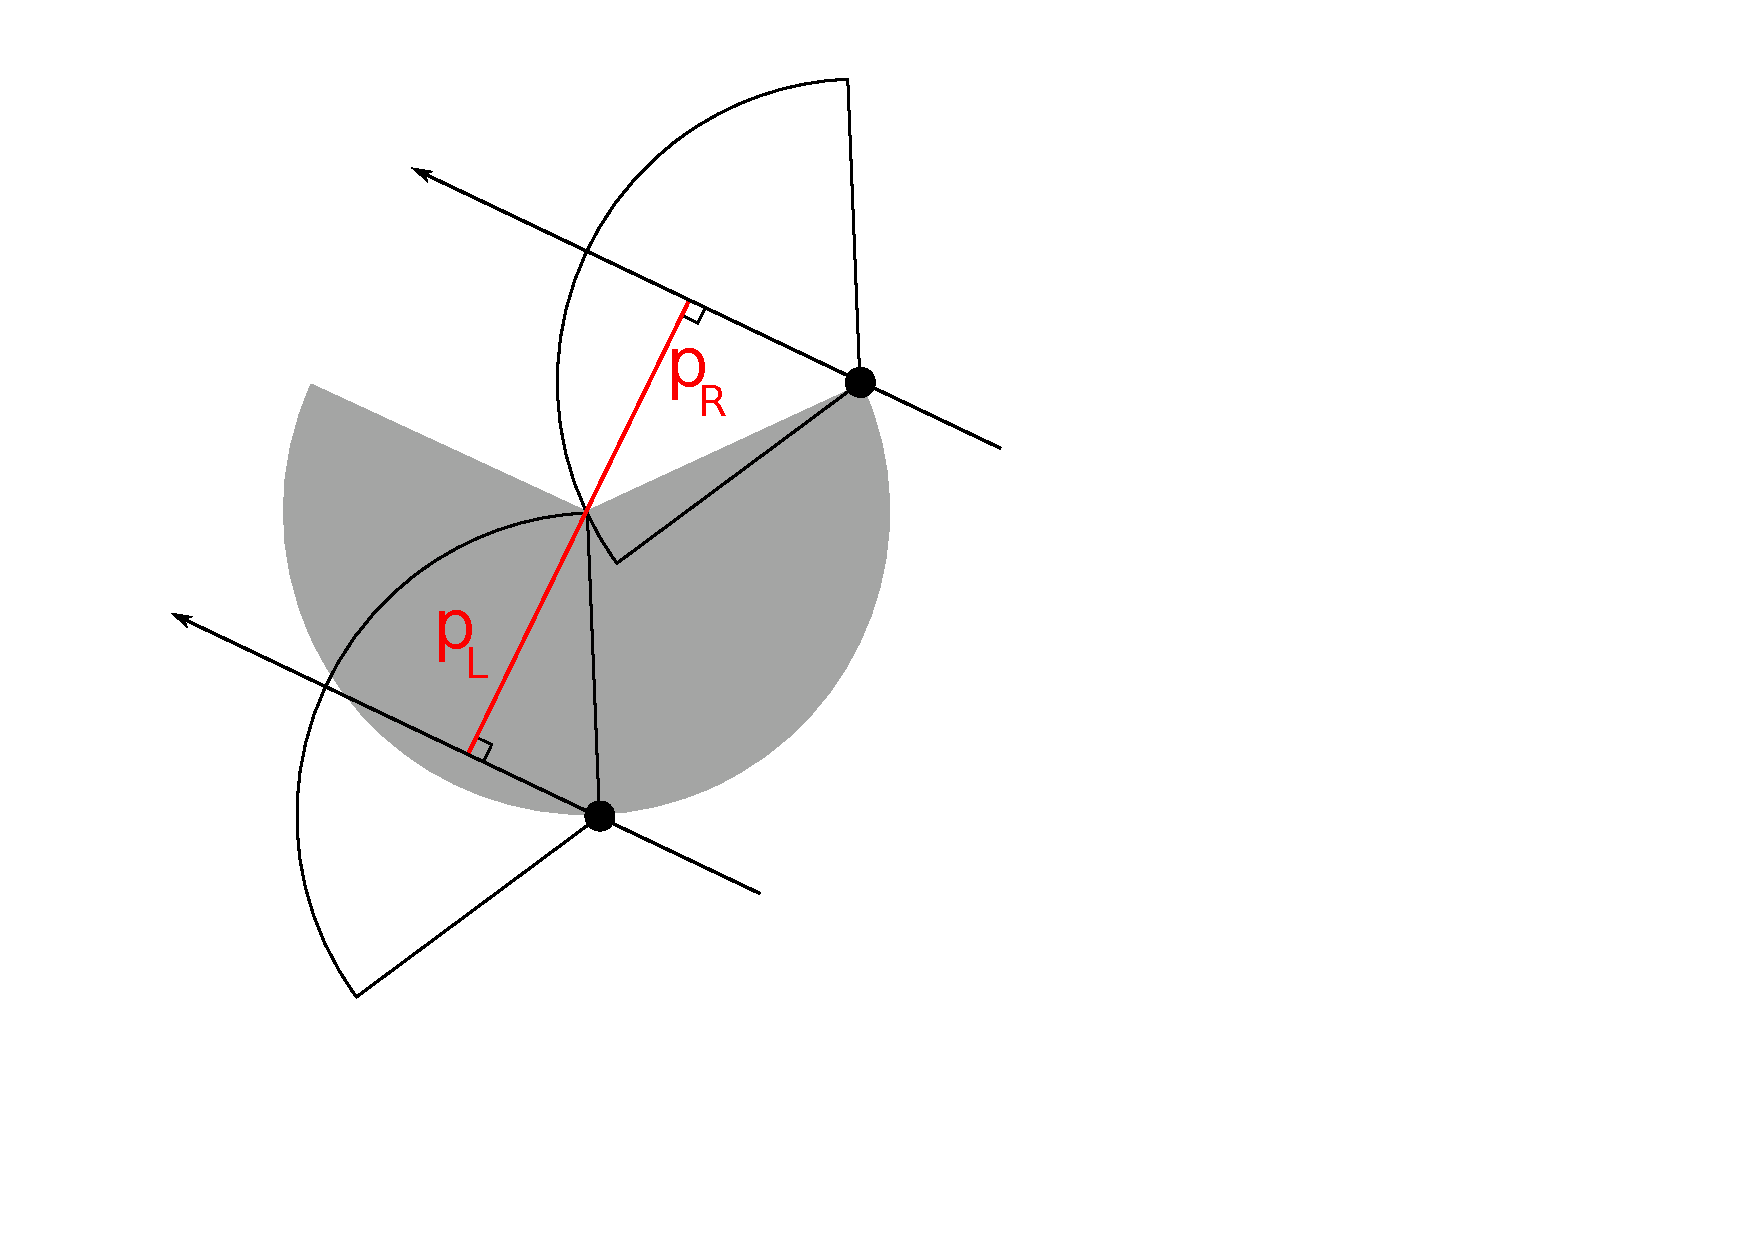
\includegraphics[width=0.35\textwidth, trim=1cm 4cm 9cm 1cm]{imgs/se3.pdf}
\caption[The second integral in SE]{The second integral in SE.
The right side of the profile ($p_R$) is limited by the size of the sensor region  while the left side of the profile ($p_L$) is limited by the size of the signal width.
The full profile has width $p = r\sin(\alpha/2) +r\cos(\theta/2-x_1)$.
The sector shaped detection region is shown in grey.
Animals are filled black circles and the animal signal is an unfilled sector.
The animals direction of movement is indicated with an arrow.
The profile $p$ is shown with a red line.
  }
\label{fig:se3}
\end{figure}

There are three submodels within quadrant NE (Figure~\ref{fig:equalRegions}).
Note that NE1 covers the area $\alpha=2\pi$ as well as the triangle below it as these two models are specified exactly the same, rather than happening to have equal results.

These models have up to five profiles.

\begin{enumerate}
\item The profile width starts, from $x_1=\frac{\pi}{2}$ as $2r$.
\item At $x_1 = \theta/2$, the right hand side of the profile cannot be $r$ wide as the corner of the `blind spot' limits its size to being $r\cos(x_1 - \theta/2)$ wide (Figure~\ref{fig:NELimit}).

\item The third profile is only found in NE3.
If $\alpha < 4\pi - 2\theta$, then at $x_1=\theta/2 + \pi/2$, when the profile is perpendicular to the edge of the blind spot, the whole right side of the profile is invisible to the sensor (Figure~\ref{fig:NE3third}).
This gives a profile size of just $r$.

\item At some point, the sensor can detect animals once they have passed the blind spot giving a profile width of $r + r\cos(x_1 + \theta/2)$ (Figure~\ref{fig:NE3fourth}).
From $x_1=\pi$, if the animal signal is wide enough to be detected in this area, this is the wider profile.
This then defines the split between NE1 and NE2.
In NE1, with $\alpha > 3\pi - \theta$, the animal signal is wide enough that at $x_1=\pi$ the animal can immediately be detected past the blind spot and so this profile is used.
In NE2, with $\alpha < 3\pi - \theta$, the latter profile is reached at $5\pi/2 - \theta/2 - \alpha/2$.

\item Finally, common to all three models, at $x_1 = 2\pi - \theta/2$ the profile becomes a full $2r$ once again.
\label{NElist5}
\end{enumerate}



\subsubsection{Model NE1} \label{NE1}

Submodel NE1 exists within the area bounded by $\alpha\le2\pi$, $\theta\le2\pi$ and $\alpha \ge 3\pi - \theta$ (Figure~\ref{fig:equalRegions}).
It has four profiles; it does not include the $r$ profile at $x_1=\pi$ (profile described in point (3) in Section \ref{NE}).
Furthermore, $\theta$ is wide enough that the $r + r\cos(x_1 + \theta/2)$ profile starts at $\pi$.
This then gives us


\input{latexFiles/pNE1.tex}





\subsubsection{Model NE2} \label{NE2}

Model NE2 is bounded by $\alpha \le 3\pi - \theta$, $\alpha \ge 4\pi - 2\theta$ and $\alpha \ge \pi$ (Figure~\ref{fig:equalRegions}).
It is the same as NE1 except that the third profile starts at $5\pi/2 - \theta/2 - \alpha/2$ instead of at $\pi$ which is reflected in the different bounds in the second and third integral.

\input{latexFiles/pNE2.tex}

\subsubsection{Model NE3} \label{NE3}

Model NE3 is bound by $\alpha \le 4\pi - 2\theta$, $\alpha \ge \pi$ and $\theta \ge \pi$ (Figure~\ref{fig:equalRegions}).
It is the same as NE2 except that it contains the extra profile with width $r$ (third integral).

\input{latexFiles/pNE3.tex}




\subsection{Models SE2--4} \label{SE}

Quadrant SE contains three submodels excluding SE1  (Figure~\ref{fig:equalRegions}).
The differences between these three models are similar to the differences between the models in NE.
There are four possible profiles.
\begin{enumerate}
\item As $\alpha$ is less than $\pi$ the profile is smaller than $2r$, even when the sensor width is a full diameter.
The profile width starts as $2r\sin(\alpha/2)$.
\item Similar to NE, at a certain point the blind spot of the sensor area limits the profile width on one side.
This gives a profile width of $r\sin(\alpha/2) + r\cos(x_1 - \theta/2)$ (Figure~\ref{fig:se3}).
\item Also similar to NE, there can be a point where the right side of the profile is 0 giving a profile width of $r\sin(\alpha/2)$.
\item If $\alpha \le 2\pi - \theta$, then at $x_1 = \theta/2 + \pi/2 + \alpha/2 $ the profile width becomes 0.
This inequality distinguishes between SE3 and SE4.
\item The third profile $r\sin(\alpha/2)$ starts at $\theta/2 + \pi/2$ while at $5\pi/2 - \alpha/2 - \theta/2$ the profile returns to size $2r\sin(\alpha/2)$.
If $\theta/2 + \pi/2 \ge 5\pi/2 - \alpha/2 - \theta/2$ we go straight into the  $2r\sin(\alpha/2)$ profile and miss the $r\sin(\alpha/2)$ profile.
 SE2 and SE3 are separated by this inequality which simplifies to $\alpha \le 4\pi - 2\theta$.

\end{enumerate}





\subsubsection{Model SE2} \label{SE2}

SE2 is bounded by $\alpha \ge 4\pi - 2\theta$, $\alpha \le \pi$ and $\theta \le 2\pi$ (Figure~\ref{fig:equalRegions}).
As $\alpha \ge 4\pi - 2\theta$, there is no $r\sin(\alpha/2)$ profile.
As $\alpha \le 4\pi - 2\theta$, the profile returns to $2r\sin(\alpha/2)$ rather than going to 0.
These integrals relate to profiles (1), (2) and (5) in Section \ref{SE}.

\input{latexFiles/pSE2.tex}


\subsubsection{Model SE3} \label{SE3}

SE3 is bounded by $4\pi - 2\theta \le \alpha \le 4\pi - 2\theta$ and $\alpha \le \pi$ (Figure~\ref{fig:equalRegions}).
Therefore there is a $r\sin(\alpha/2)$ profile but no $0r$ profile.
This relates to profiles (1), (2), (3) and (5) above.

\input{latexFiles/pSE3.tex}

\subsubsection{Model SE4} \label{SE4}

Finally SE4 is bounded by  $\alpha \le 4\pi - 2\theta $, $\alpha\le\pi$ and $\theta \le \pi$ (Figure~\ref{fig:equalRegions}).
It is the same as SE3 except that the profile becomes 0 rather than returning to $2r\sin(\alpha/2)$.
This relates to profiles (1), (2), (3) and (4) above though profile (4) with width 0 is not shown.

\input{latexFiles/pSE4.tex}


\begin{figure}[t]
  \centering
{
  \subfloat[\label{fig:NW1AT}]{
    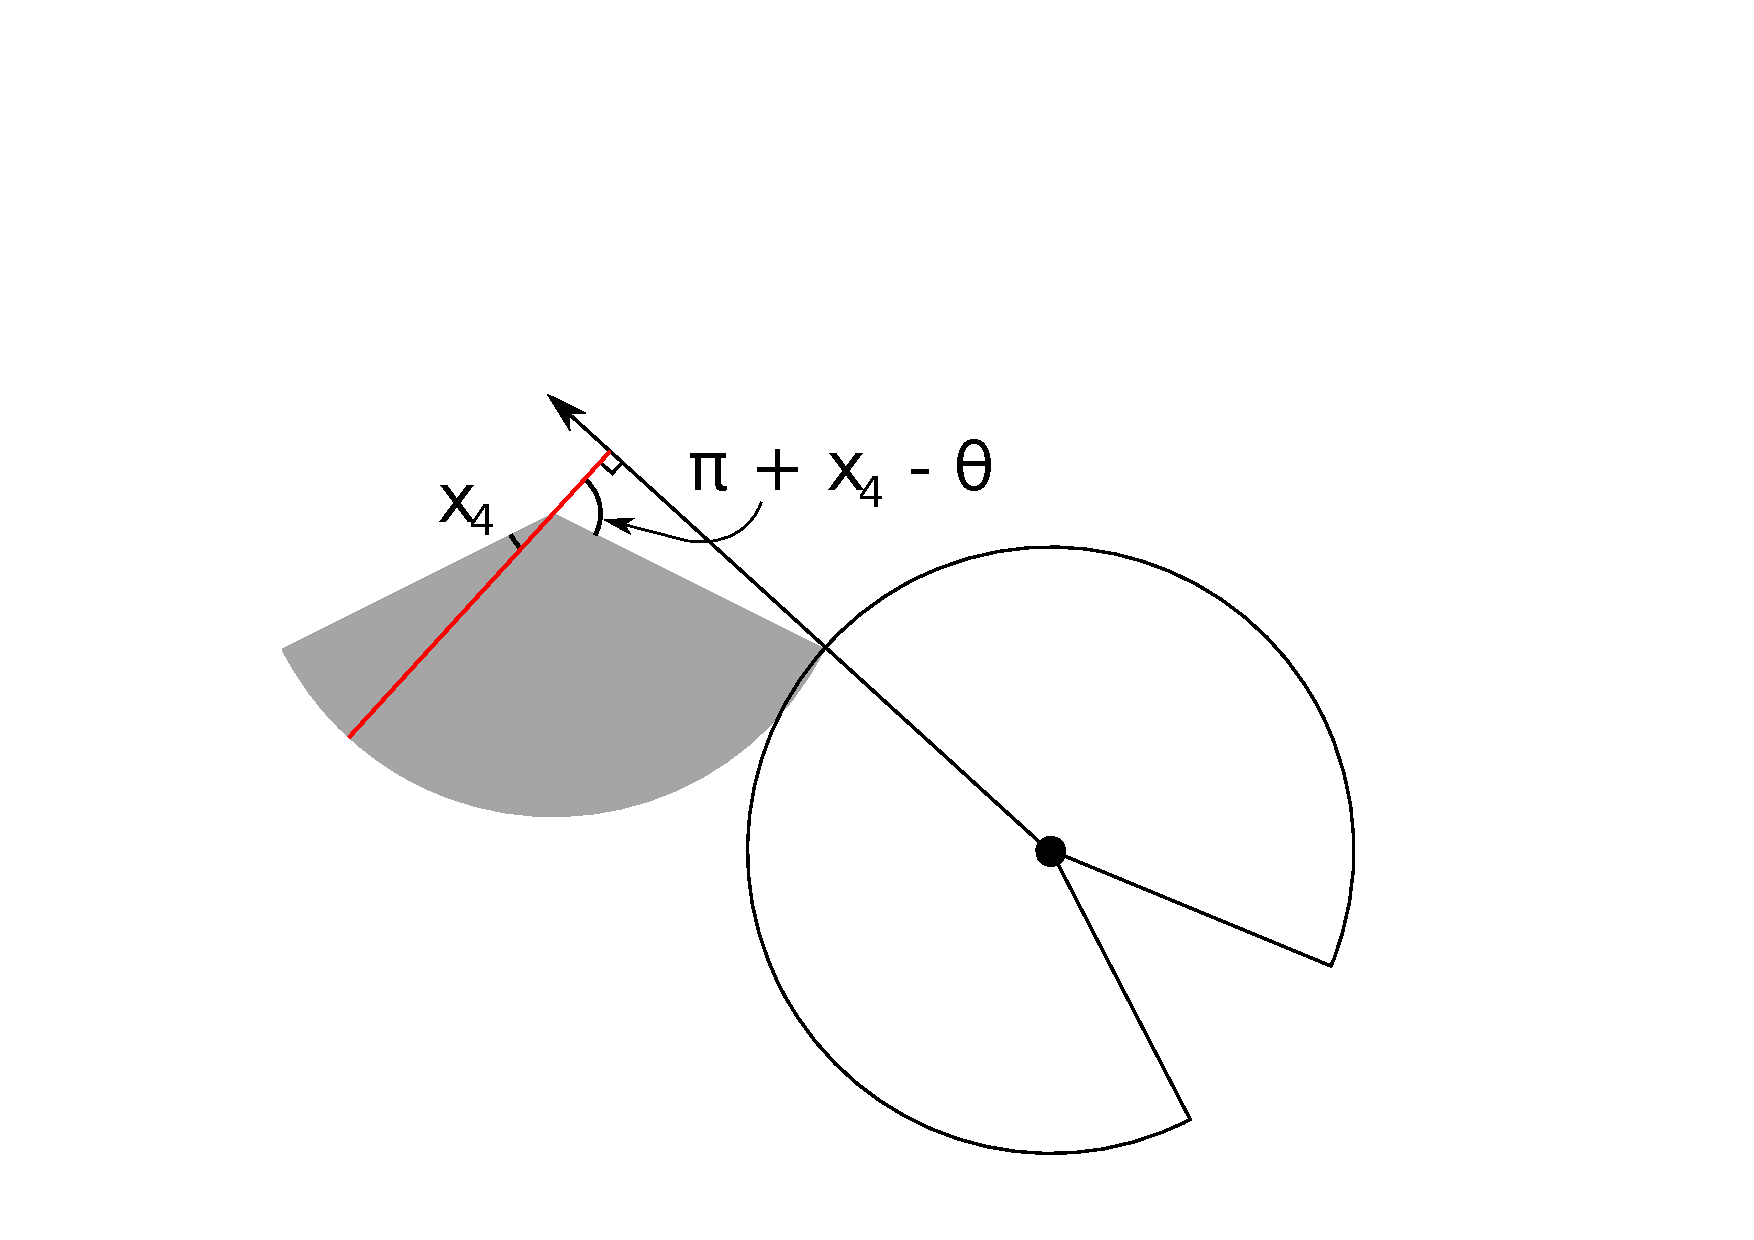
\includegraphics[width=0.5\textwidth, trim=5cm 1cm 4cm 1cm]{imgs/nw2.pdf}
  }
  \subfloat[\label{fig:NW1behindFull}]{
    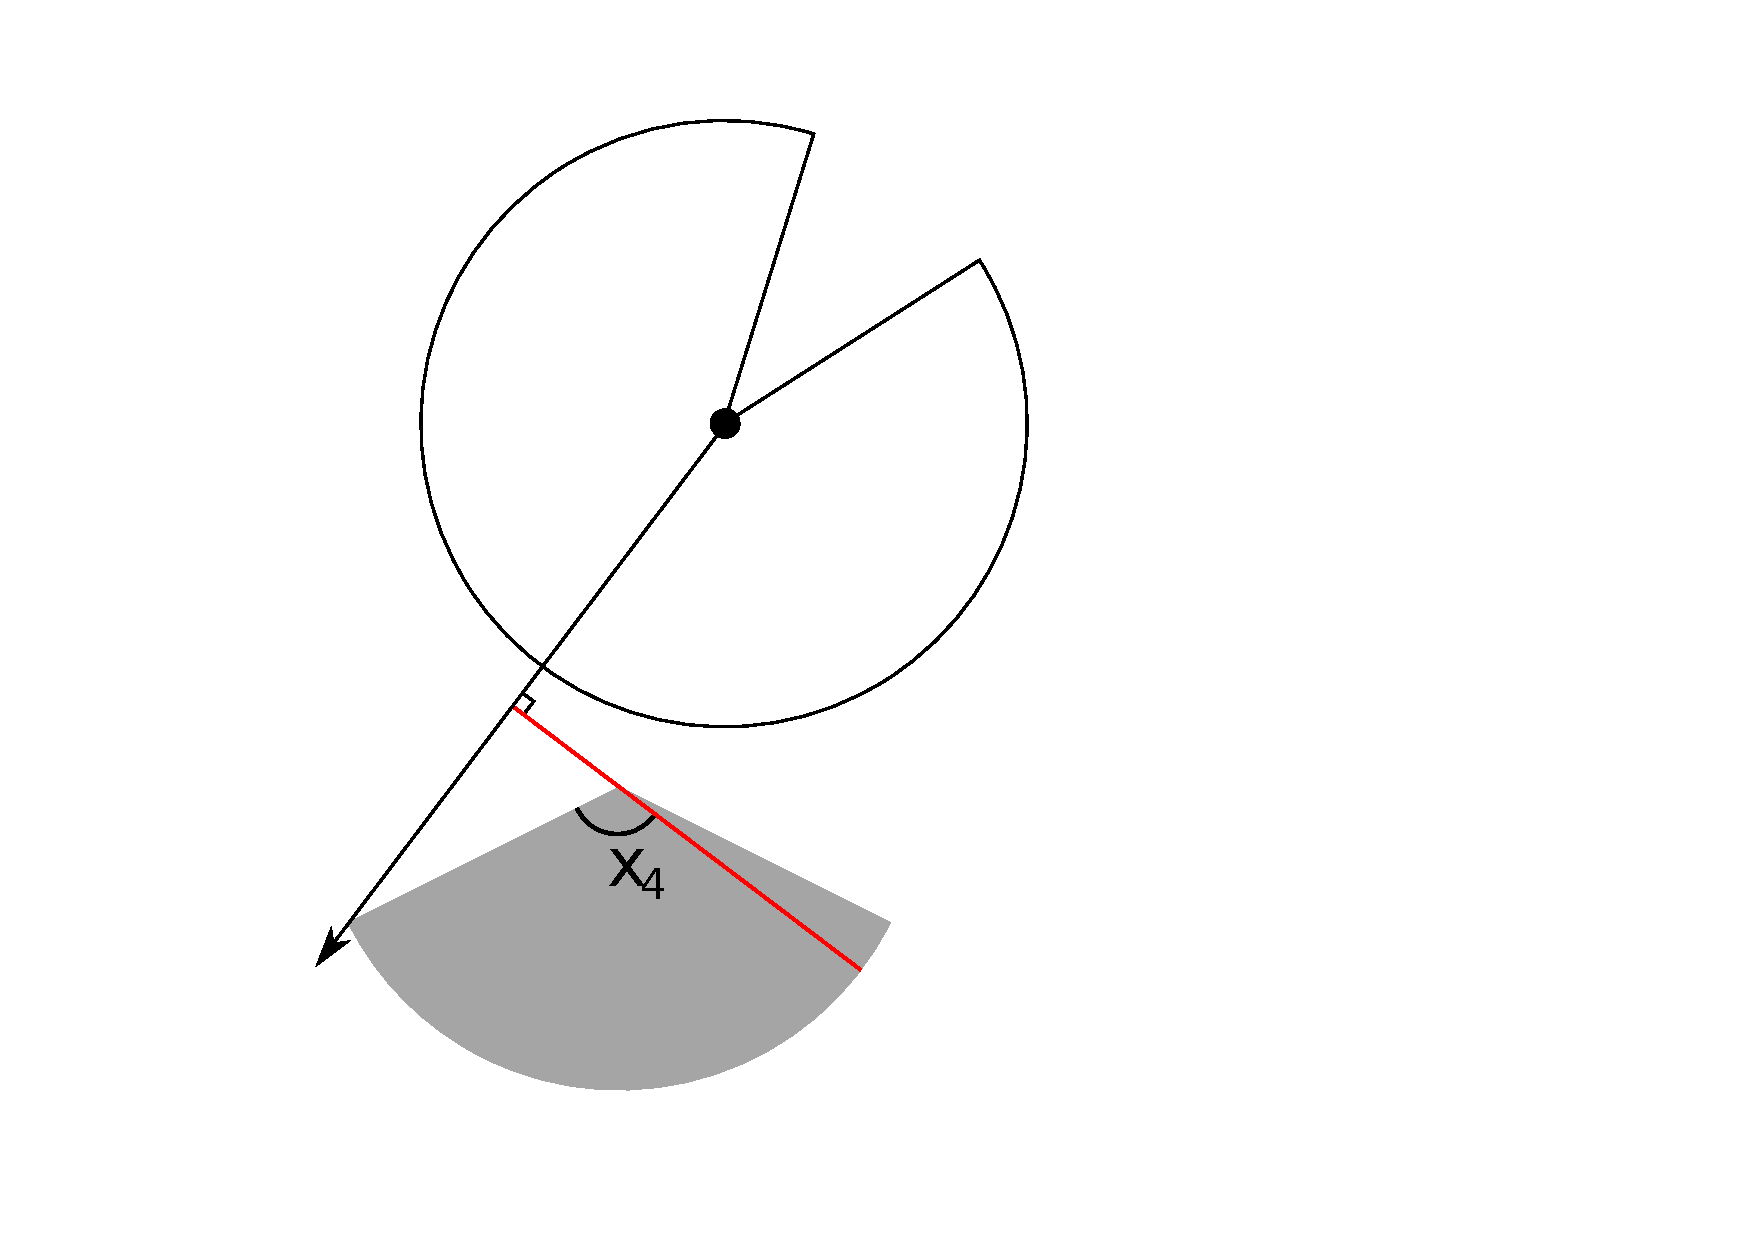
\includegraphics[width=0.5\textwidth, trim=0cm 1cm 4cm 1cm]{imgs/nw4.pdf}
  }
}
\caption[The second and fourth profiles of NW1]{
The second and fourth profiles of NW1.
The left side of of both profiles is of width $r$ while the right side differs.
(a) The right side of the profile is $r\cos(\pi+x_4-\theta) = - r\cos(\theta - x_4 )$ 
(b) The right side is $r\cos(\pi-x_4) = - r\cos x_4$ respectively.
In both images the sector shaped detection region is shown in grey.
Animals are filled black circles and the animal signal is an unfilled sector.
The animals direction of movement is indicated with an arrow.
The profile $p$ is shown with a red line.
}
\label{fig:NW1}
\end{figure}

\subsection{Model NW1} \label{NW1}

NW1 is the first model with $\theta < \pi$.
Whereas previously the focal angle has always been $x_1$, we now use different focal angles.
$x_2$ and $x_3$ correspond to $\gamma_1$ and $\gamma_2$ in \cite{rowcliffe2008estimating} while $x_4$ is new.
They are described in Figure~\ref{fig:xis}b--d.

There are five different profiles in NW1.
\begin{enumerate}
\item $x_2$ has an interval of $[\pi/2, \theta/2]$ which is from the angle of approach being directly towards the sensor until the profile is parallel to the left hand radius of the sensor sector (Figure~\ref{fig:x2}).
During this interval the profile width is $2r\sin\left(\theta/2\right)\sin(x_2)$ which is calculated using the equation for the length of a chord .
Note that while rotating anti-clockwise (as usual) $x_2$ decreases in size.
\item From here, we examine focal angle $x_4$ (note that $x_3$ is used in later models, but is not relevant here).  The left side of the profile is a full radius while the right side is limited to $- r\cos(x_4 - \theta)$ (Figure~\ref{fig:NW1AT}).
\item At $x_4 =  \theta - \pi/2$, the profile is perpendicular to the edge of the sensor area.
Here, the right side of the profile is $0r$ giving a profile size of $r$.
  %@tim is left side r?
\item When $x_4 = \pi/2$ the angle of approach is from behind the sensor, but we can once again be detected on the right side of the sensor (Figure~\ref{fig:NW1behindFull}).
Therefore the width of the profile is $r - r\cos(x_4)$.
\item  Finally, we have the $x_2$ profile, but from behind.
\end{enumerate}



\input{latexFiles/pNW1.tex}

\subsection{Models NW2--4} \label{NW2--4}
% @tim this is still crap
The models NW2--4 have the five potential profiles in NW1 but not all profiles occur in each model, and the angle at which transitions occur are different.
Furthermore, there is one extra profile possible.
\begin{enumerate}
\item When approaching the sensor from behind, there is a period where the profile is $r$ wide as in NW1 profile (3).
\item At some point after profile (1) animals to the right of the sensor can be detected again.
If this occurs in the $x_4$ region, the profile width becomes  $r - r\cos(x_4)$ as in NW1.
\item However, as $\alpha$ is now less than $2\pi$, animals to the right of the sensor may be undetectable until we are in the second $x_2$ region.
In this case, when we first enter the second $x_2$ region, the profile has a width of $r\cos(x_2 - \theta/2)$.
This occurs only if $\alpha \le 3\pi - 2\theta$.
This inequality is found by noting that animals to the right of the sensor can be detected again at $x_4 = 3\pi/2 - \alpha$ but the $x_2$ region starts at $x_4 = \theta$.
The new profile in $x_2$ will only occur if  $ \theta < 3\pi/2 - \alpha/2$ which is rearranged to find the inequality above.
This defines the boundary between NW2 and NW3.
\item As $\alpha \le 2\pi$ it is possible that when the angle of approach is from directly behind the sensor the animal will not be detected at all.
This is the case if $\alpha/2\le \pi-\theta/2$ (Figure~\ref{fig:NW2--4}).
This inequality (simplified as $\alpha\le 2\pi-\theta$) defines the boundary between NW3 and NW4.
\end{enumerate}



\begin{figure}[t]
  \centering
{
  \subfloat[\label{fig:NW2--4behind}]{
    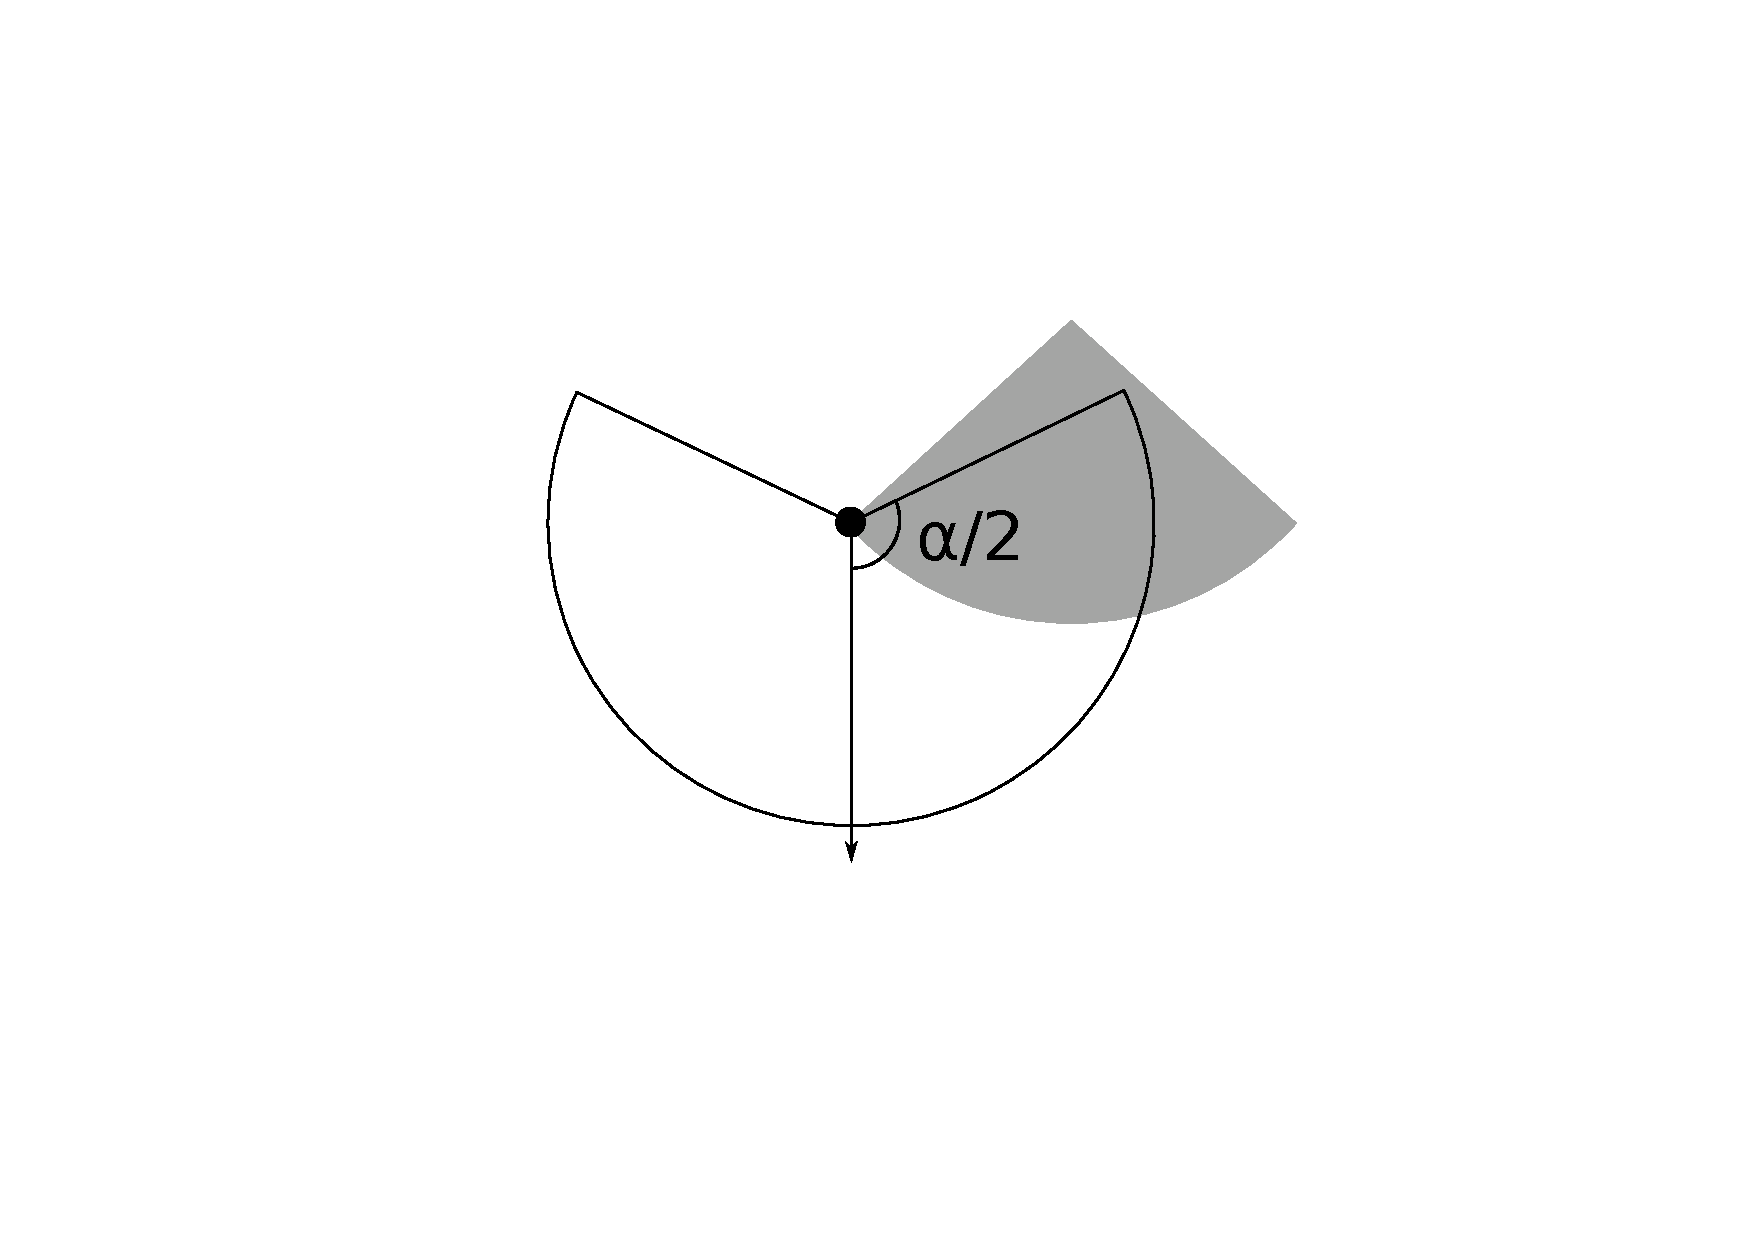
\includegraphics[width=0.45\textwidth, trim=5cm 6cm 4cm 1cm]{imgs/behind.pdf}   
  }
  \subfloat[\label{fig:NW2--4behind2}]{
    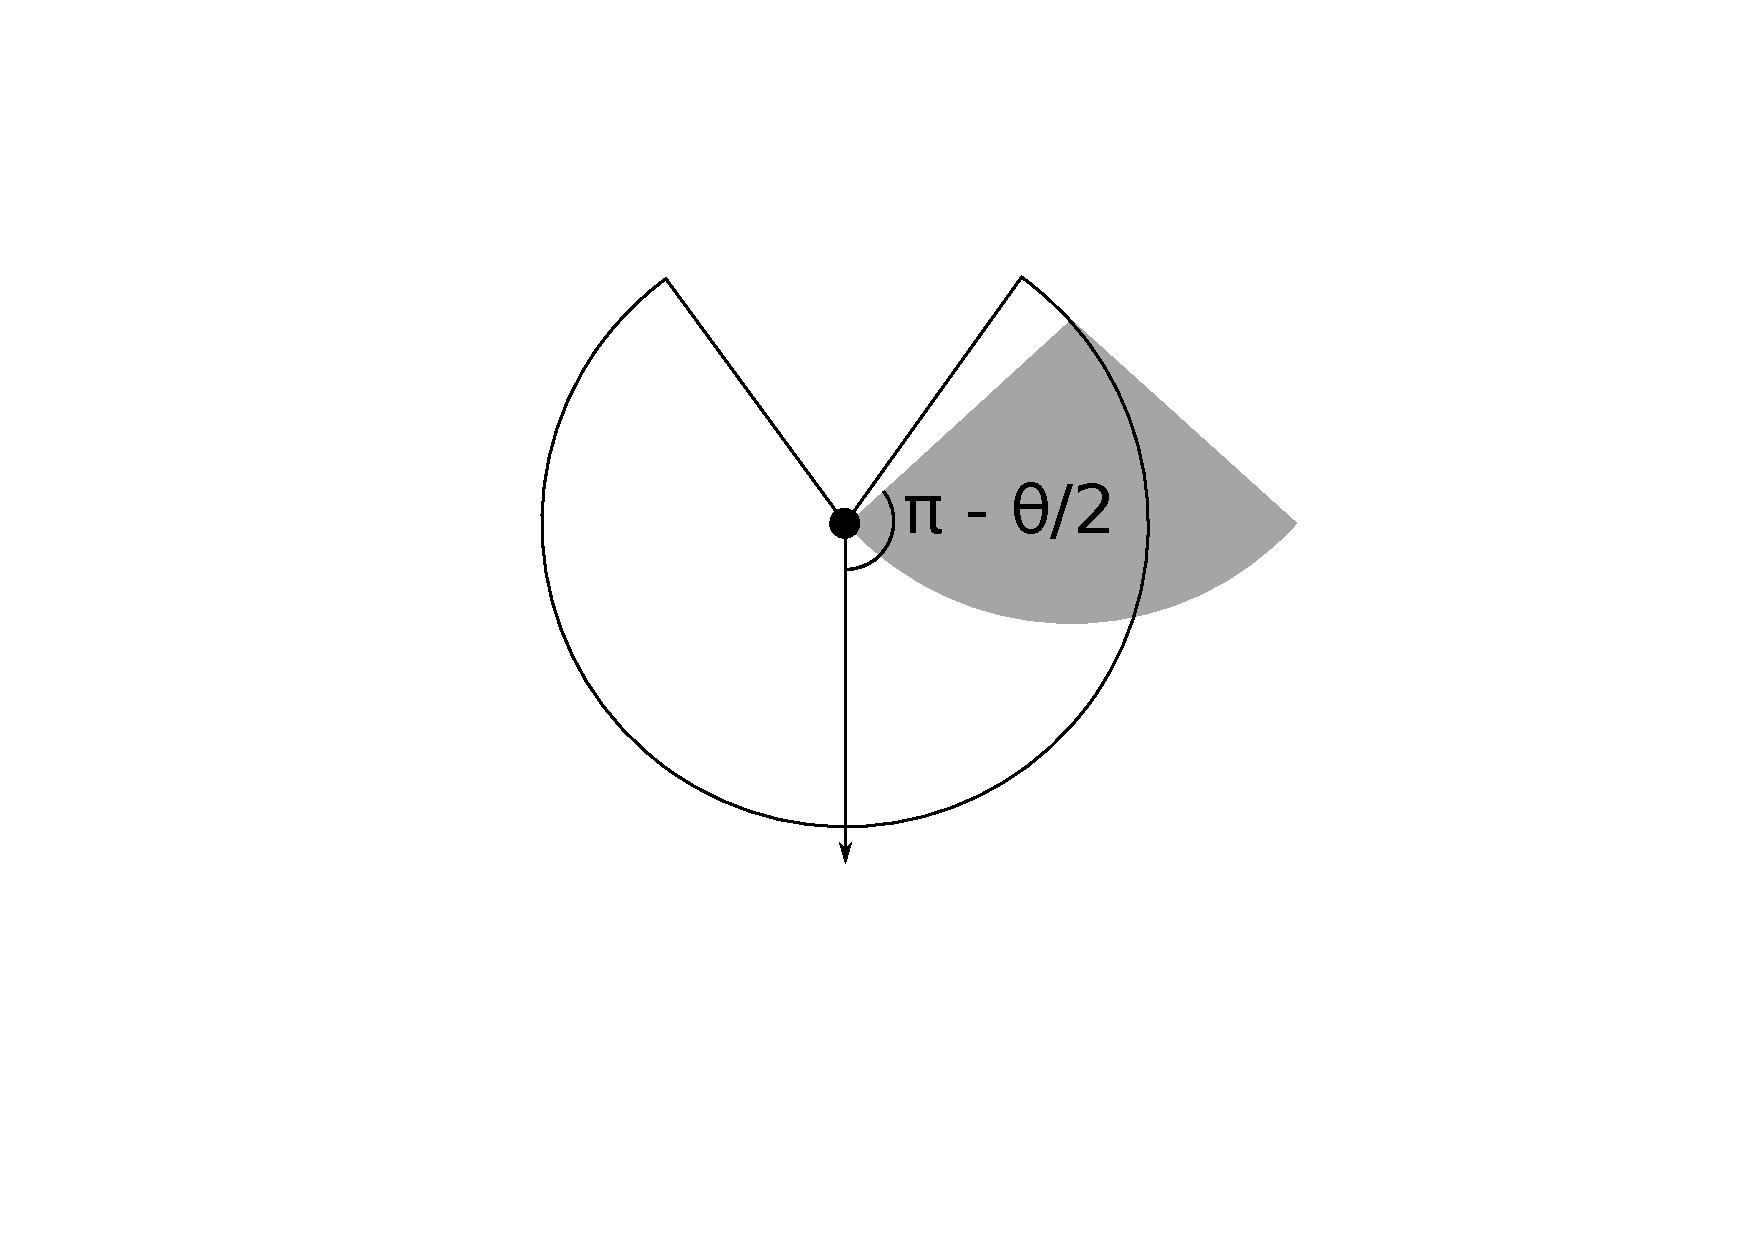
\includegraphics[width=0.45\textwidth, trim=5cm 6cm 4cm 1cm]{imgs/behind2.pdf}      
  }
}
\caption[Profile sizes for an animal approaching from behind: models NW2--4]{
Profile sizes when an animal approaches from behind in models NW2--4.
If $\alpha$ is relatively large, animals can be detected when approaching from behind.
Otherwise animals cannot be detected.
The sector shaped detection region is shown in grey.
Animals are filled black circles and the animal signal is an unfilled sector.
The animals direction of movement is indicated with an arrow.
(a) If $\alpha/2$ is less than $\pi - \theta/2$, as is the case here, then the width of the profile when an animal approaches directly from behind is zero.
(b) If $\alpha/2 > \pi - \theta/2$ the profile width from behind is $2r\sin\left(\theta/2\right)\sin(x_2)$.
}
\label{fig:NW2--4}
\end{figure}


\subsubsection{Model NW2} \label{NW2}

NW2 is bounded by $\alpha \ge 3\pi - 2\theta$, $\alpha \le 2\pi$ and $\theta\le\pi$ (Figure~\ref{fig:equalRegions}).

NW2 has all five profiles as found in NW1.
However, the change from the $r$ profile (third integral) to the $r - r\cos(x_4)$ profile (fourth integral) occurs at $x_4 = 3\pi/2 - \alpha/2$ instead of at $x_4 = \theta$.

\input{latexFiles/pNW2.tex}


\subsubsection{Model NW3} \label{NW3}

NW3 is bounded by $\alpha \le 3\pi - 2\theta$, $\alpha\ge 2\pi-\theta$ and $\theta\ge\pi/2$ (Figure~\ref{fig:equalRegions}).

NW3 does not have the fourth integral from NW2 as animals are not detectable to the right of the sensor until after the $x_4$ region has ended and the $x_2$ region has begun.
Therefore the second $x_4$ integral has an upper limit of $\theta $ and the profile after has a width of $r\cos(x_2 - \theta/2)$ and is integrated with respect to $x_2$.
The final integral starts at $x_4 = 3\pi/2 - \alpha/2 - \theta/2$ and has the full width of $2r\sin(x_2)\sin(\theta/2)$.

\input{latexFiles/pNW3.tex}

\subsubsection{Model NW4} \label{NW4}

Finally, NW4 is bounded by $\alpha\ge \pi$, $\theta\ge \pi/2$ and $\alpha \le 2\pi - \theta$ (Figure~\ref{fig:equalRegions}).
NW4 is the same as NW3 except that the final profile width is zero and this profile is reached at $\alpha/2+\theta/2-\pi/2$.

\input{latexFiles/pNW4.tex}


\subsection{Model REM} \label{REM}

REM is the model from \cite{rowcliffe2008estimating}.
It has $\alpha =2\pi$ and $\theta \le \pi/2$ (Figure~\ref{fig:equalRegions}).
It has three profile widths, two of which are repeated, once as the animal approaches from in front of the sensor and once as the animal approaches from behind the sensor.

\begin{enumerate}
\item Starting with an approach direction of directly towards the sensor, and examining focal angle $x_2$, the profile width is $2r\sin(x_2)\sin(\theta/2)$.
\item When the profile is perpendicular to the radius on the right hand of the sector sensor region, we instead examine $x_3$ where the profile width is $r\sin(x_3)$.
\item At $x_3=\pi/2$ the profile becomes simply $r$ and this continues for $\theta $ radians of $x_4$.
\item The $x_3$ profile is then repeated with an approach direction from behind the sensor.
\item Finally the $x_2$ profile is repeated, again with an approach direction from behind the sensor.
\end{enumerate}

\input{latexFiles/pREM.tex}

\subsection{Models NW5--7} \label{NW57}

In the models NW5--7, the sensor has $\theta \le \pi/2$ as in the REM.
As $\alpha \ge \pi$ a lot of the profiles are similar to the REM.
Specifically, the first three profiles are always the same as the first three profiles of the REM.
This is because when an animal is moving towards the sensor, the $\alpha \ge \pi$ signal is no different to a $2\pi$ signal.
However, when approaching the sensor from behind, things are slightly different.
The animal can only be detected by the sensor if the signal width is large enough that it can be detected once it has passed the sensor.
                    
\begin{enumerate}
\item Starting with an approach direction of directly towards the sensor, and examining focal angle $x_2$, the profile width is $2r\sin(x_2)\sin(\theta/2)$.
\item When the profile is perpendicular to the radius edge of the sector sensor region, we instead examine $x_3$ where the profile width is $r\sin(x_3)$.
\item At $x_3=\pi/2$ the profile becomes simply $r$ and this continues for $\theta $ radians of $x_4$.
\item If $\alpha \le 2\pi + 2\theta$, the animal becomes undetectable during this profile when  $x_3$ has decreased in size to $\pi - \alpha/2$.
This inequality marks the boundary between NW7 and NW6.
\item If instead $\alpha \ge 2\pi + 2\theta$ then the animal does not become undetectable during the $x_3$ focal angle.
Instead the profile has width greater than zero for the whole of the $x_3$ angle.
The $x_2$ profile starts with width $r\cos(x_2 - \theta/2)$ as only animals approaching to the left of the sensor are detectable.
\item During this second $x_2$ profile the signal width needed for animals to be detected to the left of the detector is increasing while the angle needed for animals to be detected to the right of the detector is decreasing.
Therefore, either the left side becomes undetectable, making both sides undetectable (this occurs if $\alpha \le 2\pi - \theta$ as in NW6) \item or the right becomes detectable (if $\alpha \ge 2\pi - \theta$ as in NW5), making both sides detectable and giving a profile width of $2r\sin(x_2)\sin(\theta/2)$.
\end{enumerate}


\subsubsection{Model NW5} \label{NW5}

NW5 is bounded by $\alpha \ge 2\pi - \theta$, $\alpha \le 2\pi$ and $\theta \le \pi/2$ (Figure~\ref{fig:equalRegions}).

It is the same as REM except that it includes the extra profile in $x_2$ (the fifth integral) where only animals approaching to the left of the profile are detected.

\input{latexFiles/pNW5.tex}

\subsubsection{Model NW6} \label{NW6}

NW6 is bounded by $\alpha \le 2\pi - \theta$, $\alpha \ge 2\pi + 2\theta$ and $\theta \le \pi/2$ (Figure~\ref{fig:equalRegions}).

NW6 is the same NW5 except that as $\alpha \le 2\pi - \theta$, animals that approach from directly behind the detector are not detected.
Therefore at $x_2 = \alpha/2 + \theta/2 - \pi/2$ the profile width goes to zero and therefore the last integral in NW5 is not included.

\input{latexFiles/pNW6.tex}



\subsubsection{Model NW7} \label{NW7}

NW7 is bounded by $\alpha \ge 2\pi + 2\theta$, $\alpha \ge \pi$ and $\theta \ge 0$ (Figure~\ref{fig:equalRegions}).

It is similar to NW6 but does not include the last integral as during the $x_3$ profile, at $x_3 = \pi - \alpha/2$ the signal width is too small for any animals to be detected, so the profile width goes to zero.

\input{latexFiles/pNW7.tex}





\subsection{Model SW1--3} \label{SW13}
 
The models in SW1--3 are described with the two focal angles used in models NW2--4, $x_2$ and $x_4$.
As $\alpha \le\pi$ an animal can never be detected if it is approaching the detector from behind.
This makes these models simpler in that they go through the $x_2$ and $x_4$ profiles only once each.

\begin{figure}[t]
  \centering
{
  \subfloat[\label{fig:SWforward}]{
    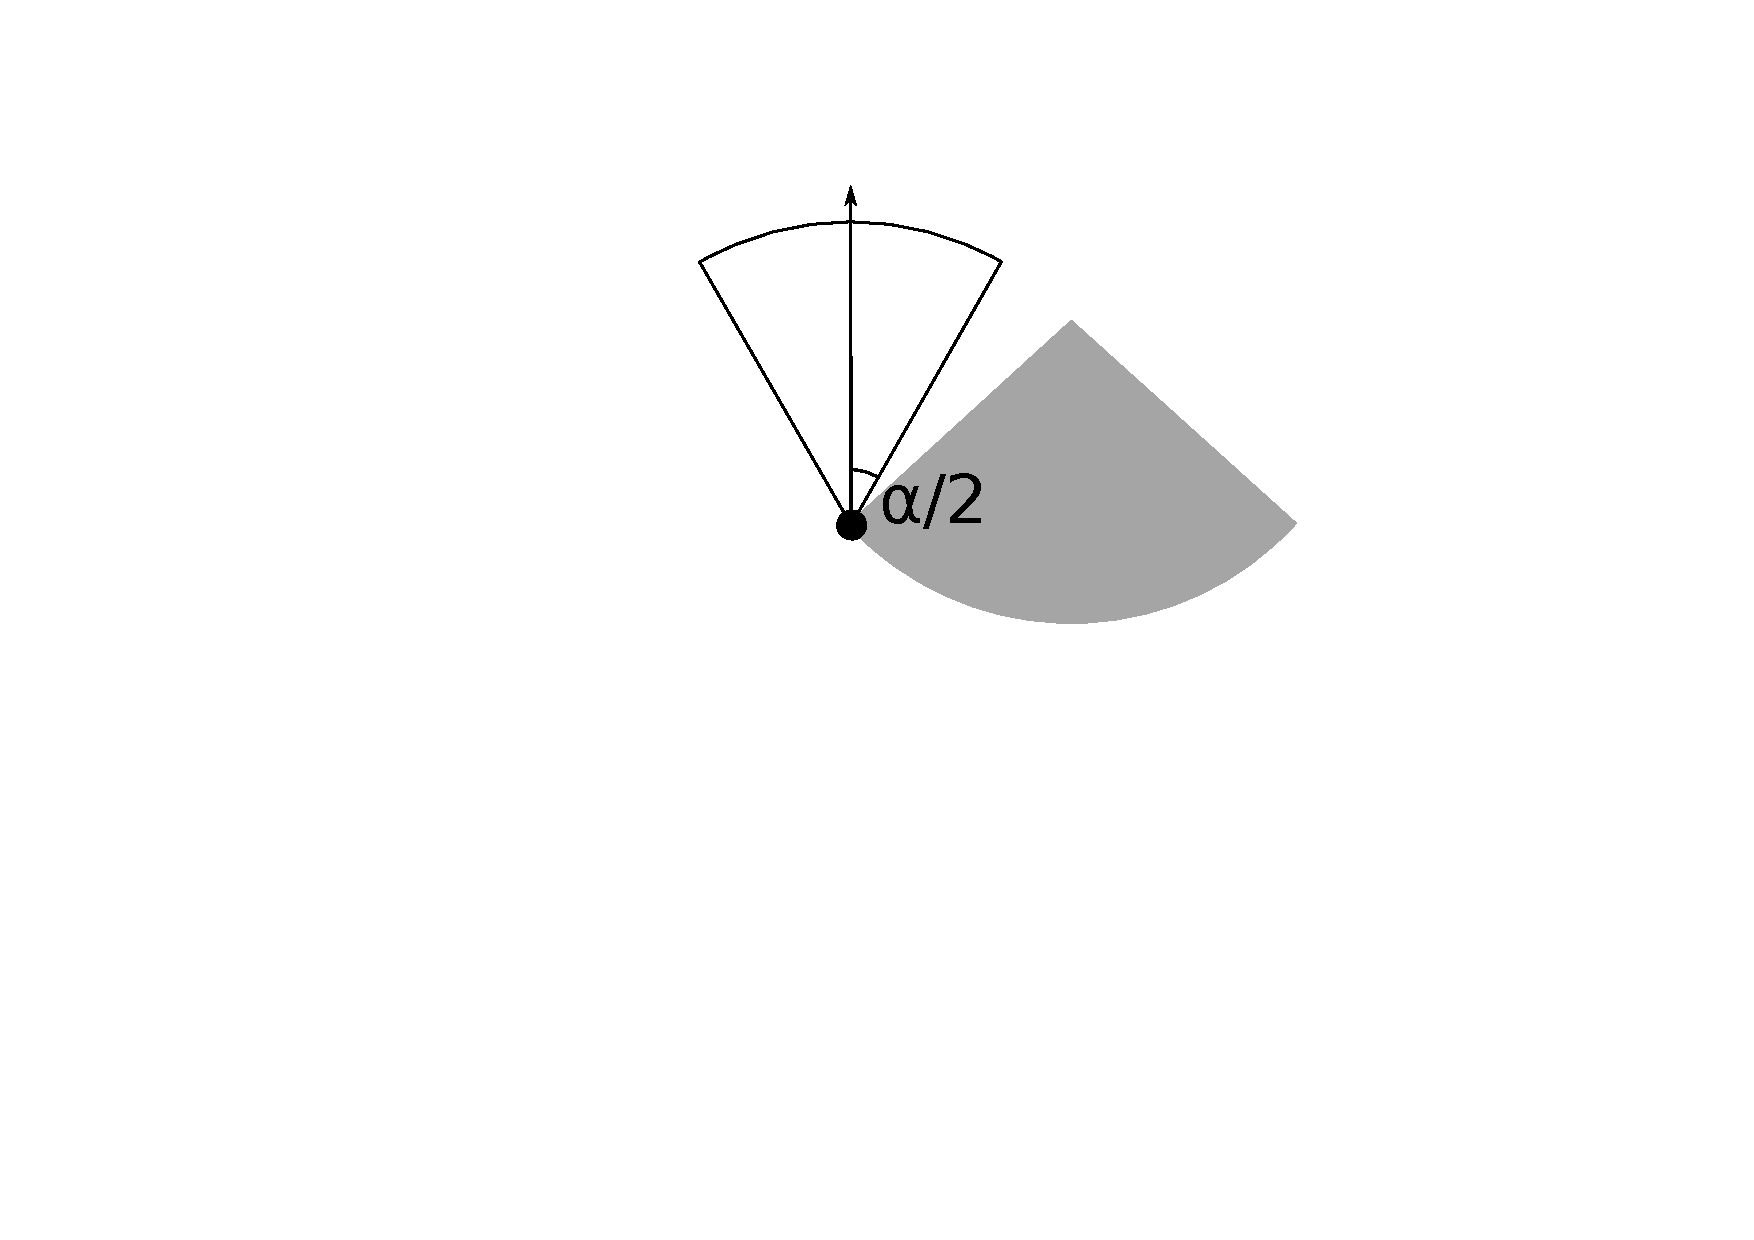
\includegraphics[width=0.45\textwidth, trim=7cm 10cm 6cm 1cm]{imgs/forward.pdf}
  }
  \subfloat[\label{fig:SWforwad2}]{
    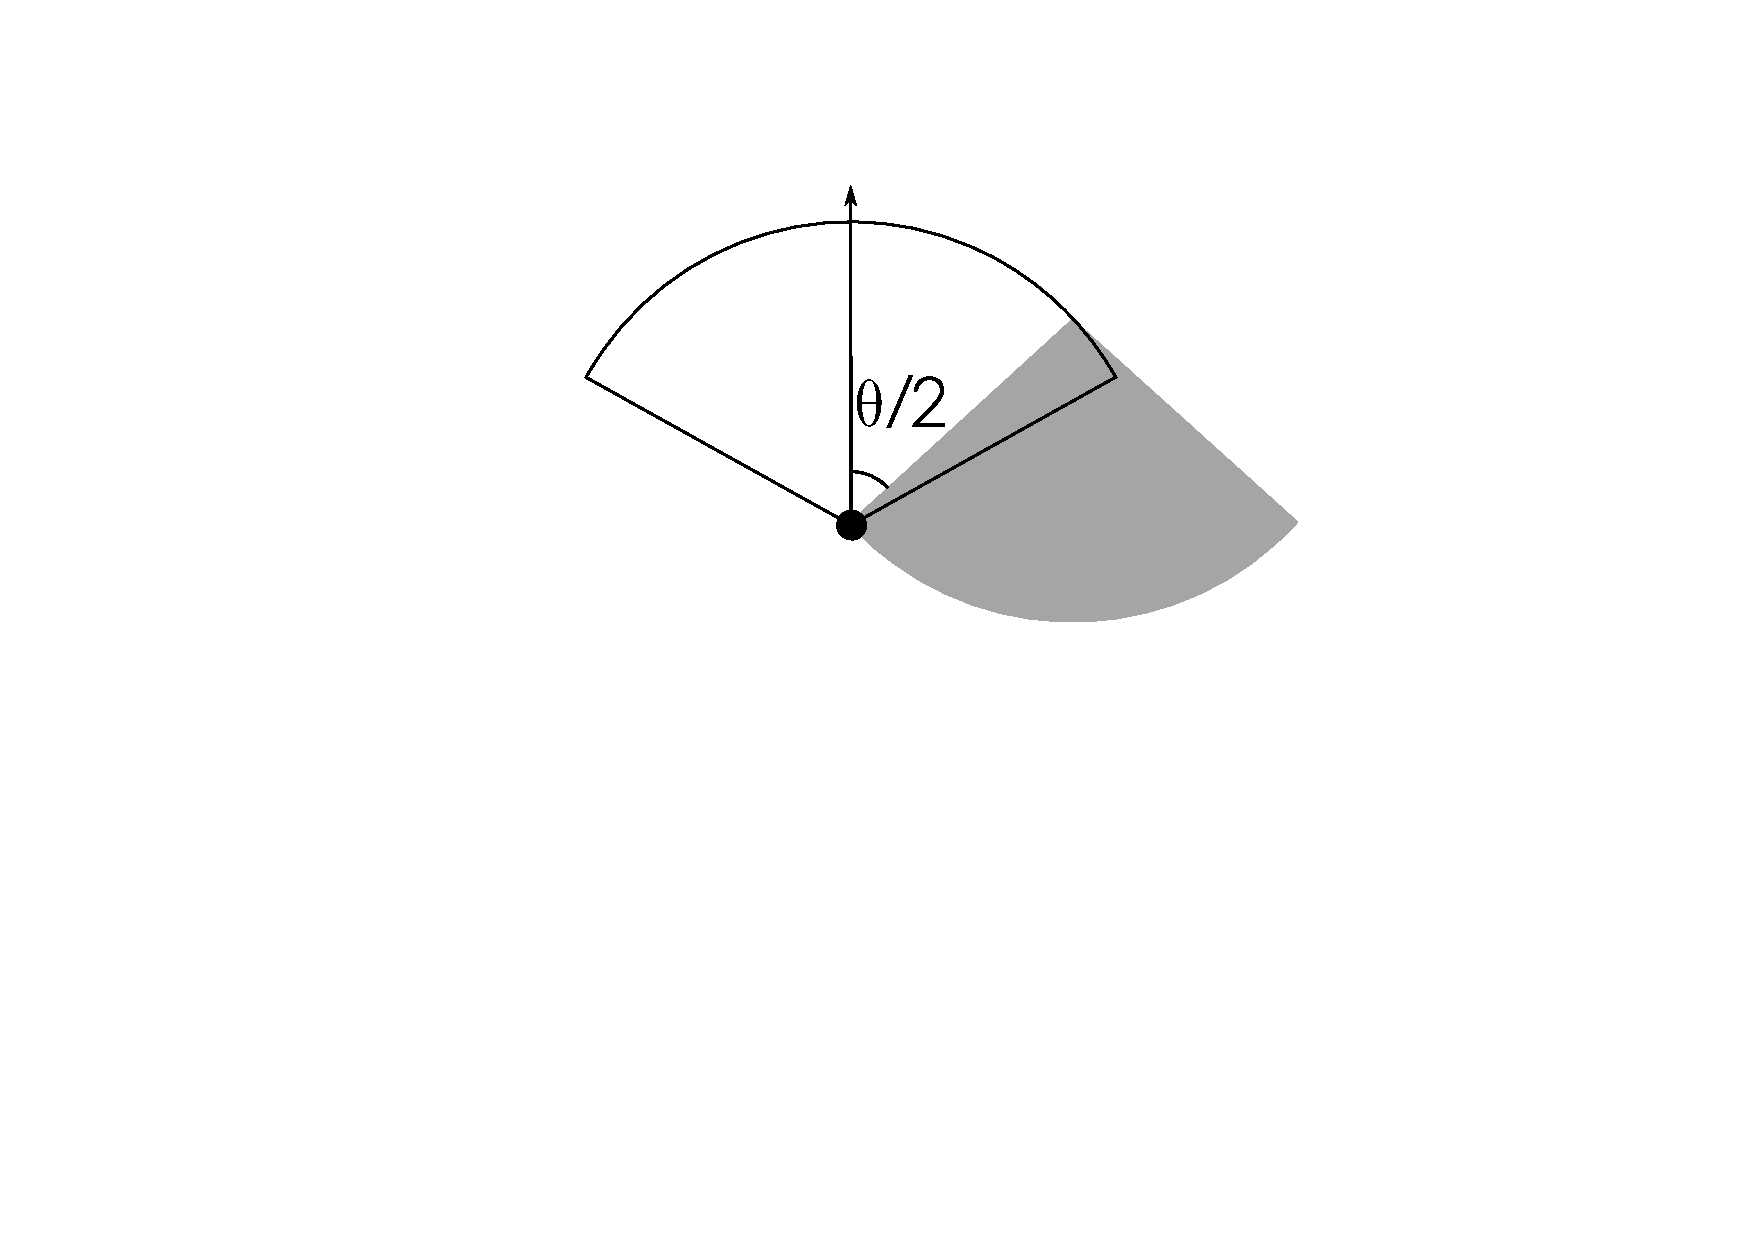
\includegraphics[width=0.45\textwidth, trim=7cm 10cm 6cm 1cm]{imgs/forward2.pdf}
  }
}
\caption[The first profile in SW models]{
The first profile in SW models is limited by either $\alpha$ or $\beta$ depending on whether $\alpha < \beta$.
The sector shaped detection region is shown in grey.
Animals are filled black circles and the animal signal is an unfilled sector.
The animals direction of movement is indicated with an arrow.
(a)  As $\alpha/2 < \theta/2$ the profile width is limited by the signal width rather than the sensor region.
The profile width is $2r\sin\left(\alpha/2\right)$ (b) As $\alpha/2 > \theta/2$ the profile width is limited by the sensor region, not the signal width.
The profile width is $2r\sin\left(\theta/2\right)\sin(x_2)$.
}
\label{fig:forward}
\end{figure}


There are five potential profile sizes.
\begin{enumerate}
\item At the beginning of $x_2$, with an approach direction directly towards the sensor, the parameter that limits the width of the profile can either be the sensor width,  in which case the profile width is $2r\sin\left(\theta/2\right)\sin(x_2)$.
\item Or the signal width can be the limiting parameter, in which case the profile width is instead $2r\sin(\alpha /2)$ (Figure~\ref{fig:forward})
\item The next potential profile in $x_2$ has a width of $r\sin(\alpha/2) - r\cos(x_2 + \theta/2)$ as the right side of the profile is limited by the width of the sensor region while the left side is limited by the signal width.
However, the angle at which the profile starts depends on whether the first profile was 1) or 2) above.
If the first profile is profile 1) then the profile is limited on both sides by the sensor region and then the left side of the profile becomes limited by the signal width.
This happens at $x_2 = \pi/2 - \alpha/2 + \theta/2$.
If however the first profile was 2) then the first profile is limited by the signal width.
We move into the new profile when the right side of the profile becomes limited by the sensor region.
This occurs at $x_2 = \pi/2 + \alpha/2 - \theta/2$.


\item In the $x_4$ region the left side of the profile is always $r\sin(\alpha /2)$ while the right side is either 0, giving a profile of $r\sin(\alpha /2)$.

\item Or limited by the sensor giving a profile of size $r\sin (\alpha /2) -r\cos(x_4-\theta) $.
\end{enumerate}

\subsubsection{Model SW1} \label{SW1}

SW1 is bounded by $\alpha \ge \theta$, $\alpha \le\pi$ and $\theta \le \pi$ (Figure~\ref{fig:equalRegions}).

As $\alpha $ is large the first profile is limited by the size of the sensor region giving it a width of $2r\sin\left(\theta/2\right)\sin(x_2)$.
It is the only one of the three SW models to start in this way.
Later on, still with $x_2$ as the focal angle the left side of the profile does become limited by the signal width.
So at $x_2= \pi/2 - \alpha/2 + \theta/2$ the profile width becomes $r\sin(\alpha/2) - r\cos(x_2 + \theta/2)$.

As we enter the $x_4$ region, the profile remains limited by the signal on the left and by the sensor on the right, giving a profile width of  $r\sin (\alpha /2) -r\cos(x_4-\theta) $.
Finally, at $x_4 = \theta - \pi/2$ the right side of the profile becomes zero and the profile is width is $r\sin(\alpha /2)$.

\input{latexFiles/pSW1.tex}

\subsubsection{Model SW2} \label{SW2}

SW2 is bounded by $\theta \ge \pi/2$, $\alpha \le \theta$ and $\alpha \ge 2\theta -\pi$ (Figure~\ref{fig:equalRegions}).

SW2 is largely similar to SW1.
However, as $\alpha \le \theta$ the first profile is limited by $\alpha$ and not by the detection region.
Therefore the first profile has width $2r\sin(\alpha /2)$.
This also means the transition to the second profile occurs at  $x_2 = \pi/2 + \alpha/2 - \theta/2$ instead of  $x_2 = \pi/2 - \alpha/2 + \theta/2$.

\input{latexFiles/pSW2.tex}



\subsubsection{Model SW3} \label{SW3}

SW3 is bounded by $\alpha \le 2\theta -\pi$ and $\theta \le \pi$ (Figure~\ref{fig:equalRegions}).

SW3 is similar to SW2 except that the profile does not become limited by sensor at all during the the $x_4$ regions.
Therefore, at $x_4 = 0 $ the profile is still of width $2r\sin(\alpha /2)$.
Only at $x_4 = \theta - \pi/2 - \alpha/2$ does the profile become limited on the right by the sensor region.

\input{latexFiles/pSW3.tex}


\subsection{Model SW4--9} \label{SW4--9}

As $\alpha < \pi$, animals approaching the sensor from behind can never be detected, so unlike REM, the second $x_2$ and $x_3$ profiles are always zero.
The six models are split by three inequalities that relate to the models as follows.

\begin{enumerate}
\item Models with $\alpha \le \pi - 2\theta$  have no $x_4$ profile.
This is because at $x_4 = 0$, the signal width is already too small to be detected as can be seen in Figure~\ref{fig:SW4--9nox4} where $\alpha/2 < \pi/2 - \theta$ which simplifies to give the previous inequality.

\item Models with $\alpha \le \theta$ are limited by $\alpha$ in the first, $x_2$ region (Figure~\ref{fig:forward}), rather than being limited by $\theta$.
Therefore this first profile is of width $2r\sin(\alpha/2)$ rather than $2r\sin(\theta/2)\sin(x_2)$.

\item Finally, models with $\alpha \le 2\theta$ have a second profile in $x_2$ where to one side of the sensor $\alpha$ is the limiting factor of profile width, while on the other side $\theta$ is (Figure~\ref{fig:4--9int3}).
This gives a width of $r\sin(\alpha/2) - r\cos(x_2 + \theta/2)$.
This profile does not occur in models with $\alpha \ge 2\theta$.

\end{enumerate}

\begin{figure}[t]
 \centering
{
  \subfloat[\label{fig:SW4--9nox4}]{
    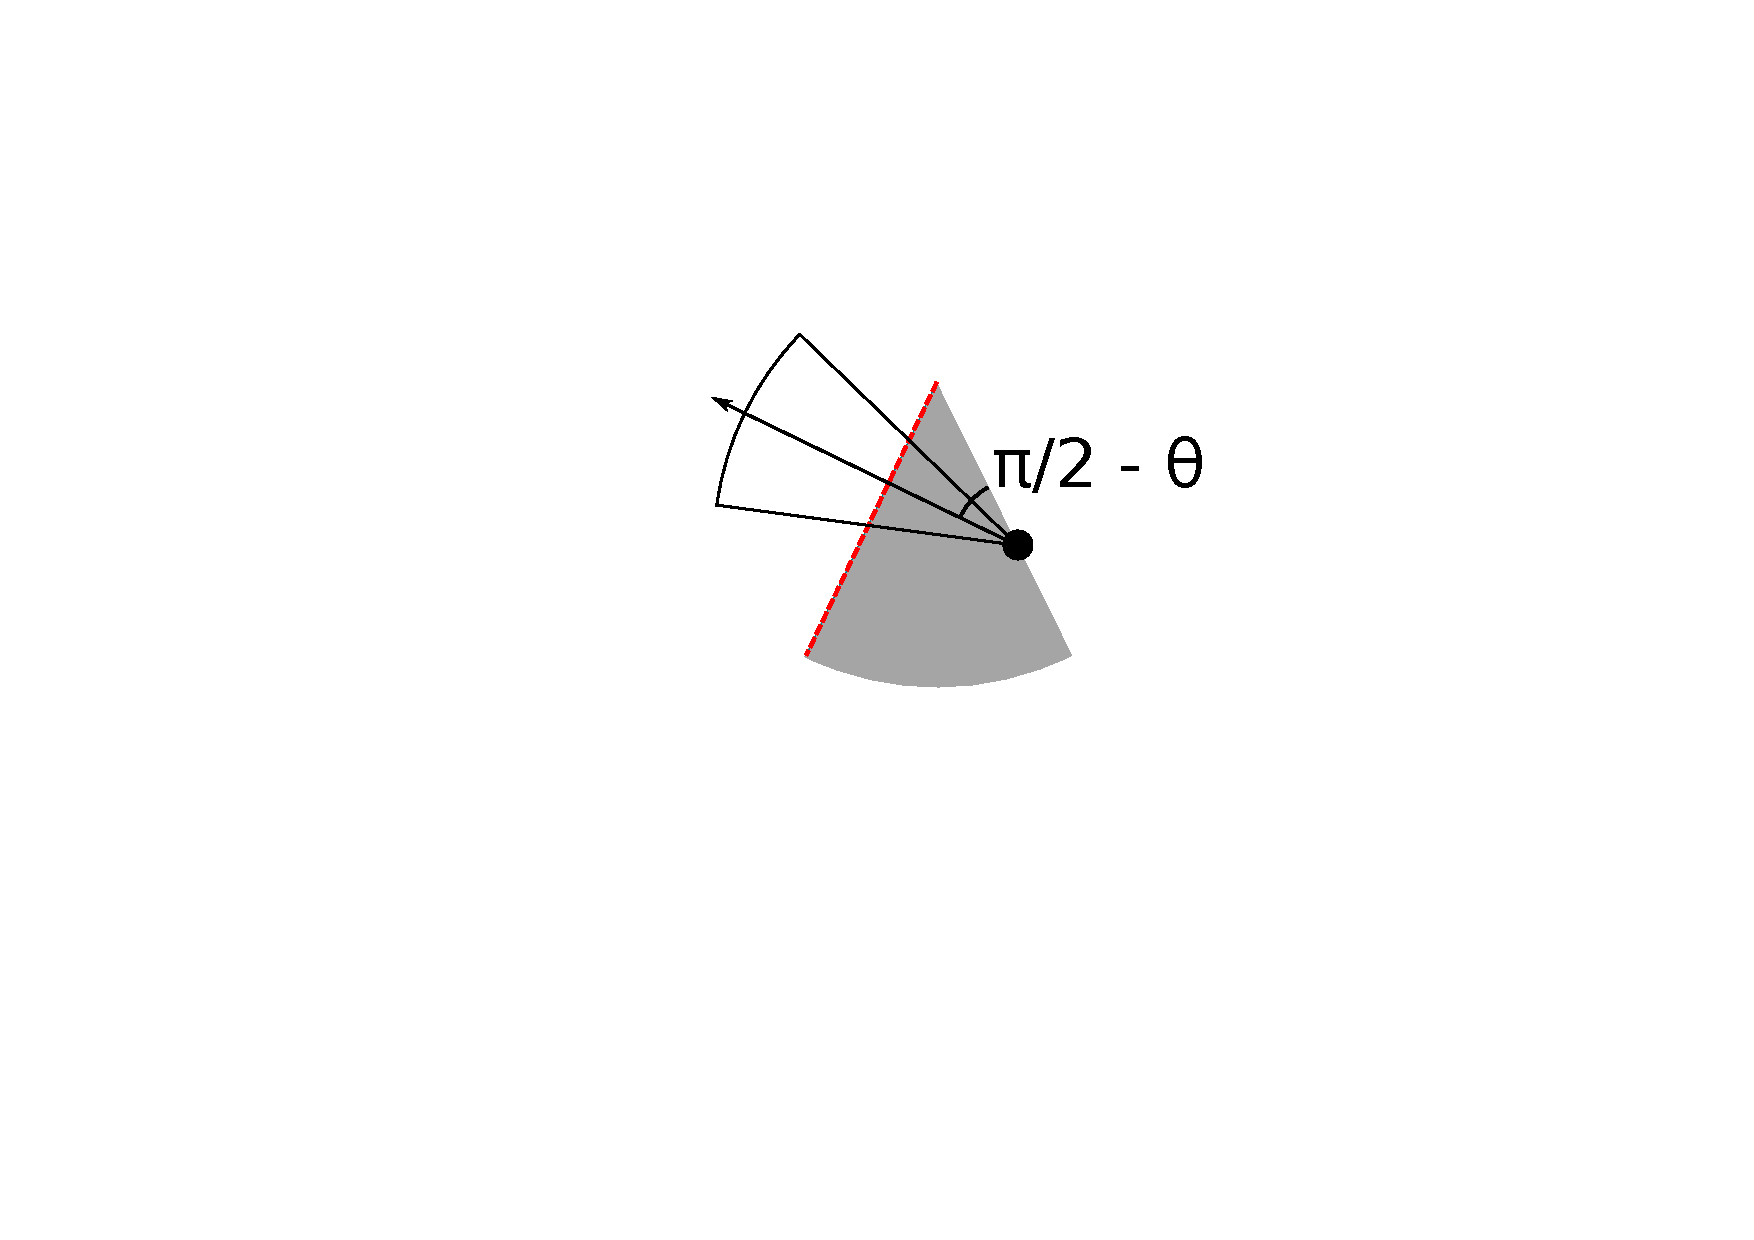
\includegraphics[width=.5\textwidth, trim=8cm 9cm 8cm 4cm]{imgs/x4is0.pdf}
  }
  \subfloat[\label{fig:4--9int3}]{
    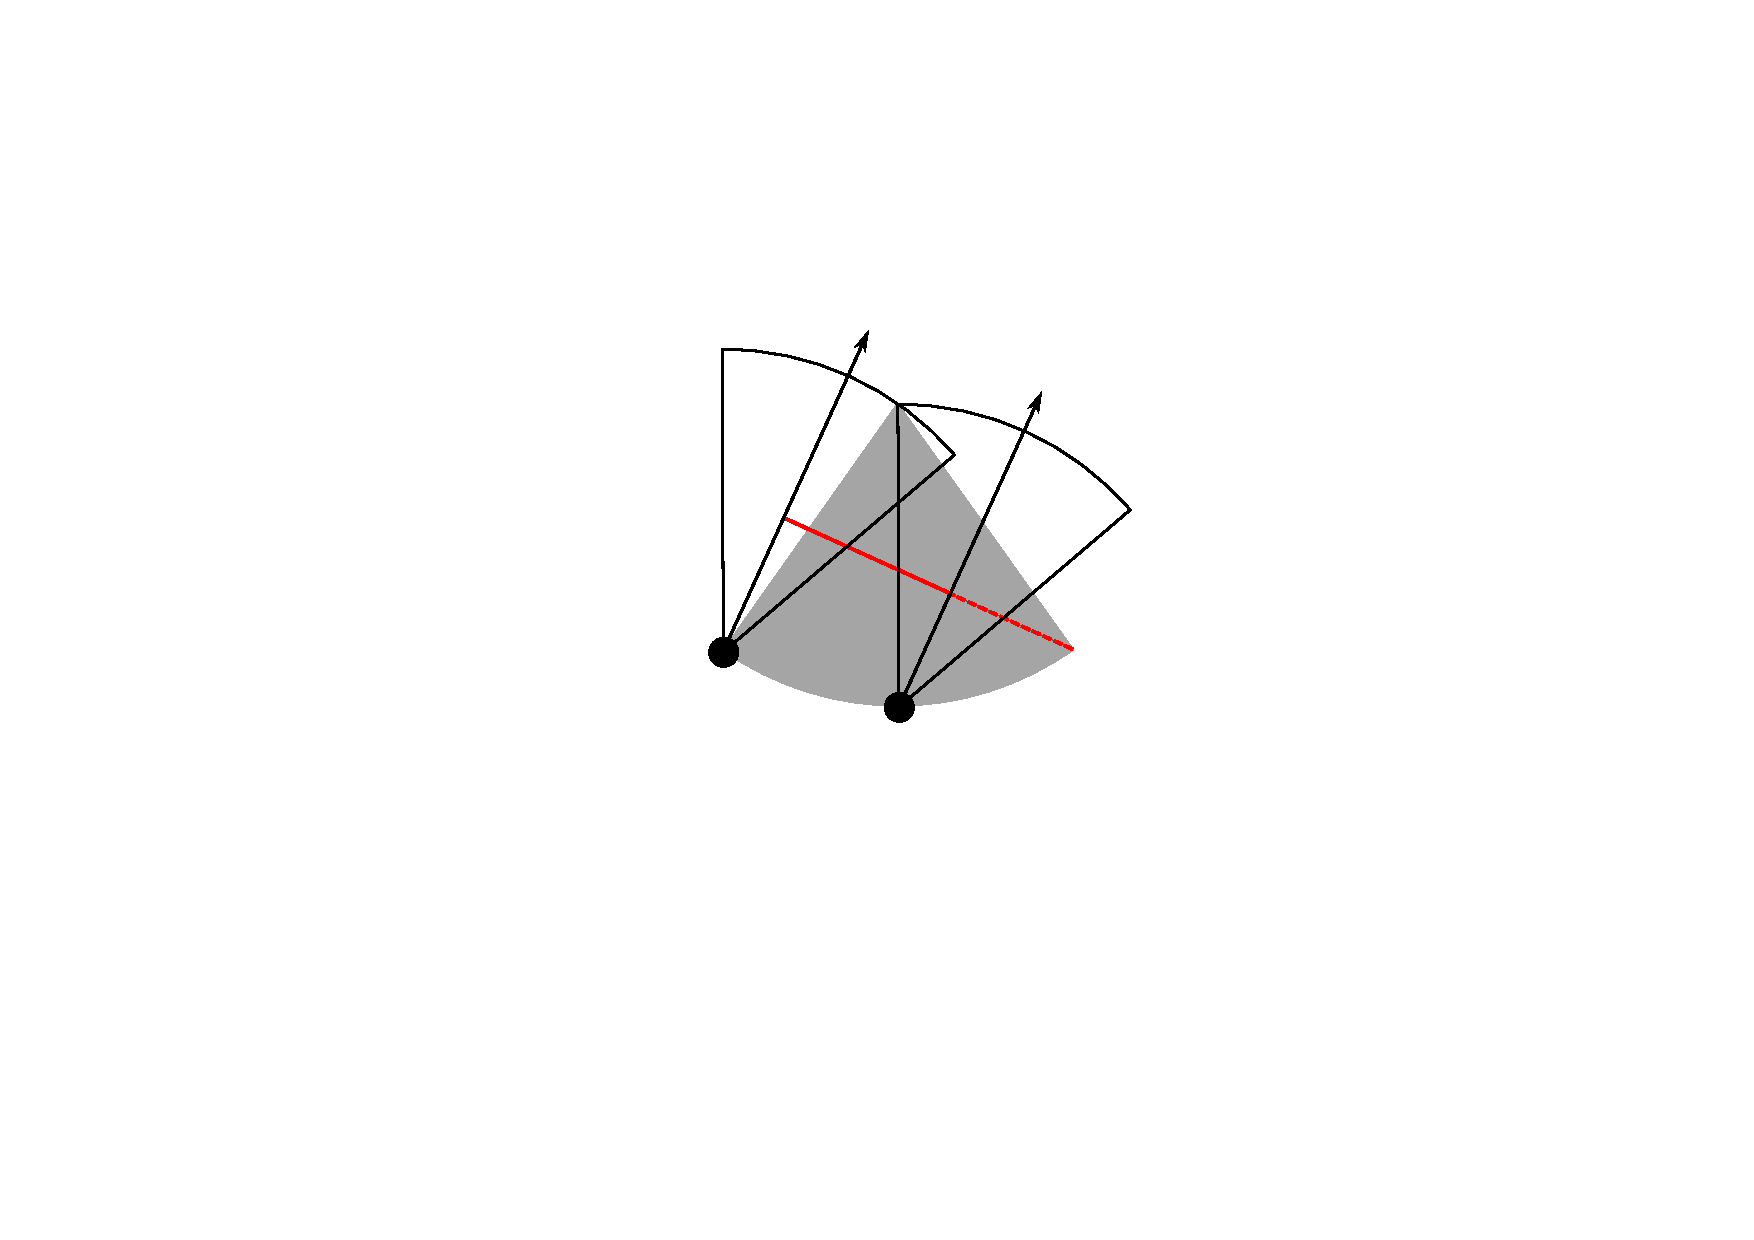
\includegraphics[width=.5\textwidth, trim=8cm 9cm 8cm 4cm]{imgs/4--9int3.pdf}
  }
}
\caption[Description of two profiles in SW models]{
Description of two profiles in SW models.
The sector shaped detection region is shown in grey.
Animals are filled black circles and the animal signal is an unfilled sector.
The animals direction of movement is indicated with an arrow.
The profile $p$ is shown with a red line.
Dashed red lines indicate areas where animals cannot be detected.
(a) At $x_4 = 0$, if $\alpha/2 < \pi/2 - \theta$ then $\alpha/2$ is too small for an animal to be detected at all during the $x_4$ profile (shown with dashed red).
This inequality simplifies to $\alpha < \pi - 2\theta$.
(b) The right of the profile is limited by the signal width, not the sensor.
On the left, the profile is limited by the sensor and not the signal.
Overall the profile width is $r\sin(\alpha/2) - r\cos(x_2 + \theta/2)$.
}
\label{fig:SW4--9}
\end{figure}

\subsubsection{Model SW4} \label{SW4}

SW4 is bounded by $\alpha \le \theta$, $\alpha \ge \pi - 2\theta$ and $\theta \le \pi/2$ (Figure~\ref{fig:equalRegions}).
Therefore it does contain a $x_4$ profile, starts with an $\alpha$ limited profile and does contain the $r\sin(\alpha/2) - r\cos(x_2 + \theta/2)$ profile in $x_2$.

\input{latexFiles/pSW4.tex}

\subsubsection{Model SW5} \label{SW5}

SW5 is the only model with a tetrahedral bounding region.
It is bounded by $\alpha \ge \theta$, $\alpha \ge \pi - 2\theta$, $\alpha \le 2\theta$ and $\theta \le \pi/2$ (Figure~\ref{fig:equalRegions}).
Therefore it does contain a $x_4$ profile, but starts with a $\theta$ limited profile.
It does contain the $r\sin(\alpha/2) - r\cos(x_2 + \theta/2)$ profile in $x_2$.

\input{latexFiles/pSW5.tex}

\subsubsection{Model SW6} \label{SW6}

SW6 is bounded by $\alpha \ge \pi - 2\theta$,  $\alpha \ge 2\theta$ and $\alpha \le \pi$ (Figure~\ref{fig:equalRegions}).
It starts with a $\theta$ limited profile and has a $x_4$ profile.
However, it does not contain the $r\sin(\alpha/2) - r\cos(x_2 + \theta/2)$ profile.

\input{latexFiles/pSW6.tex}


\subsubsection{Model SW7} \label{SW7}

SW7 is bounded by $\alpha \le \pi - 2\theta$, $\alpha \le \theta$ and $\alpha < 0$ (Figure~\ref{fig:equalRegions}).
Therefore it does not contain a $x_4$ profile.
It starts with an $\alpha$ limited profile and contains the $r\sin(\alpha/2) - r\cos(x_2 + \theta/2)$ profile in $x_2$.


\input{latexFiles/pSW7.tex}

\subsubsection{Model SW8} \label{SW8}

SW8 is bounded by $\alpha \le \pi - 2\theta$, $\alpha \ge \theta$ and $\alpha \le 2\theta$ (Figure~\ref{fig:equalRegions}).
It starts with a $\theta$ limited profile.
It does contain the $r\sin(\alpha/2) - r\cos(x_2 + \theta/2)$ profile in $x_2$ but does not have a $x_4$ profile.

\input{latexFiles/pSW8.tex}

\begin{comment}
\begin{figure}[t]
\centering
\includegraphics[width=1\textwidth]{imgs/equalModelResults.pdf}
\caption[REM model solutions]{The results of the models grouped so that all the regions with equal results are presented only once.}
\label{fig:equalModelResults}
\end{figure}
\end{comment}

\subsubsection{Model SW9} \label{SW9}

Finally, SW9, the last model, is bounded by y $\alpha \le \pi - 2\theta$, $\alpha \ge 2\theta$ and $\theta \ge 0$ (Figure~\ref{fig:equalRegions}).
Therefore it starts with a $\theta$ limited profile.
However it does not contain the extra $x_2$ profile nor a $x_4$ profile.

\input{latexFiles/pSW9.tex}








\vspace{1cm}




\clearpage
\section{Supplementary Information: Simulation model results of the gREM precision}
\setcounter{figure}{0}    




\begin{figure}[h!]
  \centering
	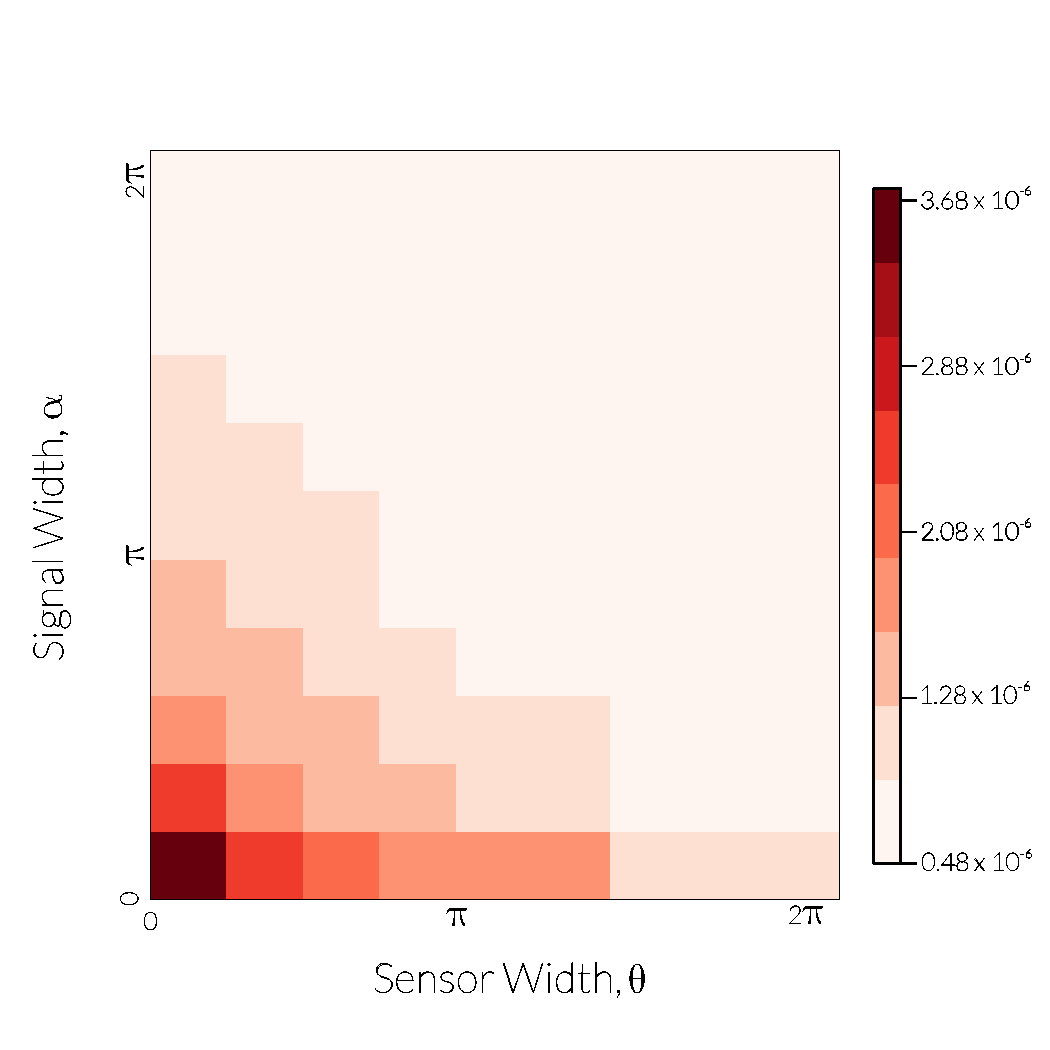
\includegraphics[width=\textwidth]{imgs/ResultStandardDeviation.pdf}
	\caption[gREM precision given a range of sensor and signal widths]{
Simulation model results of the gREM precision given a range of sensor and signal widths, shown by the standard deviation of the error between the estimated and true densities. 
Standard deviations are shown from deep red to pink, representing high to low values between $0.483\times10^{-6}$ to $3.74\times10^{-6}$. 
        } 
	\label{f:StandardDeviation}
\end{figure}


\clearpage
\section{Supplementary Information: Impact of parameter error}




\begin{figure}[h!]
  \centering
{
  \subfloat[label{f:signal}]{
    \includegraphics[width=0.4\textwidth]{imgs/AverageModelBias_callerror.pdf}
  } 
  \subfloat[label{f:sensor}]{
    \includegraphics[width=0.4\textwidth]{imgs/AverageModelBias_cameraerror.pdf}
  } 
    
	\subfloat[label{f:radius}]{
    \includegraphics[width=0.4\textwidth]{imgs/AverageModelBias_radiuserror.pdf}
  }%%
	\subfloat[label{f:speed}]{
    \includegraphics[width=0.4\textwidth]{imgs/AverageModelBias_speederror.pdf}
  }
}%%
\caption[Model sensitivity to error in parameter estimates]{
Model sensitivity (for all gREM submodels) to error in estimates of a) signal width $\alpha$,  b) sensor width $\theta$, c) detection distance $r$ and d) animal movement speed $v$. 
Estimates are -10\% (red), -1\% (orange), 0\% (grey), +1\% (green) and +10\% (blue) of the true parameter value. 
The black dashed line indicates zero error in density estimates. 
The error bars 95\% confidence intervals across all simulations.
}

\label{f:sensitivity}
\end{figure}












\chapter{Colophon}
\label{appendixlabel3}


This thesis was set using \LaTeX, \XeLaTeX\vspace{1mm} and Bib\LaTeX. \vspace{-0.12cm} 
The formatting is defined by the \href{https://github.com/robjstan/latex-phdthesis}{\emph{phdthesis}} class by Robert Stanley.
The TeX Gyre Pagella typeface is used in the main text while {\usefont{T1}{fla}{l}{n} Lato Light} and {\usefont{T1}{fla}{eb}{n} \color[rgb]{0.75,0.75,0.75} Lato Black} are used in the figures.
Chapters \ref{ch:empirical}, \ref{ch:sims1} and \ref{ch:sims2} are entirely reproducible \href{http://yihui.name/knitr/}{\emph{knitr}} documents \cite{knitr}.
Code for the simulations in Chapter \ref{ch:grem} is not combined into a \emph{knitr} document but code for creating figures is.
All code will be made available on Github at \href{https://github.com/timcdlucas/PhDThesis}. %TODO add dois for thesis and MetapopEpi
Plots were created with a combination of \href{www.inkscape.org}{\emph{Inkscape}}, \emph{ggplot2} \cite{ggplot2}, \emph{palettetown} \cite{palettetown}, \emph{ggtree} \cite{ggtree}, \emph{cowplot} \cite{cowplot} and base \emph{R} \cite{R}.
References were handled with \emph{JabRef} \cite{JabRef_software}. 
 % description of document, e.g. type faces, TeX used, TeXmaker, packages and things used for figures. Like a computational details section.
% e.g. http://tex.stackexchange.com/questions/63468/what-is-best-way-to-mention-that-a-document-has-been-typeset-with-tex#63503

 
% You could separate these out into different files if you have
%  particularly large appendices.

% This line manually adds the Bibliography to the table of contents.
% The fact that \include is the last thing before this ensures that it
% is on a clear page, and adding it like this means that it doesn't
% get a chapter or appendix number.
\addcontentsline{toc}{chapter}{Bibliography}

% Actually generates your bibliography.
\bibliography{../../epilit}

% All done. \o/
\end{document}
